% v3.0 released 22 May 2015

%%%%%%%%%%%%%%%%%%%%%%%%%%%%%%%%%%%%%%%%%%%%%%%%%%
\documentclass[fleqn,usenatbib,useAMS]{mnras}

\usepackage{graphicx}	% Including figure files
\usepackage{amsmath}	% Advanced maths commands
\usepackage{amssymb}	% Extra maths symbols
\usepackage{multicol}        % Multi-column entries in tables
\usepackage{bm}		% Bold maths symbols, including upright Greek
\usepackage{pdflscape}	% Landscape pages
\usepackage{enumitem}	% Including figure files
\usepackage{multirow}   % Allow multi-row cells in tables
\usepackage{xspace}
\usepackage{CJK}
\usepackage{longtable}
\usepackage{xcolor}
\usepackage{etoolbox}
\makeatletter
\makeatother
%%%%%%%%%%%%%%%%%%%%%%%%%%%%%%%%%%%%%%%%%%%%%%%%%%
\newcommand{\Teff}{$T_\mathrm{eff}$\xspace}
\newcommand{\logg}{$\log g$\xspace}
\newcommand{\feh}{$\mathrm{[Fe/H]}$\xspace}
\newcommand{\fehatmo}{$\mathrm{[Fe/H]}_\text{atmo}$\xspace}
\newcommand{\alphafe}{$\mathrm{[\upalpha/Fe]}$\xspace}
\newcommand{\vmic}{$v_\mathrm{mic}$\xspace}
\newcommand{\lbol}{$L_\mathrm{bol}$\xspace}
\newcommand{\vmac}{$v_\mathrm{mac}$\xspace}
\newcommand{\vsini}{$v \sin i$\xspace}
\newcommand{\vbroad}{$v_\mathrm{broad}$\xspace}
\newcommand{\vrad}{$v_\mathrm{rad}$\xspace}
\newcommand{\numax}{$\nu_\mathrm{max}$\xspace}
\newcommand{\Gaia}{\textit{Gaia}\xspace}
\newcommand{\Hipparcos}{{\sc{Hipparcos}}\xspace}
\newcommand{\tess}{\textit{TESS}\xspace}
\newcommand{\Ktwo}{\textit{K2}\xspace}

\definecolor{C0}{rgb}{0.12156862745098039, 0.4666666666666667, 0.7058823529411765}
\definecolor{C1}{rgb}{1.0 0.4980392156862745 0.054901960784313725}
\definecolor{C2}{rgb}{0.17254901960784313 0.6274509803921569 0.17254901960784313}
\definecolor{C3}{rgb}{0.8392156862745098 0.15294117647058825 0.1568627450980392}
\definecolor{C4}{rgb}{0.5803921568627451 0.403921568627451 0.7411764705882353}

\newcommand\SB[1]{\textcolor{blue}{SB: #1}}
\newcommand\TN[1]{\textcolor{red}{TN #1}}
\newcommand\AMA[1]{\textcolor{violet}{AMA: #1}}
\newcommand\YST[1]{\textcolor{orange}{YST: #1}}
\newcommand\DN[1]{\textcolor{purple}{DN: #1}}
\newcommand\LS[1]{\textcolor{green}{LS: #1}}
\newcommand\SLM[1]{\textcolor{cyan}{SLM: #1}}
\newcommand\KL[1]{\textcolor{magenta}{KL: #1}}

%%%%%%%%%%%%%%%%%%%%%%%%%%%%%%%%%%%%%%%%%%%%%%%%%%
\usepackage[T1]{fontenc}
\usepackage{ae,aecompl}
\usepackage{newtxtext,newtxmath}

%@arxiver{lb_overview_colored.png, galah_dr3_comparison_dr2.png, dr3_abundance_overview_31_elements.png}

\begin{document}
\begin{CJK*}{UTF8}{gbsn}
\label{firstpage}
\pagerange{\pageref{firstpage}--\pageref{lastpage}}

%%%%%%%%%%%%%%%%%%% TITLE PAGE %%%%%%%%%%%%%%%%%%%

\title{The GALAH+ Survey: Third Data Release}

% The list of authors, and the short list which is used in the headers.
% If you need two or more lines of authors, add an extra line using \newauthor
\author[Buder et al.]{Sven Buder$^{1,2,3}$\thanks{Contact e-mail: \href{mailto:sven.buder@anu.edu.au}{sven.buder@anu.edu.au}},
Sanjib~Sharma$^{4,3}$, 
Janez~Kos$^{5}$,
Anish~M.~Amarsi$^{6,1}$, \newauthor
Thomas~Nordlander$^{2,3}$, 
Karin~Lind$^{7,1}$,
Sarah~L.~Martell$^{8,3}$, 
Martin~Asplund$^{2,3}$, \newauthor 
Joss~Bland-Hawthorn$^{4,3}$,
Andrew~R.~Casey$^{9,10}$, 
Gayandhi~M.~De~Silva$^{11,12}$, \newauthor
Valentina~{D'Orazi}$^{13}$,
Ken~C.~Freeman$^{2,3}$,  
Michael~R.~Hayden$^{4,3}$,
Geraint~F.~Lewis$^{4}$,   \newauthor
Jane~Lin$^{2,3}$, 
Katharine.~J.~Schlesinger$^{2}$,
Jeffrey~D.~Simpson$^{8,3}$, 
Daniel~B.~Zucker$^{12,14}$, \newauthor
Toma\v{z}~Zwitter$^{5}$,  
David~M.~Nataf$^{15}$,
Yuan-Sen~Ting (丁源森)$^{16,17,18,2}$,  \newauthor
and~the~GALAH~collaboration, 
(co-author order TBD according to SOFA)
\\
\\
(Affiliations listed after the references)}

% These dates will be filled out by the publisher
\date{Accepted 2020 Month Day. Received 2020 September 1}

% Enter the current year, for the copyright statements etc.
\pubyear{2020}

% Don't change these lines
\maketitle
\end{CJK*}

% Abstract of the paper
\begin{abstract}
The recent dramatic increase in spectroscopic, astrometric and photometric data has highlighted the scientific opportunities afforded by obtaining an ensemble of chemical element abundances for stars with precision distances and orbit measurements. With this third data release of the Galactic Archaeology with HERMES (GALAH) survey, we publish 694 459 spectra for 600 255 mostly nearby stars, that have been observed with the HERMES spectrograph at the Anglo-Australian Telescope.

This release, referred to as GALAH+ DR3, includes all observations from GALAH Phase 1 (both main and faint survey), the K2-HERMES and TESS-HERMES surveys as well as additional GALAH-related projects including bulge and observations of more than 80 stellar clusters.

With this data release we improve our spectrum analysis with external astro- and photometric information from \Gaia DR2 and 2MASS to estimate more accurate stellar surface gravities than before, thus breaking spectroscopic degeneracies. We estimate stellar parameters of \Teff, \logg, \feh, \vmic, \vbroad, and \vrad as well as 30 element abundances, [X/Fe], via the spectrum synthesis code Spectroscopy Made Easy (SME) with 1D {\sc marcs} stellar atmosphere models. We use non-LTE computations for eleven elements to estimate element abundances line-by-line for as many elements as feasible. We report and catalogue element abundances of Li, C, O, Na, Mg, Al, Si, K, Ca, Sc, Ti, V, Cr, Mn, Fe, Co, Ni, Cu, Zn, Rb, Sr, Y, Zr, Mo, Ru, Ba, La, Ce, Nd, Sm, and Eu which are from five nucleosynthetic pathways. We describe our validations for accuracy and precision, flagging of peculiar stars or measurements and stress that all users should take these flags into account.

Our catalogue comprises 374 229 (66\%) dwarfs and 183 467 (33\%) giants, including roughly 59\% low-alpha disk stars, 19\% high-alpha disk stars, and 5\% kinematic halo stars, as well as 90 321 and 29 721 stars overlapping with K2 and TESS, respectively.  Several Value- Added-Catalogs for stellar ages, stellar dynamics, detailed abundance measurements, and binary systems accompany this data release. Together they provide a high-dimensional data set to study the chemodynamic evolution of the local (80.4\% of stars within 2 kpc) Milky Way, as we showcase with a few chemodynamic analyses. 
\end{abstract}

% Select between one and six entries from the list of approved keywords.
% Don't make up new ones.
\begin{keywords}
Surveys -- 
the Galaxy --
methods: observational --
methods: data analysis --
stars: fundamental parameters -- 
stars: abundances
\end{keywords}

%%%%%%%%%%%%%%%%%%%%%%%%%%%%%%%%%%%%%%%%%%%%%%%%%%

%%%%%%%%%%%%%%%%% BODY OF PAPER %%%%%%%%%%%%%%%%%%

\newpage
%________________________________________________________________
\section{Introduction} \label{sec:introduction}

\KL{Keep citations in introduction balanced to represent the field as a whole. Are all groups represented?}
% This figure was created with the notebook GALAH_DR3/input/galah_dr3_input.ipynb
\begin{figure*}
\centering
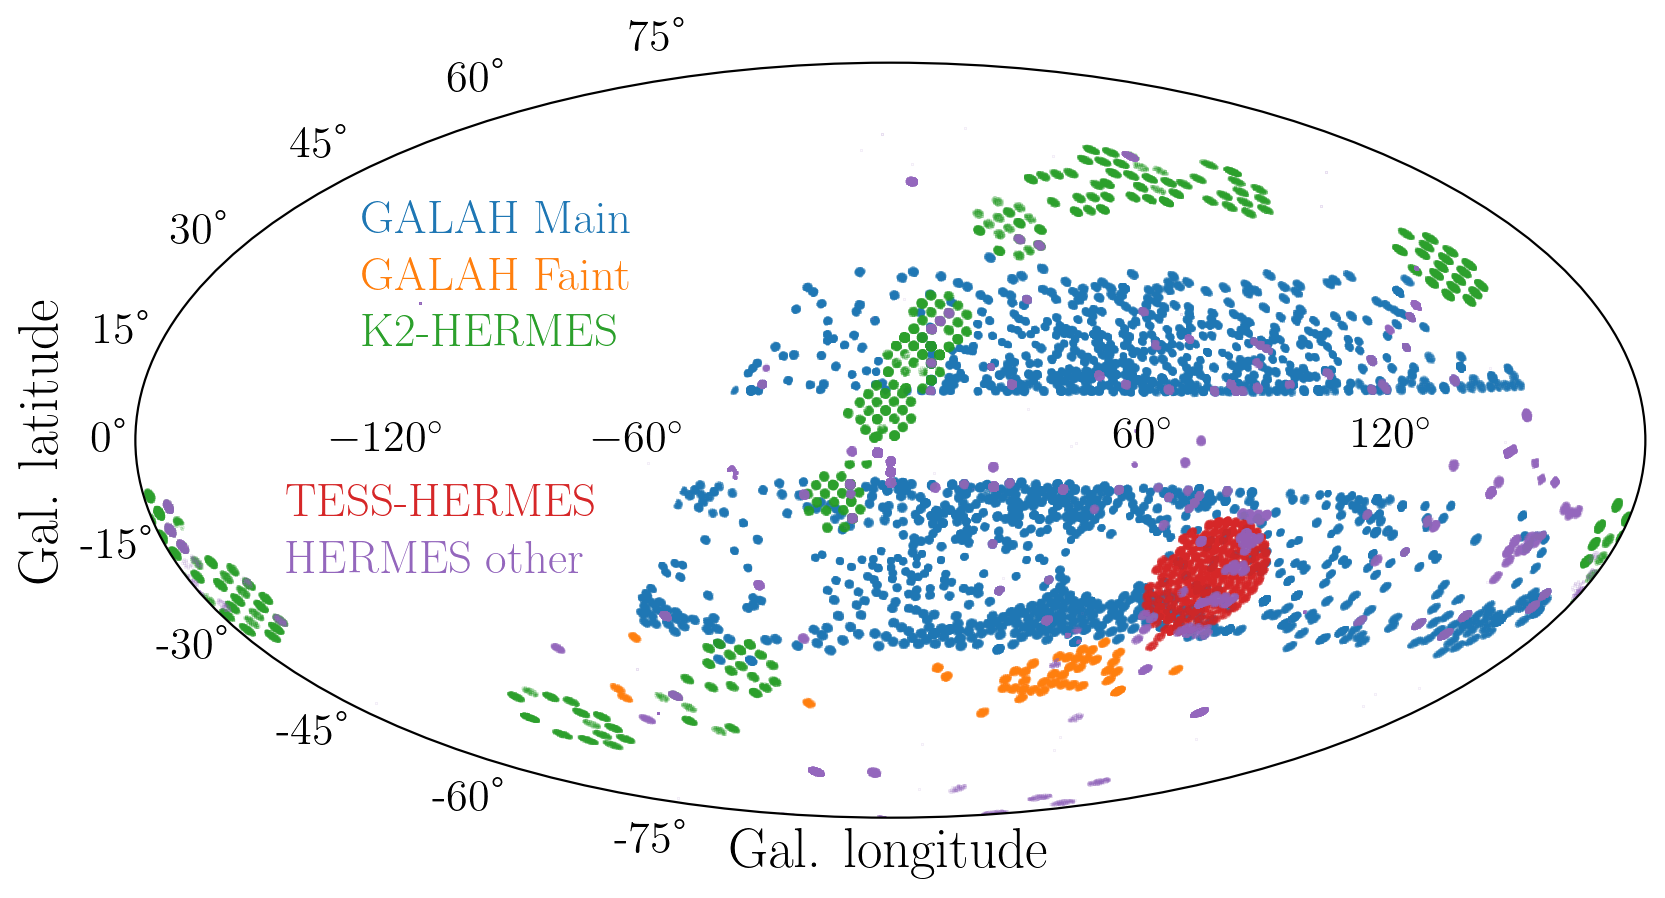
\includegraphics[width=\textwidth]{figures/lb_overview_colored.png}
\caption{\textbf{Overview of the distribution of stars observed as part of this data release in Galactic coordinates with the centre of the Galaxy at the origin.} Shown are the GALAH main (blue) and faint (orange) targets, which avoid the Galactic plane. The targets of the \Ktwo-HERMES follow-up (green) fall within with the \Ktwo\ campaigns along the ecliptic and show the characteristic tile-pattern of the \textit{Kepler} telescope. The \tess-HERMES observations (red) are focused on the \tess\ Southern Continuous Viewing Zone. Other HERMES targets (purple) are distributed across the sky and were observed during several independent programs.}
\label{fig:lb_overview_colored}
\end{figure*}

Until recently, the data available to answer the question of how the Milky Way formed and evolved was limited to a few hundred or thousand stars with high-quality element abundances in our Solar neighbourhood \citep[see e.g.][]{Edvardsson1993, Nissen2010, Bensby2014}. With the advances in multi-object observations both in space and on the ground, the field of Galactic Archaeology is in a transformation from single-star population studies towards large-scale structural analyses. Due to the intrinsic difficulty in determining the distances of stars, studies of the chemodynamical evolution of our Milky Way were previously restricted to nearby stars, which were mapped by the \Hipparcos satellite \citep{ESA1997, Perryman1997, vanLeeuwen2007}. In the era of the \Gaia satellite \citep{Gaia-Collaboration2016, Gaia2016, Brown2018}, we can now use astrometric and photometric observables and their physical relations with spectroscopic quantities to improve the analysis of spectra and thus the estimation of element abundances.

The connections between the chemical compositions and dynamics of stars across the vast populations in our Galaxy are a topic of significant ongoing research. Although we speak of the Milky Way in terms of the thin and thick disc \citep{Yoshii1982, Gilmore1983}, the bulge \SLM{needs a reference}, and the stellar halo \citep[see e.g.][]{BlandHawthorn_Gerhard2016} as its main components, we understand that the Galaxy is more than a superposition of independent populations. With the data now at hand, we can analyse the Galaxy from a chemodynamical perspective and use stars of different ages as time capsules to trace back the formation history of our Galaxy \citep[see e.g.][]{Rix2013, BlandHawthorn2019}. As one example, the most recent data release from \Gaia\ has enabled significant leaps in our understanding of the enigmatic halo \citep[for an overview see][]{Helmi2020}. 6-d phase space information from \Gaia\ has revealed a large population of stars in the Solar neighbourhood that stand out against the smooth halo background as a coherent dynamical structure, pointing to a significant accretion event that is currently referred to as either ``\Gaia-Enceladus'' \citep{Helmi2018} or ``the \Gaia\ Sausage'' \citep{Belokurov2018}. Additionally, while we would expect the chemical composition of stars to be correlated with their ages and formation sites \citep[see e.g.][]{Minchev2017}, observations can now clearly demonstrate these connections \citep[see e.g.][]{Feuillet2018, Buder2019}, and can also demonstrate that stars within our Solar neighborhood have migrated significantly  \citep[see e.g.][]{Frankel2018, Hayden2020}. We have, however, not uncovered the formation history of our Galaxy in full detail, and many puzzle pieces are presently missing or contentious, including the discrete merger history of our Milky Way, the (non-)existence of an \textit{in situ} halo, or the reason for the sharp transition from formation of stars with high $\upalpha$-element abundances in what has historically been called the ``thick disc'' to younger stars with Solar-like $\upalpha$-element abundances in the ``thin disc''.

Previous and ongoing spectroscopic survey projects by collaborations like RAVE \citep{Steinmetz2020a, Steinmetz2020b}, Gaia-ESO \citep{Gilmore2012}, SDSS-IV APOGEE \citep{SDSSDR16}, and LAMOST \citep{Cui2012, Xiang2019} have certainly helped to shed light on several of these outstanding questions. Answering them completely requires more and/or better data to map out the correlations between stellar ages, abundances, and dynamics. Upcoming surveys like SDSS-V \citep{Kollmeier2017}, WEAVE \citep{WEAVE2018}, and 4MOST \citep{4MOST2019} will certainly broaden our capabilities, expanding horizon not only quantitatively. The data currently at hand, including photometry, spectroscopy, astrometry, and asteroseismology, are a powerful set of high-dimensional information, and we must develop methods to extract the most accurate and precise information from them \citep[for reviews on this see e. g.][]{Jofre2018b, Nissen2018}.

Chemical tagging, by which we mean identifying stars that formed together using their chemical composition and understanding the astrophysics driving the dimensionality of chemical space, will be key for observationally unlocking the building blocks of our Galaxy and therefore remains a major science driver for the GALAH collaboration \citep{DeSilva2015}. With the large variety of nucleosynthetic channels that can enrich the birth material of stars \citep[see e.g.][]{Kobayashi2020}, the hypothesis is that we should be able to disentangle stars with different enrichment patterns, if we observe enough elements with different enrichment origins. The success of some chemical tagging experiments \citep[see e.g.][]{Kos2018, PriceJones2020} is challenged by the broad similarities in abundance in populations like the low-$\upalpha$ disk \citep[see e.g.][]{Ness2018} and small but real inhomogeneities even within star clusters \citep{Liu2016,Liu2016b}. To put detailed chemical tagging into action, we will need a massive data set \citep[see e.g.][]{Ting2016} and an outstanding precision in our measurements.

For the second data release of the GALAH survey \citep{Buder2018} we made use of data-driven approaches to improve both speed and precision of the spectroscopic analysis. This was performed almost entirely without non-spectroscopic information for individual stars, using a ``training set'' of stars with careful by-hand analysis.
Although the data-driven approaches were successful for the majority of GALAH DR2 stars, we know that these approaches can suffer from signal aliasing, they can learn unphysical correlations between the input data and the output stellar labels, and the results are not necessarily valid outside the parameter space of the training set. As part of the present study, we aim to asses how accurately the stellar parameters and abundances were estimated with the data-driven approaches. 

The publication of \Gaia DR2 \citep{Brown2018, Lindegren2018} provided 5-dimensional phase space information (coordinates, proper motions, and parallax) for 1.3 billion stars, and having this information available for essentially all stars in GALAH has brought major improvements to our stellar analysis. By combining our knowledge of the (absolute) photometry and spectroscopy of stars, we can break several of the degeneracies in stand-alone spectroscopic analysis, because absorption lines in spectra change smoothly, but not always significantly as a function of stellar atmospheric parameters. The data analysis process for this third data release from the GALAH collaboration makes use of these fundamental correlations, and this quantifiably improves the accuracy and precision of our measurements.

As large Galactic Archaeology-focused survey projects continue to collect data, the overlap between them increases. This enables us to compare results when analysing stars in the overlap, which have the same stellar labels, and it also allows us to propagate labels from one survey onto another \citep[see e.g.][]{Casey2017, Ho2017, Xiang2019, Wheeler2020}. This label propagation makes it possible to combine these complementary surveys for global mapping of stellar properties and abundances, and we show an example of this in Section \ref{sec:galah_in_context}, placing GALAH DR3 data in context with the APOGEE and LAMOST surveys.

This paper is structured as follows: We describe our target selection (coordinated by working group 1), observations (coordinated by WG2), and reductions (WG3) in Sec.~\ref{sec:selection_observation_reduction}. While the target selection and observation of the several projects like \Ktwo-HERMES and \tess-HERMES were slightly different from the main GALAH survey, we have reduced and analysed all data (combined under the term GALAH+) in the same way. The analysis of the reduction products is described in Sec.~\ref{sec:analysis}, focusing on the description of the general workflow of the analysis group (WG4) and highlighting changes with respect to the previous release (GALAH DR2). Secs.~\ref{sec:validation_sp} and \ref{sec:validation_ab} address the validation efforts for stellar parameters and element abundances, respectively. These address the accuracy and precision of these labels as well as our algorithms to identify and flag peculiar measurements or peculiar stars. Based on experience with the data set, we stress the importance of the flags, but also how complex the flagging estimates are, with several examples of peculiar abundance patterns. We also highlight possible caveats (or possibly peculiar physical correlations) of our analysis in Sec.~\ref{sec:caveats}. We present the contents of the main catalog of this data release in Sec.~\ref{sec:catalogs}. In this section we also present the Value Added Catalogs (VACs) that accompany this release, including stellar dynamics and age estimates and a description of how these were derived. We then use these together with the element abundances of the main catalog in Sec.~\ref{sec:galah_in_context} to highlight the scientific potential of the release data in context, focusing on Galactic archaeology on a global scale and the chemodynamical evolution of our Galaxy. 

Along with the main and value-added catalogs of this release, we publish the observed spectra on the DataCentral\footnote{\url{https://docs.datacentral.org.au/galah/}} and provide the scripts used for the analysis as well as post-processing online in an open-source repository\footnote{\url{http://github.com/svenbuder/GALAH\_DR3}}

% This figure was created with the notebook GALAH_DR3/input/galah_dr3_input.ipynb
\begin{figure*}
\centering
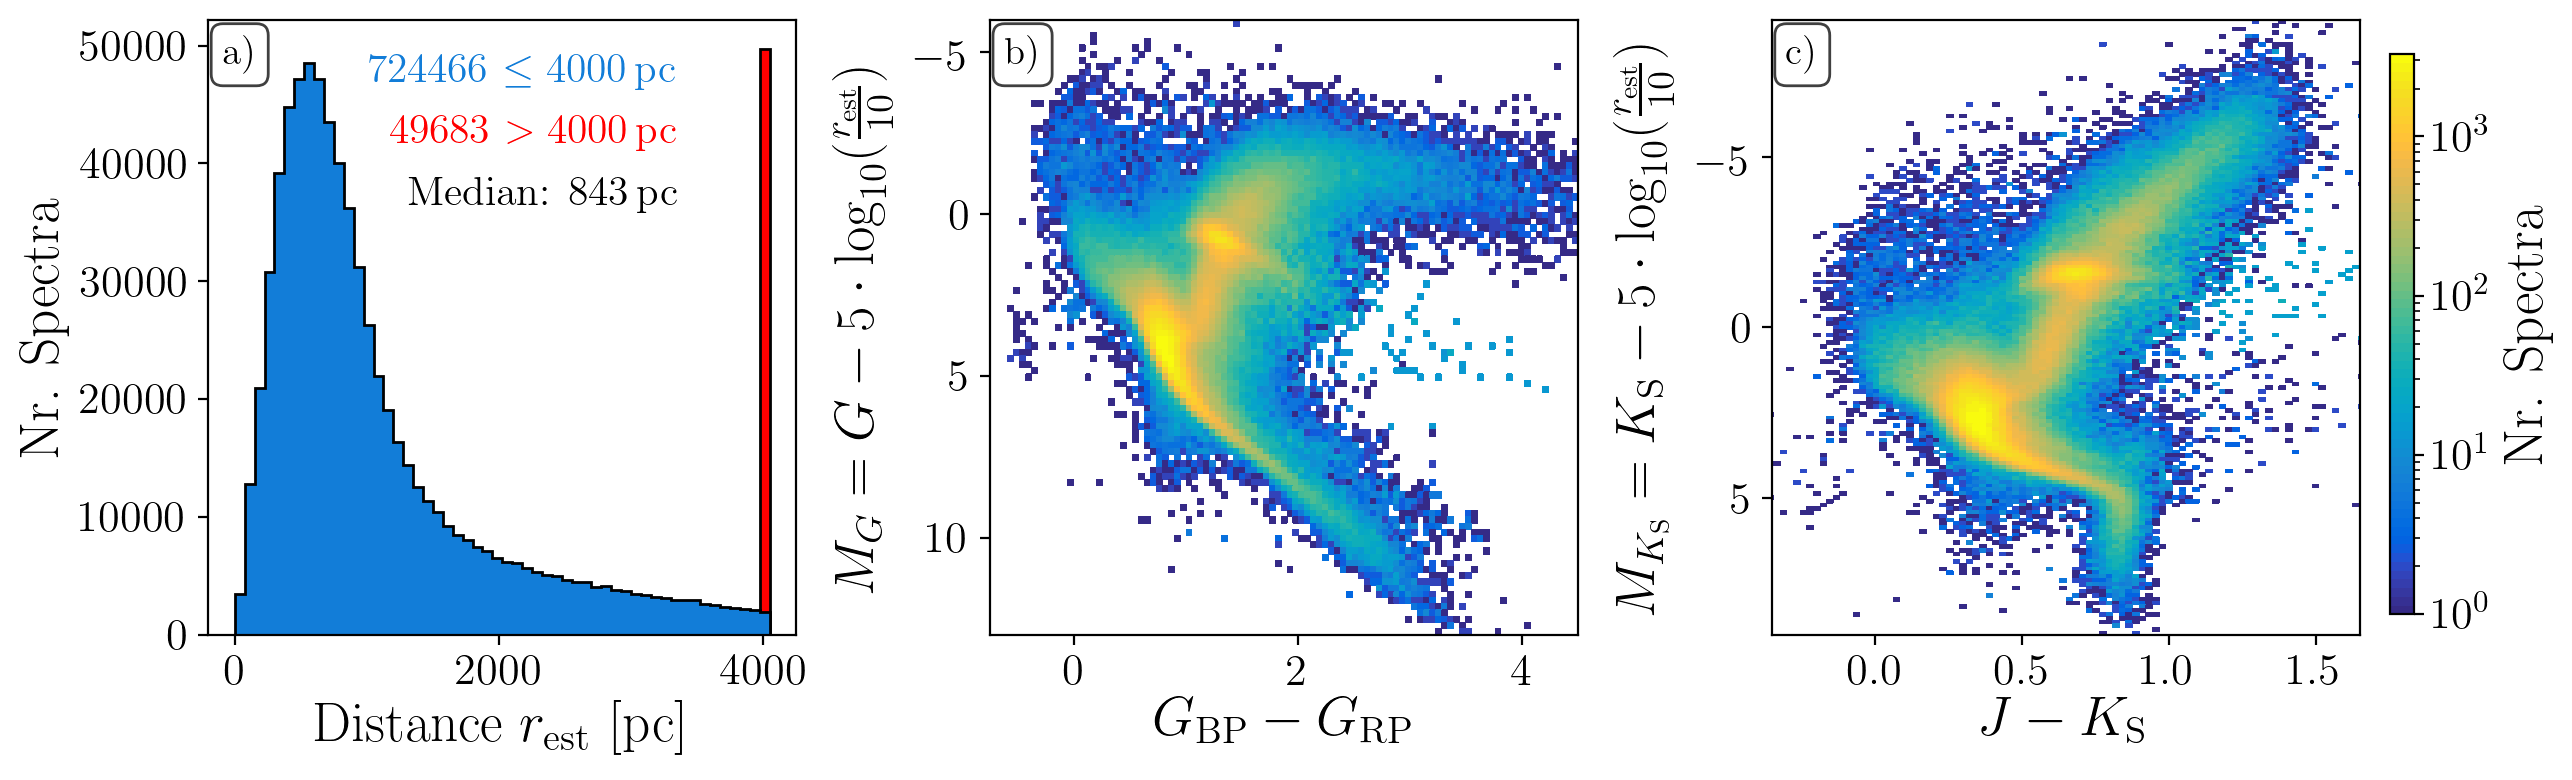
\includegraphics[width=\textwidth]{figures/plot_parallax_quality_and_cmds.png}
\caption{
\textbf{Overview of distances and photometric information for the spectra (including repeats for some stars) observed as part of GALAH DR3 up to 25th February 2019.}
\textbf{Panel a)} shows the distances of stars in GALAH DR3. Due to the magnitude limited selection of stars, the majority of stars are not only dwarfs but also nearby; that is, within $1\,\mathrm{kpc}$. Only $4.7\%$ of stars are beyond $4\,\mathrm{kpc}$ (truncated in red in the histogram). 
\textbf{Panel b)} shows a reddened color-absolute magnitude diagram in the optical \Gaia passbands.
\textbf{Panel c)} shows an analogous diagram made with the infrared 2MASS passbands.
\KL{Can the x-axes of the left-hand panel of Figs. 2 and 3 be made logarithmic instead of truncated?}
}
\label{fig:plot_parallax_quality_and_cmds}
\end{figure*}

%________________________________________________________________
\section{Target selection, observation, reduction} \label{sec:selection_observation_reduction}

While our previous data release \citep{Buder2018} contained only stars from the main GALAH survey, the current catalog is the combination of multiple projects with different science goals, all conducted with the HERMES spectrograph \citep{Sheinis2015} and the 2dF fibre positioning system \citep{Lewis2002} at the 3.9-metre Anglo-Australian Telescope. There are four main projects, plus a number of smaller observing programs, included in GALAH DR3. Figure \ref{fig:lb_overview_colored} shows their on-sky distribution. The majority of the stars are nearby with a median distance of $843\,\mathrm{pc}$ (see panel a of Fig.~\ref{fig:plot_parallax_quality_and_cmds}) and cover a large variety of stellar types and evolutionary stages, as can be seen in the colour-magnitude diagrams both with \Gaia (panel b) and 2MASS (panel c) filters. Below we describe the target selection for each of the four main projects.

\subsection{Target selection}

The initial GALAH input catalog was made by combining the 2MASS \citep{Skrutskie2006} catalog of infrared photometry with the UCAC4 \citep{Zacharias2013} proper motion catalogue. We only included stars with reliable 2MASS data, as captured in their data quality flags (Q=``A'', B=``1'', C=``0'', X=``0'', A=``0'', prox$\ge 6\arcsec$). We also rejected any star that had a nearby bright neighbour, with a rejection radius dependent on the bright star's $V$ magnitude, such that the potential target is rejected if the bright star is closer than $(130-[10\times V])$ arcseconds. The APASS photometric catalogue \citep{Henden2012} was not complete in the Southern sky at the start of GALAH observations in 2013, so we use a synthetic $V_\mathrm{JK}$ magnitude calculated from 2MASS photometry: $V_\mathrm{JK} = K+2(J-K+0.14)+0.382e^{((J-K-0.2)/0.5)}$. \citet{Sharma2018} demonstrate using PARSEC isochrones \citep{Marigo2017} that this is a reasonable approximation for the $V$ magnitude for the types of stars observed in GALAH.

The four main projects included in the GALAH DR3 catalogue are GALAH-main, GALAH-faint, \Ktwo-HERMES, and \tess-HERMES, and each has its own selection function. We have attributed each possible pointing of the major sub surveys to a specific $\texttt{field\_id}$, as listed in Table~\ref{tab:field_ids}. The main GALAH survey takes as potential targets all stars with $12.0<V<14.0$, $\delta < +10^{\circ}$ and $|b|>10^{\circ}$ in regions of the sky that have at least 400 targets in $\pi$ square degrees (the 2dF field of view). We then segment this data set into 6546 ``fields'' with a fixed centre and radius between 0.7 and 1 degree. Fields containing more than 400 stars are observed multiple times with separate target lists. The main survey also includes an extension for bright targets ($9.0<V<12.0$) to be observed in twilight or poor observing conditions. For bright stars we use the same field centres as in regular survey observing, and require at least 200 stars per field.

The GALAH-faint program was aimed at extending survey observations to higher Galactic latitude. Given the lower density of stars when looking higher in the Galactic plane, the target selection was shifted to $14<V<16$ as a way to maintain at least 400 stars per field. These fields were only observed under dark conditions.

The \Ktwo-HERMES survey leverages the excellent match between the two degree diameter of the 2dF fibre positioner and the five square degrees covered by each detector in the \textit{Kepler} spacecraft to create an efficiently observed spectroscopic complement for red giant branch stars in the \Ktwo\ campaign fields. The \Ktwo-HERMES program has both ``bright'' ($10<V<13$) and ``faint'' ($13<V<15$, $J-K_S>0.5$) target cohorts, to complement the asteroseismic targets that are the focus of the \Ktwo\ Galactic Archaeology Program \citep{Stello2017}. Analysis of asteroseismic and spectroscopic data together is key for GALAH DR3, and enables in-depth exploration of the structure and history of the Milky Way \citep[e.g.,][]{Sharma2016,Sharma2019}. The spectroscopic data also provide essential insights for planet hosting stars identified in \Ktwo\ data \citep{Wittenmyer2018,Wittenmyer2020}.

The \tess-HERMES survey collected spectra for stars in the range $10.0<V<13.1$ in the \tess\ Southern Continuous Viewing Zone, within 12 degrees of the Southern ecliptic pole. \tess-HERMES aimed to provide accurate stellar parameters for candidate \tess\ input catalog stars \citep{Stassun2019}, to better focus \tess\ target selection on the most promising asteroseismic targets. The results of the \tess-HERMES project are publicly available, and project and outputs are described in \citet{Sharma2018}.

Stars in the ``HERMES other'' program are from targeted observations in open clusters, the GALAH Pilot Survey \citep{Martell2017}, or targets from other HERMES observing that were not part of any of these surveys.

% Made with GALAH_DR3/validation/comparisons/Galactic_Archaeology_In_Context.ipynb
\begin{figure*}
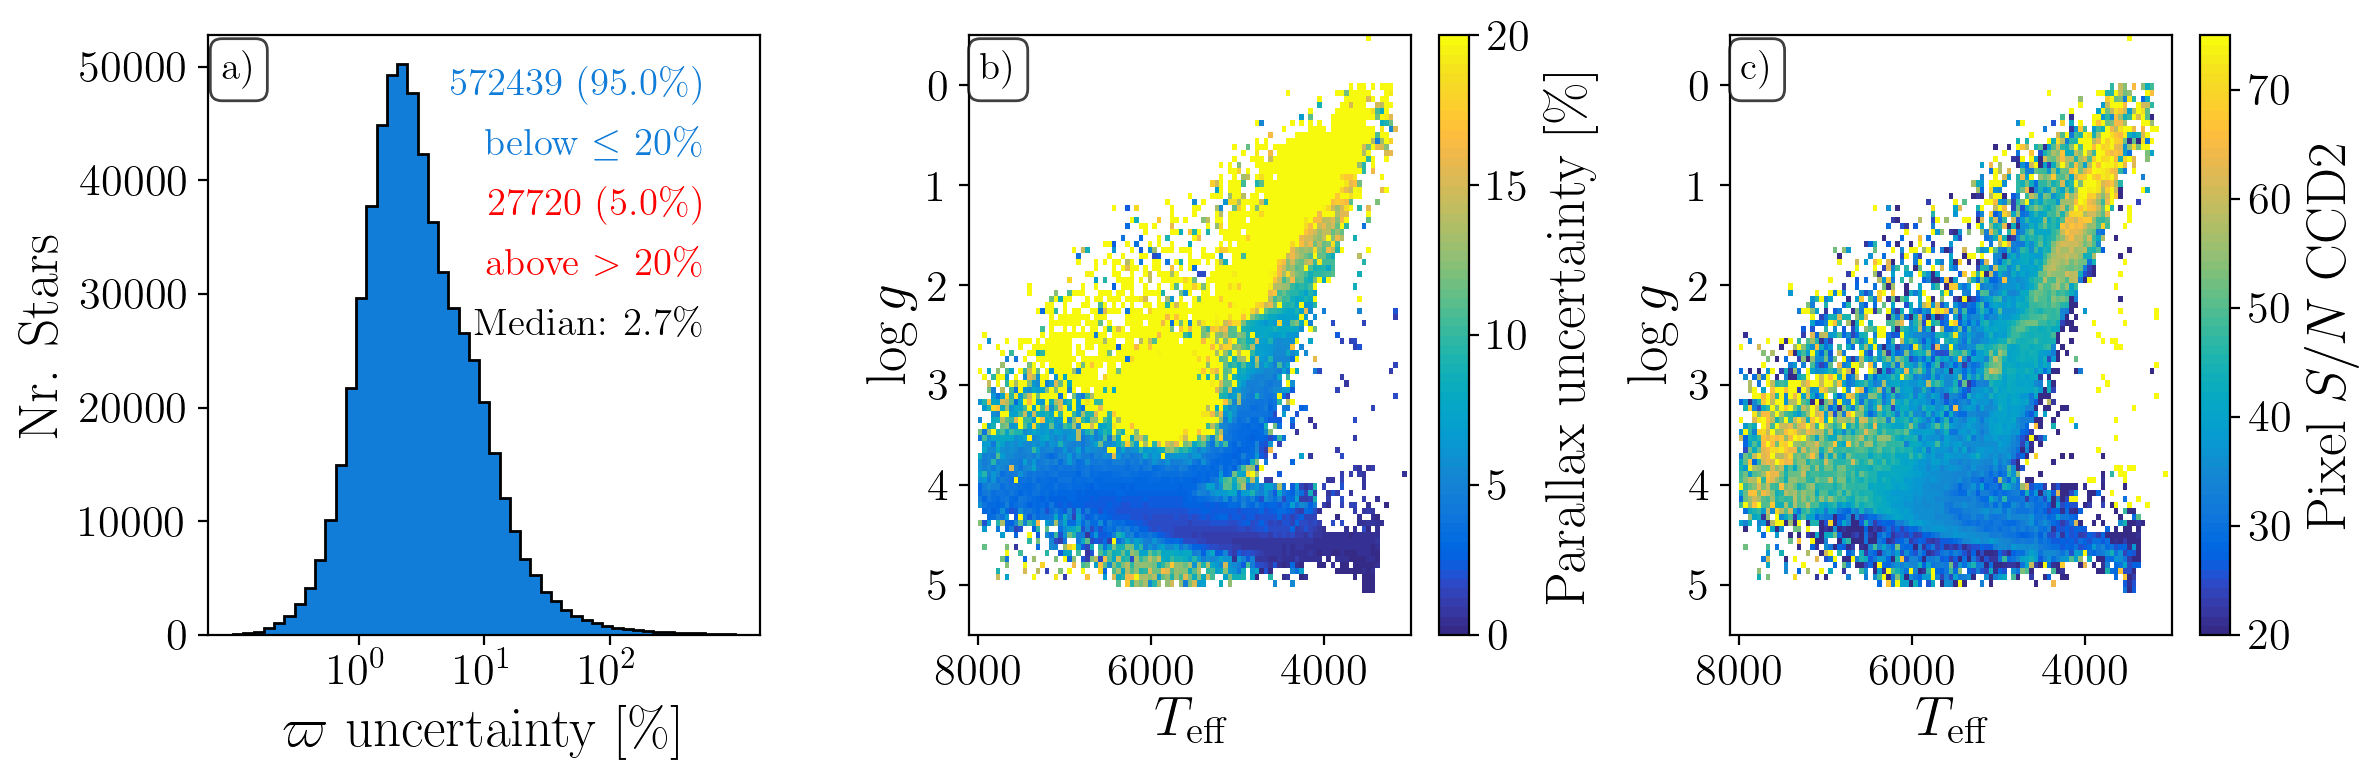
\includegraphics[width=\textwidth]{figures/plot_distance_tefflogg_distance_snr.png}
  \caption{
\textbf{Overview and distribution of parallax uncertainty and $S/N$ for different types of stars (not spectra as in Fig.~\ref{fig:plot_parallax_quality_and_cmds}).}
\textbf{Panel a)} Parallax ($\varpi$) uncertainty provided by \Gaia DR2. 702~945 (91\%) stars sit below 15\% in fractional uncertainty (blue), and 71~204 (9\%) stars fall above 15\% (red, truncated). 
\textbf{Panel b)} Distribution of fractional parallax uncertainty across the stellar parameters \Teff and \logg. Local cool dwarfs have the most reliable parallax information, while giants, and especially luminous giants have the worst.
\textbf{Panel c)} Distribution of $S/N$ per pixel for the green channel (CCD2) across the stellar parameters \Teff and \logg. Hot dwarfs (brighter than cool stars in the green channel) and luminous giants (brightest within the magnitude limited cohort) have the highest $S/N$ in the green channel. The $S/N$ for hot stars is typically better in the blue and green CCDs (relative to cool stars), whereas it is higher in the red and IR CCDs for the cool stars (relative to hot stars).}
  \label{fig:distance}
\end{figure*}

% Made with GALAH_DR3/input/galah_dr3_input.ipynb
\begin{table}
\centering
 \caption{\textbf{Field selection ($\texttt{field\_id}$) for the programs included in this data release.} We state the number of total observations, but note that not all observations are included in this data release. We include a large number of sky flats in this list under ``HERMES other'', as we use them later for the Solar analysis.}
\label{tab:field_ids}
\begin{tabular}{ccc}
\hline \hline
Program & $\texttt{field\_id}$  & Nr. Spectra \\
\hline
\input{tables/field_id_overview.tex}
  \hline
 \end{tabular}
\end{table}

% Made with GALAH_DR3/input/galah_dr3_input.ipynb
\begin{figure*}
\centering
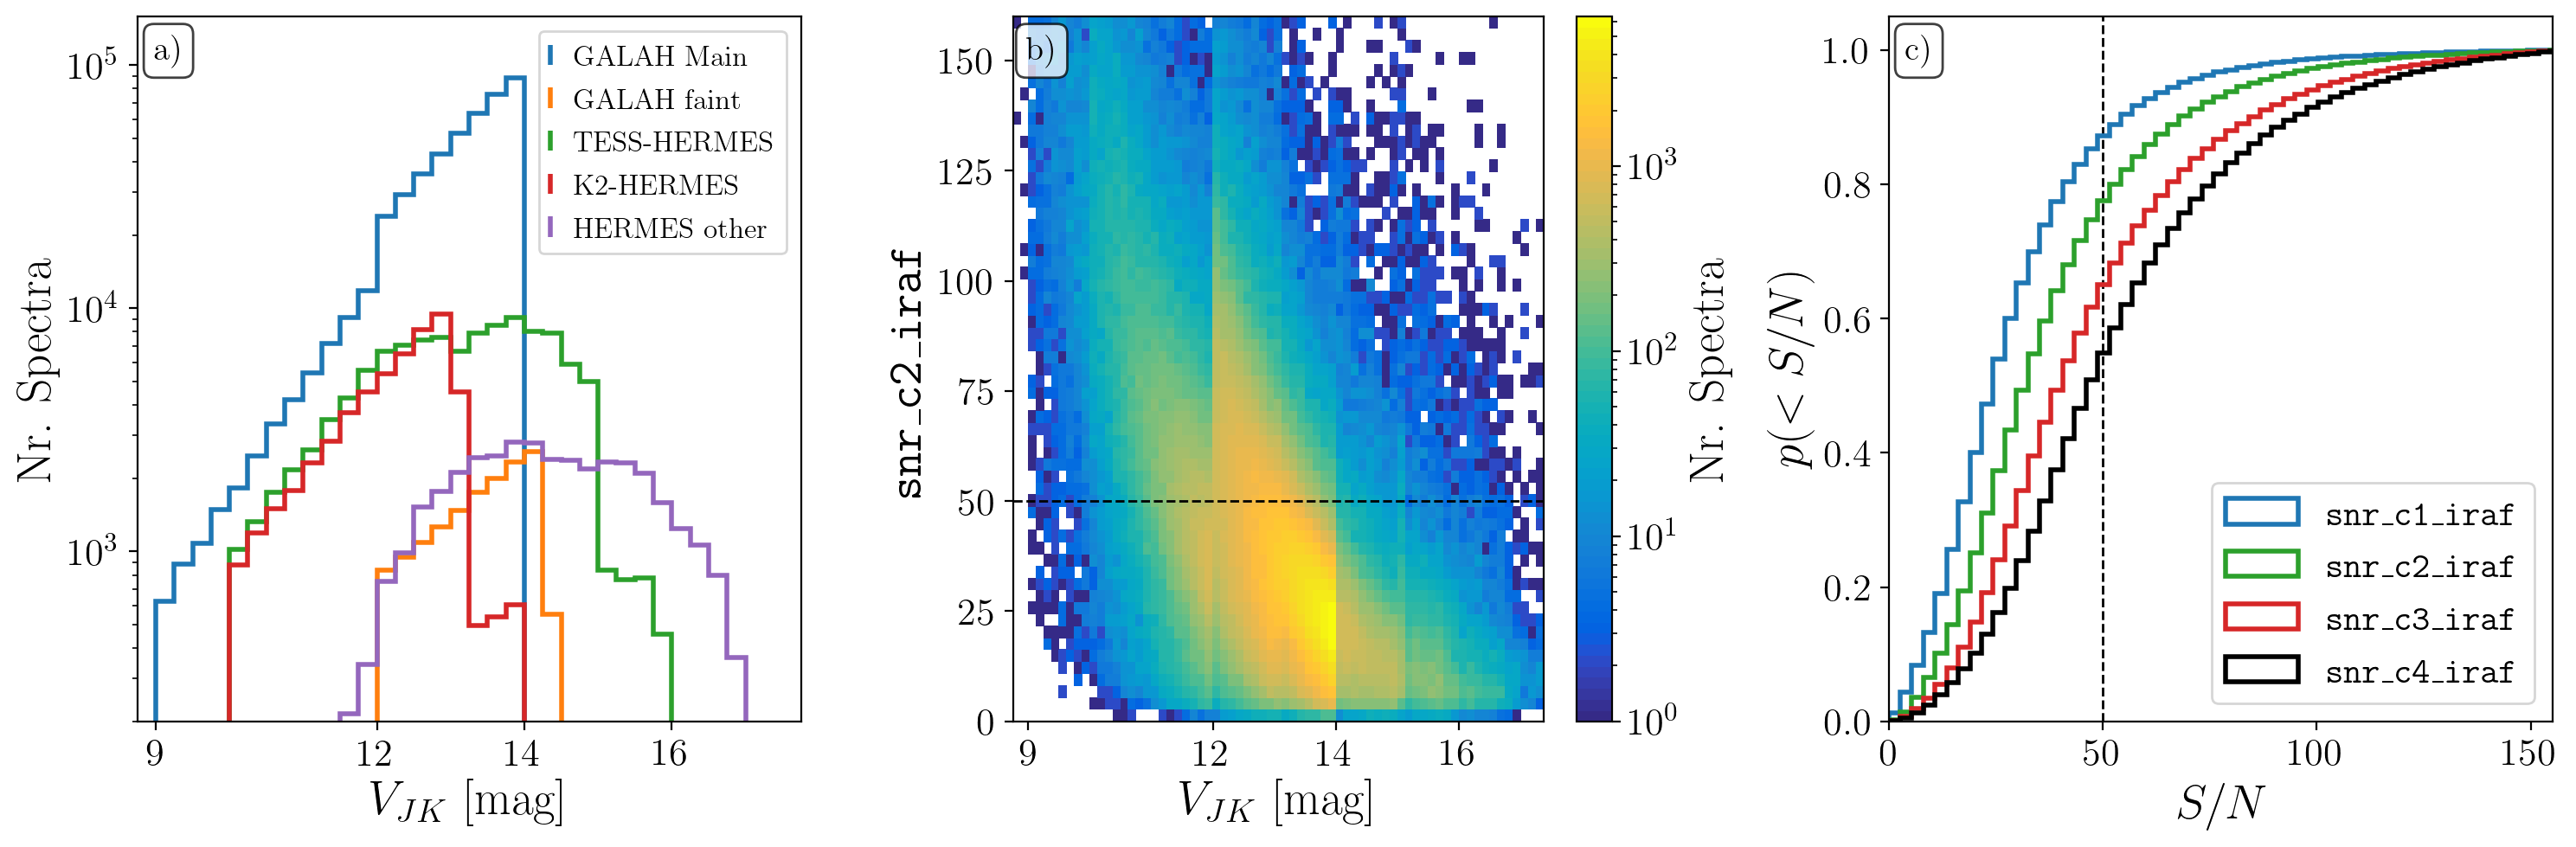
\includegraphics[width=\textwidth]{figures/hist_vjk_snr.png}
\caption{
\textbf{Distributions of magnitudes and $S/N$ of GALAH DR3.}
\textbf{Panel a)} Distribution of $V$ magnitude calculated from 2MASS $J$ and $K_S$.
\textbf{Panel b)} Distribution of average achieved $S/N$ per pixel for the green band (CCD 2) as a function of $V_{JK}$.
\textbf{Panel c)} Cumulative distribution of the $S/N$ per pixel of the different bands/CCDs of HERMES for GALAH DR3. A black, dashed line indicates the overall $S/N$ of 50 that we initially aimed for for CCD2.}
\label{fig:hist_vjk_snr}
\end{figure*}

Parallaxes are available from \Gaia\ DR2 for almost all stars observed by GALAH, and a vast majority of them are very precise, as can be seen in panel a) of Fig~\ref{fig:distance}. A total of 728651 are science observations of stars with matched \Gaia parallax measurements. $85\,\%$ (619~333) of them have a fractional parallax uncertainty below $10\,\%$. When dividing the sample into giants (\Teff$ < 5500\,\mathrm{K}$ and $M_{K_S} < 2\,\mathrm{mag}$) and dwarfs (\Teff$ \geq 5500\,\mathrm{K}$ or $M_{K_S} \geq 2\,\mathrm{mag}$), $93\,\%$ (454~406/488~192) of the observed dwarf stars have parallax uncertainties below $10\,\%$ and $69\,\%$ (164~927/240~459) of the observed giant stars have parallax uncertainties below $10\,\%$. The inferred distance estimates from \citet{BailerJones2018} are crucial for the small fraction of GALAH DR3 stars with parallax uncertainties above $20\,\%$.

Additionally, the available asteroseismic information is growing steadily as the analysis of data from the \Ktwo\ campaigns progresses. The overlap between GALAH targets and \Ktwo\ targets from campaign C1-C8 and C10-C13 has increased to almost 15,000 stars with measured asteroseismic $\nu_\mathrm{max}$ values and spectroscopic information and covers almost the entire red giant branch.

Since GALAH observes stars with fairly bright apparent magnitudes, almost all GALAH targets have well measured 5D information from \Gaia \citep{Brown2018, Lindegren2018}. An overview of the astrometric and spectroscopic quality for the observed stars can be found in Fig.~\ref{fig:distance}. The median fractional parallax error for GALAH stars is $2.7\,\%$, and $95\,\%$ of GALAH stars have parallax errors below $20\,\%$ (see panel a).

The magnitude limited selection of the GALAH survey (see the magnitude distribution in panel a) of Fig.~\ref{fig:hist_vjk_snr}) causes a strong correlation between increasing distance (and decreasing parallax quality) with increasing luminosity. This tradeoff between luminosity and parallax uncertainty was also visible for the stars in common between \Gaia DR1 and GALAH DR2 \citep{Buder2019} and is still present with the use of \Gaia DR2, as we illustrate in panel b) of Fig.~\ref{fig:distance} in Kiel diagrams, showing that especially giants with larger distances suffer from large parallax uncertainties.

\subsection{Observations}

GALAH data are acquired with the 3.9-metre Anglo-Australian Telescope at Siding Spring Observatory. Up to 392 stars can be observed simultaneously using the 2dF robotic fibre positioner \citep{Lewis2002} that sits at the telescope's prime focus. The fibres run to the High Efficiency and Resolution Multi-Element Spectrograph \citep[HERMES][]{DeSilva2015, Sheinis2015}, where the light is dispersed at $R\sim 28~000$ and captured in four independent cameras. HERMES records $\sim1000$~\AA\ of the optical spectrum across its four non-contiguous channels. Details of instrument design and as-built performance can be found in \citet{Barden2010}, \citet{Brzeski2011}, \citet{Heijmans2012}, \citet{Farrell2014} and \citet{Sheinis2015}.

Since the initial HERMES commissioning, the raw data has been contaminated by odd saturated points with vertical streaking, which was traced back to the choice of glass for the field flattening lens inside each of the four cameras \citep{Martell2017}. The original glass had been chosen for its high index of refraction, but uranium in the glass emitted $\upalpha$ particles that caused the saturated points and vertical readout streaks when they were captured by the HERMES CCDs \citep{Edgar2018}. In the first half of 2018, the original field flattening lenses were replaced with lenses made from a less radioactive glass, and the vertical streaks have almost stopped occurring in the data. The point spread function in the HERMES cameras changed as a result of changing the field flattening lenses, and is now larger and less symmetric in the corners of the detectors. As part of HERMES recommissioning, the GALAH team fed light from a Fabry-Perot interferometer into HERMES to characterise the new PSF across each detector, and this information has been incorporated into the data reduction procedure.

The observing procedure and targeting strategy for this data release are the same as for previous public GALAH data, including the selection of fields via $\texttt{obsmanager}$ and the assignment of targets onto 2dF fibres via $\texttt{configure}$ \citep{Miszalski2006}. For further information on the strategy of GALAH Phase 1, with the GALAH main and GALAH faint observations, we refer the reader to \citet{Buder2018}. For the K2-HERMES observing strategy, the reader is referred to \citet{Wittenmyer2018, Sharma2019} and for TESS-HERMES to \citet{Sharma2018}.

GALAH DR3 is a significant increase in the number of targets relative to DR2, and includes data taken between November 2013 and February 2019. The distribution of GALAH DR3 stars across $V_{JK}$ and signal-to-noise ratio (S/N) is shown in panel b) Figure \ref{fig:hist_vjk_snr} and adds another perspective on the complex correlation of luminosity (or surface gravity $\log g$) with $S/N$ for the observed stars, which is shown in panel c) of Fig.~\ref{fig:distance}.

GALAH, \Ktwo-HERMES, and \tess-HERMES observers choose from a database of available fields depending on conditions, limiting the hour angle to within $\pm 2$ hours whenever possible. The standard observing procedure for regular GALAH survey fields is to take three 1200s exposures, with an arc lamp and flat lamp exposure taken at the same sky position as each field to enable proper extraction and calibration of the data. Bright-star fields are observed in evening and morning twilight, and in case of seeing too poor for the regular survey fields. They receive three 360s exposures and the same calibration frames.

The median seeing at the AAT is $1\farcs 5$, and the exposure time is extended by $33\,\%$ if the seeing is between $2\farcs 0$ and $2\farcs 5$ and by $100\,\%$ if the seeing is between $2\farcs 5$ and $3\farcs 0$. This exposure time was chosen to return a S/N of 50 per pixel (equivalent to 100 per resolution element) in the HERMES green channel (CCD 2).  This is accomplished in nominal seeing when a star has an apparent magnitude of 14 in the photometric band matched to the camera (B=14 and CCD 1, V=14 and CCD 2, etc.) Mismatches between predicted and actual data quality are due to a combination of seeing, cloud, inaccuracy in $V_{JK}$, and the nonzero colours of stars (i.e., a hot star will be brighter in the blue and green passbands and fainter in the red and infrared passbands, and its S/N will vary accordingly). We show the distribution for the actual S/N per pixel as a function of $V_{JK}$ in panel b) of Fig.~\ref{fig:hist_vjk_snr}, and a cumulative distribution for all four HERMES channels in panel (c) of the same Figure. 

\subsection{Reductions}\label{sec:reductions}

Since GALAH DR2 we have improved our reduction pipeline \citet{Kos2017}, and all spectra icluded in DR3 have been reduced again. As in GALAH DR2, raw images are corrected for bias level and flat field, and cosmic rays are removed with a modified LaCosmic algorithm \citet{vandokkum2001}. Scattered light and fibre-cross talk signals are removed. The wavelength solution for the extracted spectra is found via fitting of ThXe arc lamp observations. Sky spectra are modelled from the 25 sky fibres included in each field and subtracted, and synthetic telluric lines are computed using \texttt{molecfit} \citep{Kausch2015, Smette2015} and removed from observed spectra. The reduction pipeline runs a cross-correlation with \texttt{AMBRE} spectra \citep{DeLaverny2012} to provide a first estimate of stellar parameters \Teff, \logg, \feh, and \vrad,   and to normalise the spectra.

The main improvement is the wavelength solution, which is now more stable at the edges of green and red CCDs, where we lack arc lines. This has been achieved by monitoring the solution and fixing the polynomial describing the pixel-to-wavelength transformation, if deviations from a typical or average solution are detected. The solution is described by a 4th order Chebyshev polynomial. We are using \textsc{IRAF}'s \texttt{identify} function to find positions of arc lines in each image and match them with our linelist. Fitting the solution, however, is now done in a more elaborate way. Initially, all spectra from the same image are allowed to have an independent solution. Then the four coefficients of the Chebyshev polynomial are compared. The first coefficient defines the zero-point. Because the 2dF fibres are not arranged monotonically in the pseudo-slit, the first coefficient is truly independent of the spectrum number (spectra being numbered 1 to 400 in each image). The values of the other three coefficients should be a smooth function of the spectrum number. If a coefficient for a specific spectrum deviates by more than $3\upsigma$ from a smooth function, it is corrected to lie on the smooth function. This successfully fixes the previous problems with incorrect wavelength solutions at the edge of the image. 

Cross-talk is now parametrized differently. It can only be measured in larger gaps between every 10th spectrum. Cross-talk was previously represented as a function of the position in the image, but now each batch of 10 spectra (from one slitlet) is assigned the measured cross-talk without any interpolation. The cross-talk is still a function of the direction along the dispersion axis. The normalisation has been improved with a new identification of continuum sections (regions of a spectrum where the continuum is measured) and optimised polynomial orders. 

The pipeline has been actively maintained and adapted to perform well with the recommissioned instrument %(major modification was replacement of some radioactive glass -- there are now fewer cosmic rays, but the image is more distorted in the corners). 
following the replacement of the field flattening lenses in 2018 May. Other minor improvements and computing optimisations have been made.

%________________________________________________________________
\section{Data analysis} \label{sec:analysis}

In this section we describe how the outputs from the data reduction process, delivered by WG3, are used to estimate final stellar parameters for each spectrum as well as up to 30 element abundances. As described in Section \ref{sec:reductions}, WG3 generates reduced spectra, initial estimates of radial velocity \vrad, and \vrad-shifted, normalised spectra, as well as initial estimates of the stellar parameters \Teff, \logg, and \feh. 

\paragraph*{Changes from GALAH DR2 to GALAH DR3:} The most important difference to the workflow of our analysis is that we do not use data-driven approaches for the spectrum analysis in GALAH DR3, but only the spectrum synthesis code Spectroscopy Made Easy \citep[][hereafter {\textsc{sme}}]{Valenti1996, Piskunov2017}, which had only been used for the training set analysis in DR2. We visualise the reasons for this step with the comparison of GALAH DR2 and DR3 in Fig.~\ref{fig:galah_dr3_comparison_dr2}. We found in DR2 that stars at the periphery in stellar label space, e.g. high temperature (compare panels a) and d) or low metallicity (compare panels b) and e)) did not receive optimal labels from the data driven process.  
Possible reasons for this are the limited flexibility of the quadratic model that was used, gradient aliasing, and the underrepresentation of these stars in the training set. The latter was also an important factor for the limited number of unflagged abundance measurements. As a result, we had to flag those labels as unreliable in the data release. The flagged results are shown as the lighter blue background in Fig.~\ref{fig:galah_dr3_comparison_dr2}, where it can be clearly seen in panel a) that some of the inferred stellar parameters are unphysical, as in the upturn in the low-mass main sequence and the correlation between \Teff and \logg for hot stars. The effect of flagging on the inferred stellar abundances can best be seen in the drastic increase in Li detections in DR3 (compare panels c) and f)), which was limited to warm dwarfs and Li-rich giants in DR2 due to the selection of training set stars. \KL{These explanations are missing the point that the morphology of the CMD looks much better in DR3 because astrometric constraints were used in addition to spectroscopy. Data-driven methods combined with such constraints may perform equally well. Also, the much fewer Li-detections in DR2 had to do also with more strict limits for what counted as detections and the lack of RV-flexibility.}

Being able to estimate reliable stellar parameters for hot stars (see panel d) has also enabled the determination of several of their abundance patterns, which was not possible in DR2. Intriguingly, some of the A- and F-type main sequence stars exhibit under-abundant [$\upalpha$/Fe] (see lowest measurements in panel e) and overabundant iron-peak and neutron-capture elements, which is the peculiar chemical compositions of Am/Fm stars \citep[see e.g.][]{Xiang2020}. In DR3, we are also able to estimate more accurate element abundances for metal-poor stars, in particular those with the previously identified low-$\upalpha$\footnote{These stars have lower abundances in the $\upalpha$-elements when compared to the high-$\upalpha$ disk population.} ``outer'' halo pattern \citep[see e.g.][]{Nissen2010}.

% This figure was created with the notebook GALAH_DR3/validation/comparisons/comparison_galah_dr2/galah_dr3_comparison_dr2.ipynb
\begin{figure*}
\centering
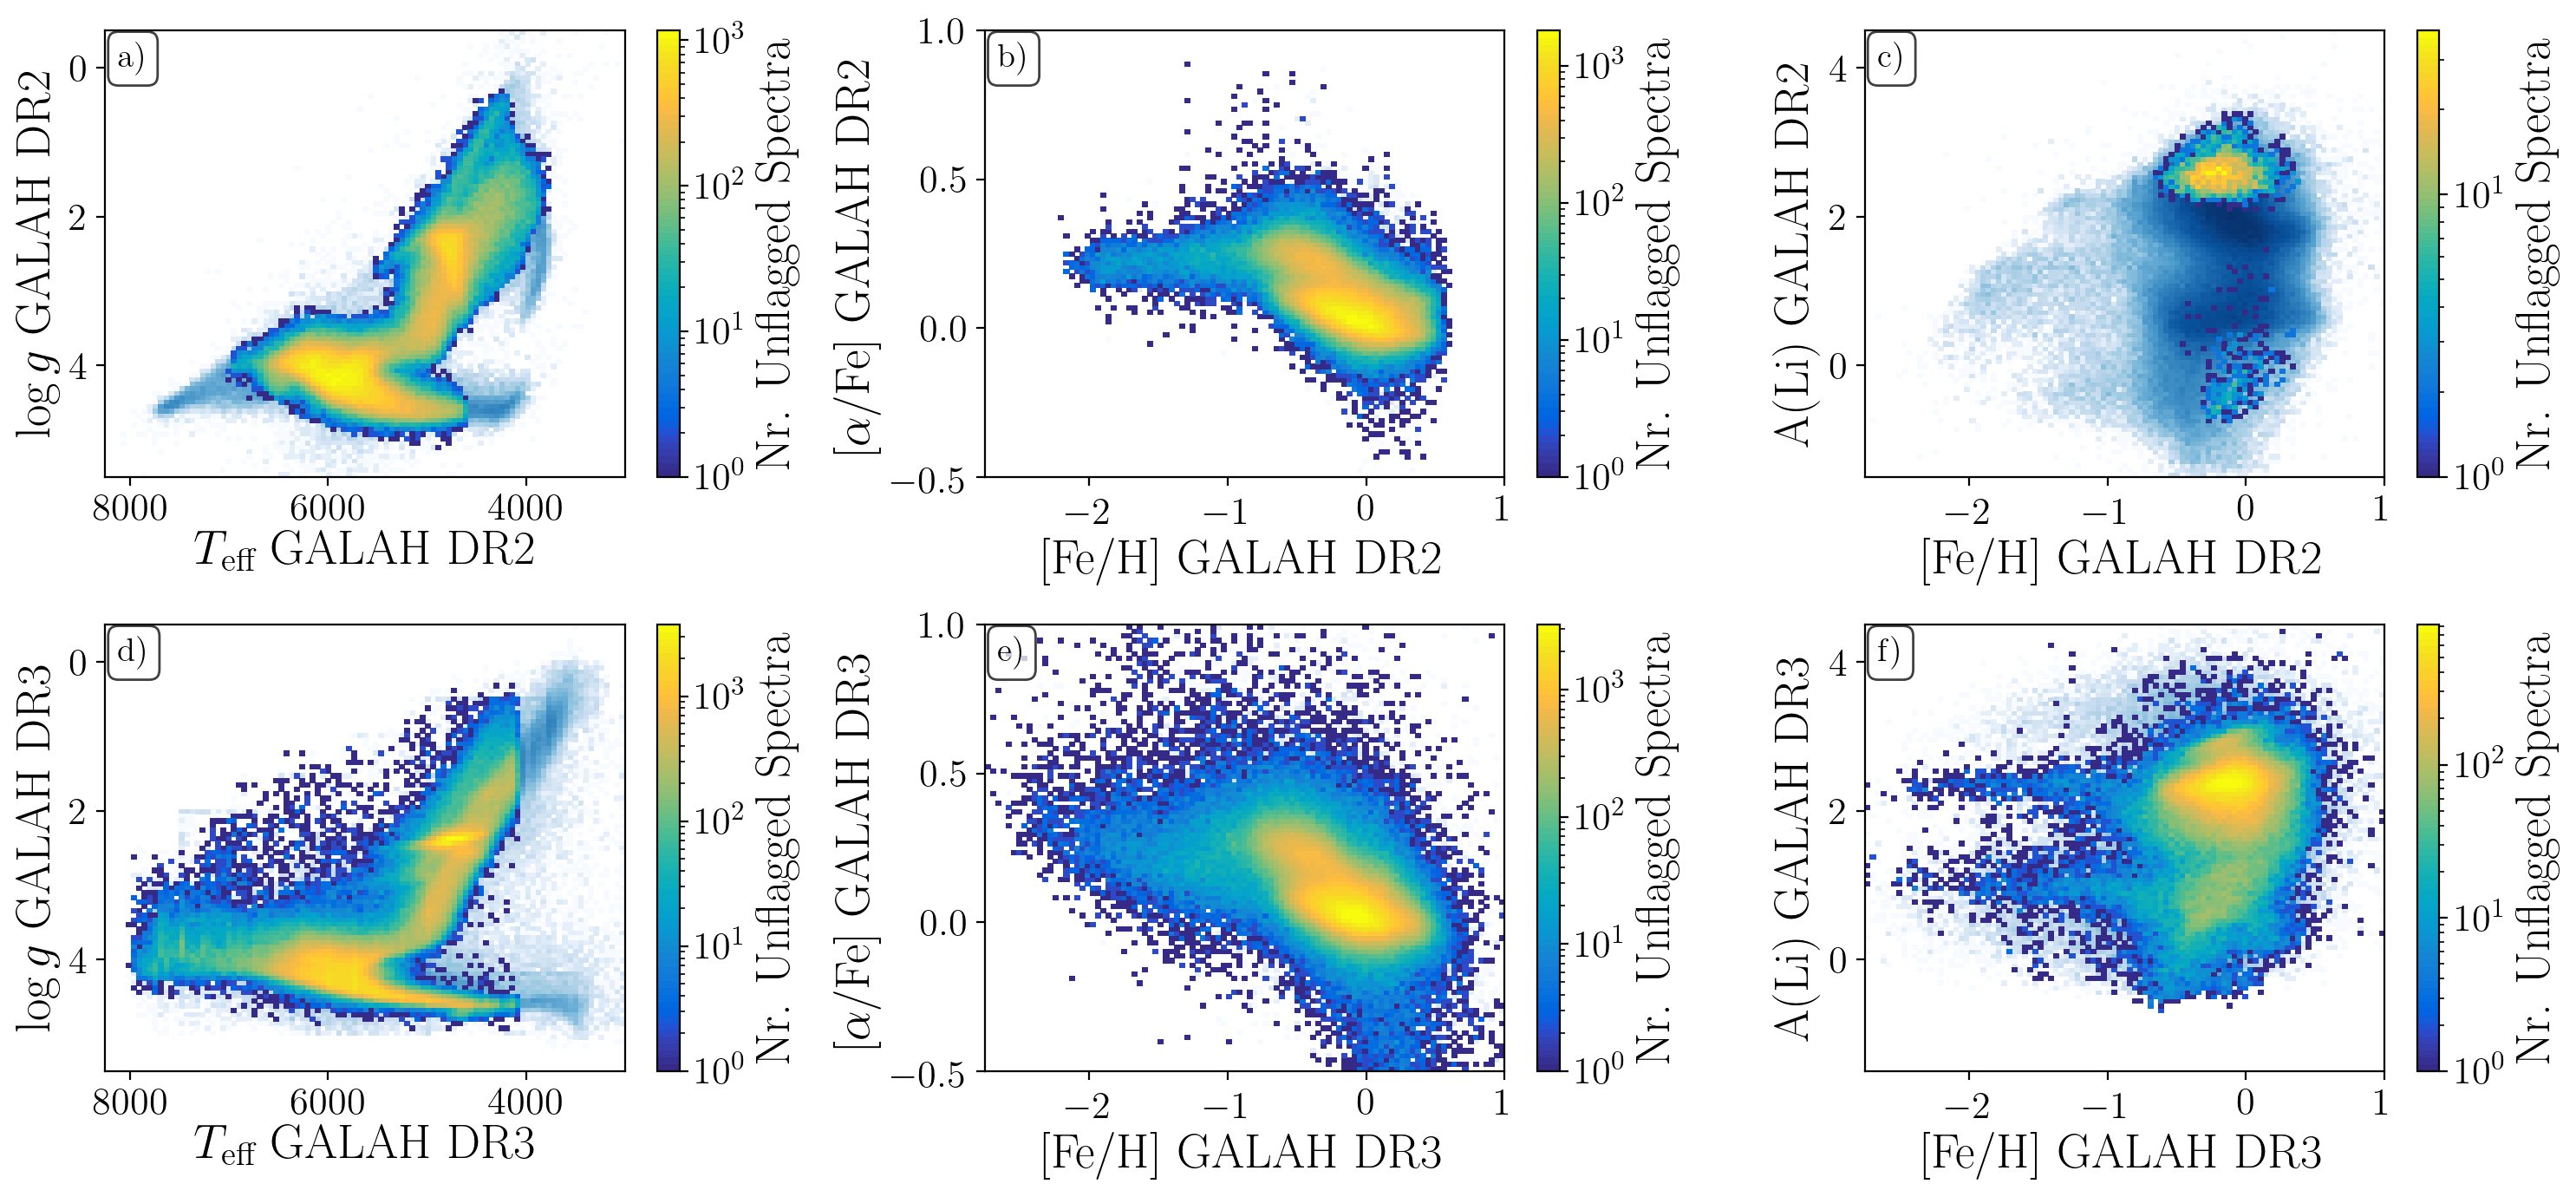
\includegraphics[width=\textwidth]{figures/galah_dr3_comparison_dr2.png}
\caption{
\textbf{Comparison of GALAH DR2 (upper panels) and GALAH DR3 (lower panels, this release).}
The smooth light blue background indicates all measurements, whereas the colormap shows the number of unflagged measurements at each point. \textbf{Left panels:} Kiel diagrams, i.e. \Teff versus \logg, for stars of DR2 \textbf{(a)} and DR3 \textbf{(d)}. \textbf{Middle panels:} Abundance pattern of iron vs. $\upalpha$-process elements, i.e. \feh versus \alphafe, for DR2 \textbf{(b)} and DR3 \textbf{(e)}. \textbf{Right panels: } Absolute Li abundance as a function of iron abundance, i.e. \feh versus A(Li), for DR2 \textbf{(c)} and DR3 \textbf{(f)}. The stellar parameters and abundances from GALAH DR2 appear more tightly constrained, but we note that this is an artefact of the data-driven approach, which tends to find solutions closer to the mean parameter/abundance patterns. We include all DR2 and DR3 stars in these panels, and not just the stars common to both to highlight the increase in accuracy of stellar parameters and coverage of abundances, rather than the improvement change in precision for the same spectra.}
\label{fig:galah_dr3_comparison_dr2}
\end{figure*}

For this data release, we only run the analysis pipeline for spectra of stars that can estimate reasonable initial radial velocities (either as part of previous GALAH runs, the reduction pipeline or from Gaussian fits to the Balmer lines) and have external information on parallaxes from \Gaia \citep{Lindegren2018}. \KL{How many stars does this exclude?}. For a few bright stars that are not in \Gaia DR2, we take parallax from \Hipparcos \citep{vanLeeuwen2007}.

\paragraph*{The general workflow} of the analysis of spectra as part of this data release has thus been adjusted to the following (with more details given hereafter). \KL{Can the section be structured better? Following the bullet list, items are listed in somewhat arbitrary order. A few introductory sentences should be included to explain the structure and the overall goal, i.e. homogeneously and automatically analyse a large number of spectra that intrinsically look very different. This brings challenges on technical and physical aspects.}:
\begin{enumerate}
\item Initialise {\sc sme} (version 536) with choices of line data, atmosphere grid, non-LTE departure grids, observed spectrum (limited to the 46 segments used for the parameter estimation) including selection of continuum and line masks, initial parameters for $\chi^2$ optimisation. Check if all external information is provided and then update the initial \logg with this external information and the initial stellar parameters as outlined in the explanation of surface gravities.
\item Normalise all 46 segments individually with the chosen initial setup by fitting linear functions first to the observed spectrum and then to the difference of the observed and synthetic spectrum.
\item Optimise the stellar parameters \Teff, \feh, \vbroad (\vsini with \vmac set to 0), and global \vrad with 2 major {\sc sme} update loops (calculating double-sided partial derivatives and exploring the local $\chi^2$ surface with up to 5 different parameter choices). Consistently update \logg and \vmic from physical and empirical relations, respectively, with every change of \Teff or \feh. In our test, this already led to updated parameters close to the $\chi^2$ global minima.
\item Normalise all 46 segments again individually as in step 2, but with updated stellar parameters.
\item Optimise the stellar parameters \Teff, \feh, \vbroad, and \vrad with up to 20 major {\sc sme} update loops as in step 3 until fractional change of $\chi^2$ is below 0.001. Because of the resolution of GALAH, \vsini and \vmac are degenerate broadening influences and we thus fit them with {\sc sme} by setting \vmac to 0 and only fit \vsini \KL{This description of vsini and vmac can be moved up to where vbroad is first mentioned}.
\item Collect stellar parameters for validation. Save covariance uncertainties, based on the statistical $\chi^2$ uncertainties given the uncertainties of the normalized flux, in addition to the uncertainties delivered by {\sc sme} version 536 \citep[see][for more details]{Piskunov2017}. The validation of stellar parameters (see Sec.\ref{sec:validation_sp}), led to an adjustment of the estimated atmospheric [Fe/H] ({\sc sme}.feh) by adding $0.1\,\mathrm{dex}$\footnote{This is not the final $\mathrm{[Fe/H]} = \textsc{fe\_h}$ as reported in this data release, but a pseudo iron abundance $\textsc{sme}.\mathrm{feh} = \textsc{fe\_h\_atmo}$, estimated from H, Sc, Ti, and Fe lines.}.
\item Initialise {\sc sme} (version 536) for the element abundance estimation with choices of line data, atmosphere grid, non-LTE departure grids, observed spectrum (limited to line segement(s) used for the element abundance estimation) including selection of continuum and line masks, final global atmosphere parameters for $\chi^2$ optimisation. Contrary to steps 3 and 5, hereafter the aforementioned global parameters, including \vrad, are kept fixed\footnote{We note though, that we have performed a test of the reliability of the Li line measurement by also allowing a local \vrad fit to overcome shortcomings of the wavelength solution of the red CCD 3.}.
\item Normalise all segments for the line (e.g. Li6708) or element (e.g. Ca) run individually with the chosen initial setup by fitting linear functions first to the observed spectrum. Improve this normalisation by fitting a linear function to the difference between the observed and synthetic spectrum to create a 'full' synthetic spectrum.
\item \KL{Explain why, i.e. the same line has a different degree of blending in different stars.} Create a 'clean' synthetic spectrum only based on the lines of the element to be fitted. Then compare the 'full' and 'clean' spectra for the chosen line mask pixels and neglect those which deviate more than \KL{$\Delta\chi^2>0.005$} for elements other than Fe.
\item Optimise the relevant element abundance entry in the abundance table ({\sc sme}.abund) with up to 20 major {\sc sme} update loops until fractional change of $\chi^2$ is below 0.001. The atmosphere is updated with each change of chemical composition to stay consistent, but we note that for the sake of computation cost with {\sc sme}, the abundances, that are not fitted, are kept at scaled-solar, with the exception of Li with A(Li) = 2.3, an enhancement of $0.4\,\mathrm{fex}$ for N, and the precomputed $\upalpha$-enhancement for $\upalpha$-process elements.
\item Collect stellar parameters and element abundances for validation and post-processing.
\item Calculate upper limits for each element/line for non-detections by estimating lowest abundance would lead to a line flux depression of 0.03 below normalised continuum (see more detailed explanations below).
\item Post-processing: apply flagging algorithms, calculate final uncertainties from accuracy and precision estimates, combine line-by-line measurements of element abundances weighted by their uncertainties.
\end{enumerate}

\paragraph*{The line data} is based on the corresponding compilation for the Gaia-ESO survey \citet{Heiter2015b, Heiter2020} with few \KL{Will check is few is a good summary} updated $\log gf$ values. The final compilation of the used lines for stellar parameter and element abundance estimation together with the most important line data is listed in Table~\ref{tab:linelist}.

\paragraph*{The segments and masks for stellar parameter estimation} are based on selected neutral and ionised Sc, Ti, and Fe lines as well as the two Balmer lines $\mathrm{H_\alpha}$ and $\mathrm{H_\beta}$. We chose these lines based on their experimental or theoretical line data quality and limit ourselves to the least blended lines or parts of lines. The masks used for parameter and abundance optimisation were selected based on the line shapes of several thousand randomly selected spectra (including those of crowded cool stars with dominant molecular absorption bands). The masks used for continuum placement were selected on-the-fly as the regions with smallest amount of line absorption, ensuring a sufficient number of (pseudo-)continuum points on either side of the line mask is ensured.

\paragraph*{The model atmospheres} are theoretical 1D hydrostatic ones from {\sc marcs2014} grid \citep{Gustafsson2008}.  The adopted grid is the same as in GALAH DR2 \citep[][Sect. 3.2]{Buder2018}. In brief, they cover $2500 \leq T_\mathrm{eff} \leq 8000\,\mathrm{K}$, $-0.5 \leq \log g \leq 5.5\,\mathrm{dex}$ with the exclusion of the hottest and lowest surface gravity regions, $-5 \leq \mathrm{[Fe/H]} \leq 1$, and were computed with the solar chemical composition of \citet{Grevesse2007}, scaled by [Fe/H] and with $\upalpha$-enhancements as laid out later in this section. Plane-parallel models were adopted for $\log g \geq 4$, and spherically-symmetric models for $\log g \geq 3.5$.

\paragraph*{The non-LTE grids} of departure coefficients, that we use for the on-the-fly synthesis of 1D NLTE spectra are described in \citet{Amarsi2020}. In brief, new grids of departure coefficients were constructed by adopting the non-LTE model atoms presented for H \citep{Amarsi2018}, Li \citep[][Wang et al., in prep]{Lind2009}, C \citep{Amarsi2019}, O \citep{Amarsi2018b}, Na \citep{Lind2011}, Mg \citep{Osorio2015}, Al \citep{Nordlander2017}, Si \citep{Amarsi2017}, K \citep{Reggiani2019}, Ca \citep{Osorio2019}, Mn \citep{Bergemann2019b}, and Ba \citep{Gallagher2020}, and running on the {\sc marcs} model atmosphere grid using the non-LTE radiative transfer code {\sc balder} \citep{Amarsi2018}, a modified version of {\sc multi3d} \citep{Leenaarts2009}.  For Fe, the same non-LTE grids of departure coefficients that were used in GALAH DR2 were adopted here \citep{Amarsi2016a, Lind2017}.  We want to stress that this approach is different to many other major surveys like APOGEE \citep{SDSSDR16}, RAVE \citep{Steinmetz2020b}, and Gaia-ESO \citep{Smiljanic2014}, who only report 1D LTE results in their public data releases. \SB{CHECK IF THAT IS STILL TRUE}.

\paragraph*{Initial stellar parameters and abundances} are chosen depending on the quality of reduction products and their availability in GALAH DR2 \citep{Buder2018}. If the stellar parameters of GALAH DR2 (and non-published spectra of K2-HERMES, TESS-HERMES and other spectra analysed in the same way via \textit{The Cannon}) are not flagged, we use those. Otherwise we use initial rough stellar parameters provided as part of the reduction pipeline as part of its radial velocity estimation with grid interpolation, if they are unflagged. Otherwise we use a set of fiducial stellar parameters ($T_\text{eff} = 5500\,\mathrm{K}$, $\log g = 3.0\,\mathrm{K}$, and $\mathrm{[Fe/H]} = -0.5\,\mathrm{dex}$ as well as the result of Gaussian fits to the two Balmer lines for \vrad). We initialise the abundance pattern as scaled-solar, but adjust the alpha-enhancement as described later in this section.

\paragraph*{Surface gravities} are updated self-consistently with the other stellar parameters for each synthesis step via the fundamental relation of \logg, stellar mass $\mathcal{M}$, and bolometric luminosity $L_\text{bol}$
\begin{equation}
\log \frac{g}{g_\odot} = \log g_\odot + \log \frac{\mathcal{M}}{\mathcal{M_\odot}} + 4 \log \frac{T_\mathrm{eff}}{T_\mathrm{eff,\odot}} - \log \frac{L_\mathrm{bol}}{L_\mathrm{bol,\odot}} \label{eq:logg}
\end{equation}

\paragraph*{Bolometric luminosities} are estimated via
\begin{equation}
\log \frac{L_\mathrm{bol}}{L_\mathrm{bol,\odot}} = -0.4 \cdot \left(K_S - 5\cdot \log \frac{D_\varpi}{10} + BC(K_S) - A(K_S) - M_{bol,\odot} \right) \label{eq:lbol}
\end{equation}
from the 2MASS \citep{Skrutskie2006} $K_S$ band, a consistently calculated bolometric correction $BC(K_S)$ for this band using stellar parameters for each synthesis step, distances $D_\varpi = \texttt{r\_est}$ from \citet{BailerJones2018} as well as extinctions $A_{K_S}$ in the $K_S$ band. If both 2MASS $H$ \citep{Skrutskie2006} and WISE $W2$ \citep{Cutri2013} band information were having quality A we used the RJCE method \citep{Majewski2011} to compute $A_{K_S}  = 0.917 \cdot \left( H - W2 - 0.08 \right)$ and thus only in a few cases via $A_{K_S} = 0.38 \cdot \texttt{E(B-V)}$ \citep{Savage1979}.

\paragraph*{Bolometric corrections} are estimated consistently by interpolation of the grids from \citet{Casagrande2014, Casagrande2018} using stellar parameters for each synthesis step in combination with the extinction provided by the maps of \citet{Schlegel1998} up to $E(B-V) < 0.48$.

\paragraph*{Stellar masses} are needed to estimate the surface gravities according to Eq.~\ref{eq:logg}, but also depend on the surface gravity, luminosities or absolute magnitudes, if estimated via isochrone interpolation. We therefore estimate them iteratively and self-consistently together with $\log g$ via isochrone interpolation whenever a stellar parameter $O_i \in$ [\Teff, \logg, \feh, and \lbol] is updated during the parameter optimisation. We assume that these parameters have Gaussian uncertainties and no covariances. This is a bold assumption, given that we use both \logg and \lbol, which convey very similar information. However, we use large uncertainties for \logg, to limit its influence to extreme cases and can then write
\begin{equation}
\mathcal{L} \sim \prod_i \frac{1}{\sqrt{2 \pi} \sigma_i} \cdot \exp \left( - \frac{\left( O_i - S_i \right)^2}{2 \sigma_i^2} \right)
\end{equation}

Because we do not have final uncertainties for the stars at hand, we assume that the parameter uncertainties $\sigma_i$ are $100\,\mathrm{K}$, $0.5\,\mathrm{dex}$, $0.2\,\mathrm{dex}$, and $0.1\cdot L_\text{bol}$ for \Teff, \logg, \feh, and \lbol, respectively. We want to stress that these are not the final average uncertainties, but these values were chosen after extensive tests of ensuring enough isochrone points to be considered for the mass interpolation within the uncertainties. For the final uncertainties of this release, we use a more sophisticated implementation (see Sec.~\ref{sec:validation_sp}). We convert the iron abundances into a measurement of metallicity $Z$ by assuming the $\upalpha$ enhancement to follow the stellar parameter relation layed out later in this section and combine this $\mathrm{[\upalpha/Fe]}$ and the atmospheric iron abundance to [M/H] via the correlation by \citet{Salaris2005} and into $Z$ with the Solar value from the {\sc parsec+colibri} isochrones \citep{Bressan2012, Marigo2017}. We then use these {\sc parsec+colibri} isochrones on a grid with ages of $0.5...(0.5)...13.5\,\mathrm{Gyr}$ and $\mathrm{[Fe/H]} = -2.4...(0.1)...0.6\,\mathrm{dex}$. to estimate maximum likelihood masses on-the-fly.

\paragraph*{Microturbulence velocities} $v_\mathrm{mic} = \texttt{vmic}$ were computed consistently from the empirical relations estimated for the GALAH survey, that is,
\KL{Put c1 and c2 on separate rows beneath the expression.}
\begin{equation}
v_\mathrm{mic} = 1.1 + c_1 \cdot (T_\mathrm{eff}-5500\,\mathrm{K}) + c_2 \cdot (T_\mathrm{eff}-5500\,\mathrm{K})^2,
\end{equation}
with $c_1 =1.6 \cdot 10^{-4}$ and $c_2 = 0$ for cool main sequence stars ($T_\mathrm{eff} \leq 5500\,\mathrm{K}$ and $\log g \geq 4.2\,\mathrm{dex}$) and $c_1 =1.0 \cdot 10^{-4}$ and $c_2 = 4 \cdot 10^{-7}$ for evolved and hotter stars ($T_\textrm{eff} \geq 5500\,\mathrm{K}$ and $\log g \leq 4.2\,\mathrm{dex}$), where \vmic is given in $\mathrm{km\,s^{-1}}$. We elaborate in Sec.~\ref{sec:caveats} on possible systematic trends that this simplified function could introduce.

\paragraph*{Element abundances} are computed during the analysis with the {\sc sme}-internal notation of relative abundances for the first 99 elements, such that their sum amounts to 1. These are initialised consistently with the {\sc marcs} pattern from the Solar abundances of \citet{Grevesse2007}. This notation is different from the usual $A(\mathrm{X}) = \texttt{A\_x} = \log \epsilon (\mathrm{X})$ and we thus convert them when readings out the final abundance pattern. In our final notations of element X, we report $A(\mathrm{X})$ on the customary astronomical scale for logarithmic abundances, where H is defined to be $\log \mathrm{H} = 12.00$, that is, $A(\mathrm{X})= \log \frac{N_\mathrm{X}}{N_\mathrm{H}} + 12$, where $N_\mathrm{X}$ and $N_\mathrm{H}$ are the number densities of elements X and H, respectively. We further report relative abundances as $\mathrm{[X/H]} = A(\mathrm{X}) - A(\mathrm{X})_\odot$ and $\mathrm{[X/Fe]} = \mathrm{[X/H]} - \mathrm{[Fe/H]}$. For the explanation of our chosen values of $A(\mathrm{X})_\odot$ see Sec.~\ref{sec:accuracy_abundances} and for their values see Tab.~\ref{tab:solar_reference_values2}. This table also lists the lines used for the line-by-line analysis, which were later combined for the final element abundances reported as {\sc x\_fe} for element X.

\begin{figure*}
\centering
\includegraphics[width=\textwidth]{figures/old/Si_compilation.pdf}
\caption{
\textbf{Comparison of abundance trends for different Si lines in the course of selecting reasonable Si lines for the final GALAH computations.}
\textbf{Top left panel:} Final combination of all Si I lines for our test subset. \textbf{Other panels: } Abundance trends for individual lines (wavelengths indicated in the bottom left of each panel). Black lines indicate a global solar value of $A(\mathrm{Si})_\odot = 7.51$. Black dotted lines indicate the best fit to the sky flat for each line, thus indicating differences in the accuracy of abundances (with the least accurate line being Si 5666). Differences in the overall shape of the abundance trends indicate different precisions or issues with blending or line strength (e.g. Si6722 with many high [Si6722/Fe] estimates compared to the other lines.)
}
\label{fig:Si_abundance_zeropoint_differences}
\end{figure*}

\paragraph*{Line-by-line vs. combined abundance analysis} was selected based on the time and computation resources available. Due to the ongoing improvements of line selections and non-LTE grids during the analysis of GALAH DR3, we needed to run the elements with 1D non-LTE results (Li, C, O, Na, Mg, Al, Si, K, Ca, Mn, Fe, Ba) as well as Cr and Sc with all lines of the element simultaneously rather than line-by-line. During the development of the pipeline we have tested all individual lines for the elements run with non-LTE and only selected those with similar trends and absolute abundances to run combined. By using individual lines, we are less prone to unreliable line data, such as unreliable $\log gf$ values. Wrong oscillator strengths introduce a bias in the absolute abundance for each line (see for example our tests for a comparison of different line estimates of Si in Fig.~\ref{fig:Si_abundance_zeropoint_differences}). The Si lines at $5666\,\mathrm{\AA}$ is for example less accurate than the rest of the lines, because the oscillator strength that was measured in the laboratory \citep{GARZ,BL} is contaminated by a theoretically estimated lines by \citet{K07}. When such a line would be used for a global synthetic fit of [Si/Fe], they would introduce both a bias in the final abundance and parameter- as well as $S/N$-depending systematic trends. When the Solar abundance for these lines are however estimated independently from the others, they can still be used for the combined [Si/Fe] abundance, after applying individual Sun-based corrections to the absolute abundances. This line was thus neglected for the final combined fit of [Si/Fe] similarly to the less precise lines like Si6722 or Si7680, where a large number of overestimated Si abundances due to blending or wavelength calibration issues would have contaminated the final measurement. \KL{This section is a bit confusing. Si is a NLTE element and was not run line by line. But we compared the line approach with the combined for these elements and I don't recall a big difference. Maybe I am forgetting something. Anyway, it is important that the reader understands that NLTE in itself did not affect computational time. }

\paragraph*{Alpha-enhancement $\mathrm{[\upalpha/Fe]}$} is treated differently during the stellar parameter on the one side and element abundance iteration of alpha-element on the other. In all cases, we initialise the abundances with the scaled-solar pattern. We then adjust the alpha-enhancement for the elements O, Ne, Mg, Si, S, Ar, Ca, and Ti with the common enhancement pattern of $\mathrm{[\upalpha/Fe]} = 0.4\,\mathrm{dex}$ for $\mathrm{[Fe/H]} \leq -1.0\,\mathrm{dex}$ as well as $\mathrm{[\upalpha/Fe]} = 0.0\,\mathrm{dex}$ for $\mathrm{[Fe/H]} \geq 0.0\,\mathrm{dex}$ and a linear function between both iron abundances. We update this value consistently whenever [Fe/H] changes. For the individual lines of O, Mg, Si, Ca, and Ti as part of GALAH DR3, we then update their actual abundances while keeping the other abundances fixed. The final reported global $\mathrm{[\upalpha/Fe]} = \texttt{alpha\_fe}$ is then an error-weighted combination of selected Mg, Si, Ca, and Ti lines (Mg5711, Si, Ca, Ti4758, Ti4759, Ti4782, Ti4802, Ti4820, and Ti5739). We stress however, that this combination is depending on the detection of these lines and might come down to a single measurement, whereas other estimates are a combination of up to 9 measurements (Mg5711, Si, Ca, Ti4758, Ti4759, Ti4782, Ti4802, Ti4820, and Ti5739). We also want to stress that this approach is different from the estimation from APOGEE (with an overall averaged ratio for alpha-process elements in the synthetic spectra) or simple averages of the element abundances.\KL{Can all comparison, favourable and not, between GALAH analysis techniques to APOGEE and other surveys techniques be put in one section? It does not read so nicely to encounter arguments like these throughout the text.}

\paragraph*{Upper limits} are calculated for all measured lines/elements if no detection was possible. In this case we estimate the smallest abundance needed to explain a line strength, that is the difference of line to continuum flux in the normalised spectrum of at least 0.03 or at least $1.5/(S/N)$ in the line mask. We interpolate these values from precomputed estimates of line strengths for a set of stellar parameters and abundances. This approach was chosen and tested to estimate a larger number of upper limits for Li, but we want to caution the users to blindly use them that we have not perform extensive tests for the other elements and only use them when essential for the science case and after inspection of the observed and synthetic spectra. The use of individual lines also allows to identify less reliable lines in terms of blending, reduction problems, detection limits, and saturation. The Si lines at $6722$ and $7680\,\mathrm{\AA}$ are two line that display a significant amount of outliers towards higher and lower abundances than the other lines. In a global fit for [Si/Fe], they would hence introduce a higher scatter for the abundance.

%________________________________________________________________
\section{Validation of stellar parameters} \label{sec:validation_sp}

In this section, we lay out the tests that we perform to validate the stellar parameters in terms of their accuracy and precision. Additionally, we have developed several other algorithms to identify peculiar stars or spectra, for which our pipeline is possibly failing. The particular choice of subsets of stars or application of flags from this data release has to be made by the user based on the science case at hand. We want to stress though, that we recommend every user to take these flags into account and use them unless it is not advisable for the science case.
	
To assess the quality of the stellar parameters, we resort to the commonly used comparison samples for accuracy, that is, the Gaia FGK Benchmark stars \citep[GBS][]{Heiter2015, Jofre2014, Jofre2015, Hawkins2016, Jofre2018a}, photometric temperatures from the Infrared Flux Method \citep[IRFM][]{Casagrande2010, Casagrande2014}, stars with asteroseismic information, and open as well as globular cluster stars. For the precision assessment we use the internal uncertainty estimates and repeat observations of the same stars.  We calculate the final stellar parameter errors for a given parameter $X$ via 
\begin{equation}
e_\text{final}^2 (X) = e_\text{accuracy}^2(X) + e_\text{precision}^2(X). \label{eq:usual_final_error}
\end{equation}

We note that $e_\text{fit}^2(X)$ and $e_\text{repeats}^2(X)$ are typically expected to be the same tracer of precision. We hence only use their maximum value. Our repeat precision estimates are based on the behaviour with respect to our reference $S/N$, that is \texttt{snr\_c2\_iraf}, and lead to our applied uncertainty estimation of
\begin{equation}
e_\text{final}^2 (X) = e_\text{accuracy}^2(X) + \text{max} \left(e_\text{fit}^2(X), e_\text{repeats}^2(X, \texttt{snr\_c2\_iraf}) \right). \label{eq:final_error}
\end{equation}

The uncertainties in terms of accuracy and mean expected precision at $S/N = 40$ for the stellar parameters are listed in Tab.~\ref{tab:accuracy_sp}. We explain how we estimate the accuracy in Sec.~\ref{sec:accuracy_sp}\footnote{For \vbroad, we used the comparison with the Gaia FGK Benchmark Stars and estimate the accuracy via the scatter of $2\,\mathrm{km/s}$ with respect to the square sum of the rotational and macroturbulence velocity as accuracy limit.} and elaborate on the choice of uncertainty combination when we assess the precision of the stellar parameters in Sec.~\ref{sec:precision_sp}. To identify those stars and spectra with less or unreliable information, we have implemented a combination of the flagging algorithms already applied to GALAH DR2 \citep[see][]{Buder2018} and new algorithms, which we will present in Sec.~\ref{sec:flagging_sp}.

\begin{table}
\centering
 \caption{Accuracy values and expected precision at $S/N = \textsc{snr\_c2\_iraf} = 40$ per pixel for the stellar parameters. The stated precision value for \logg is the mean precision of the whole sample.}
 \label{tab:accuracy_sp}
 \begin{tabular}{lcc}
  \hline \hline
Parameter [Unit] & Accuracy Value & Precision ($S/N=40$)\\
\hline
\Teff [K] & 67 & 49 \\
\logg [dex] & 0.12 & 0.07 \\
\feh [dex] & 0.034 & 0.055 \\
\fehatmo [dex] & 0.059 & 0.041\\
\vbroad [km/s] & 2.0 & 0.83 \\
\vrad [km/s] & 0.1 & 0.34 \\
\hline
\end{tabular}
\end{table}

\subsection{Accuracy of stellar parameters} \label{sec:accuracy_sp}

\subsubsection{Effective temperature}

Our effective temperatures are estimated from the spectra rather than photometry and because they correspond to the best-fit spectroscopic solution, we do report them rather than values calibrated to the photometric scale, but assess their accuracy.

We see typically good agreement with the \Gaia FGK benchmark stars, that are representative of the stars in this data release, as well as with the general trends from the IRFM method within the uncertainties, as laid out below. We therefore do not correct biases or trends for \Teff and use the scatter with respect to the GBS as accuracy measure for our \Teff. For purposes that need the temperatures to be tied to the photometric scale, we report however also IRFM temperatures to allow users to (re-)assess the temperatures and possible uncertainties on a star-by-star basis.

\paragraph*{\Gaia FGK benchmark stars (GBS)}

We have observed the \Gaia FGK benchmark stars \citep[GBS][]{Heiter2015, Jofre2014, Jofre2015, Hawkins2016, Jofre2018a} in the Southern hemisphere as reference stars with external non-spectroscopic measurements of stellar parameters. Their reference \Teff are based on angular diameter measurements and when we compare with the GALAH DR3 results (blue error bars in upper panel of Fig.~\ref{fig:gbs_performance}), we find an excellent agreement with these temperatures for most of the stars between $3500$ and $6250\,\mathrm{K}$. We note, however significant differences for the two massive ($\sim 3\,\mathrm{M_\odot}$) giant stars $\upxi$~Hya, $\upepsilon$~Vir, and the subgiant $\upepsilon$~For. For all of these, both \logg and \feh agree with the benchmark values within the uncertainties, however. We also notice an increasing disagreement for F stars (hotter than $6250\,\mathrm{K}$), that is Procyon, HD~84937, HD~49933. Nonetheless, our estimated values of \logg and \feh also agree within the uncertainties. \SB{WG4 to confirm: The possible reason for a disagreement for these 7 stars might be an inaccurate prescription of \vmic for hot and massive stars.} We note however, that the majority of stars of the GALAH sample have significantly lower masses (on average $1.08\pm0.28\,\mathrm{M_\odot}$) than these stars.

% Made with GALAH_DR3/validation/stellar_parameters/gaia_fgk_benchmark_stars/gbs_performance.ipynb
\begin{figure}
\centering
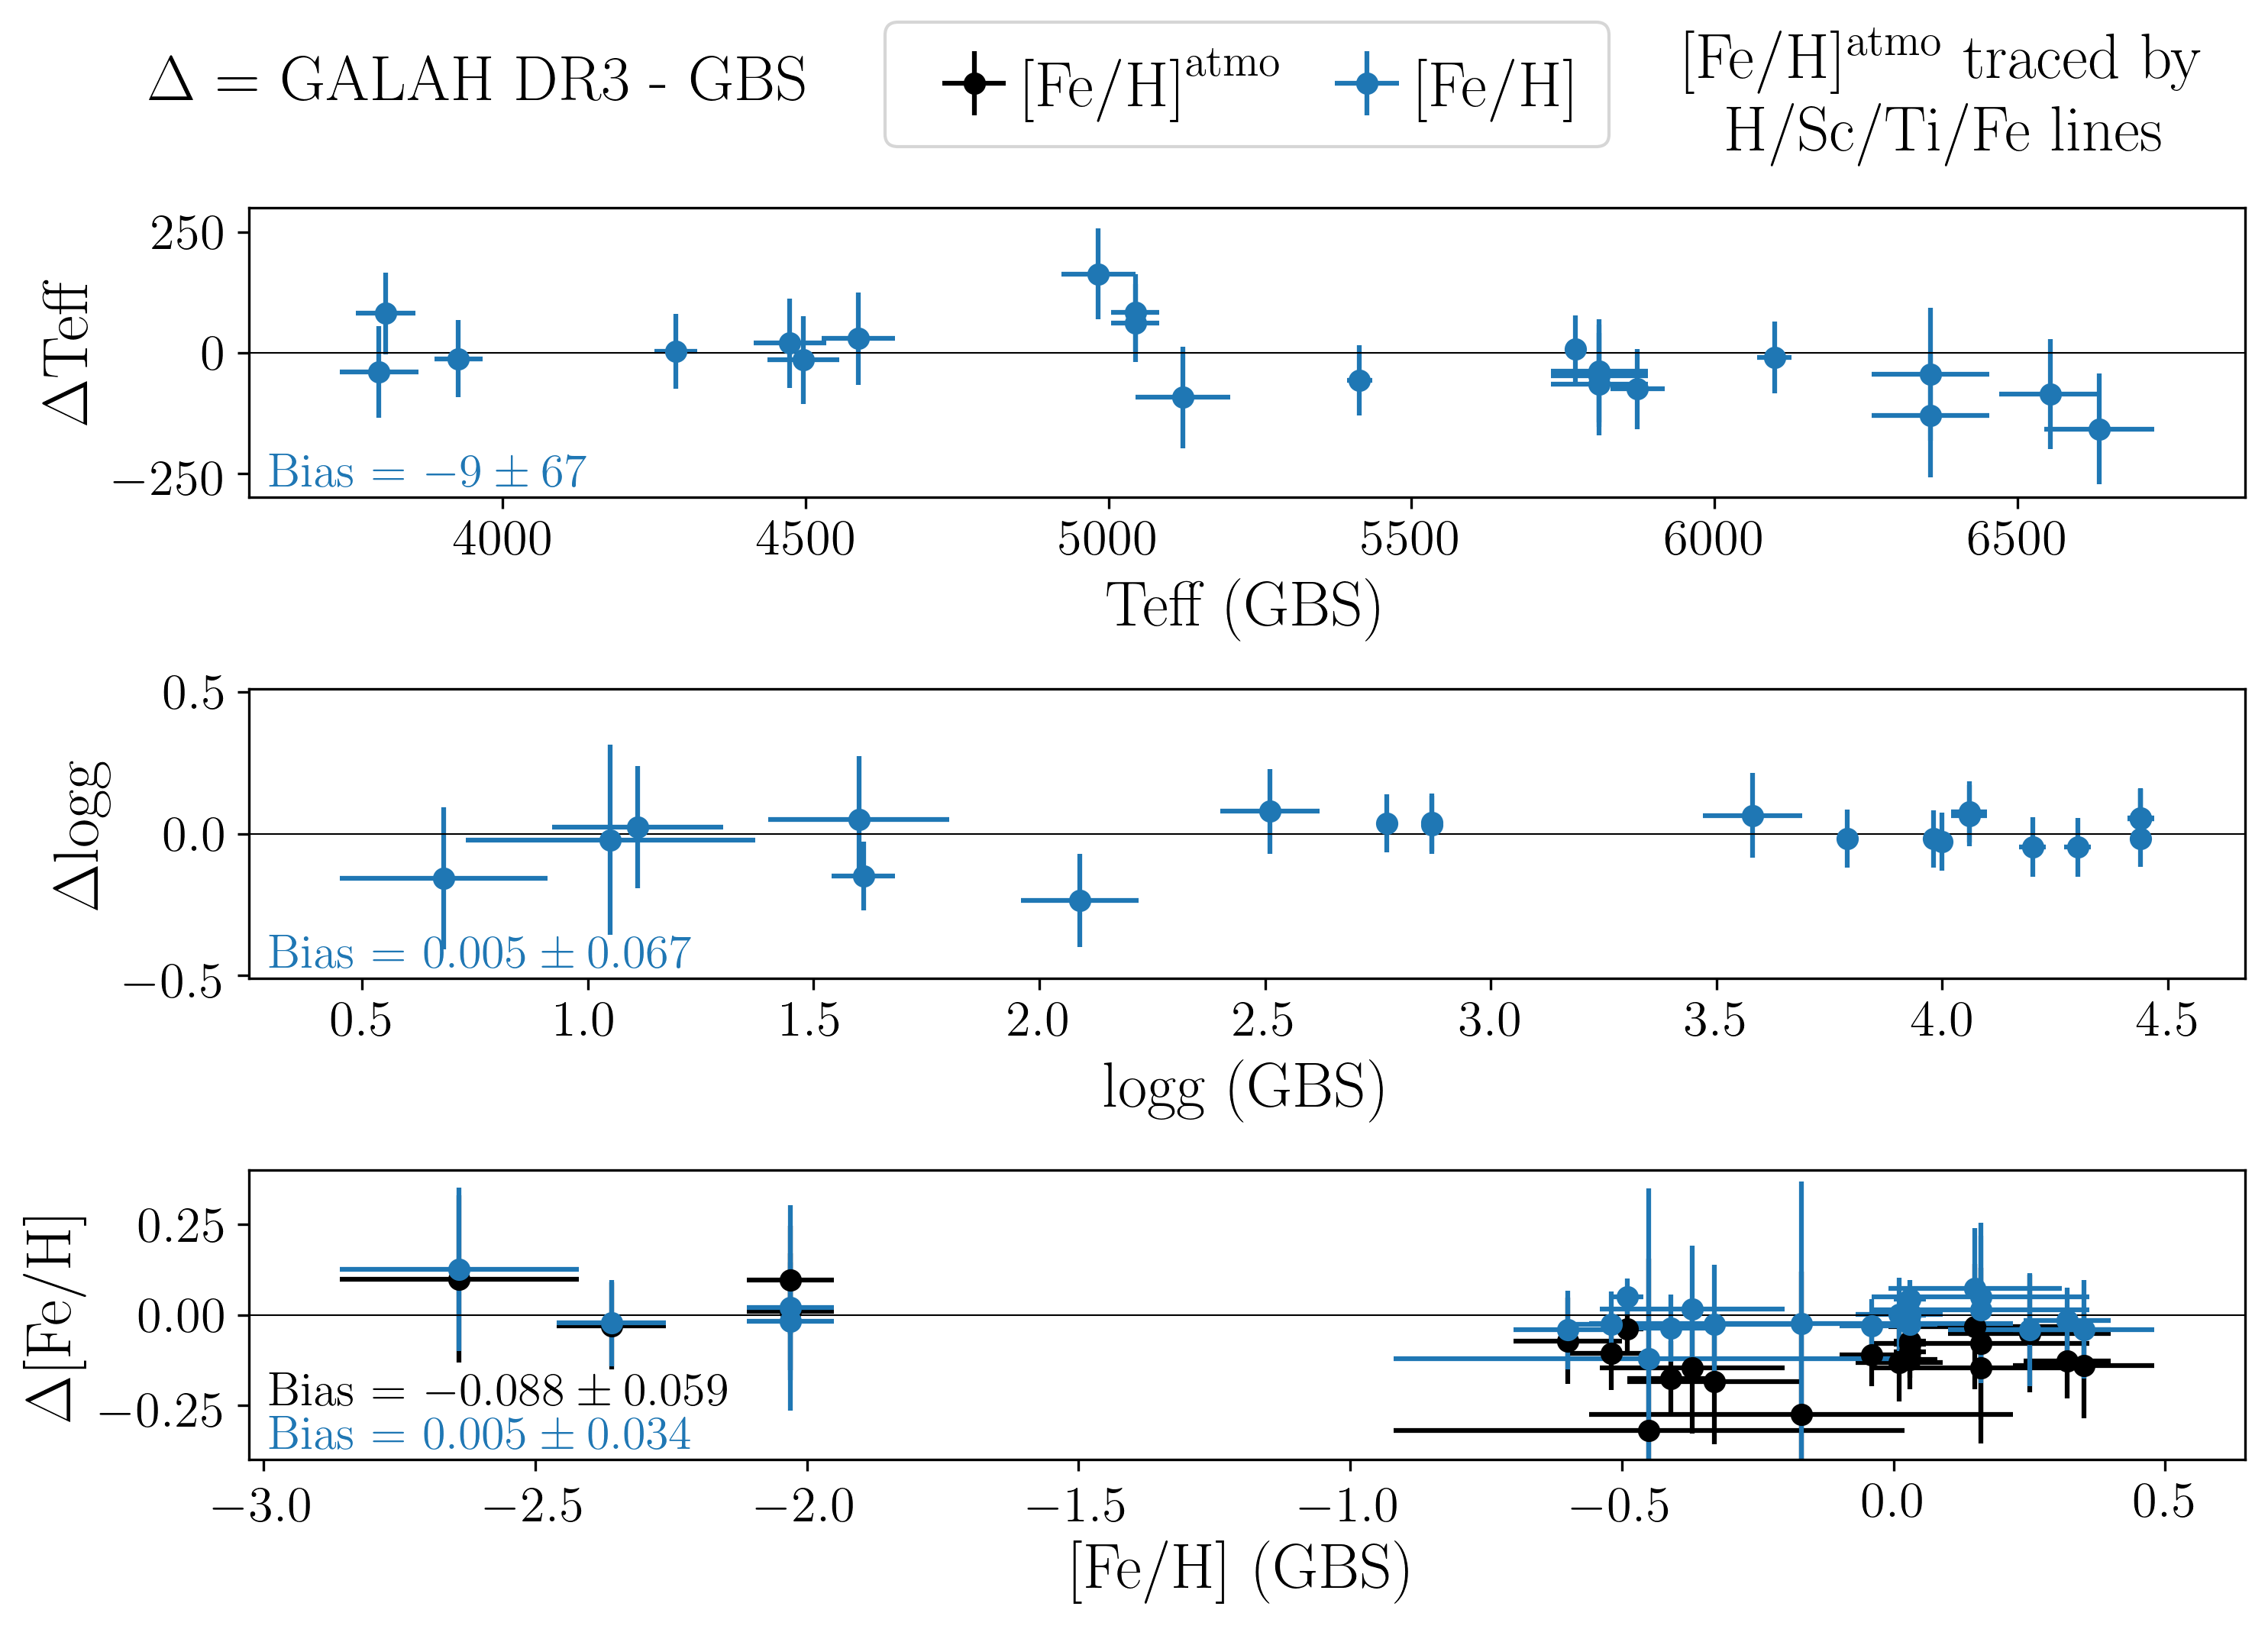
\includegraphics[width=\columnwidth]{figures/gbs_performance_lbol.png}
\caption{
\textbf{Comparison of the stellar parameters \Teff (top), \logg (middle), and \feh (bottom) for the observed Gaia FGK Benchmark stars.}
Differences are stated as GALAH DR3 - GBS \citep{Jofre2018a} and biases are error-weighted. The biases of \Teff are small but show, similar to previous data releases, systematic derivations for F stars. The biases of \logg are small thanks to the improved \logg estimation. The disagreement between the GBS $\log g$ values and ours has decreased significantly from DR2 ($-0.06\pm0.18\,\mathrm{dex}$). During the stellar parameter estimation, the atmospheric iron abundance (black error bars) is estimated from mask regions of well selected H, Ti, Sc, and Fe lines and underestimates the true iron abundance. For the abundance fits, we have thus increased the atmospheric iron abundance by $+0.1\,\mathrm{dex}$. The final reported iron abundance (blue error bars) is only based on Fe lines and shows no bias. GBS with $T_\text{eff} > 6000\,\mathrm{K}$ were observed with $S/N \sim 60$, whereas the other stars all cover $S/N$ between 150 and 800.}
\label{fig:gbs_performance}
\end{figure}

\paragraph*{IRFM temperatures}

% Based on GALAH_DR3/validation/stellar_parameters/irfm/galah_dr3_irfm.ipynb
\begin{figure*}
\centering
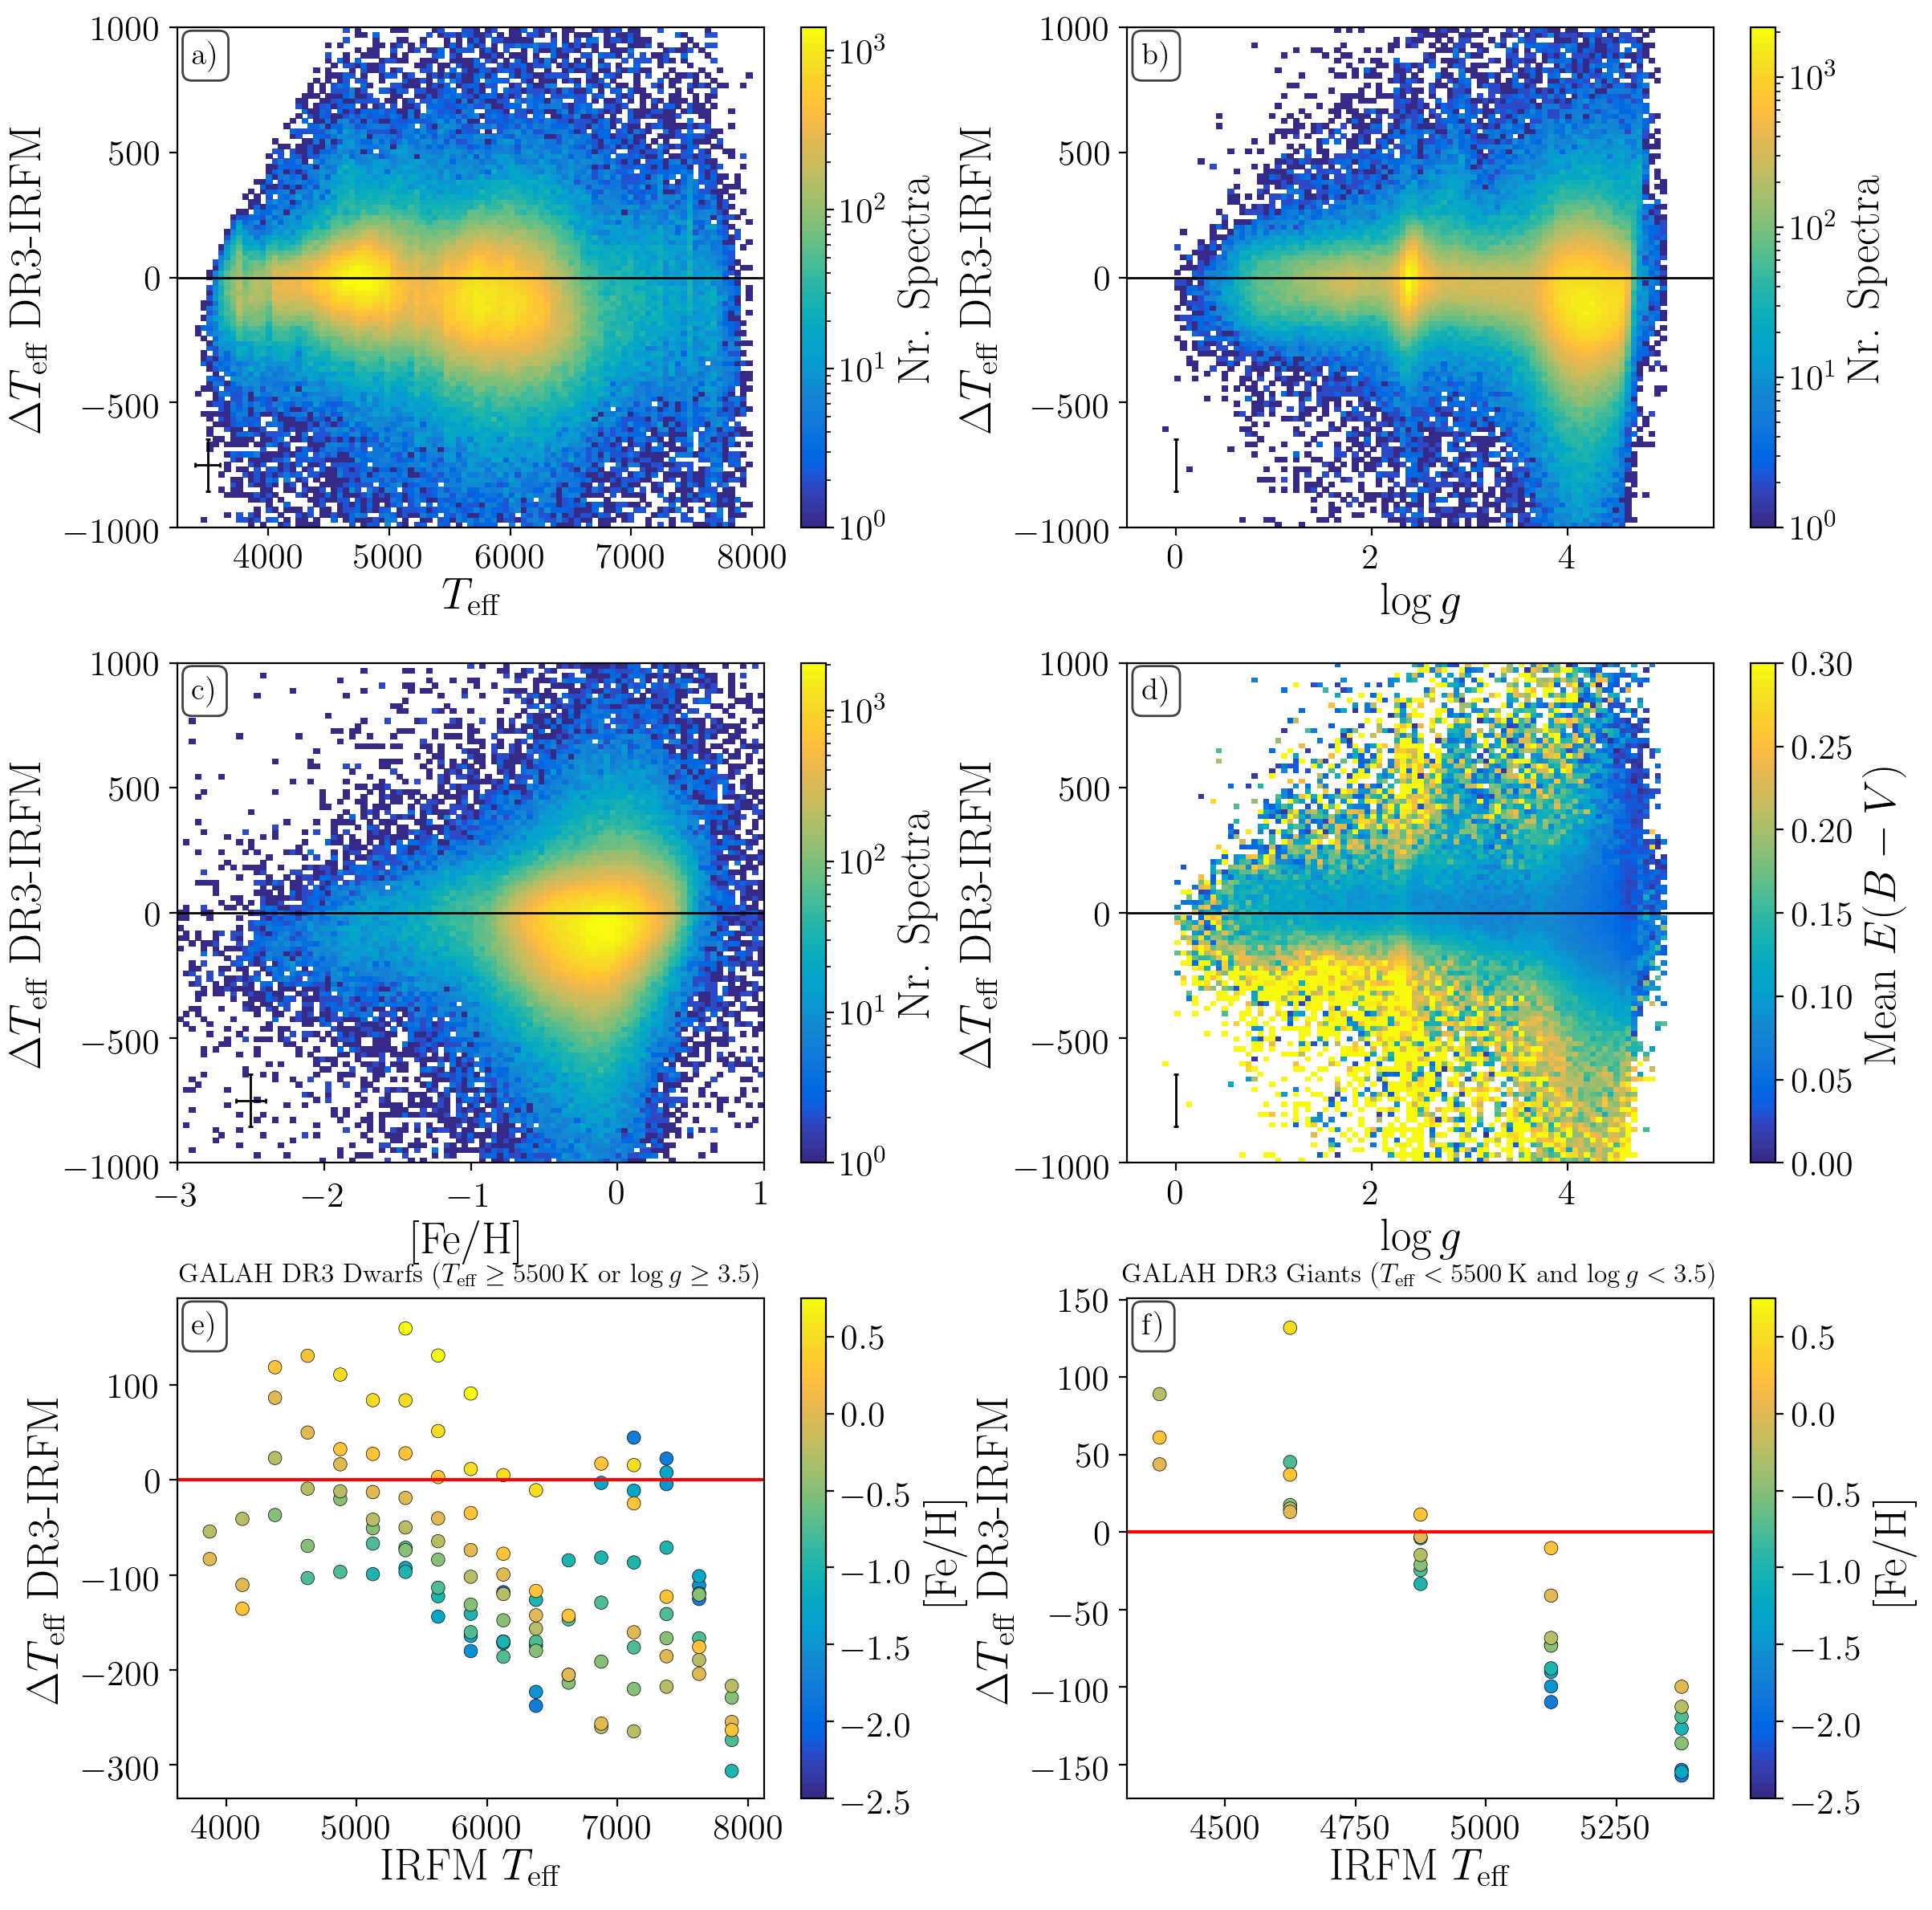
\includegraphics[width=\textwidth]{figures/plot_irfm.png}
\caption{
\textbf{Comparisons of spectroscopically determined $T_\text{eff}$ with $T_\text{eff}$ estimated via the Infrared Flux method following \citet{Casagrande2010, Casagrande2020}.} 
\textbf{Panel a-c)} Density distributions of the deviation of GALAH DR3 vs. IRFM \Teff as a function of GALAH DR3 \Teff, \logg, and \feh respectively. \textbf{Panel d)} Density distributions of the deviation of \Teff as function of GALAH DR3 \Teff colored by the mean extinction $E(B-V)$ per bin. \textbf{Panels e) and f)} Distributions of deviations of \Teff ($3875..(250)..7875\,\mathrm{K}$) as a function of IRFM \Teff for different \feh bins ($-2.50..(0.25)..0.75\,\mathrm{dex}$) for dwarfs ($T_\text{eff} \geq 5500\,\mathrm{K}$ or $\log g \geq 3.5\,\mathrm{dex}$) and giants (i.e. not dwarfs), respectively. Points are coloured by the \feh bin and represent the median deviation for bins with at least 50 stars.}
\label{fig:IRFM}
\end{figure*}

We apply the Infrared flux method \citep[IRFM][]{Casagrande2010} to estimate photometric \Teff. We use the 2MASS and \Gaia photometry to estimate photometric temperatures as described by \citet{Casagrande2020} and compare the differences between these temperatures  in Fig.~\ref{fig:IRFM}. Because the IRFM is prone to extinction, we subsequently limit the quantitative comparison (stating 16th, 50th, and 84th percentiles) to stars with small extinction $E(B-V) < 0.15\,\mathrm{mag}$ (see panel d). Most of the outliers can be explained by high extinction values (compare panel b and d).

The overall agreement is good for stars with lower temperatures ($T_\text{eff} < 5500\,\mathrm{K}$, see panel a) as well as stars with lower surface gravities ($\log g < 3.5\,\mathrm{dex}$, see panel b). We see a trend towards underestimated \Teff for hotter dwarfs, similar to previous GALAH analyses as well as the trend of the few benchmark stars.

For giants ($T_\text{eff} < 5500\,\mathrm{K}$ and $\log g < 3.5\,\mathrm{dex}$) we find a very good agreement for their whole temperature range of $-6_{-78}^{+80}\,\mathrm{K}$. For stars in the red clump region ($T_\text{eff} = 4800\pm400\,\mathrm{K}$, $\log g = 2.4\pm0.2\,\mathrm{dex}$), we find a difference of $2_{-75}^{+74}\,\mathrm{K}$.

When inspecting dwarfs ($T_\text{eff} \geq 5500\,\mathrm{K}$ or $\log g \geq 3.5\,\mathrm{dex}$) in bins of $4125..(250)..7250\,\mathrm{K}$ 
(covering $97\,\%$ of the dwarfs), we find a increasing relative trend of increasing differences from $-8_{-133}^{+138}\,\mathrm{K}$ at $4500\,\mathrm{K}$ towards $-125_{-176}^{+184}\,\mathrm{K}$ at $6750\,\mathrm{K}$. For solar twins (similar to the Solar \Teff, \logg, and \feh within $100\,\mathrm{K}$, $0.1\,\mathrm{dex}$, $0.1\,\mathrm{dex}$) we find a typical difference of $-95_{-119}^{+128}\,\mathrm{K}$.

Because the distribution of overall \Teff difference as a function of [Fe/H] (panel c) is not clear enough for a diagnostic of [Fe/H] trends, we analyse the difference as a function of different [Fe/H] bins for dwarfs (panel e) and giants (panel f).We find that our estimated \Teff best agrees for stars with solar [Fe/H] (coinciding with the peak of the GALAH MDF) but we tend to overestimate \Teff for metal-rich stars, while we tend to underestimate them for metal-poor stars.

We note that discrepancies between spectroscopic and photometric temperatures, similar to ours of $-1.3_{-2.2}^{+2.4}\,\%$ on average, are common \citep[see e.g.][]{Meszaros2013}, when not corrected. Because our spectroscopic temperatures are corresponding to the best spectroscopic fit, we decide to not correct our spectroscopic temperatures, unlike for example APOGEE \citep{Joensson2020}, but additionally we provide IRFM temperatures along with adopted reddening values in our main catalog. We note that we have not included the results of the IRFM \Teff comparisons for our accuracy estimates of our spectroscopic \Teff and therefore caution the user to decide which temperatures might be more useful for their science case and decide if they want to adjust the uncertainties by a systematic factor, for example a quadratic increase of accuracy uncertainty estimated from the difference of IRFM and spectroscopic \Teff.

\subsubsection{Surface gravity}

We see excellent agreement and negligible of biases of our derived surface gravities with those from the GBS as well as those stars with asteroseismic information. Because of the larger sample size of the stars with asteroseismic information, we apply the estimated scatter of this sample as accuracy estimate for our \logg.

\paragraph*{GBS}

The surface gravities agree very well with those of the GBS \citep{Heiter2015, Jofre2018a}, because both studies used the same approach to estimate these via bolometric relations. Due to the different implementations of this method, it is however reassuring to see the excellent agreement and low scatter (second panel of Fig.~\ref{fig:gbs_performance}). We note a slight disagreement for the highest bolometric luminosities and masses, which cancel each other out and lead to a good agreement in \logg. The only outlier of these measurements in the giant star HD~107328 (with the largest relative mass and \logg uncertainty of the GBS and a significant change from \Hipparcos to \Gaia parallaxes), for which however both \Teff and \feh are in excellent agreement with the GBS values.

\paragraph*{Stars with asteroseismic information}

We analyse a sample of 3175 spectra, for which asteroseismic \numax values are available from the K2 mission are available (Stello et al., priv. comm.), with the GALAH DR3 pipeline (`bolometric' or `lbol' pipeline) as well as with an adjusted version (`asteroseismic' or `seis' pipeline) that uses the empirical (metallicity-independent) asteroseismic scaling relations of solar-like oscillators \citep[see e.g.][]{Kjeldsen1995, Bedding2010}:
\begin{equation}
\log g = \log g_\odot + \log \frac{\nu_\mathrm{max}}{\nu_\mathrm{max,\odot}} + \log \sqrt{\frac{T_\mathrm{eff}}{T_\mathrm{eff,\odot}}}
\end{equation}
with $\nu_\mathrm{max,\odot} = 3090\,\mathrm{\upmu Hz}$ \citep{Huber2017} and $T_\mathrm{eff,\odot} = 5772\,\mathrm{K}$ (see Tab.~\ref{tab:solar_reference_values1}).

When comparing the difference of the final values for \logg estimated from the `asteroseismic' and `bolometric' pipeline (see panel a) of Fig.~\ref{fig:all_seismic}, we see a great improvement with respect to GALAH DR2 \citep[see Fig.~17 from][]{Buder2018}. Both the difference and the scatter of the \logg values has decreased down to $-0.03\pm0.12\,\mathrm{dex}$ on average and we see a good agreement with the majority of asteroseismic values (blue colorbar) for a large parameter range of $2\,\mathrm{dex}$. \SB{Dennis/Sanjib: Let me how I should update this: We note, however, several disagreements with relatively few stars. Firstly we see some outliers (green) with disagreements larger than $0.25\,\mathrm{dex}$, most notably for RC stars. These are however negligible relative to the large number of RC stars in the sample. Furthermore, we notice likely false measurements from the asteroseismic pipeline with clumps at a specific \numax value (blue) as well as false \numax values for dwarf stars (orange stars, 7.5\% of the sample). We have neglected the latter three categories when calculating the mean difference and mean trends in Fig.~\ref{fig:all_seismic}.}

\begin{figure*}
\centering
\includegraphics[width=\textwidth]{figures/logg_seis_validation_largesample.pdf}
\caption{
\textbf{Comparison of surface gravities of the stars with asteroseismic information from the K2 asteroseismic analyses (Sharma and Stello, priv. communication).}
\textbf{Panel a)} shows the density distribution of the deviation between our surface gravities (lbol) and those estimated from scaling relations (seis). Orange points indicate spectra with unreliable asteroseismic values because of detection limits of $\nu_\text{max}$ values due to the cadence of the K2 observations.
\textbf{Panel b)} showing the same stars, but in the Kiel diagram, illustrating that the detection limits of the asteroseismology causes an overdensity around $\log g \sim 3\,\mathrm{dex}$ and typically underestimated $\nu_\text{max}$ for higher $\log g$.
}
\label{fig:all_seismic}
\end{figure*}

Additionally, we have used the pipeline where \logg is a free parameter for the spectrum fit (`bolometric') to assess the improvement of our parameter estimation thanks to the use of external information, see Fig.~\ref{fig:seis_comparison_3setups}. The free pipeline can only estimate \logg from the spectra and shows a significant scatter (especially for the red clump stars) for this stellar parameter, which propagates into larger scatters for \Teff and \feh as well. With the new constraints on \logg from external information from astrometry and photometry, the scatter of all parameters decreases significantly and the red clump stars show a tight distribution around $\log g \sim 2.4\,\mathrm{dex}$, consistent with the most reliable measurements, which take into account asteroseismic information (right panels).

\begin{figure*}
\centering
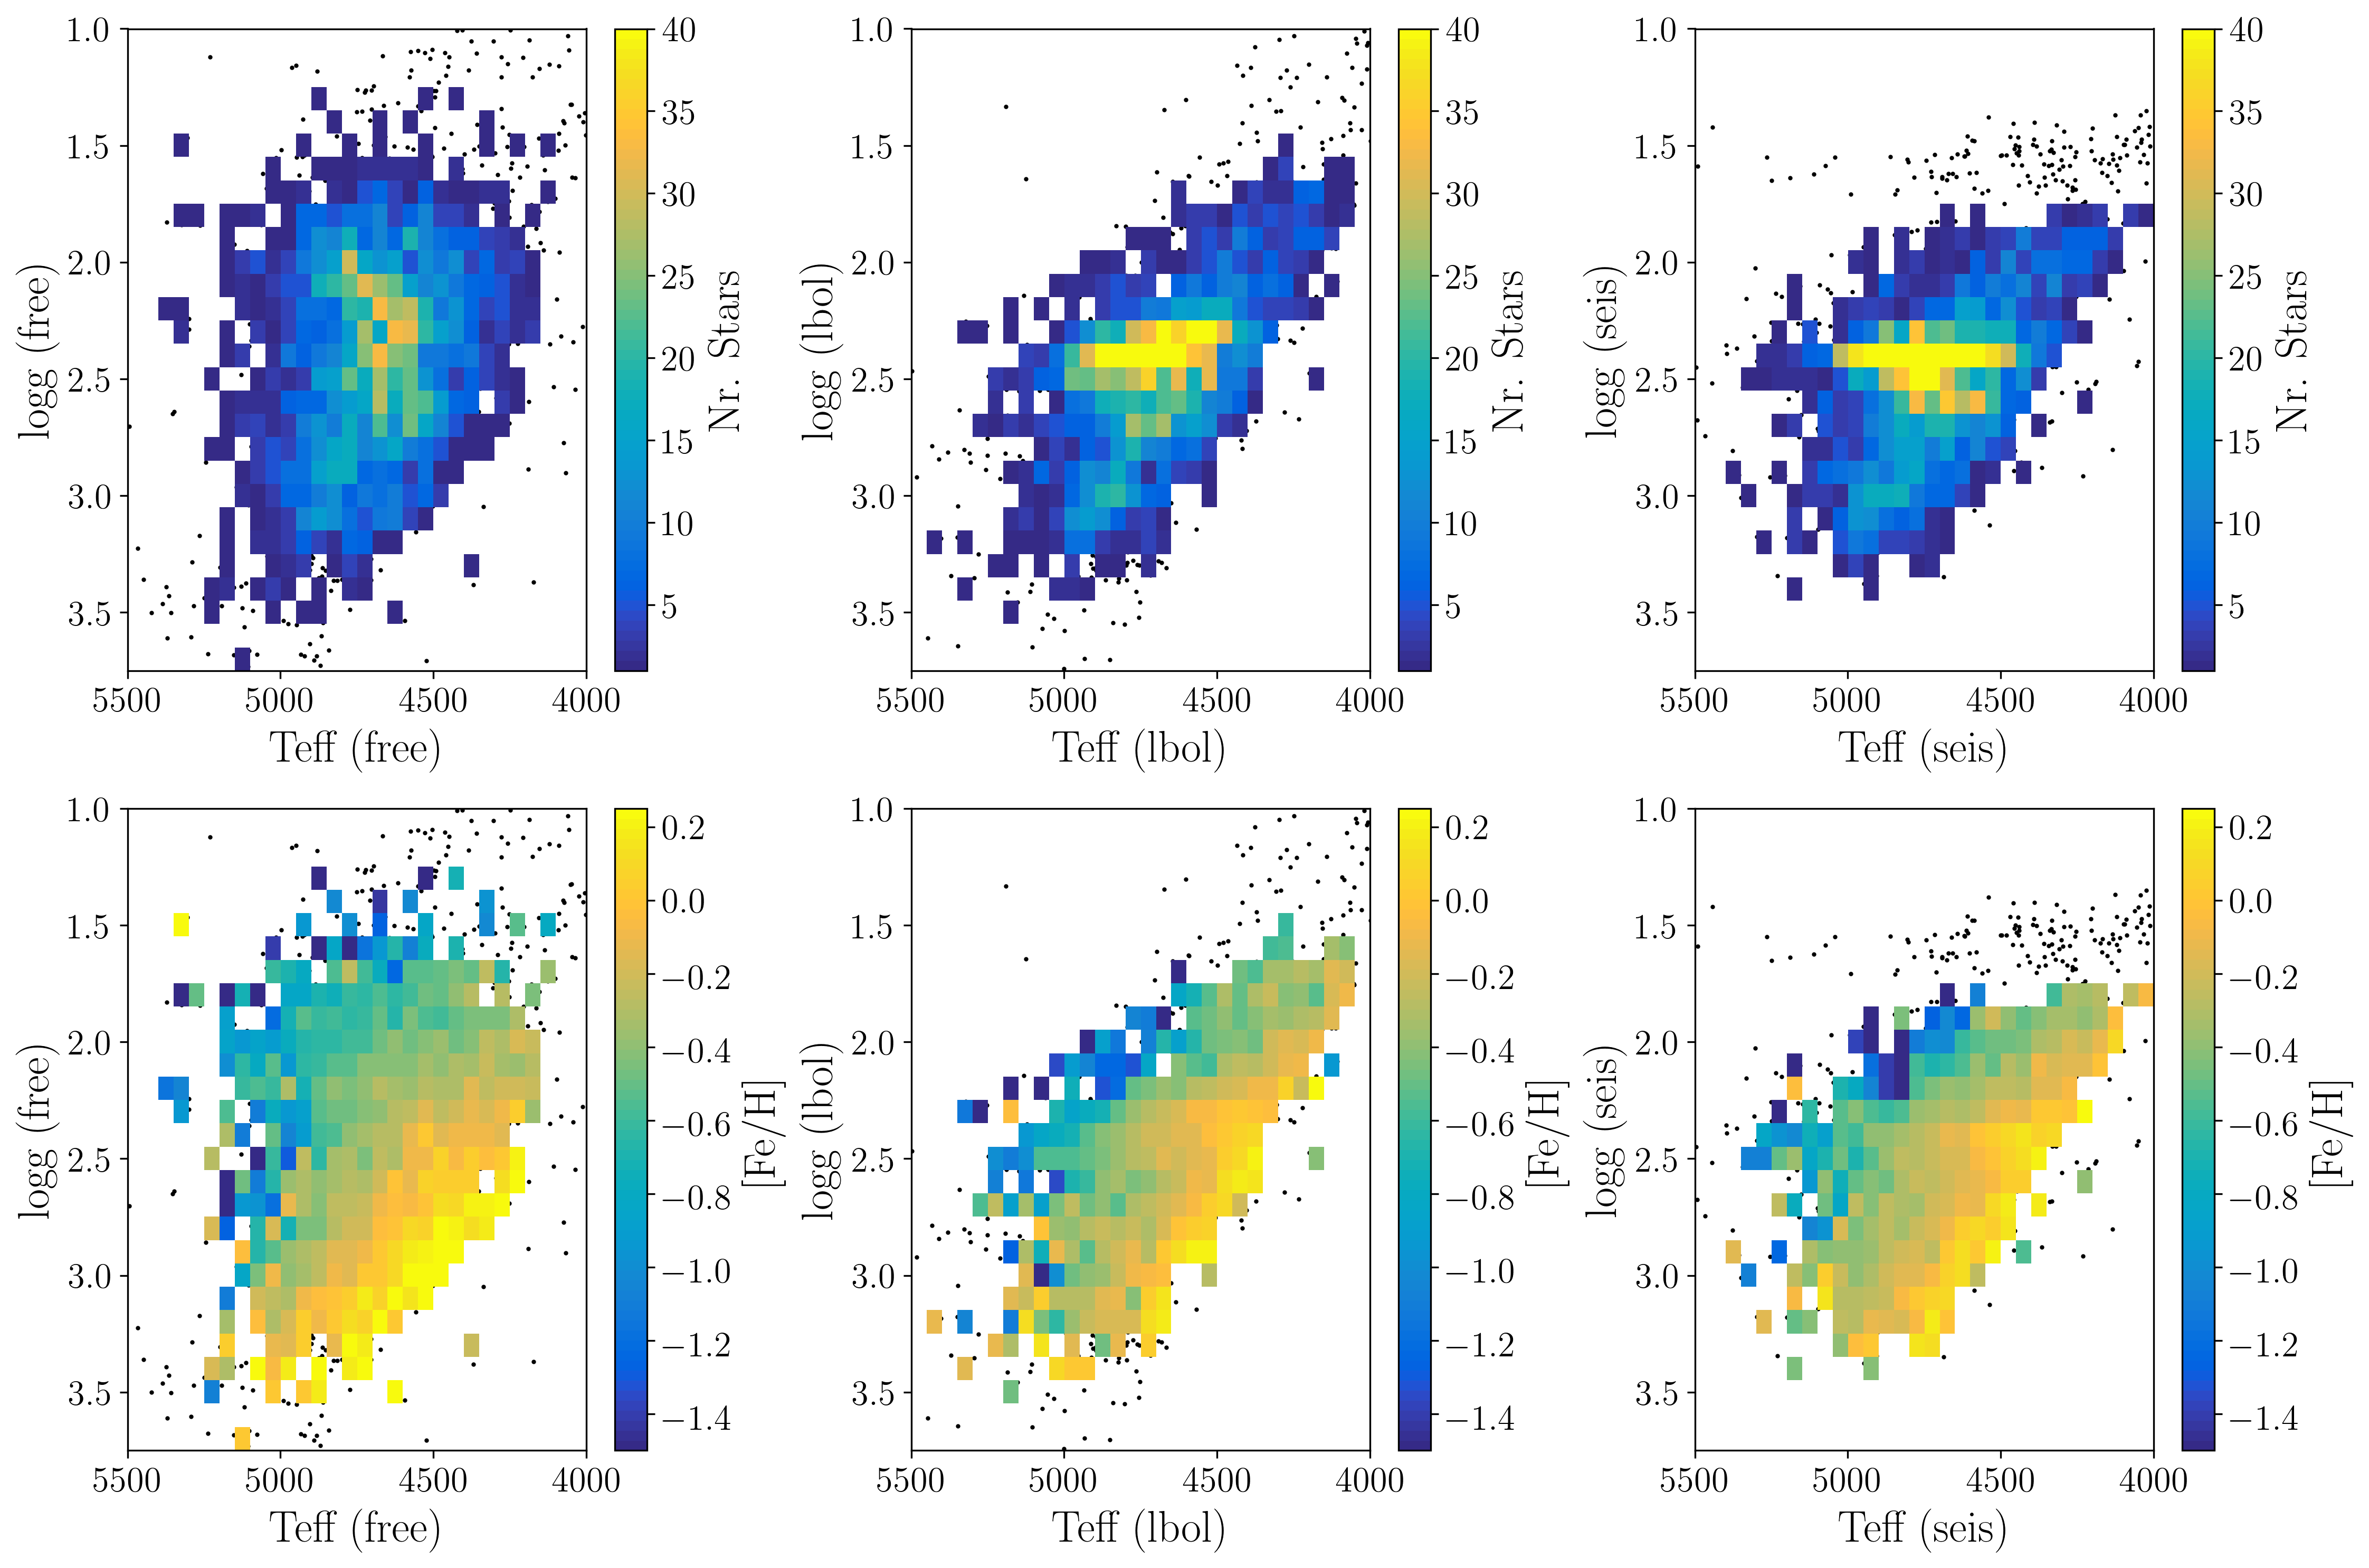
\includegraphics[width=\textwidth]{figures/seis_comparison_3setups.png}
\caption{
\textbf{Performance of GALAH synthesis pipeline in with the `free' (left panels), `bolometric' (middle panels), and `seismic' (right panels) pipeline for the stars for asteroseismic and parallax information.}
Shown are the number density (upper panels) as well as the mean iron abundance (lower panels) in binned distributions.
}
\label{fig:seis_comparison_3setups}
\end{figure*}

\subsubsection{Metallicity and iron abundance}

For GALAH DR3, we use different notations of the commonly used values for metallicity [M/H] and iron abundance [Fe/H]. We strictly seperate those and also refer to the atmosphere iron abundance \textsc{fe\_h\_atmo} (of the {\sc marcs} grids and {\sc sme}.feh). The latter is estimated mainly from Fe lines, but we also included Sc and Ti lines and thus would refer to it as pseudo-iron abundance. Only when we talk about the abundance estimated from Fe lines, we refer to [Fe/H] or \textsc{fe\_h}. We report the scatter of our measurements with those of the GBS as accuracy measures for both atmosphere (\textsc{fe\_h\_atmo}) and pure iron abundance \textsc{fe\_h}.

\paragraph*{GBS}

After the collection of results from the stellar parameter estimations, we compare the atmosphere iron abundance with the values from \citet{Jofre2018a} and find a significant bias (see black errors bars in bottom panel of Fig.~\ref{fig:gbs_performance}). We have thus decided to shift the atmosphere value \textsc{sme}.feh by $+0.1\,\mathrm{dex}$ for the later abundance estimations.

From the observation of the sky flat, we estimate a final zeropoint value of $A(\mathrm{Fe})_\odot = 7.38$. This value is significantly smaller than the literature values of 7.45 and 7.50 from \citet{Grevesse2007} and \citet{Asplund2009}, respectively, and points towards confirms that the absolute iron abundances would be estimated too low without zeropoint shifts. When using this value for the computation of the final [Fe/H] values however, we find not only the Solar values, but also the GBS stars to be in agreement with the literature. We furthermore see that the scatter of this pure [Fe/H] value is smaller than of the atmosphere values (compare black and blue in panel c) of Fig.~\ref{fig:gbs_performance}).

We note, however, that the coverage of the GBS in terms of iron abundance is very sparse. This is easily visible in the bottom panel of Fig.~\ref{fig:gbs_performance} for the iron abundances around $-1.5\,\mathrm{dex}$, but also concerns the most metal-rich stars, especially giants, for which we have to assume that the general agreement also applies.

\subsubsection{Radial velocities}

Contrary to GALAH~DR2, we have estimated the radial velocities as a free parameter in the stellar parameter estimation and have thus been able to overcome a systematic trend of the reduction pipeline, overestimating the absolute radial velocity by $1\%$.

When comparing our radial velocities with those by \Gaia DR2, see Fig.~\ref{fig:radial_velocities}, we find that the difference between the estimated radial velocities (see panel a) for the unflagged stars with $S/N > 40$ can be best fitted with two Gaussian distributions, one narrow Gaussian with a means of $0.21\,\mathrm{km/s}$ and standard deviation of $0.52\,\mathrm{km/s}$ and one broader Gaussian with $0.10\,\mathrm{km/s}$ and a standard deviation of $1.54\,\mathrm{km/s}$. These fits already exclude most of the stars with significant differences between the GALAH and \Gaia observations (see panel b), which are in most cases caused by binarity or other spectroscopic variablities. Except for the bias, which points in the same direction as the bias of $0.32\,\mathrm{km/s}$ estimated for RAVE~DR6 \citep{Steinmetz2020a}, we find no large systematic trend between GALAH and \Gaia radial velocities.

As for GALAH DR2, we have estimated an accuracy of $0.1\,\mathrm{km/s}$ for the reported radial velocities as part of this pipeline, but also report a more accurate estimate with the approach by \citet{Zwitter2018}.

% Made with GALAH_DR3/validation/stellar_parameters/gaia_dr2_radial_velocities/radial_velocity_comparison_gaia_dr2.ipynb
\begin{figure*}
\centering
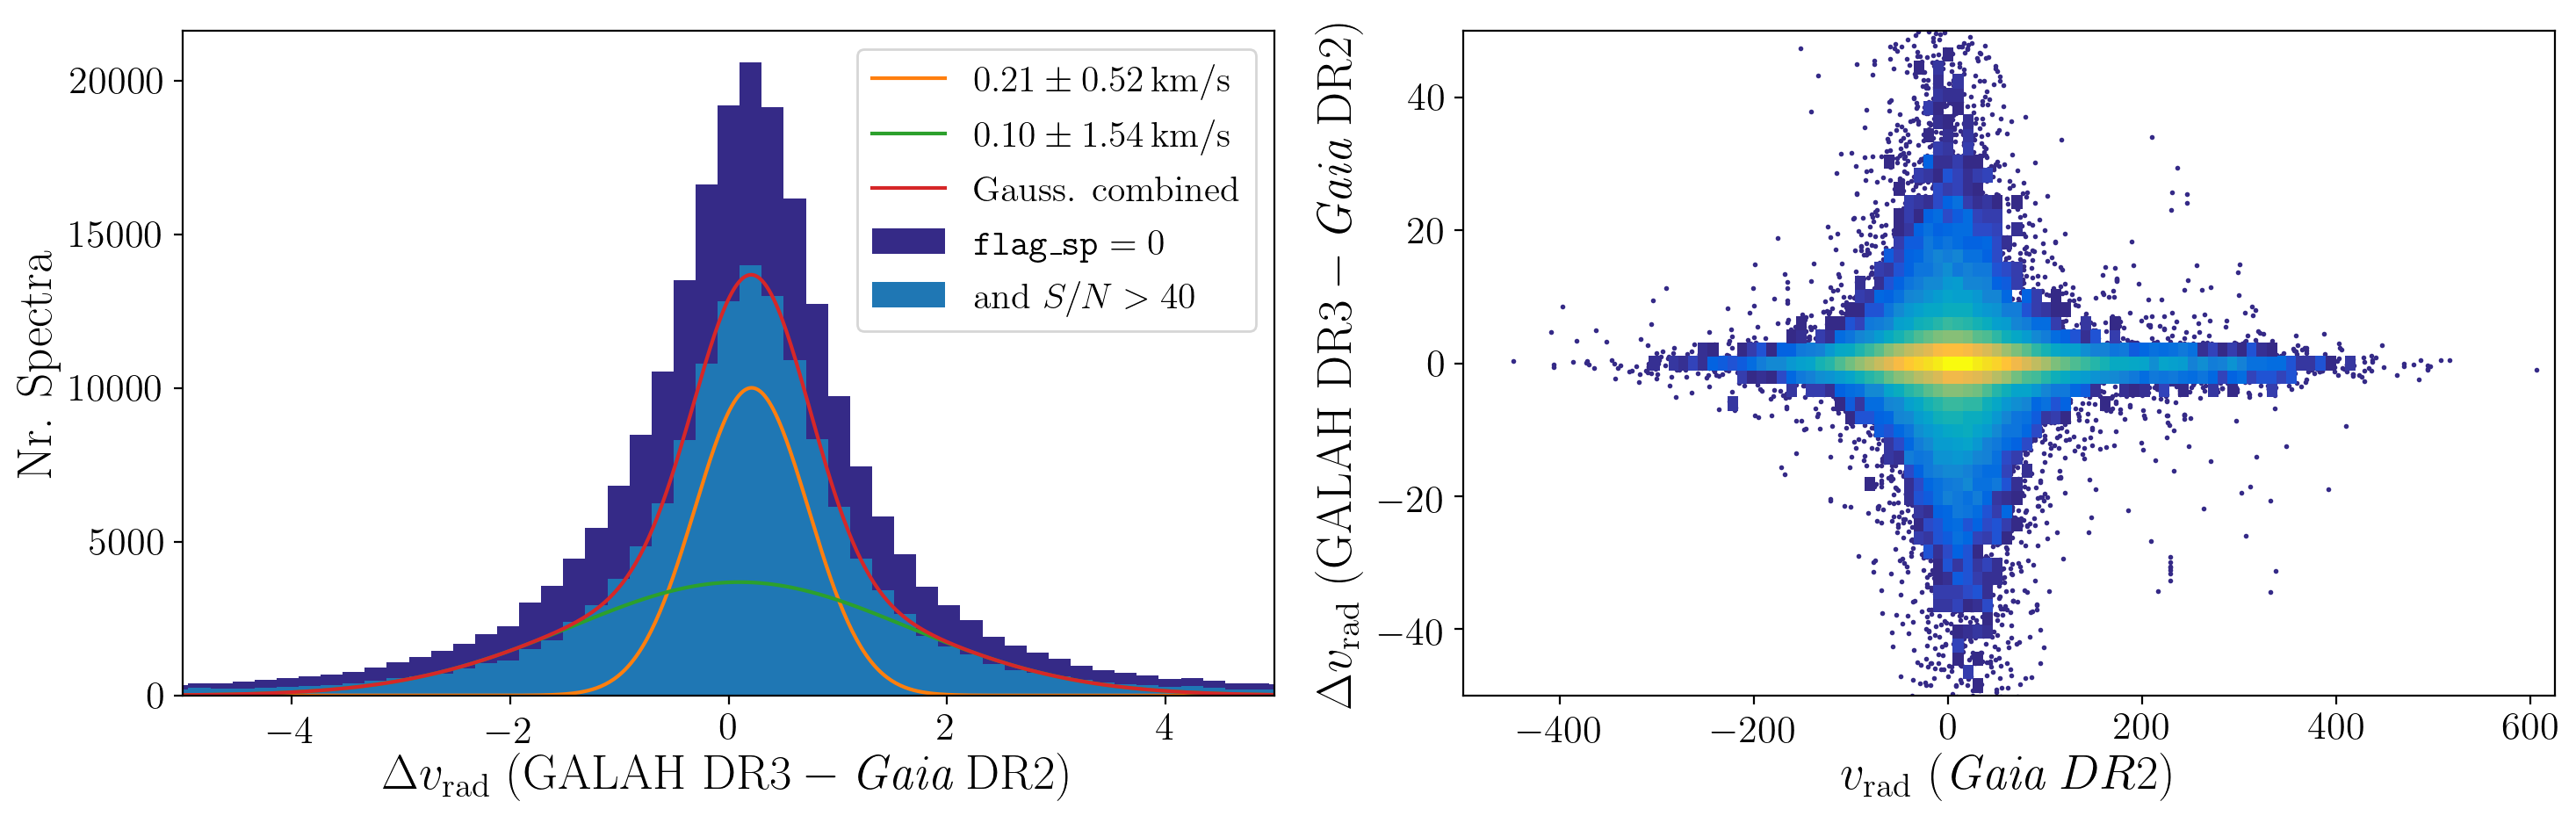
\includegraphics[width=\textwidth]{figures/radial_velocity_comparison.png}
\caption{Comparison of radial velocities from GALAH DR3 (this work) with \Gaia DR2. Left panel: Differences between the estimated radial velocities for stars with $\texttt{flag\_sp}=0$ and all $S/N$ (dark blue) and only above $\texttt{snr\_c2\_iraf} > 40$. Similar to the RAVE collaboration \citep{Steinmetz2020a}, two Gaussian curves fit the distribution significantly better.}
\label{fig:radial_velocities}
\end{figure*}

\subsection{Precision of stellar parameters} \label{sec:precision_sp}

To estimate the precision of stellar parameters, we use both internal {\sc sme} covariance errors and repeated observations of the same star for all stellar parameters except for \logg, for which we Monte Carlo sample the uncertainties.

\SB{Future: Estimate repeat observation as a function not only of SNR, but also Teff and [Fe/H], similar to APOGEE DR16 (Joensson et al. 2020)}

\subsubsection{\Teff, \feh, \fehatmo, \vbroad, \vrad}

We have estimated the standard deviations of repeated observations for the same fiber, different fibers, and irrespective of the fibre and plot their standard deviations as a function of $S/N$ in CCD2\footnote{For the repeat observations we us the $S/N$ of the higher quality observation.} together with the median {\sc sme} covariance errors in Fig.~\ref{fig:precision_sp} for the fitted stellar parameters $T_\text{eff}$, $\log g$, iron line abundance [Fe/H], the atmosphere iron abundance [Fe/H], rotational broadening $v_\text{broad}$, and radial velocity $r_\text{rad}$. 

% Made with GALAH_DR3/validation/repeat_observations/estimate_repeat_uncertainty.ipynb
\begin{figure*}
\centering
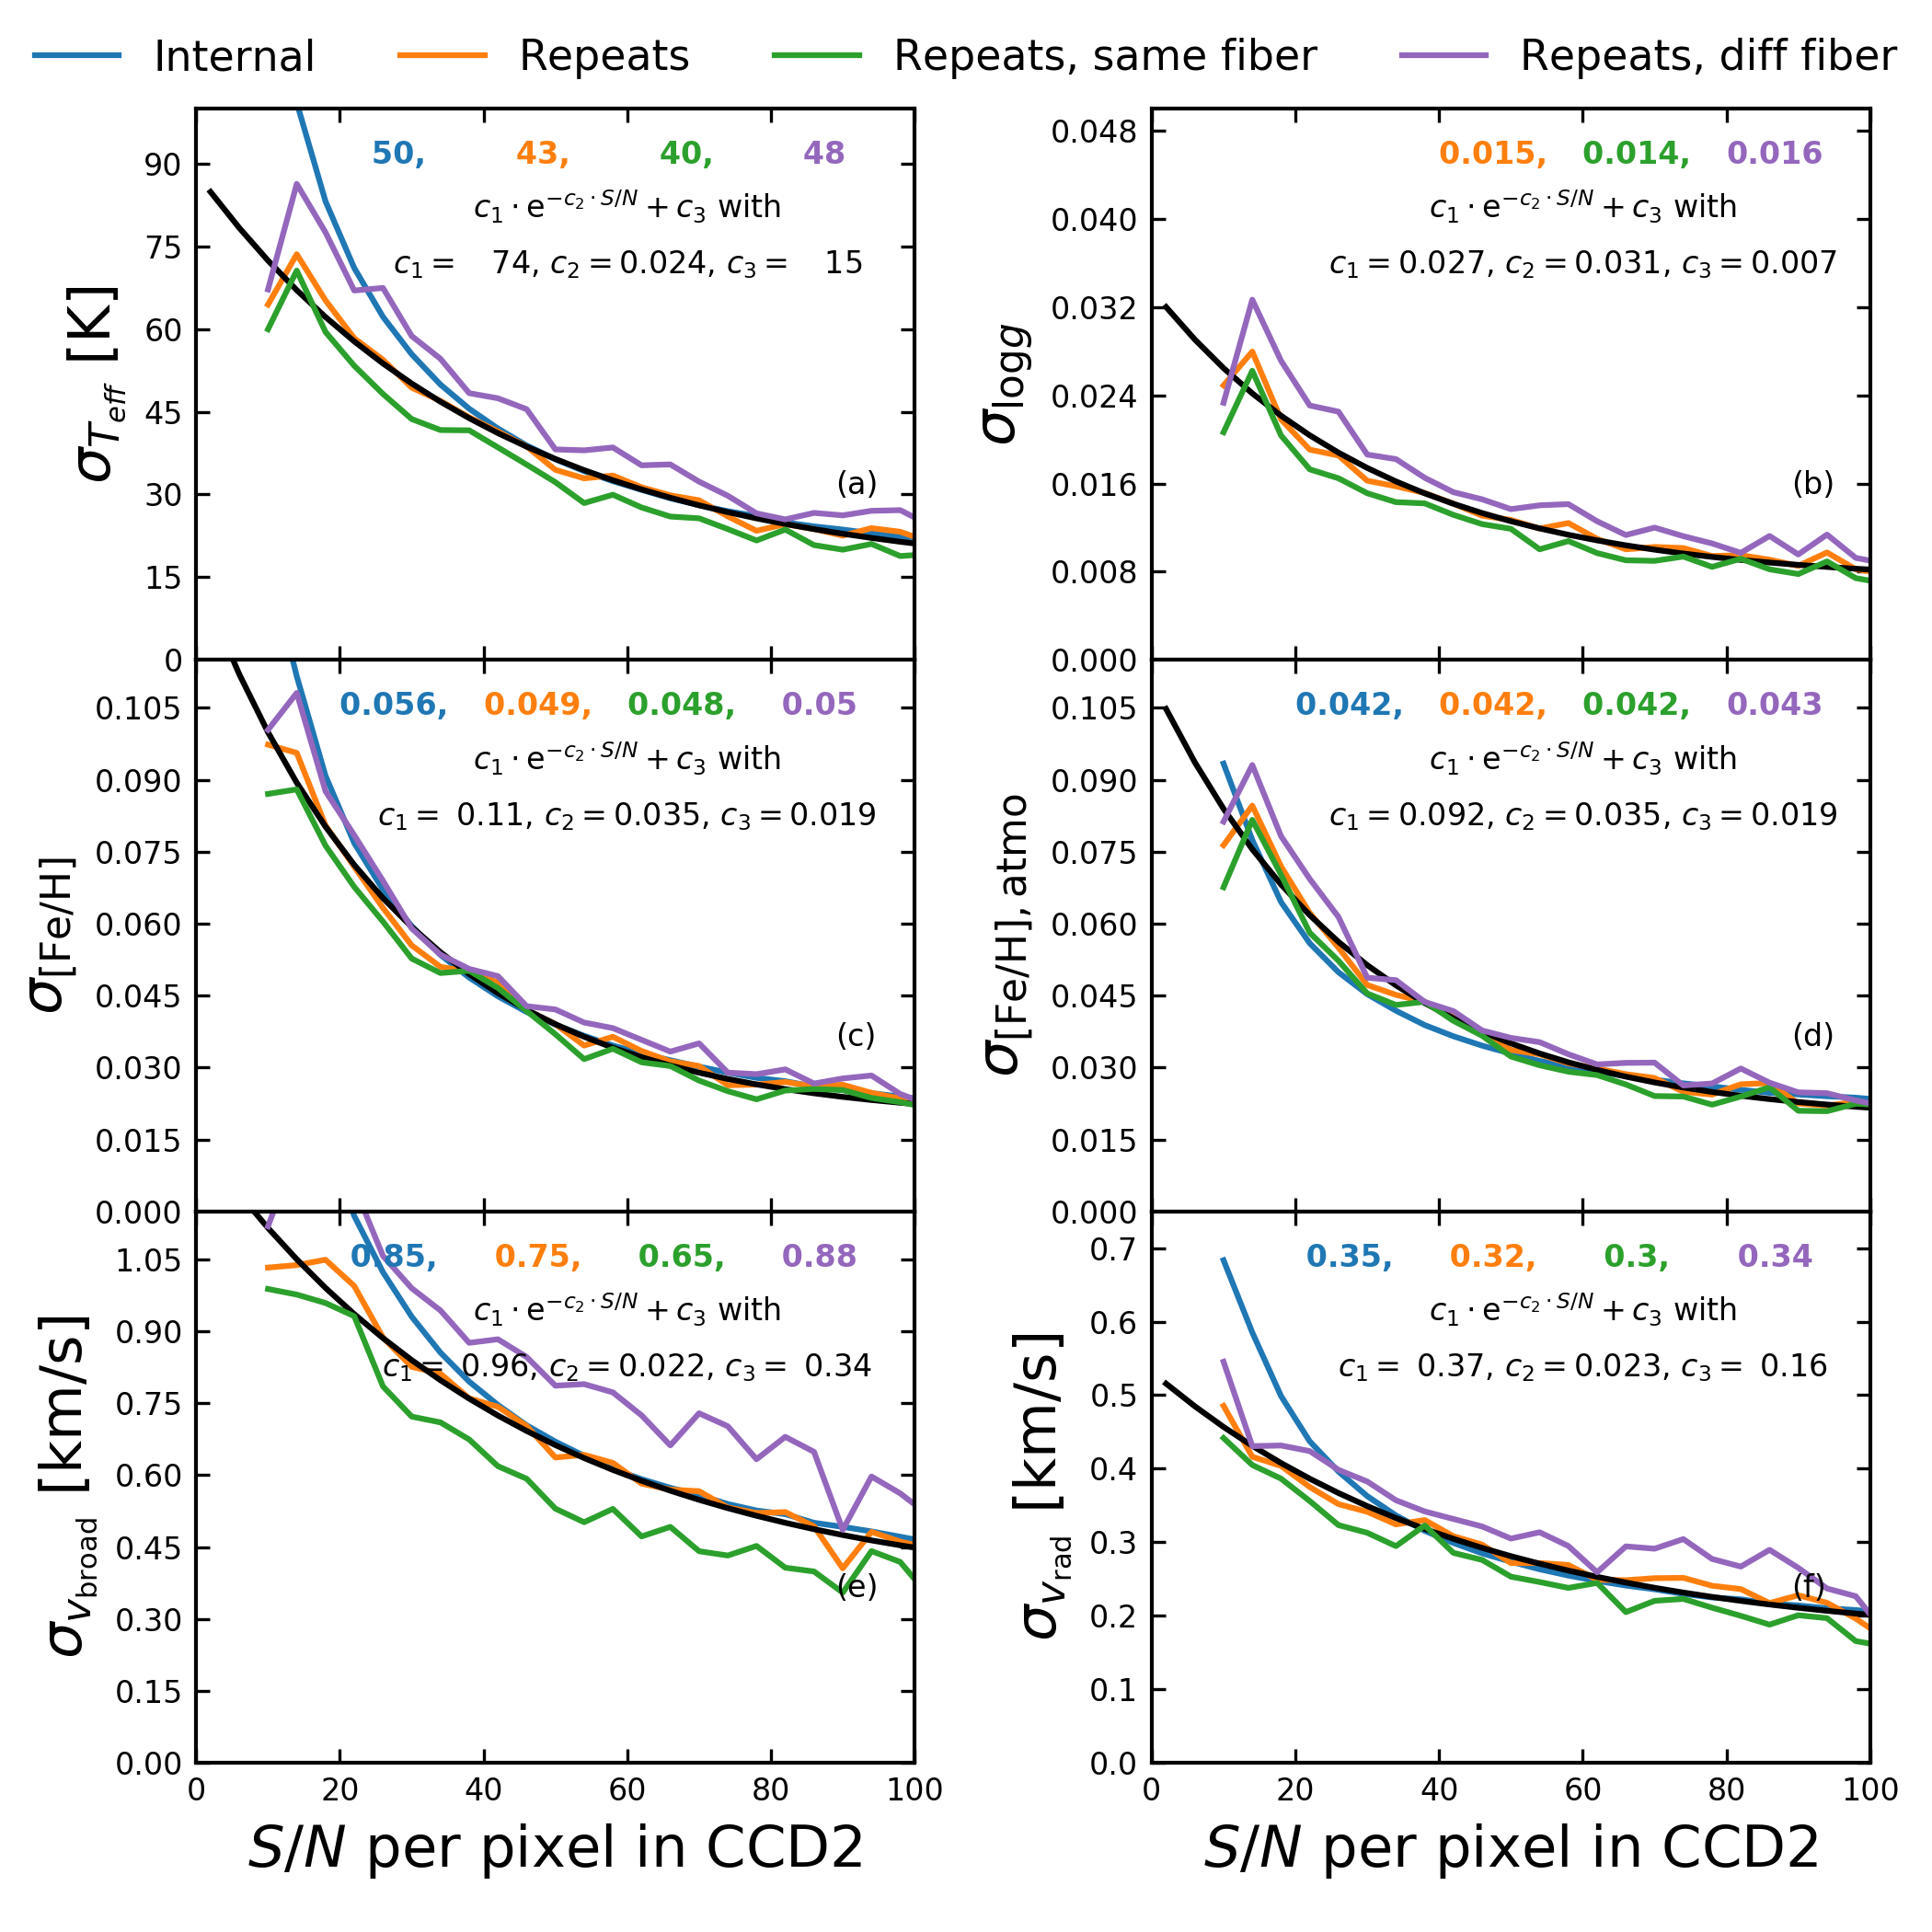
\includegraphics[width=\textwidth]{figures/repeat_uncertainties_snr_flag0.png}
\caption[{Precision estimates for stellar parameters.}]{Precision estimates from internal {\sc sme} covariance uncertainties (blue) as well as standard deviations from all (orange), same fibre (green), and different fibre (violet) repeat observations. The numbers in each panel indicate the uncertainties estimated for $S/N = 40$ per pixel, similar Fig. 15 from \citet{Buder2018}. Note that the internal precision was already adjusted for each parameter with the scaling relations outlined in the text.}
\label{fig:precision_sp}
\end{figure*}

The trends of internal and repeat precision are expected to be similar, but we find that, for the stellar parameters, the uncertainties from the internal {\sc sme} covariance uncertainties are typically significantly lower than those from repeat observations. As discussed when introducing the final error estimation with Eq.~\ref{eq:final_error}, the two precision estimates should be the same and we thus rescale the internal {\sc sme}-based uncertainties with a combination of slopes and shifts, noted as (slope,shift) with (3,7.5) for \Teff,(4,0.01) for \feh, (2,0.0125) for \fehatmo, (1.75,0.3) for \vbroad, and (2.0,0.15) for \vrad towards a minimum difference and slope with respect to the exponential fit for the repeat observations (black curve in Fig.~\ref{fig:precision_sp}). For the estimation of these linear rescaling functions, we have focused on the $S/N$ interval of 40 to 200, which typically leads to larger internal uncertainties for those stars below $S/N < 20$, for which we believe a more conservative uncertainty estimate is justifiable.

These rescaled internal precision allow now a combination of the individual estimate of the fit quality (through the internal {\sc sme}-based uncertainty) with the general precision expected for a given $S/N$, which could otherwise be underestimated when only using to the raw internal uncertainty. 

We further note that we have changed our definition of $S/N$ in these figures to show the $S/N$ of the higher quality observation. The quantitative increase of the precision from GALAH DR2 to GALAH DR3 is thus not an indicator of the decreasing precision, but that we estimate the precision more reliably.

\paragraph*{Precision of surface gravities \logg}

We stress that $\log g$ values are not optimised from the $\chi^2$-determination of the spectra like the other parameters, but from Eq.~\ref{eq:logg}. Instead of the internal {\sc sme} uncertainties, we sample the parameters used for Eq.~\ref{eq:logg} via MC sampling. For computational reasons, we assume the uncertainties for the formula to be Gaussian and sample the parameters with uncertainties $\sigma (M) = 0.1\cdot M$, $\sigma (BC) = 0.1\,\mathrm{mag}$, $\sigma (T_\text{eff})$, $\sigma (D_\varpi)$, $\sigma (K_s)$, and $\sigma (A_{K_s})$. With this approach we estimate a mean internal uncertainty for \logg of $0.07\,\mathrm{dex}$.

By construction and due to the exquisite astrometric and photometric external information available, this internal precision is significantly better than the previous spectroscopic estimates from GALAH DR2. We note however, that these estimates do not take external influences like binarity or correlations of uncertainties into account.

\paragraph*{Iron abundances of cluster stars}

When using the open cluster membership analysis by \citet{CantatGaudin2020}, we estimate that we have intentionally and unintentionally observed members of 75 stellar clusters. The eight open clusters with most observations are NGC~2682 (278 spectra, M~67), NGC~2632 (117, M44, Praesepe), NGC~2516 (83), NGC~2204 (81), Ruprecht~147 (80), Melotte~22 (74), Blanco~1 (67), and NGC~6253 (50). Furthermore we have observed 10 of the 128 open clusters\footnote{These are ASCC~16 (22 spectra), ASCC~16 (22), ASCC~21 (11), Berkeley~33 (8), Melotte~22 (74), NGC~2204 (81), NGC~2232 (20), NGC~2243 (8), NGC~2318 (2), NGC~2682 (278), and Ruprecht~147 (80).} of the OCCAM survey \citep{Donor2020}, included as VAC from SDSS DR16 \citep{SDSSDR16}. Because the analysis of all open clusters observed with GALAH will be addressed in the dedicated paper by \SB{LASTNAME, F. et al (in prep.) - Who is working on that? Gayandhi, Lorenzo, Chen?}, we only focus on these eight open clusters which cover a large range of evolutionary stages and additionally compare the four clusters of them which are also reported by the OCCAM survey.

We show the coverage of evolutionary stages for these clusters in the first and fourth panel of Fig.~\ref{fig:oc_stellar_params} to illustrative the coverage of these cluster by GALAH as well as OCCAM (the latter cover typically showing a significantly larger amount of observations if available). When looking at the average values of [Fe/H] for these clusters as a function of \Teff (2nd and 5th panels) as well as \logg (3rd and 6th panels), we firstly see very good agreement for the average values of NGC~2682, NGC~2204, and Melotte~22 between GALAH and OCCAM, and only a disagreement for Ruprecht~147 with a lower [Fe/H] estimated with a simple average by GALAH. \SB{Should we calculate a more robust mean?} \LS{The purpose of this section is to check our results and compare them to those from OCCAM, so I think that the way that you have done so far is very simple (which is a virtue) and clear. Maybe, if you really want to change something, I think that the median would be better than the mean and then use the standard error of the mean.} We have limited the stars used for this averaging to stars with $4500 < T_\mathrm{eff} < 6500\,\mathrm{K}$. We limit this cut on the hot side, because we see significant trends for stars with temperatures above this cut, for example for NGC~2516. On the cool side we see a significant trend of decreasing [Fe/H] cool stars for NGC~2204 (for GALAH) and Ruprecht~147 (for OCCAM). \SB{Check in Donor+2020, why OCCAM also reports these significantly low values of [Fe/H] for cool giants in Ruprecht 147. We should at least discuss this here. But in general we see good agreement! Should we check individual spectra/stars? When I did that via TOPCAT for those 4 clusters, the agreement was quite good.}

\SB{We should write something about the globular clusters as well!}

\DN{Use some of the 8 GCs covering the lower [Fe/H] range. Fig.~\ref{fig:gc_feh}. Overplot isochrones?, e.g. \citep{Thygesen2014} 12Gyr [Fe/H]=-0.73, [alpha/Fe] = 0.33}

We also overplot APOGEE~DR16 which are likely members of 47~Tuc\footnote{We selected these stars within certain deviations from the mean cluster estimates reported by \citet{Baumgardt2019}, i.e. $\alpha = 6.02 \pm 3\,\mathrm{deg}$,  $\delta = 72.08 \pm 3\,\mathrm{deg}$, $v_\text{rad} = -17.45 \pm 15 \,\mathrm{km/s}$, $\mu_\alpha = 5.25 \pm 1.5\,\mathrm{mas/yr}$, and $\mu_\delta = -2.53 \pm 1.5\,\mathrm{mas/yr}$ from APOGEE DR16}.

% Created with GALAH_DR3/validation/comparisons/comparison_clusters/GALAH_DR3_Comparison_Clusters.ipynb
\begin{figure*}
\centering
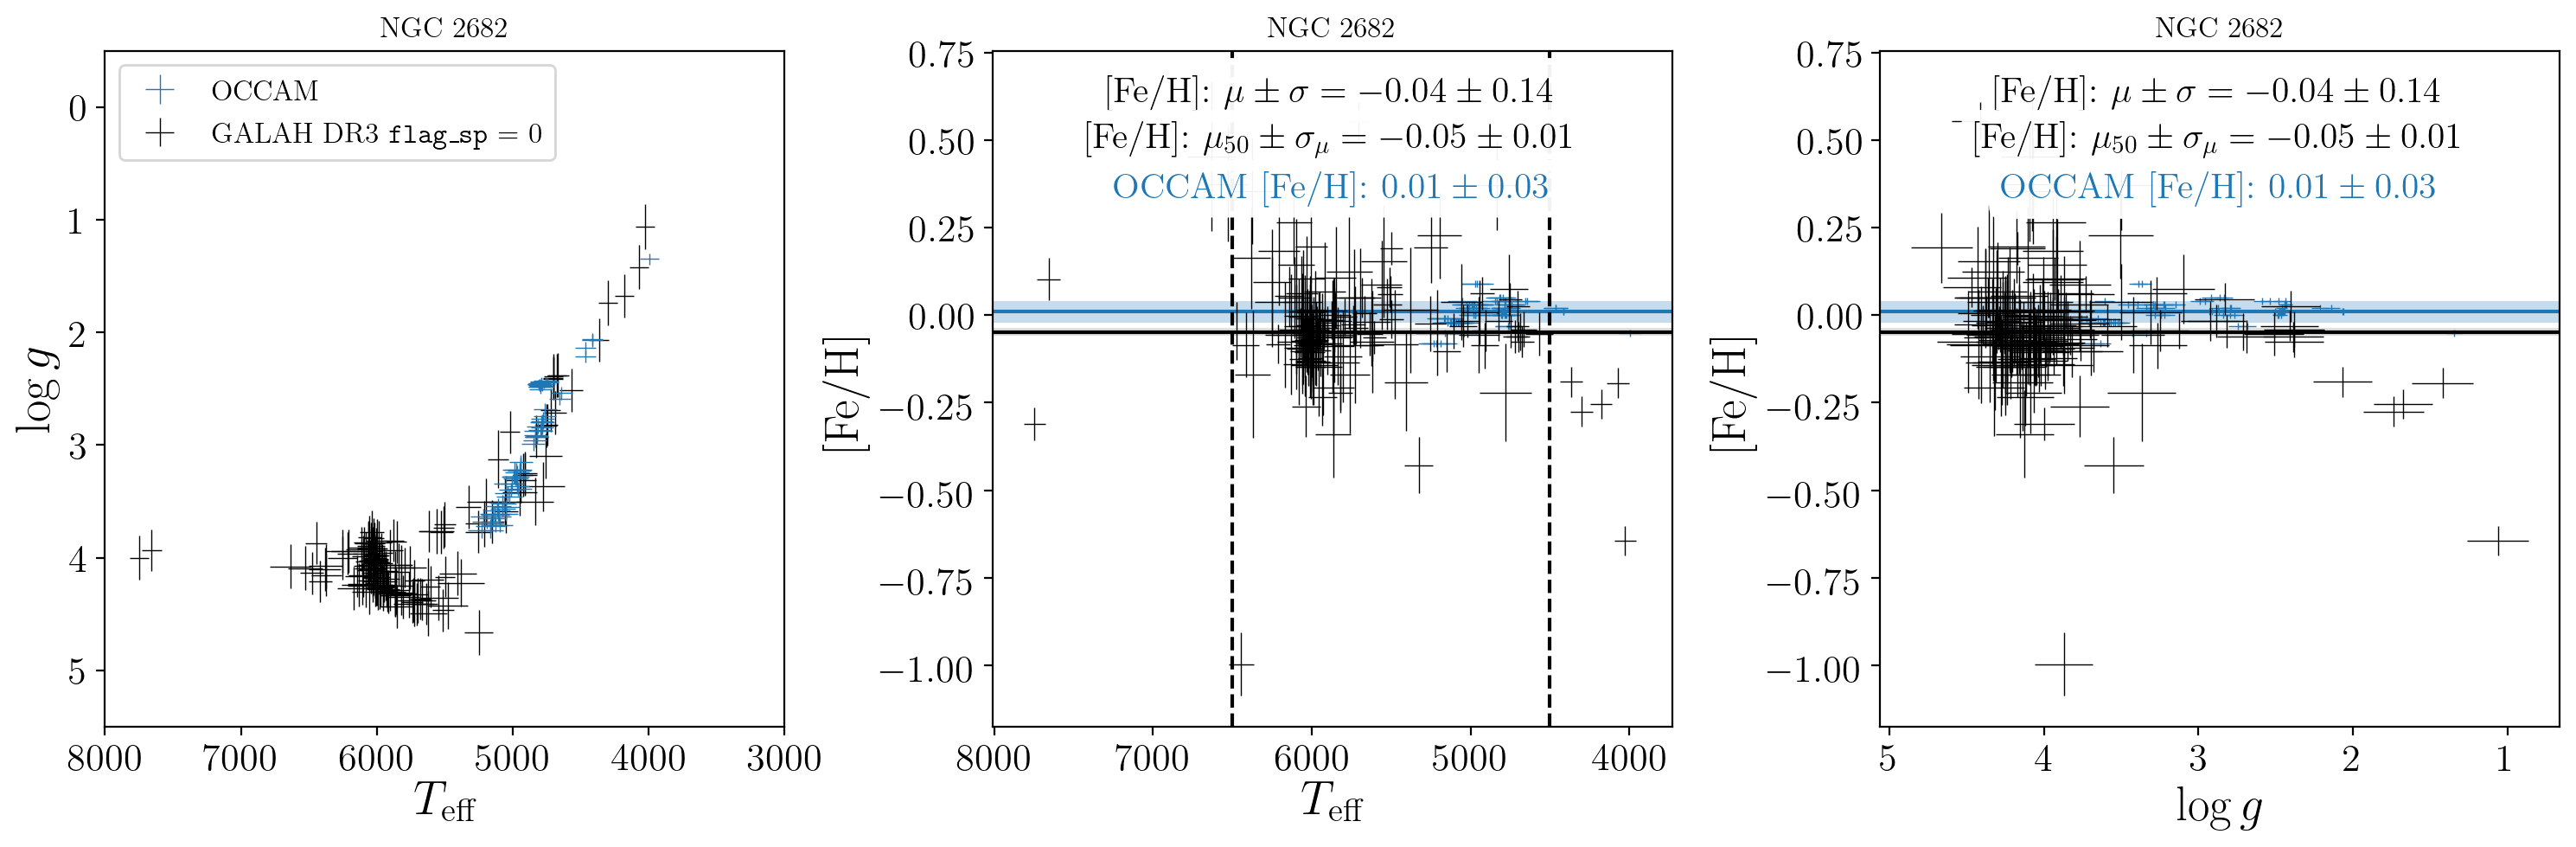
\includegraphics[width=\textwidth]{figures/oc_NGC_2682.png}
%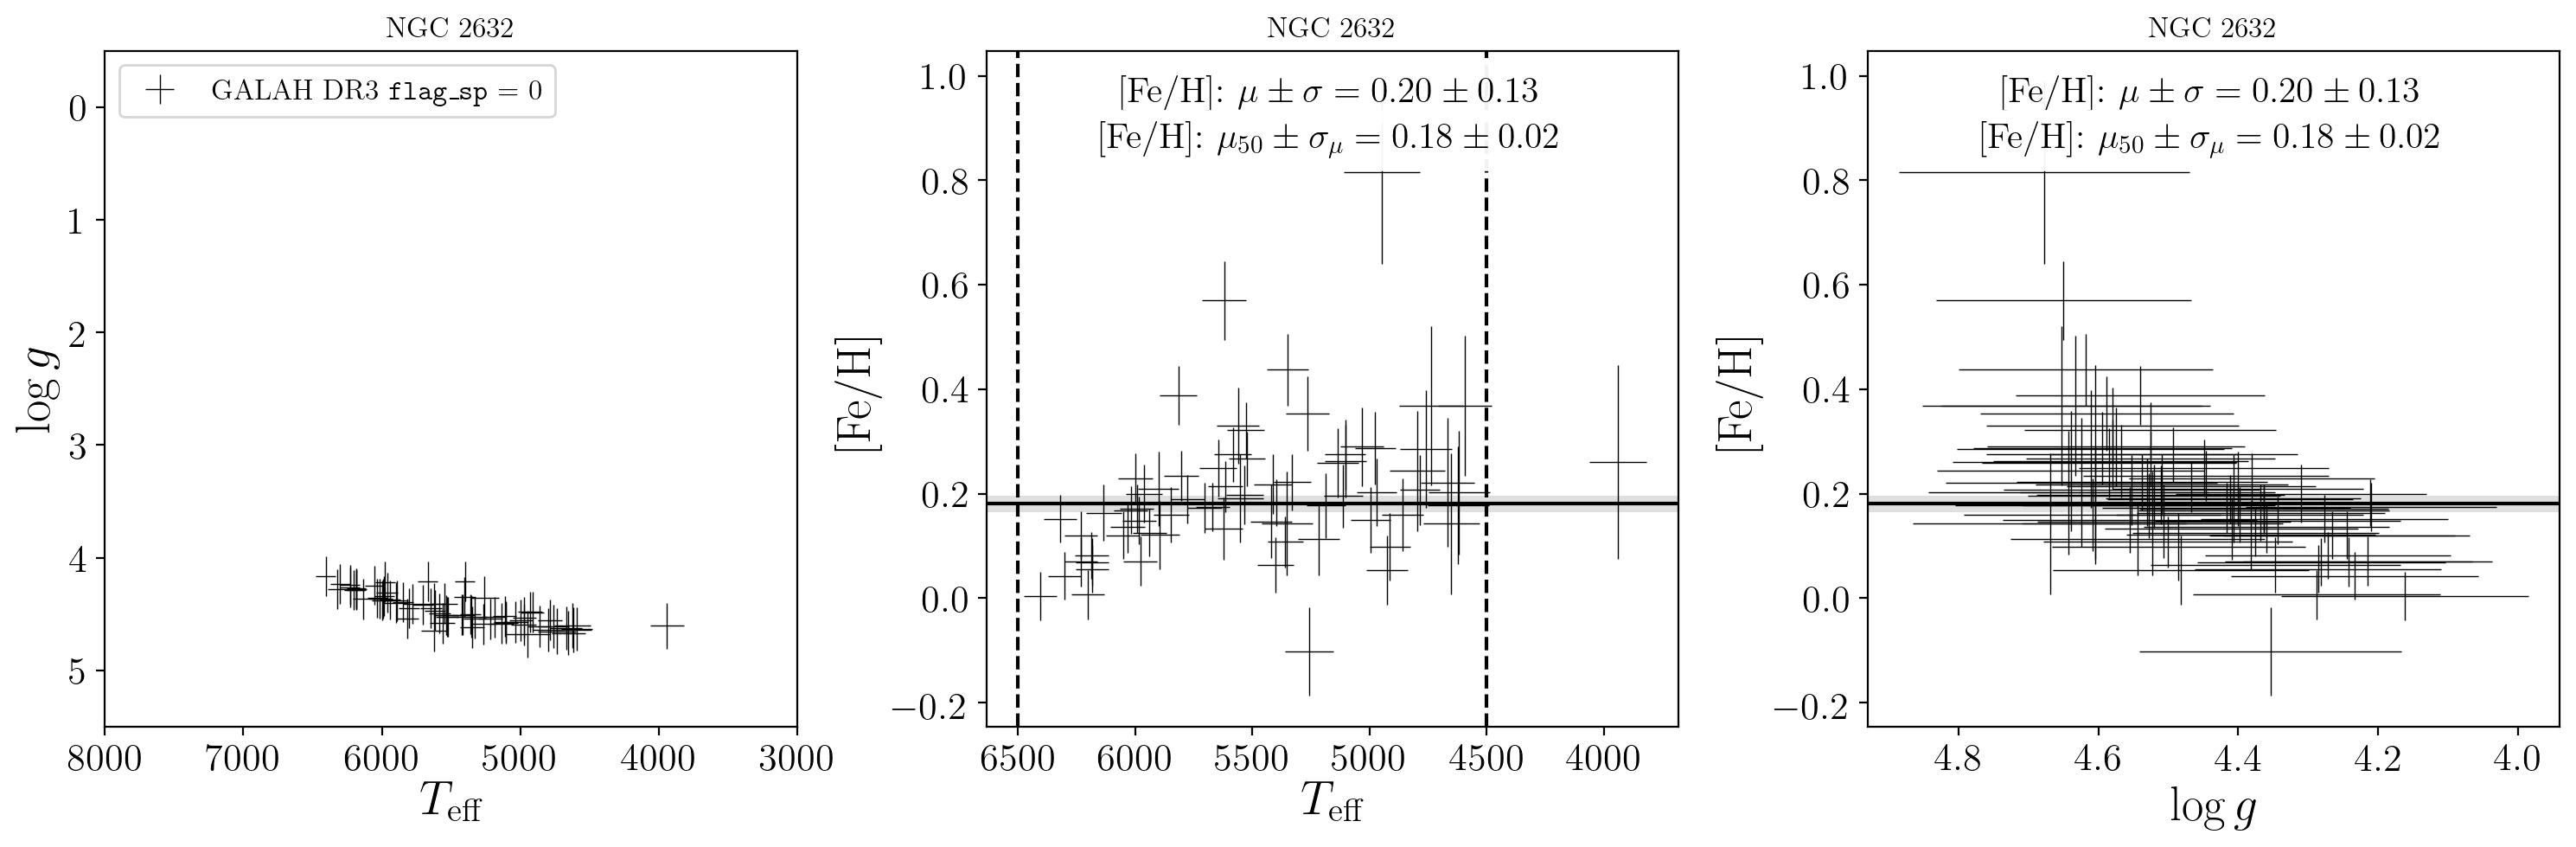
\includegraphics[width=0.49\textwidth]{figures/oc_NGC_2632.png}
%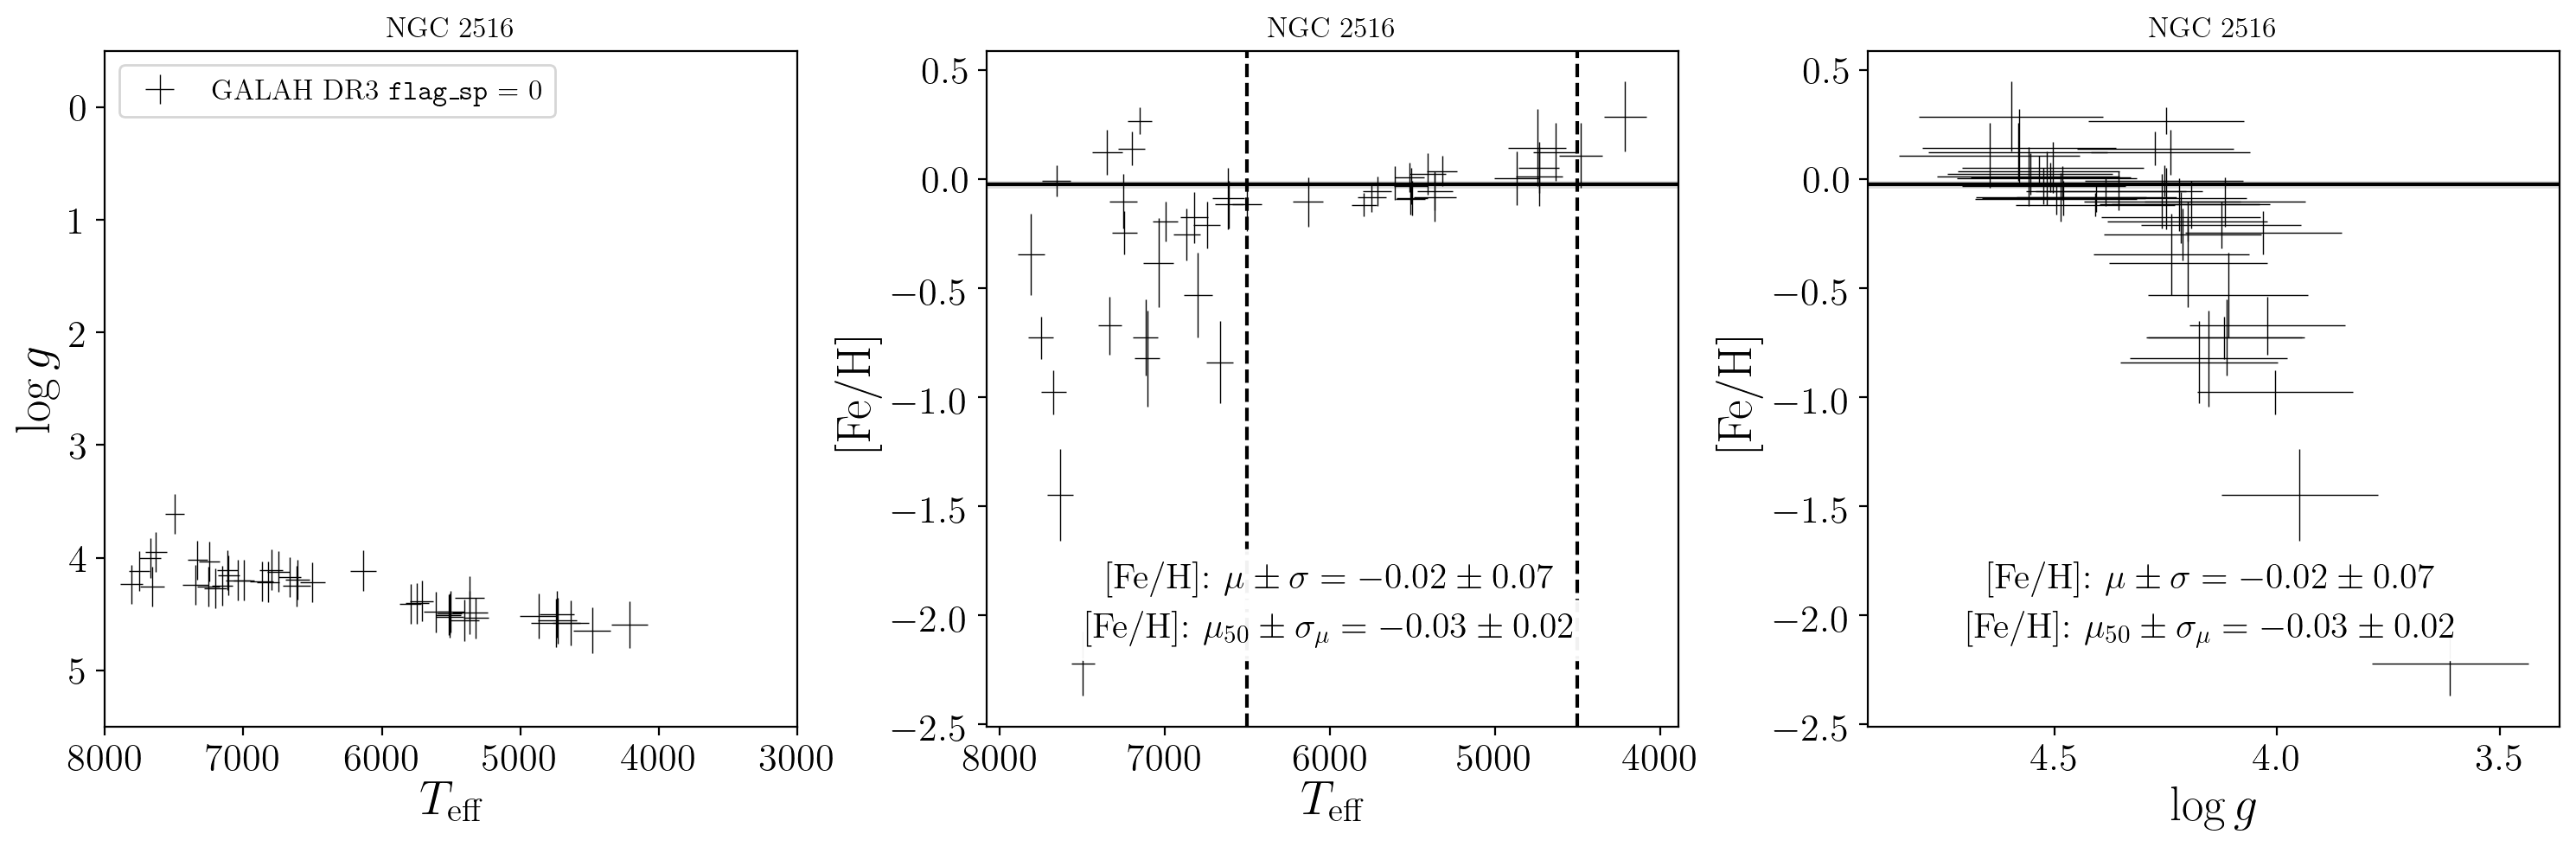
\includegraphics[width=0.49\textwidth]{figures/oc_NGC_2516.png}
%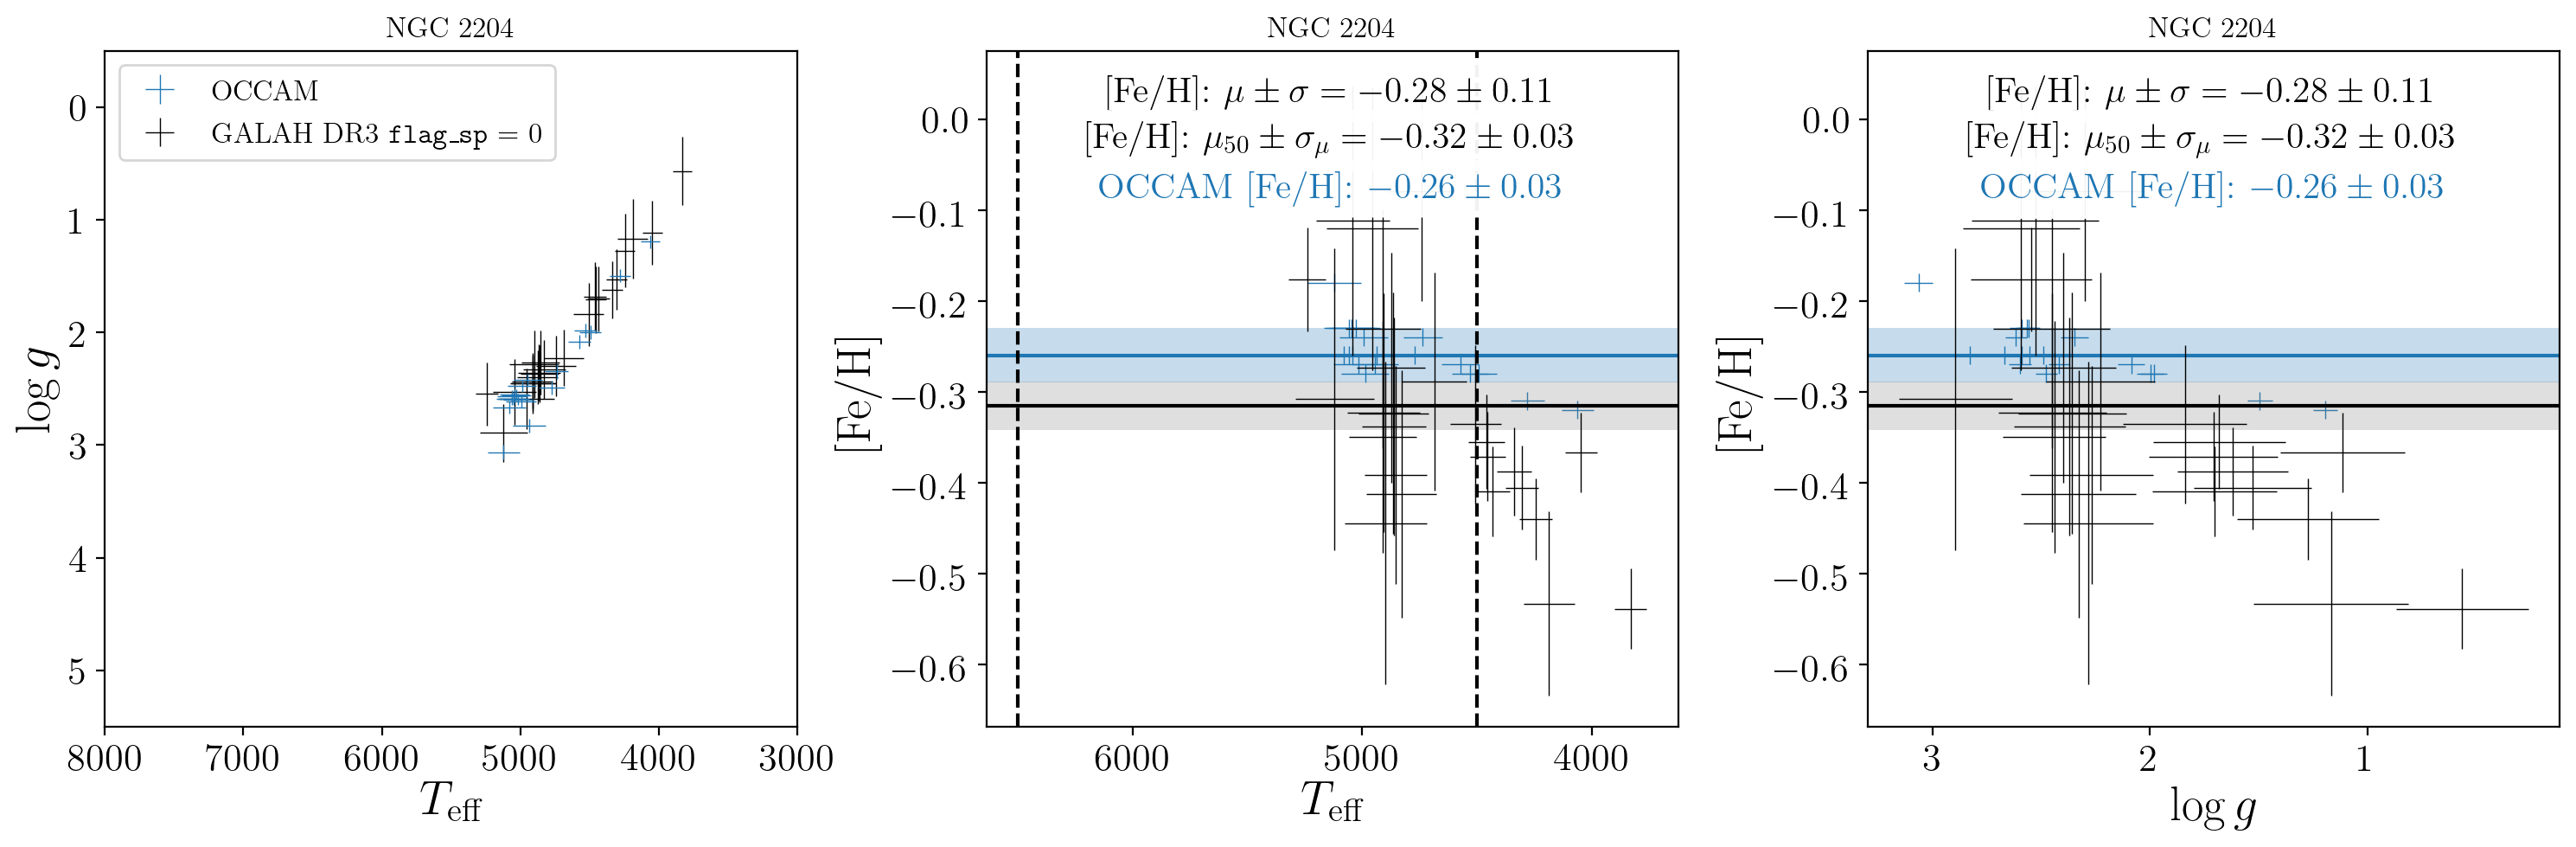
\includegraphics[width=0.49\textwidth]{figures/oc_NGC_2204.png}
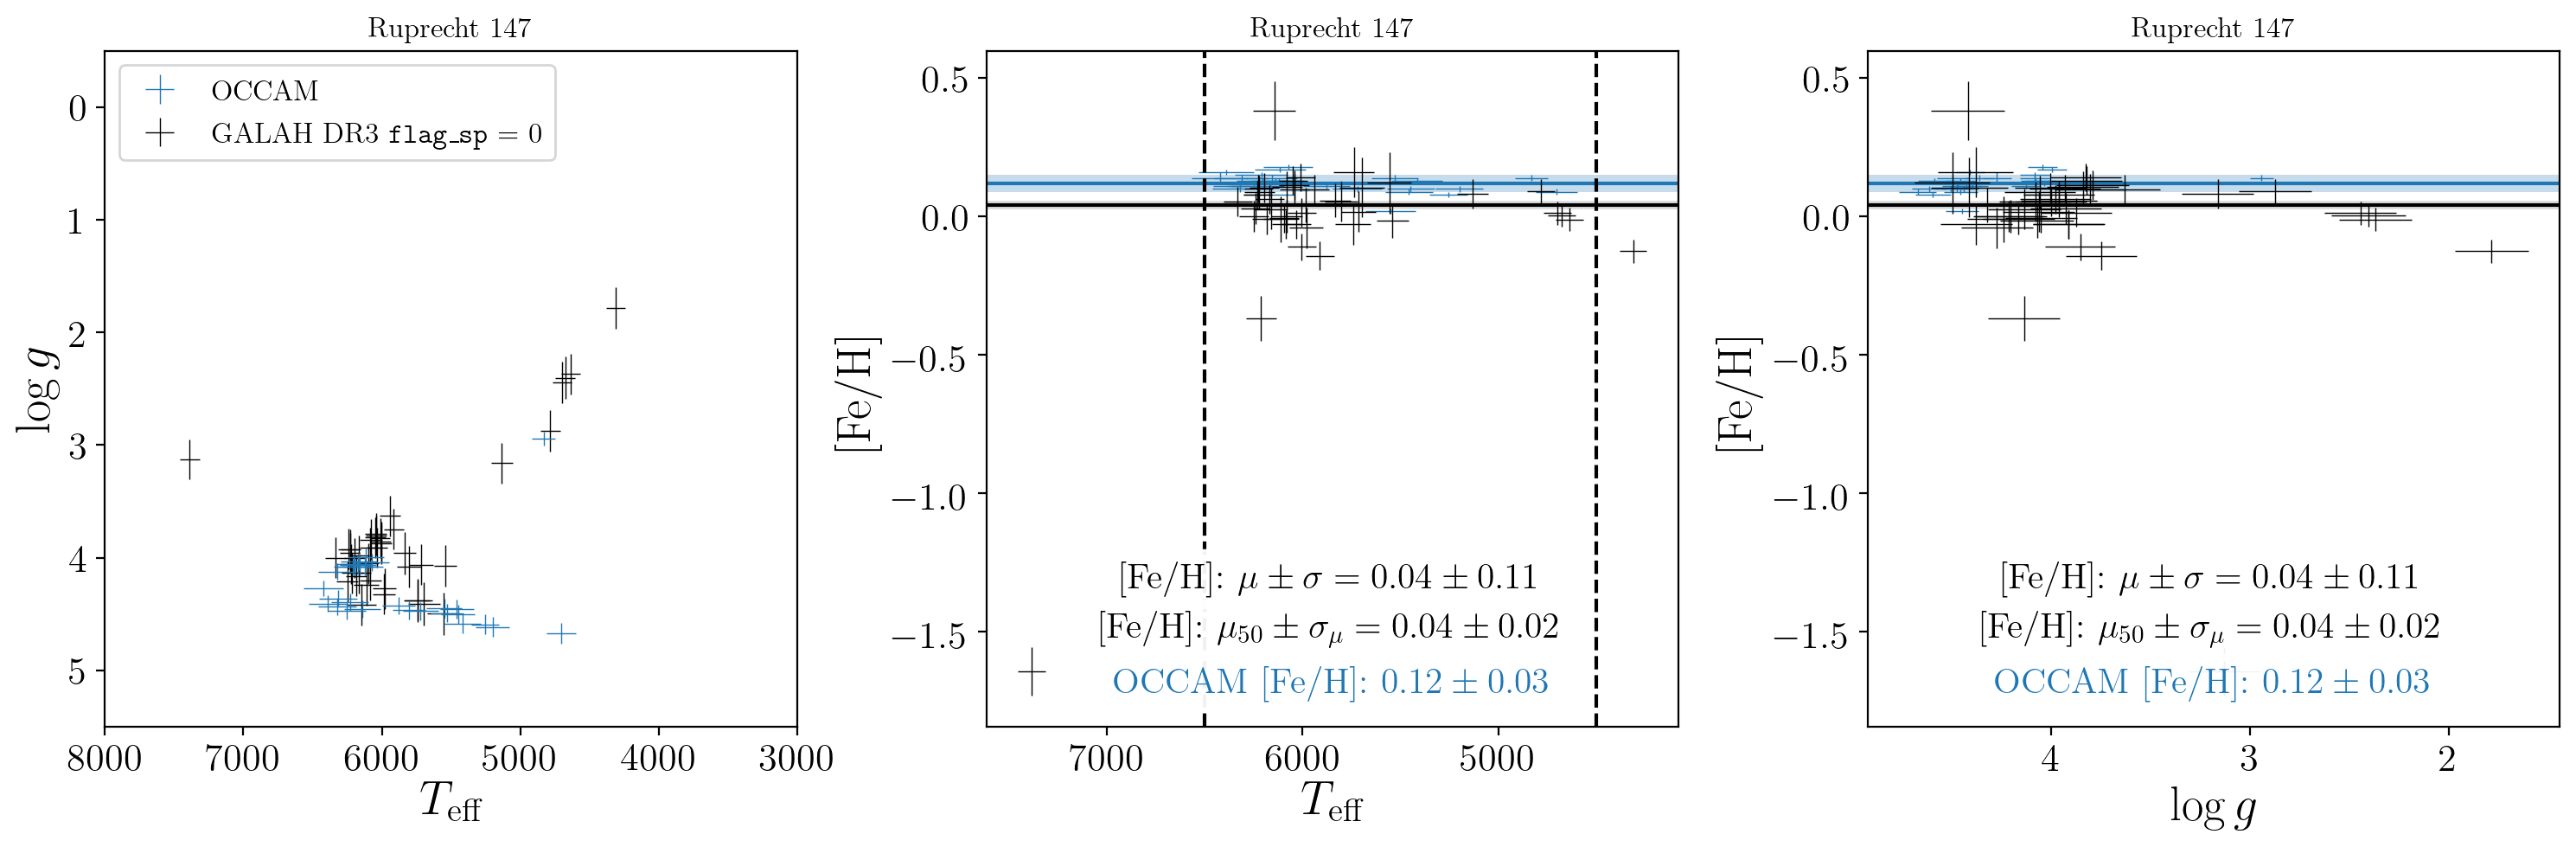
\includegraphics[width=\textwidth]{figures/oc_Ruprecht_147.png}
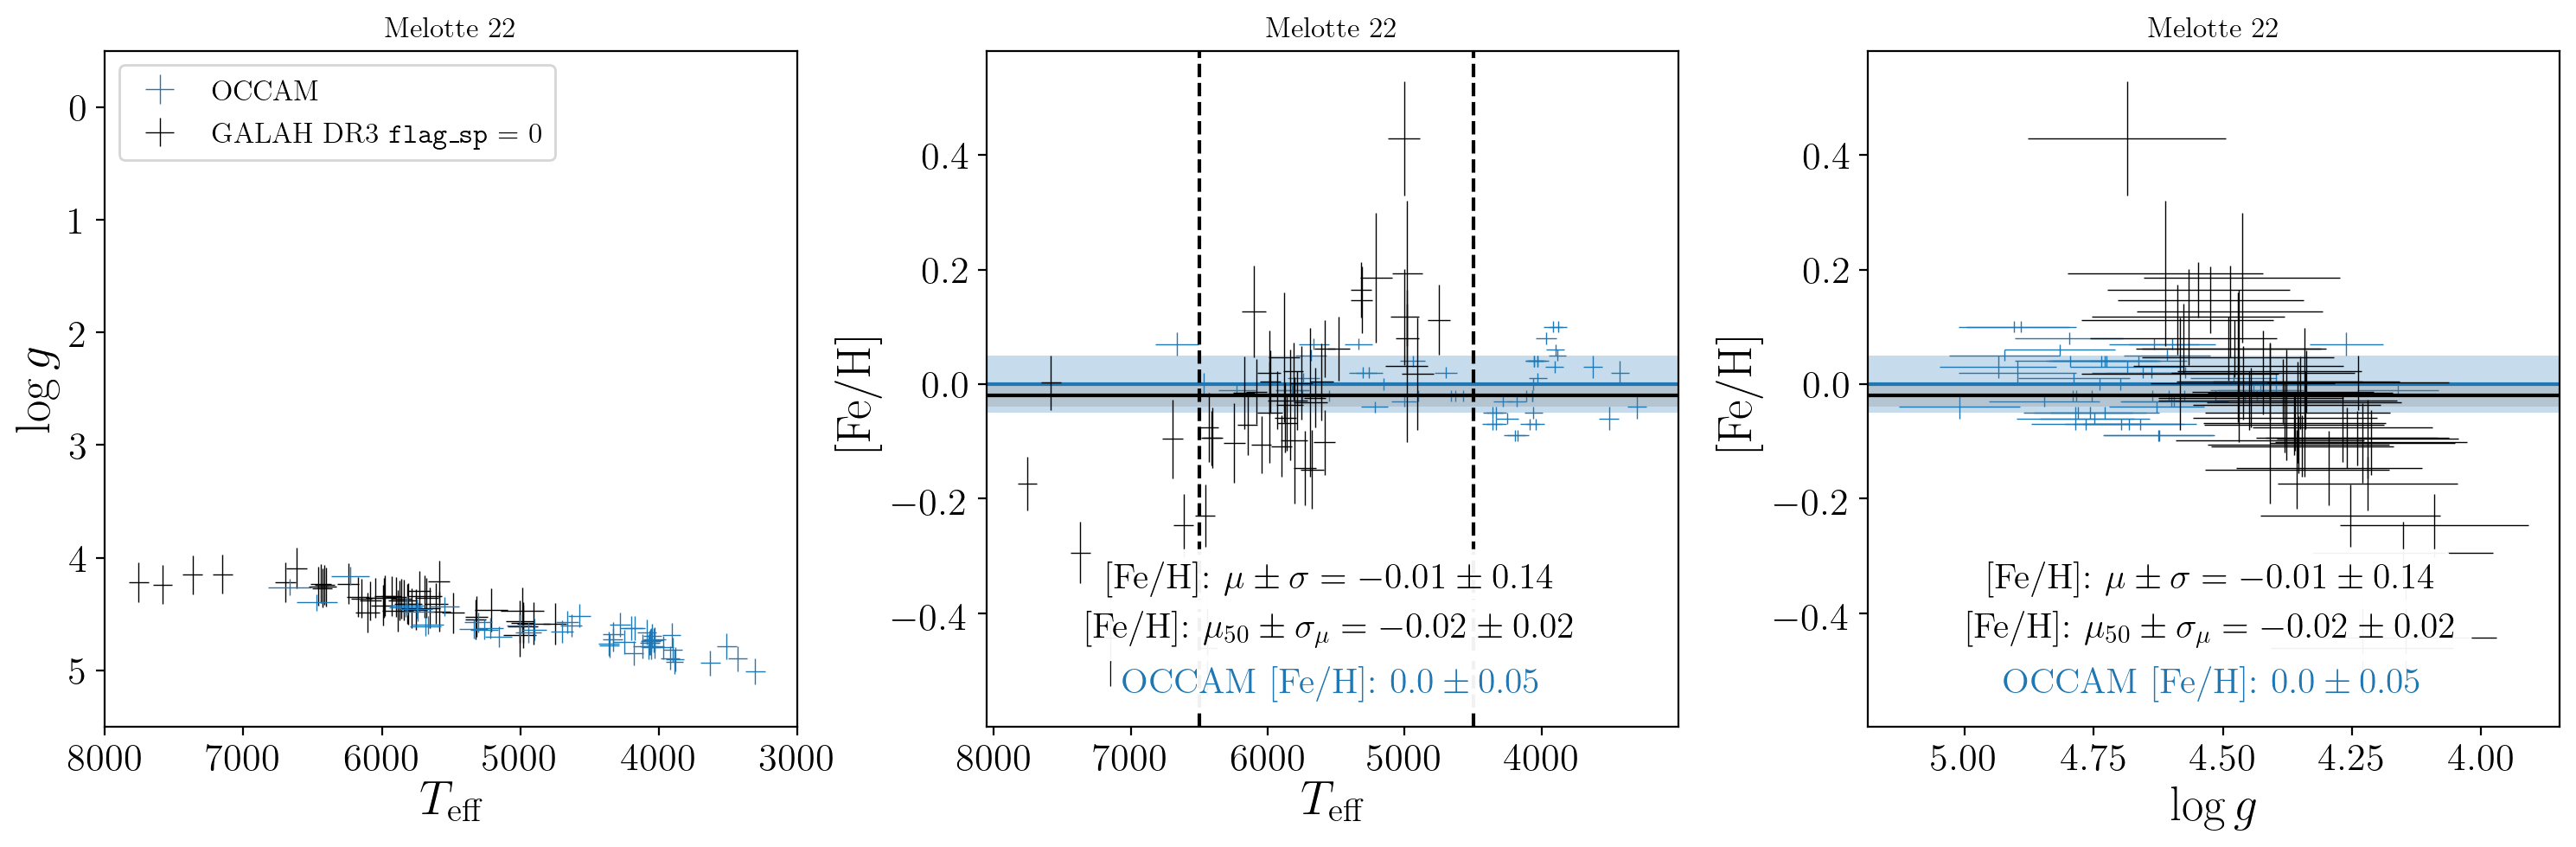
\includegraphics[width=\textwidth]{figures/oc_Melotte_22.png}
%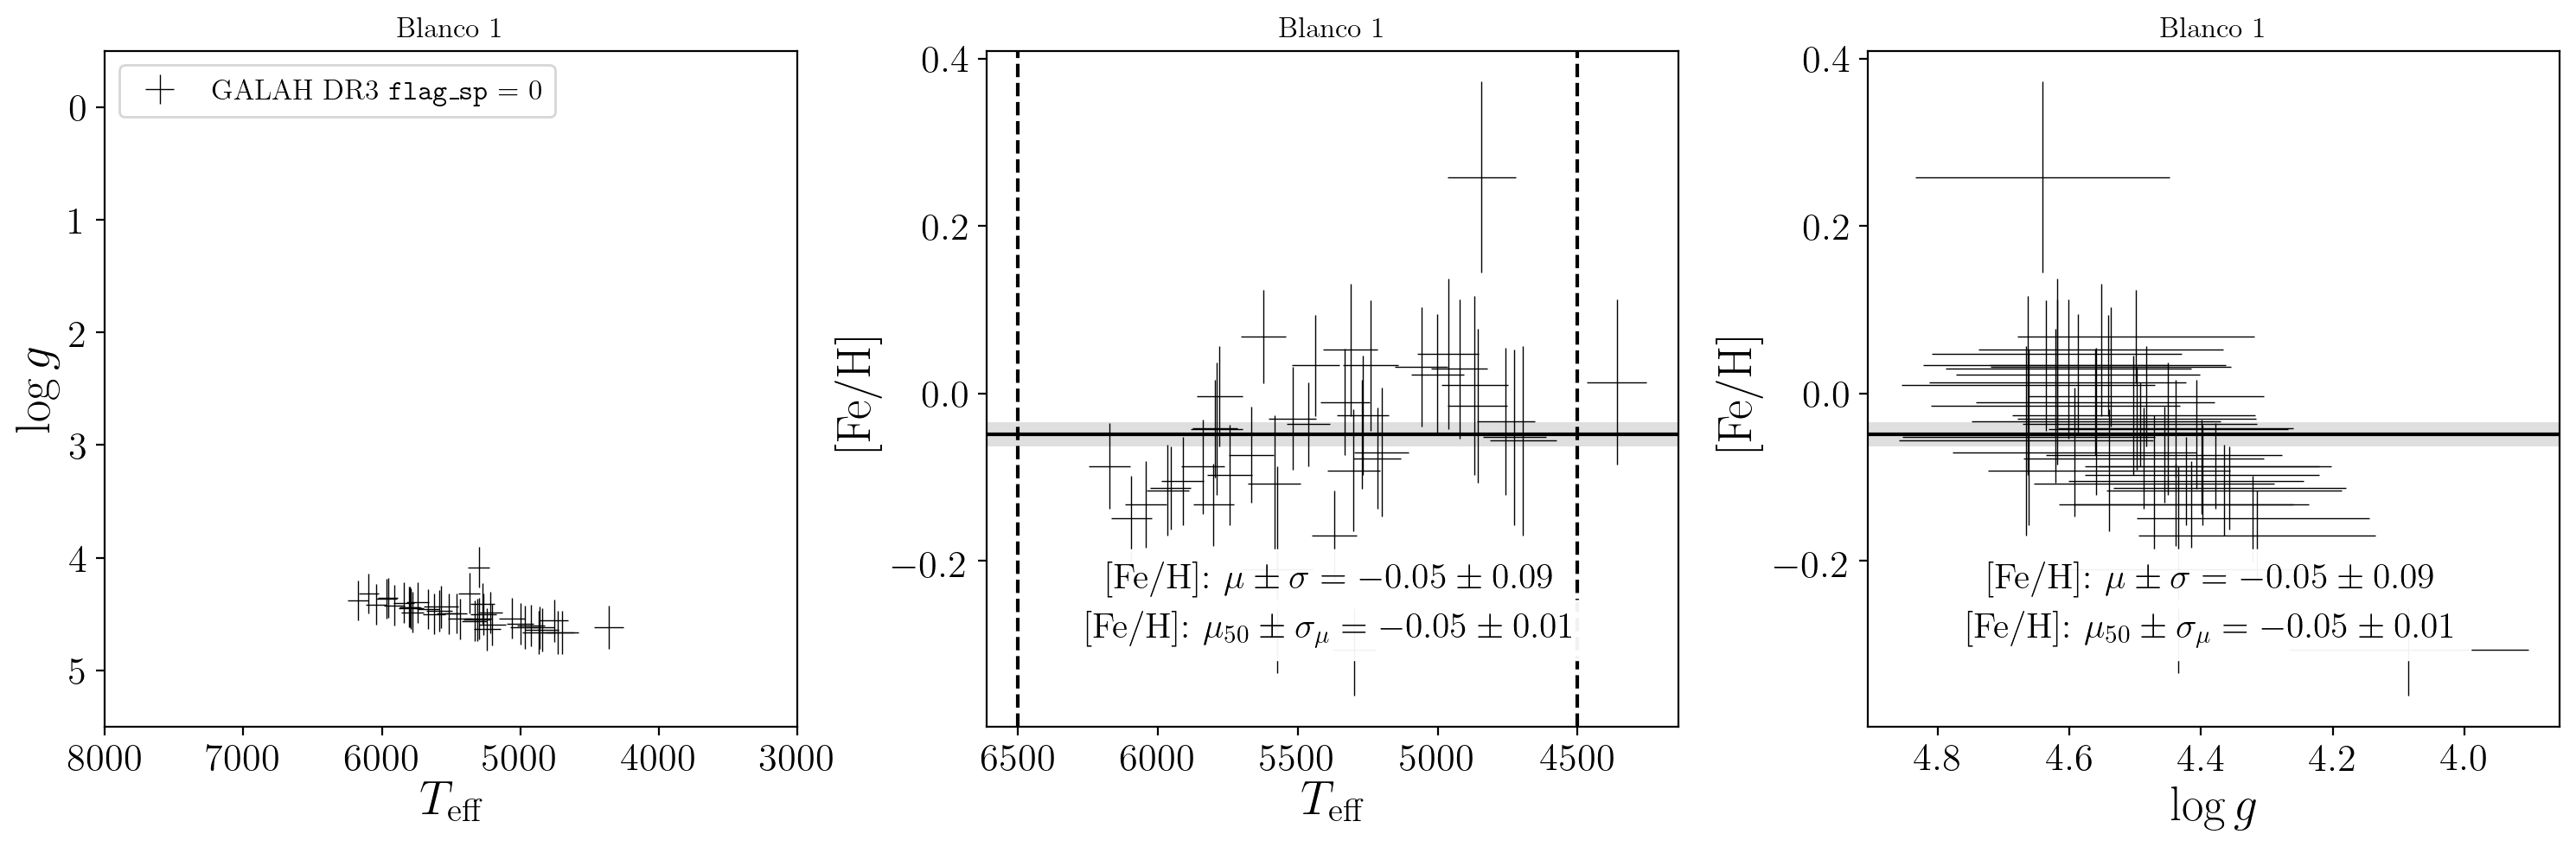
\includegraphics[width=0.49\textwidth]{figures/oc_Blanco_1.png}
%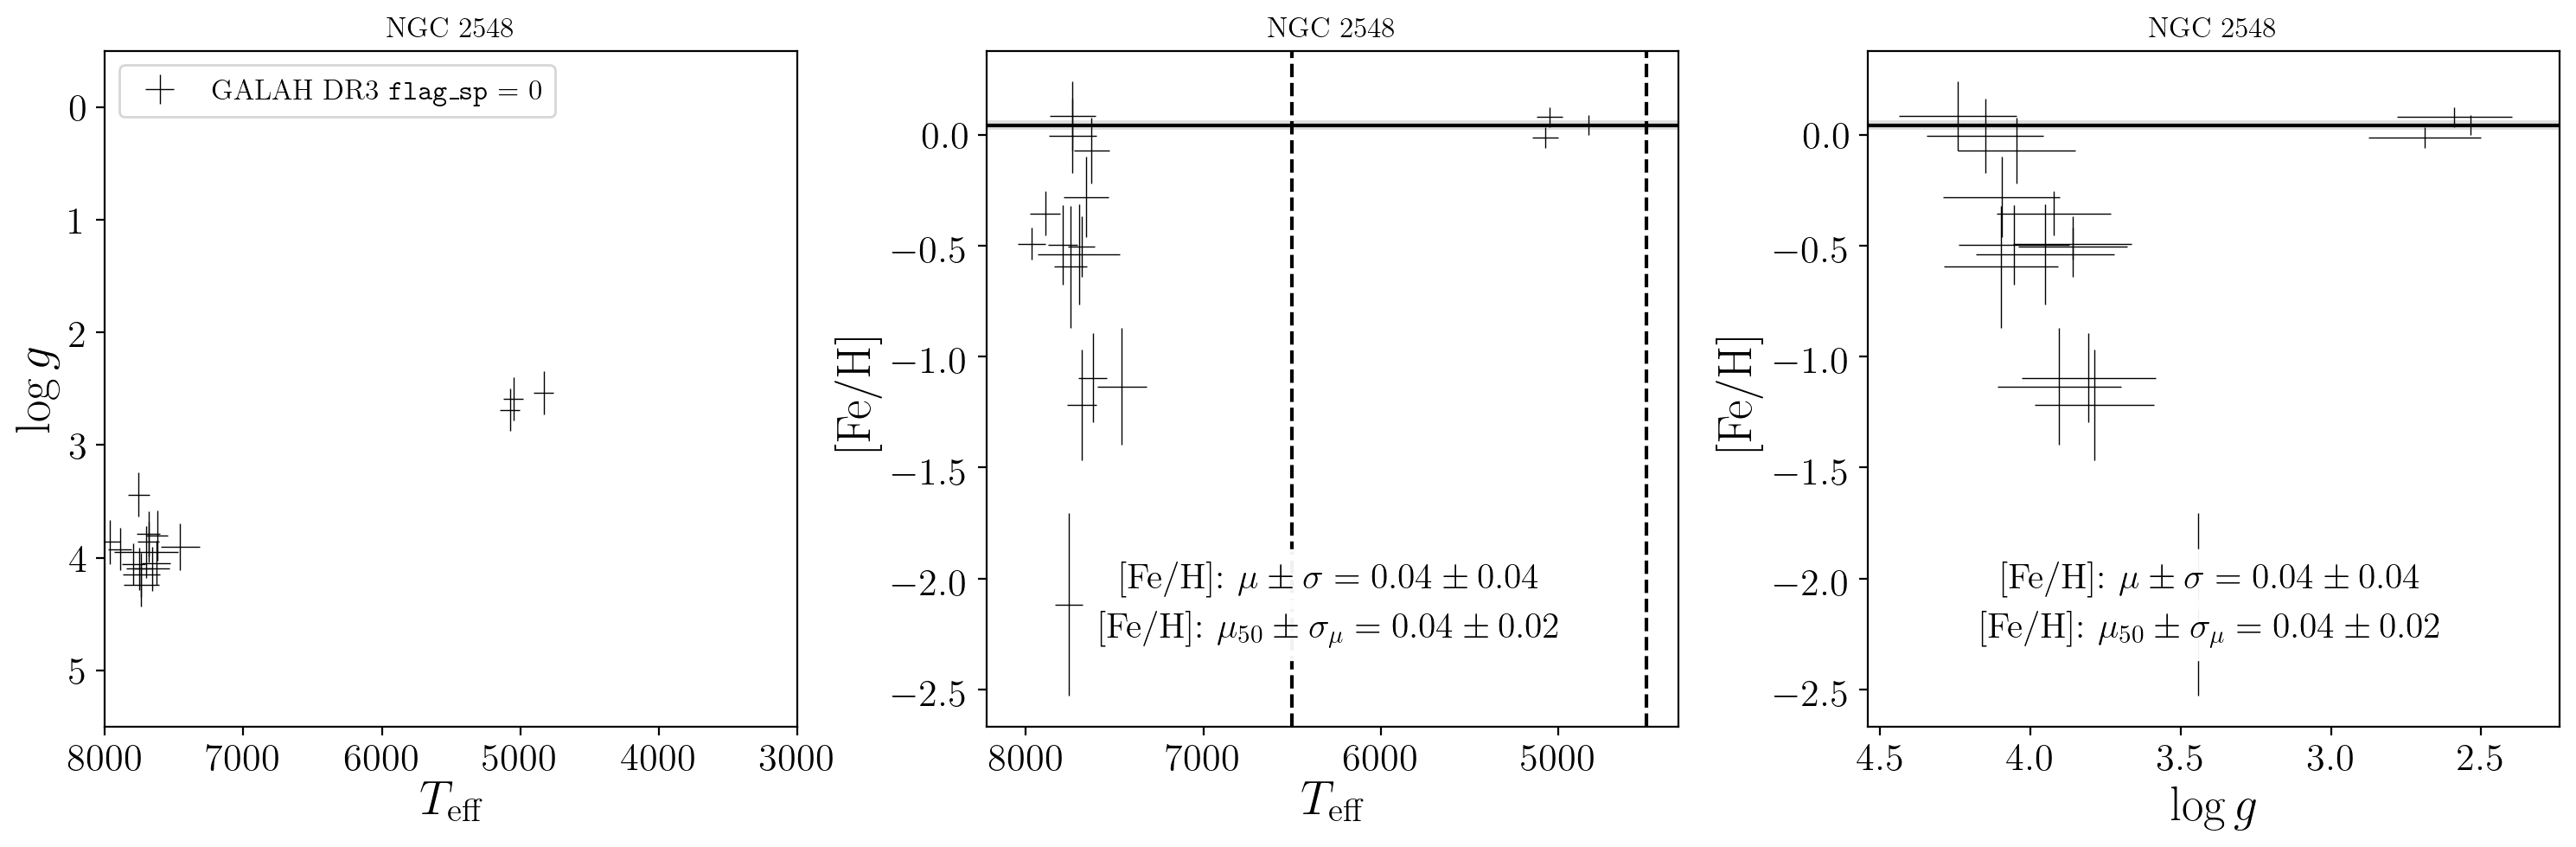
\includegraphics[width=0.49\textwidth]{figures/oc_NGC_2548.png}
%\caption{Stellar parameters (combinations of \Teff, \logg, and \feh) of the eight open clusters NGC~2682 (278 spectra, M~67), NGC~2632 (117, M44, Praesepe), NGC~2516 (83), NGC~2204 (81), Ruprecht~147 (80), Melotte~22 (74), Blanco~1 (67), and NGC~6253 (50) with data from GALAH DR3 (unflagged in black, flagged in red). For four clusters, unflagged data from the OCCAM survey \citep{Donor2020} is plotted in blue in the background. Horizontal bars indicate the mean abundances of the clusters from GALAH in grey (estimated from unflagged measurements of for stars with $4500 < T_\mathrm{eff} < 6500\,\mathrm{K}$) and the OCCAM survey (blue).}
\caption{Stellar parameters (combinations of \Teff, \logg, and \feh) of the three open clusters NGC~2682 (278 spectra, M~67), Ruprecht~147 (80), and Melotte~22  with data from GALAH DR3 (unflagged in black, flagged in red). For four clusters, unflagged data from the OCCAM survey \citep{Donor2020} is plotted in blue in the background. Horizontal bars indicate the mean abundances of the clusters from GALAH in grey (estimated from unflagged measurements of for stars with $4500 < T_\mathrm{eff} < 6500\,\mathrm{K}$) and the OCCAM survey (blue).}
\label{fig:oc_stellar_params}
\end{figure*}

% Created with GALAH_DR3/validation/comparisons/comparison_clusters/GALAH_DR3_Comparison_Clusters.ipynb
\begin{figure*}
\centering
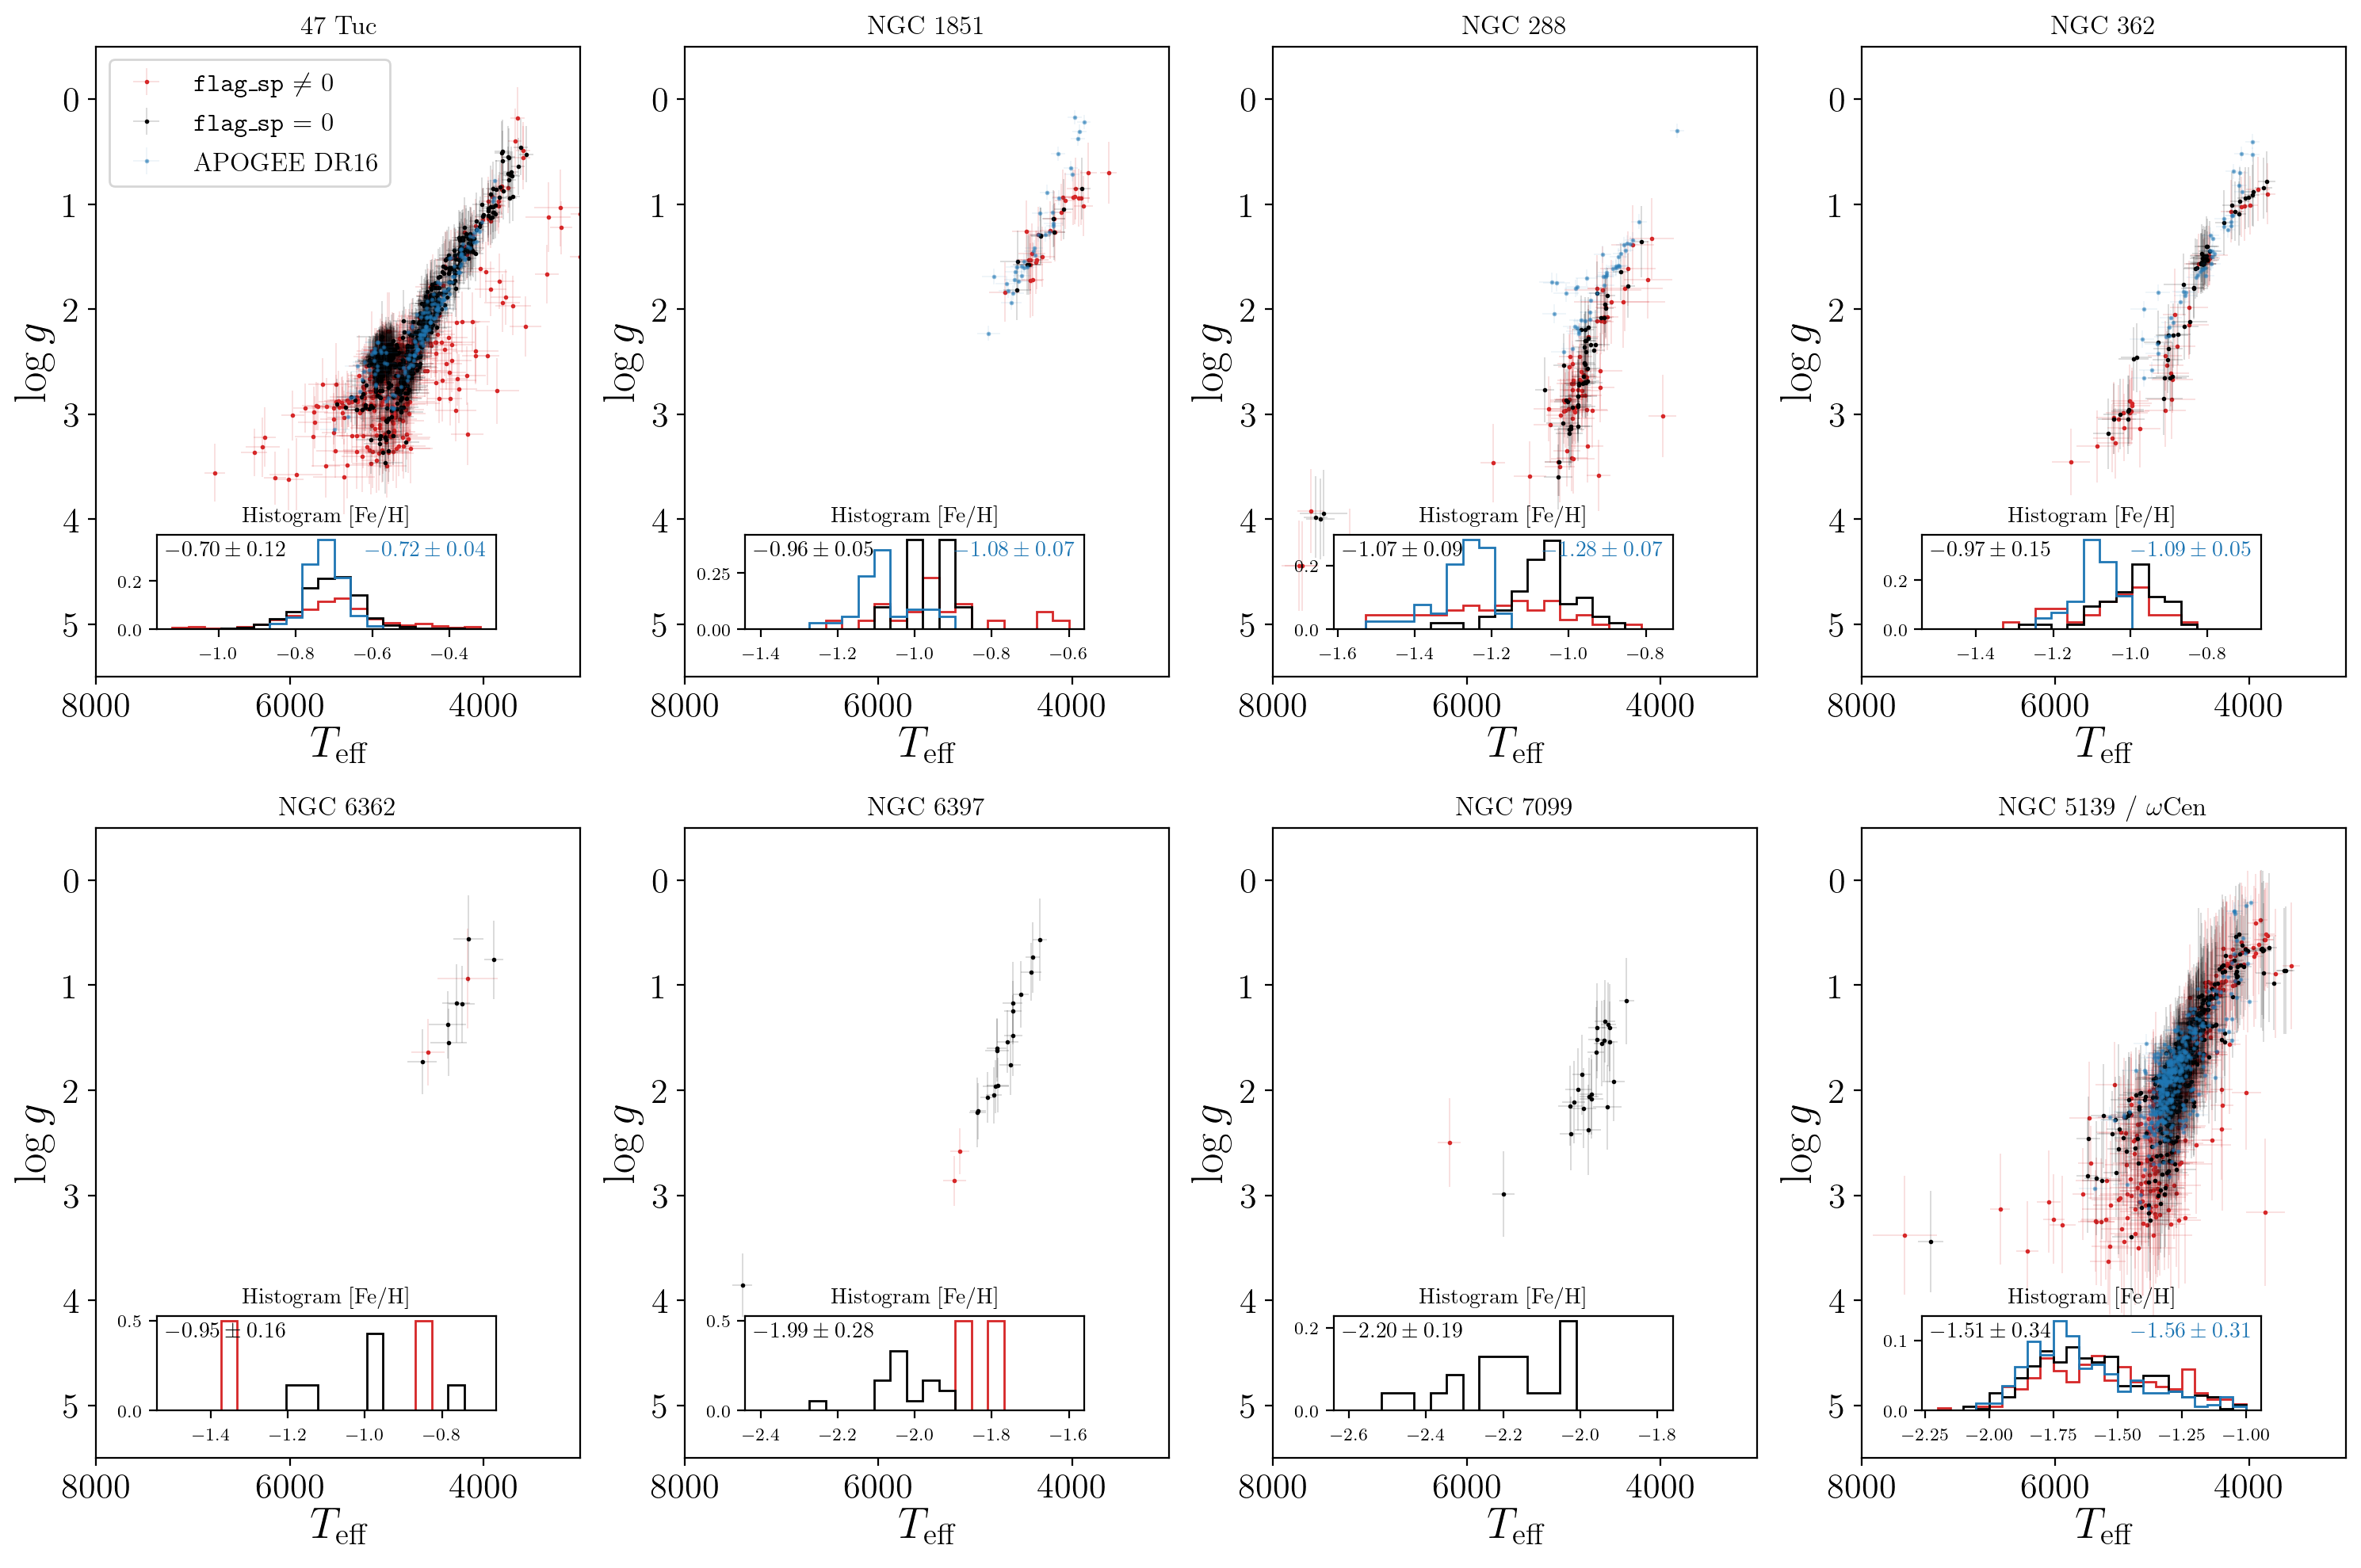
\includegraphics[width=\textwidth]{figures/gc_kiel_diagrams.png}
\caption{Kiel diagrams (\Teff vs. \logg) for eight globular clusters observed by GALAH (unflagged in black, flagged in red). For five clusters, unflagged data from APOGEE DR16 survey \citep{SDSSDR16} is plotted in blue. Inset plots in each panel indicate the normalised [Fe/H] distribution of the shown stars with text annotating the simple mean and standard deviations of the observed stars.}
\label{fig:gc_feh}
\end{figure*}

\paragraph*{Stellar parameters of wide binaries}

We used the approach by \citet{ElBadry2018c} to select wide binaries \Gaia and further limit the selection to those with similar GALAH DR3 \vrad (within $1\,\mathrm{km/s}$. We find 268 pairs, including dwarf-giant pairs. In Fig.~\ref{fig:wide_binary_sp} we plot the stellar parameters \Teff, \logg, \feh, and \vrad to illustrate the difference of [Fe/H] and \vrad for these stars with sometimes quite different stellar parameters. We want to stress that we include also stars with \texttt{flag\_sp} up to 128 (for example the very cool, flagged stars as well as apparent photometric binary stars with unreliable \logg). As previous studies have shown \citep{ElBadry2018b, ElBadry2018c}, we expect very similar abundances for these pairs and indeed can confirm that their \feh and \vrad are consistent within the uncertainties for almost all cases. The average differences of $\Delta v_\text{rad} = -0.05 \pm 0.41\,\mathrm{km/s}$ and $\Delta \mathrm{[Fe/H]} = -0.01 \pm 0.08\,\mathrm{dex}$ show excellent agreement over large scales (when neglecting the 8 outliers of 268 pairs, shown in red). We furthermore do not see significant trends of the differences of \feh with \Teff, \logg, \feh, or \vrad, which lends confidence that our analysis is reliable within the stellar parameter range of the observed wide binaries. Even most of the dwarf-giant pairs show a very good agreement.

\begin{figure*}
\centering
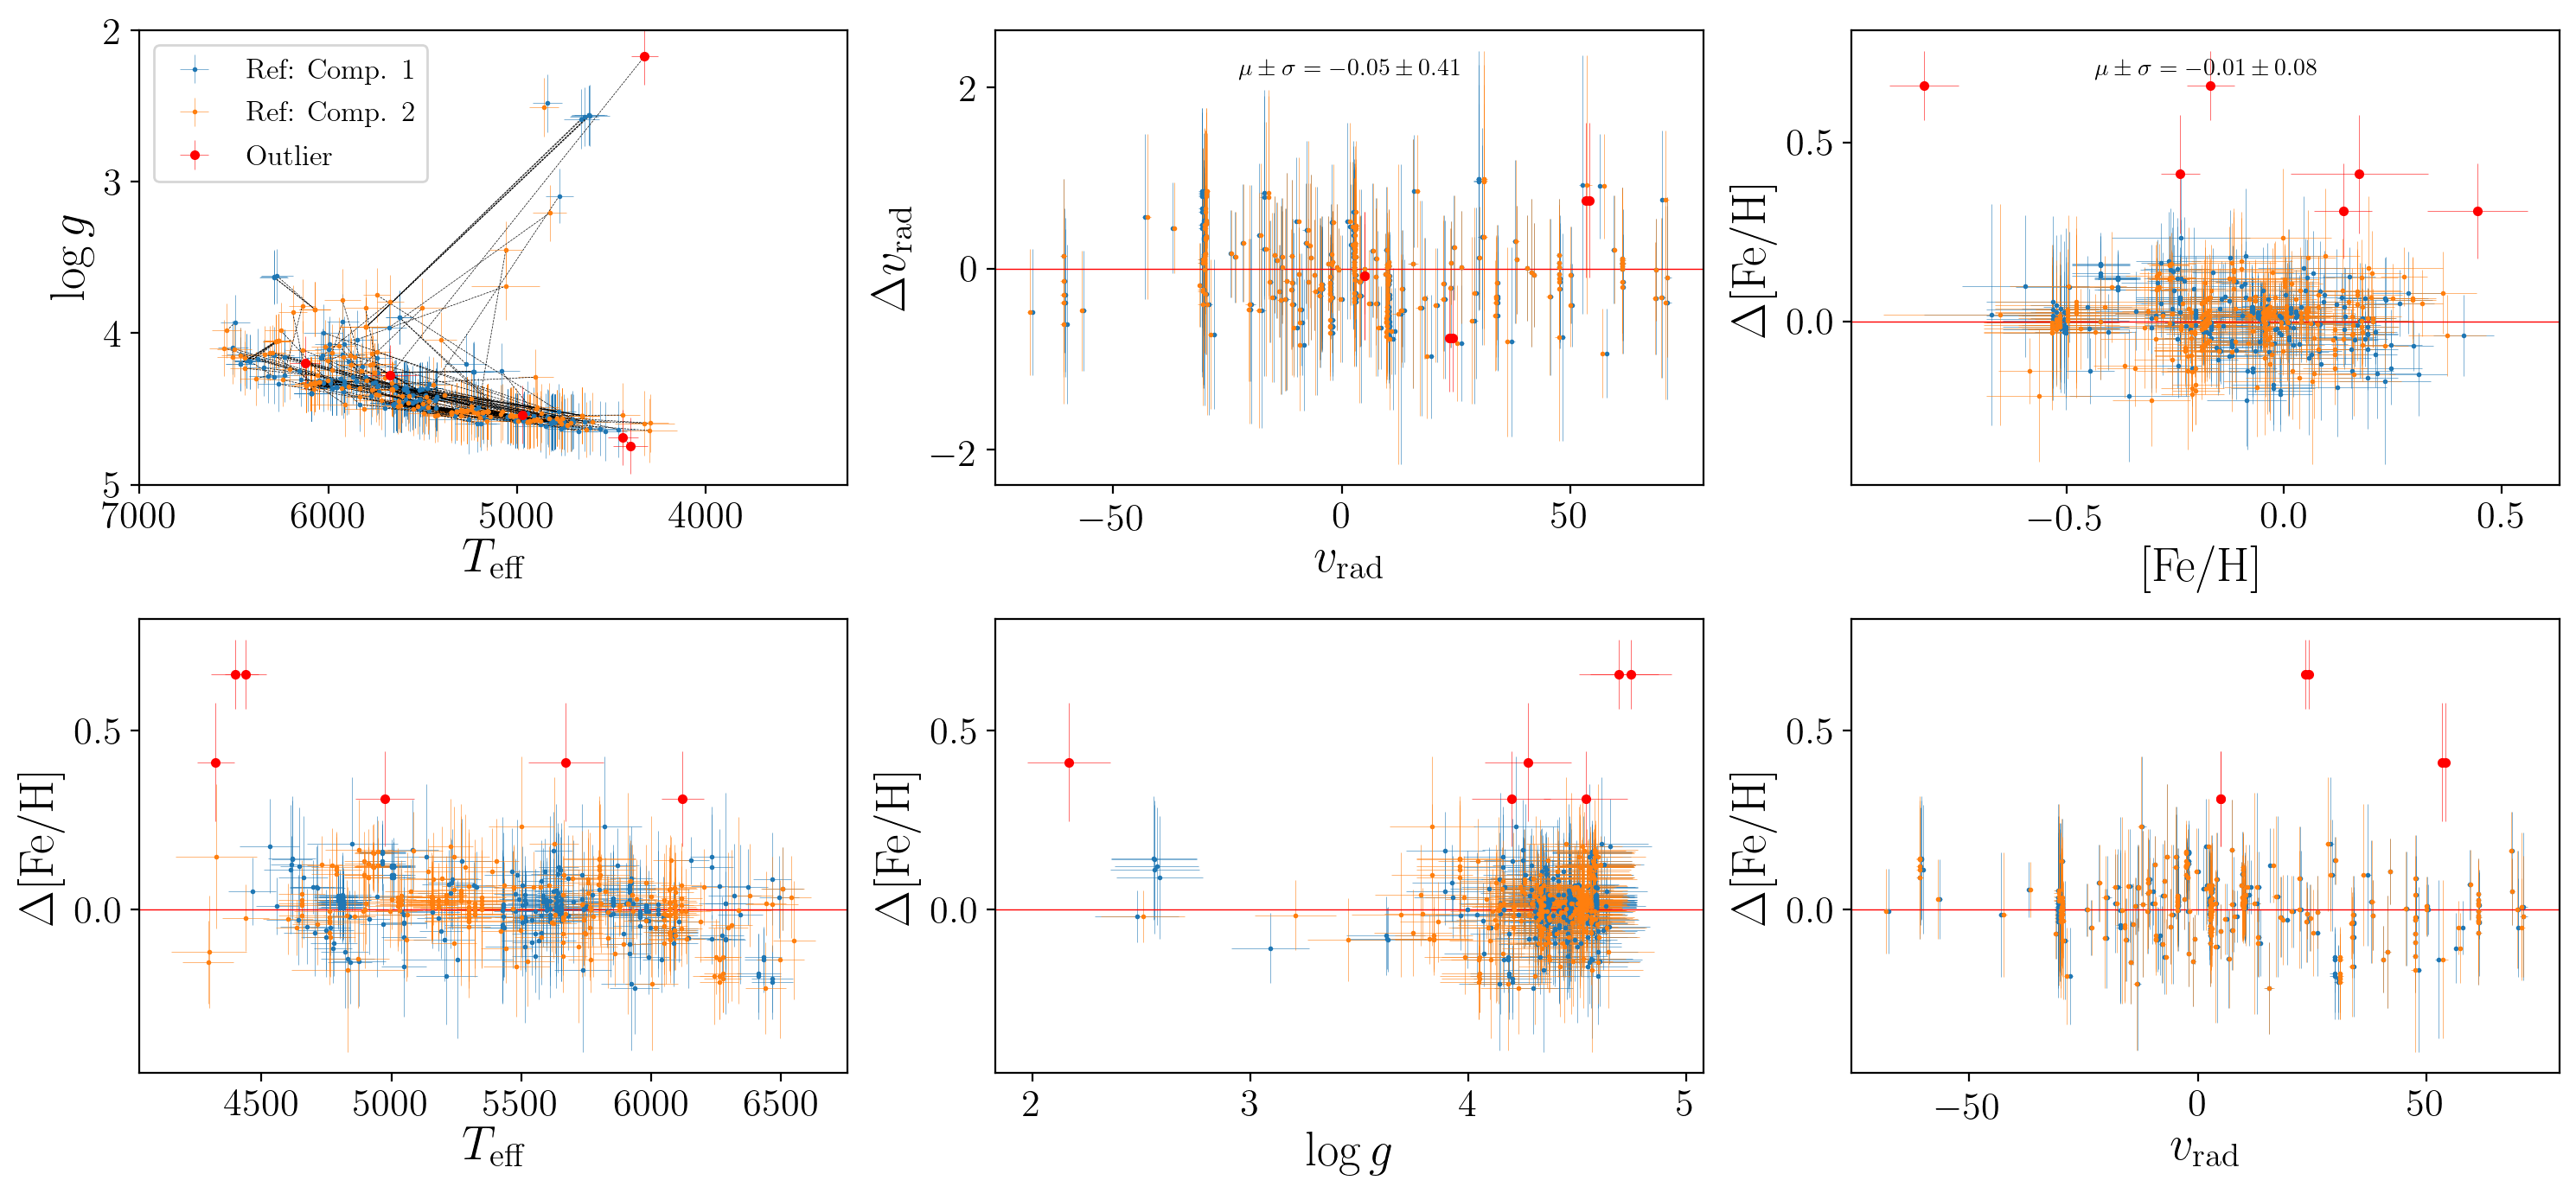
\includegraphics[width=\textwidth]{figures/wide_binaries_sp.png}
\caption{Comparison of stellar parameters \Teff, \logg, \feh, and \vrad for wide binaries identified with the algorithm by \citet{ElBadry2018c}. We plot different combinations of these parameters as references (blue for component 1 and orange for component 2) and asses the difference in \feh and \vrad. We include stars with \texttt{flag\_sp} up to 128.}
\label{fig:wide_binary_sp}
\end{figure*}

\subsection{Flagging of stellar parameters} \label{sec:flagging_sp}

After the stellar parameters have been estimated, we raise flags according to the individual criteria listed in Table~\ref{tab:flag_sp_galah_dr3}. Fig.~\ref{fig:hrd_galah_dr3} shows all those spectra with raised flags. The most used flags are 8 (7\%), 1 (6\%) and 4 (3\%). \SB{Update once final catalog is on WIKI.}

\begin{table}
\centering
 \caption{Flags used for GALAH DR3 to estimate the final bit-flag \texttt{flag\_sp} via summation of the individual flags.}
 \label{tab:flag_sp_galah_dr3}
 \begin{tabular}{rl}
  \hline \hline
Flag		&	Description	\\
\hline
   1	&	\Gaia RUWE > 1.4 \\
   	&	\citep[unreliable astrometric solution, see][]{Lindegren2018b} \\
   2	&	Unreliable broadening \\
   4	&	Low S/N (below 10 for CCD 2) \\
   8	&	Reduction issues \\
	&	a) Wavelength solution (propagating of \texttt{red\_flag}), \\
	&	b) t-SNE projected reduction issues, \\
	&	c) Negative/positive fluxes, spikes, etc. \\
  16	&	t-SNE projected emission features \\
  32	&	t-SNE projected binaries \\
  64	&	Binary sequence/pre-main sequence flag \\
 128	&	SNR-dependent high {\sc sme} chi2 (bad fit) \\
 256	&	Problems with Fe lines, where line flux is \\
 	&	not between 0.03 and 1.00 \\
 512	&	{\sc sme} did not finish \\
     	&	a) No convergence == non-finite stellar parameters \\
   	&	b) Gaussian RV fit failed \\
     	&	c) Timeout on ISAAC \\
1024	&	{\sc marcs} grid limit reached or \\
	&	outside of reasonable parameter range \\
  \hline
 \end{tabular}
\end{table}

% This figure was created with GALAH_DR3/validation/stellar_parameters/overview/stellar_parameter_overview.ipynb
\begin{figure*}
\centering
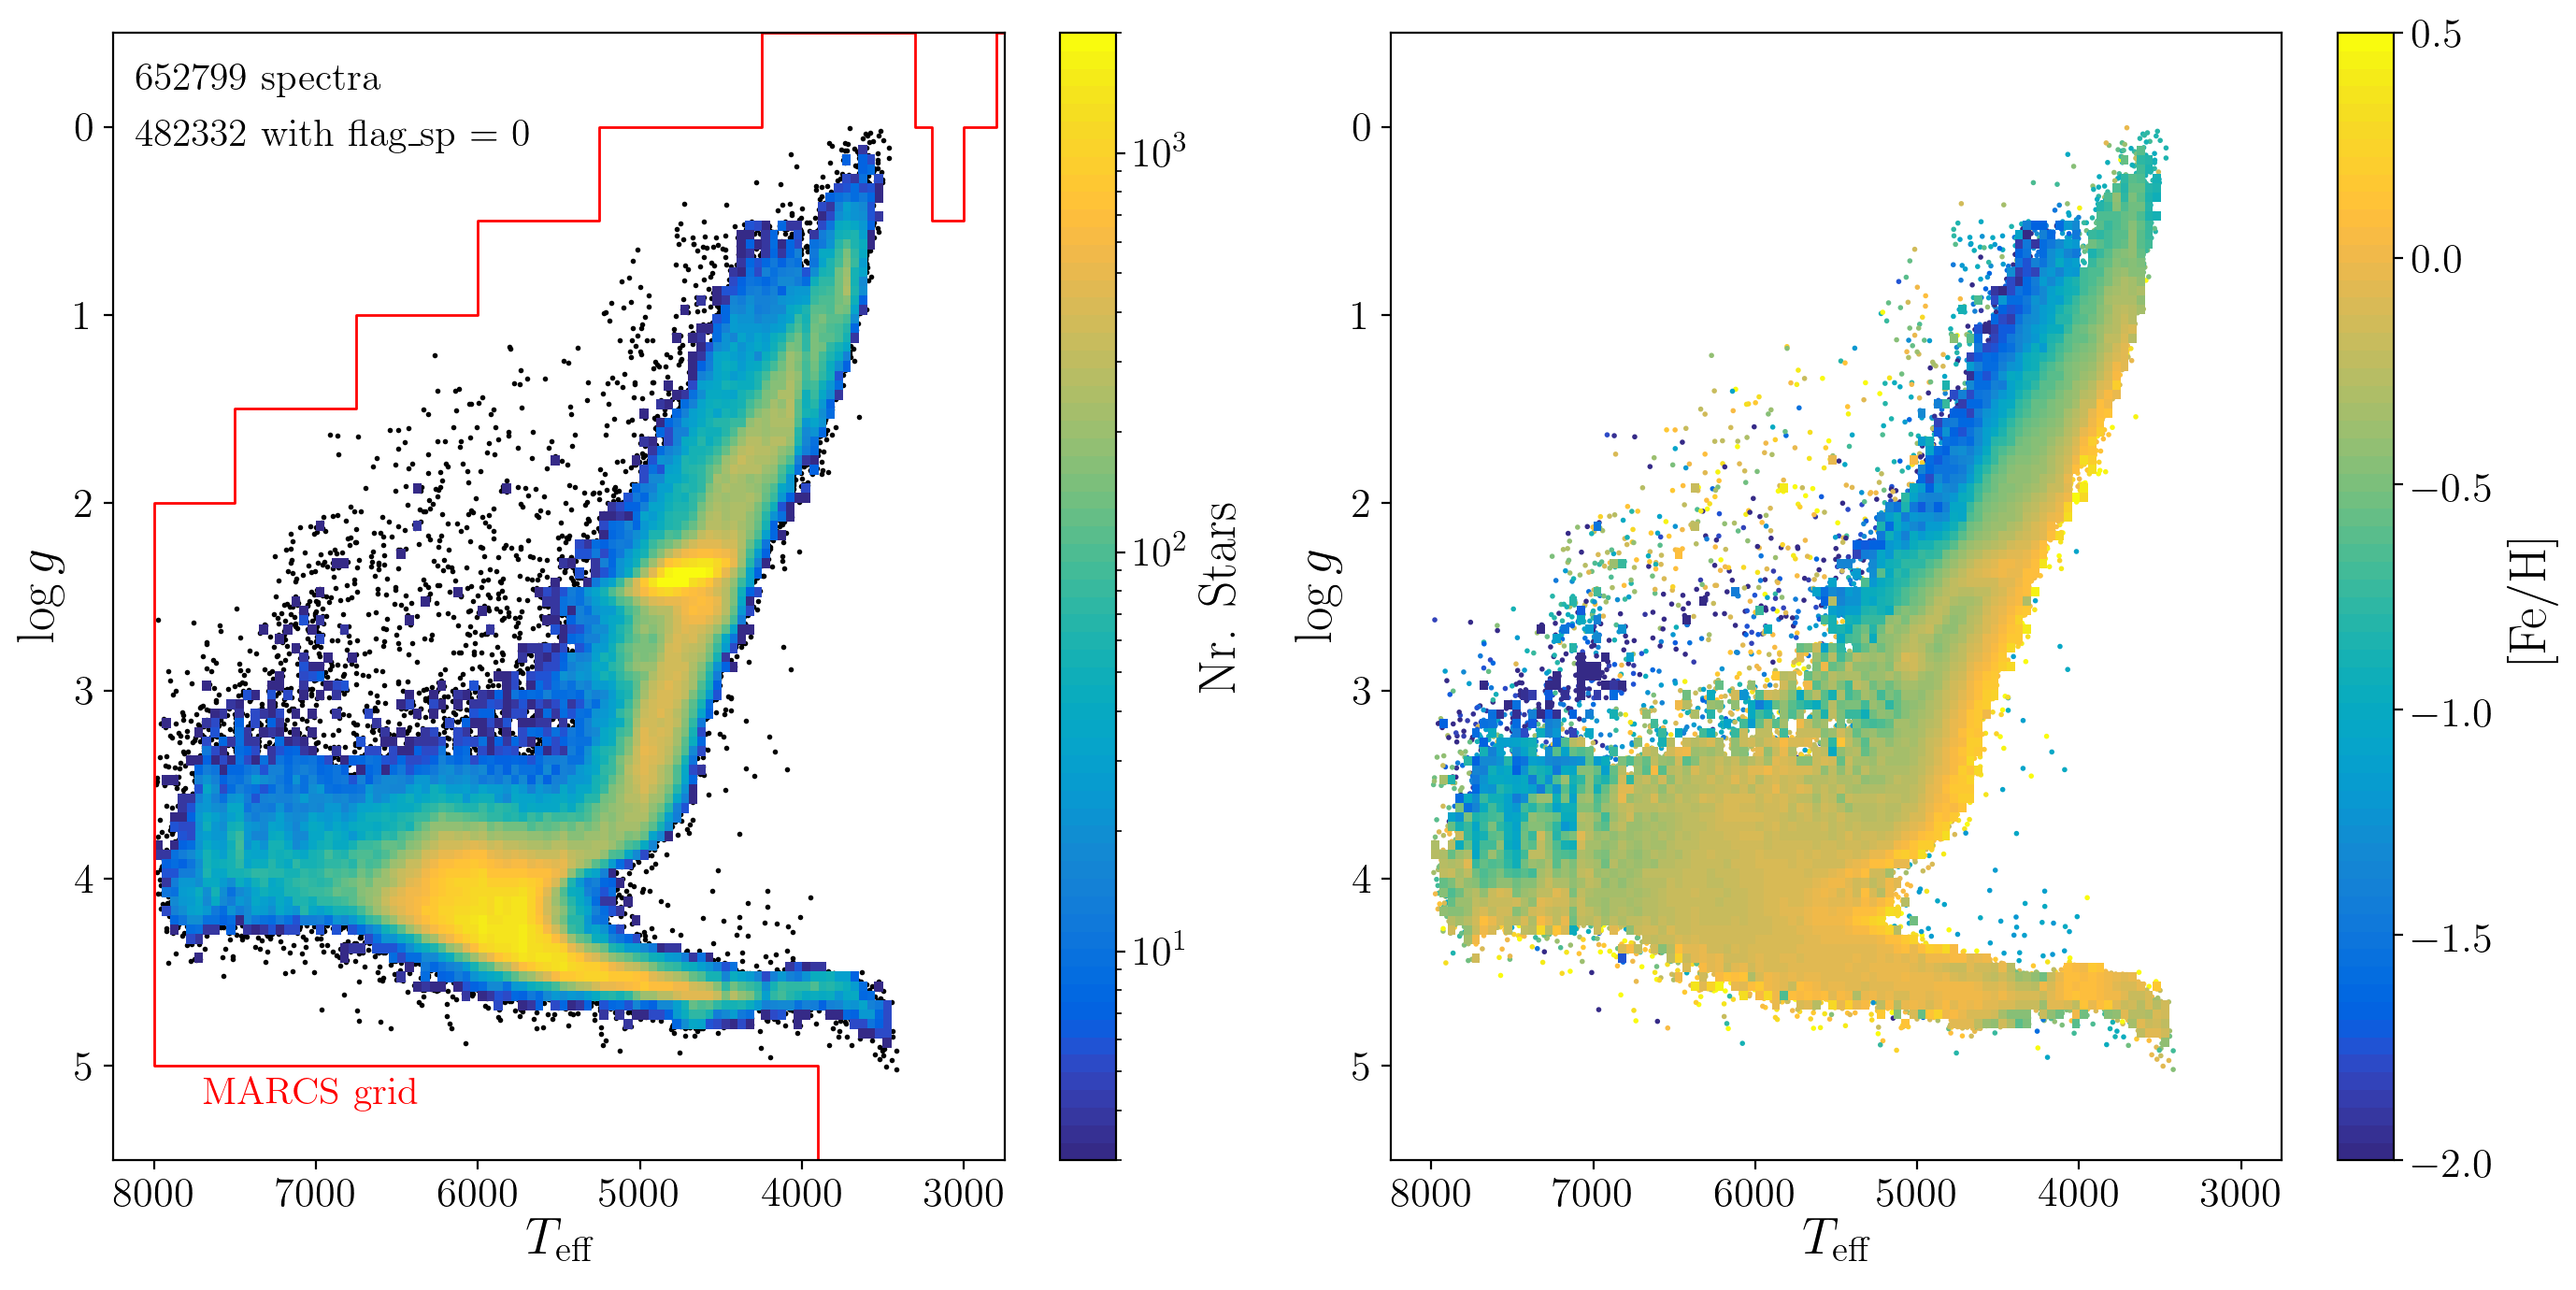
\includegraphics[width=\textwidth]{figures/Kiel_Diagram_GALAH_flag_0.png}
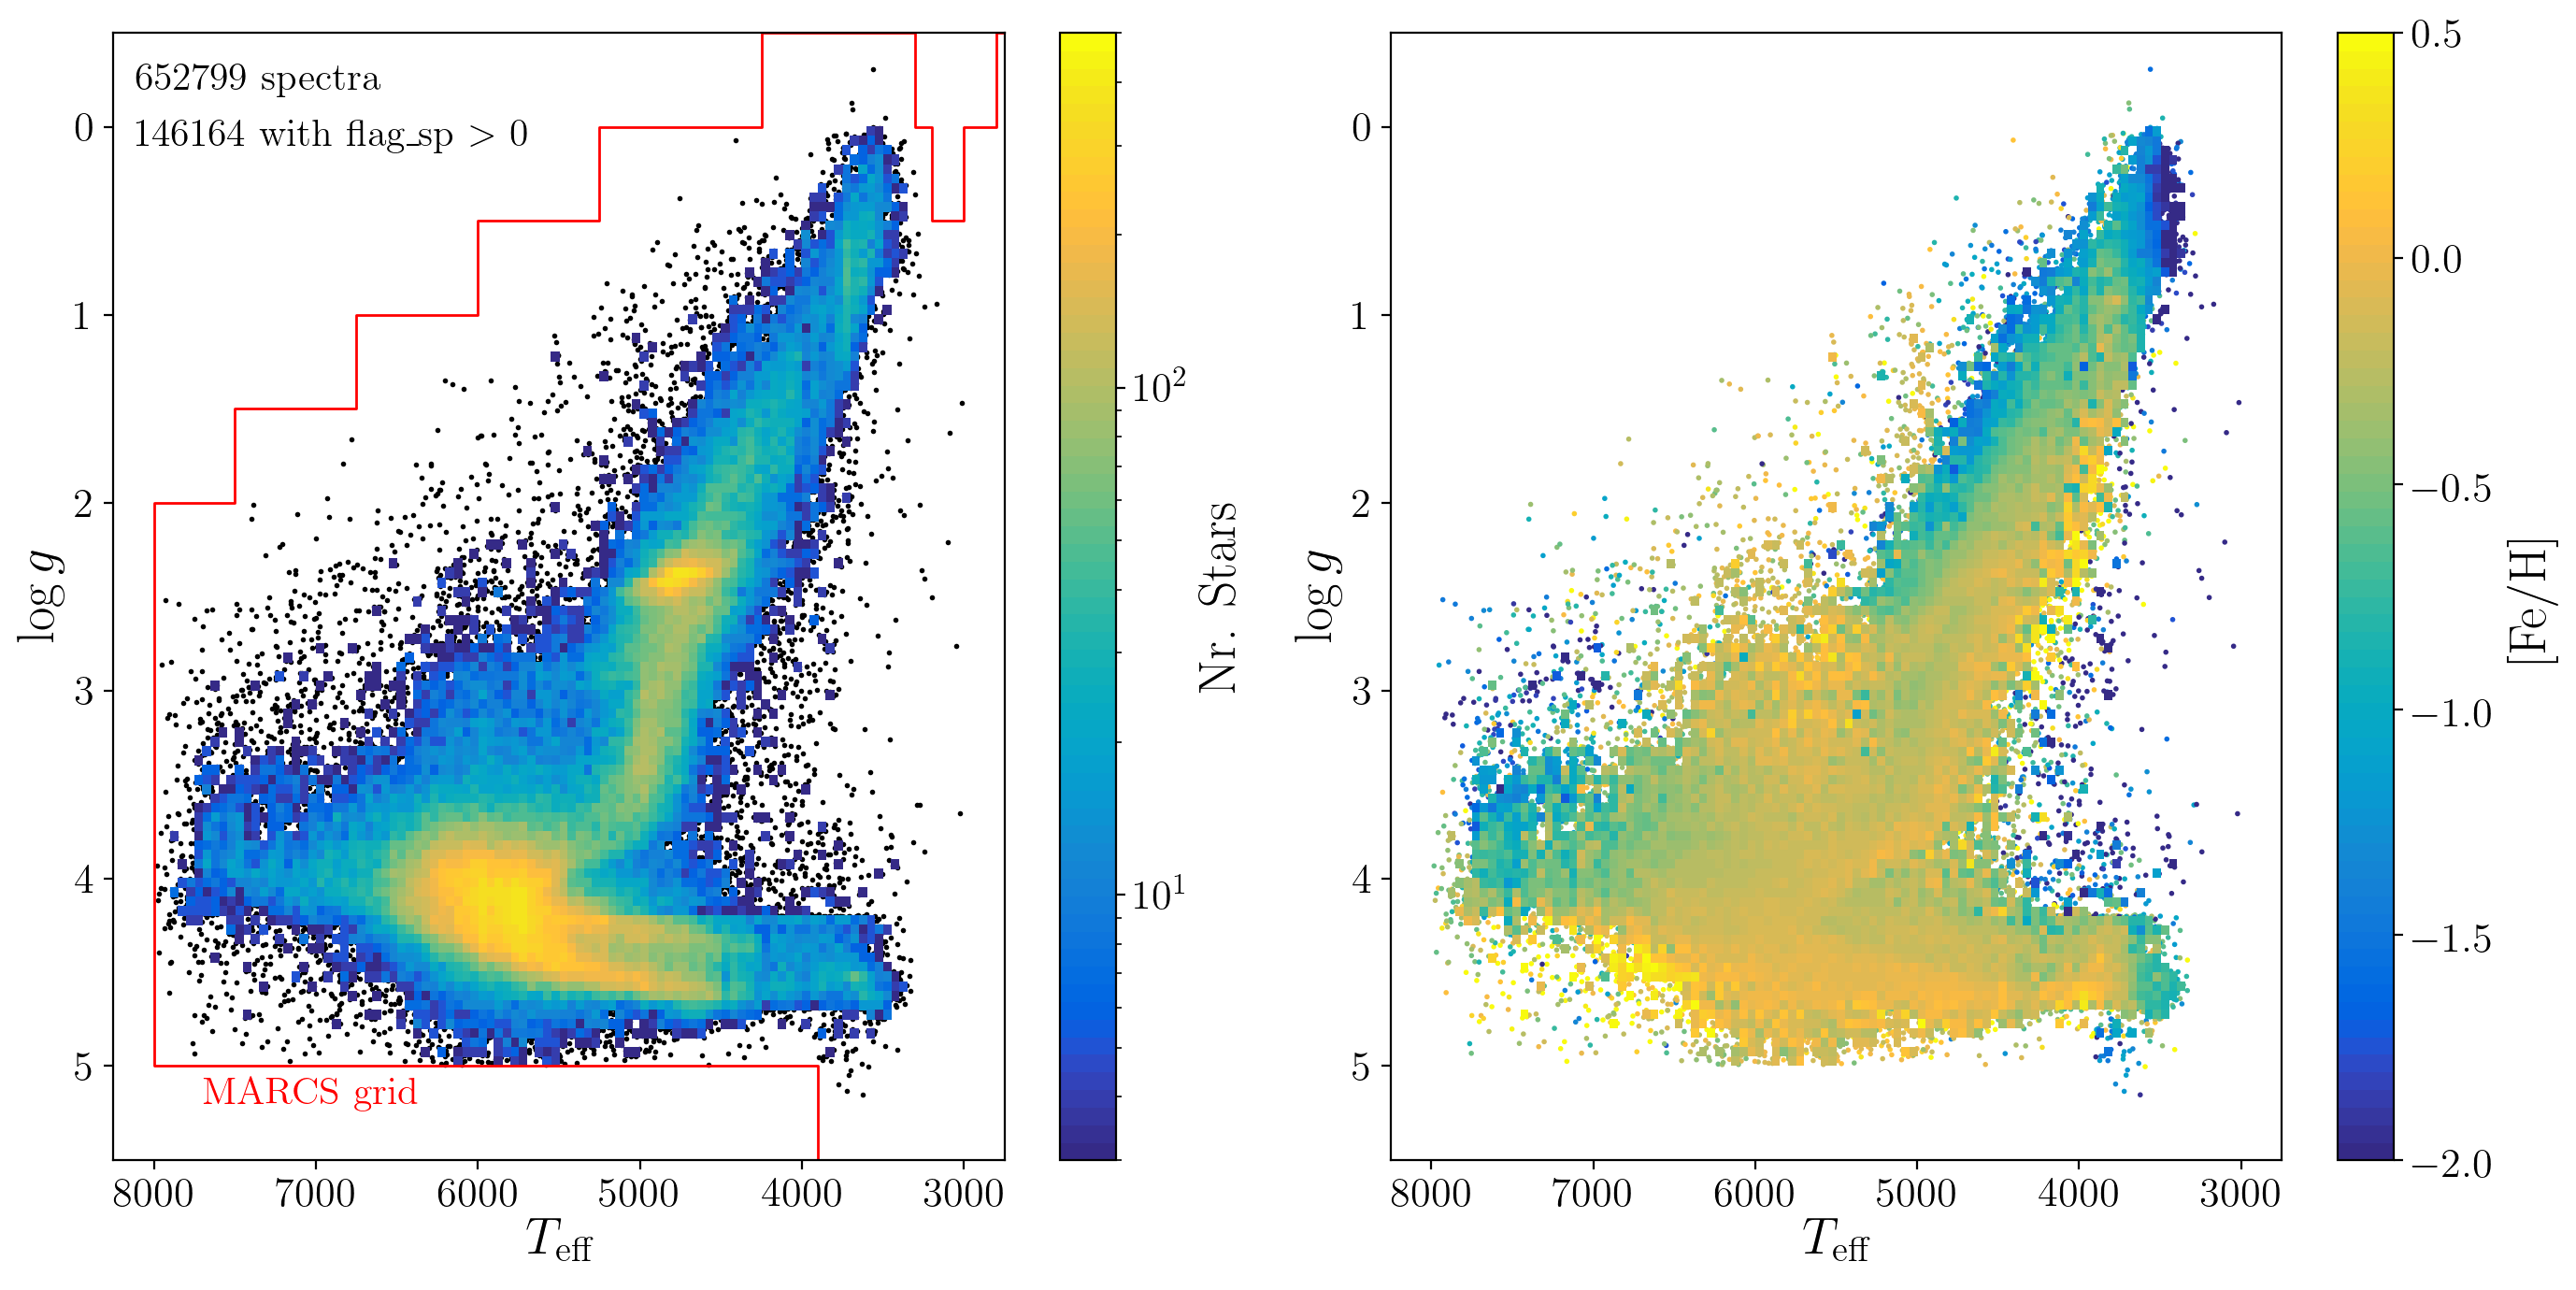
\includegraphics[width=\textwidth]{figures/Kiel_Diagram_GALAH_flag_not0.png}
\caption{Kiel diagrams ($T_\text{eff}$ vs. $\log g$) color coded by the density of stars per bin (left panel) and mean iron abundance [Fe/H] within a bin (right panel) for those stars of the GALAH data release 3 without raised stellar parameter flags (top panels) and those who have raised \texttt{flag\_sp}, but at least have estimated stellar parameters. The total number of spectra and those below the quality threshold are annotated in the upper left corner of the left panels. In the same panels, red lines indicate the grid limit of the {\sc marcs} atmosphere grid, which marks the limits of the synthesis computations.}
\label{fig:hrd_galah_dr3}
\end{figure*}

As for GALAH DR2 \citep{Buder2018}, we have applied the algorithm developed by \citet{Traven2017}, which combined the dimensionality reduction method t-SNE \citep{vanderMaaten2008} with the clustering algorithm \textsc{DBSCAN} \citep{Ester1996} to arrange similar looking spectra close to each other. With these technique we have been able to identify clusters of spectra with reduction issues, emission features, as well as clear line-splitting binaries. We have further identified possible astrometric binaries or pre-main sequence stars (\texttt{flag\_sp} = 64) by selecting the oldest {\sc parsec} isochrones for the particular iron abundance of each star and selecting all stars with surface gravity lower by $\Delta \log g = 0.15$ and cooler by $\Delta T_\text{eff} = 150\,\mathrm{K}$. This selection is most effective for the identification of binaries on the secondary main-sequence (with slightly lower $\log g$). For stars with equal bolometric luminosity, for example a binary system with the same stellar parameters, the estimated $\log g$ can be smaller by up to $\sim 0.3$. This deviation can be approximated via Eq.~\ref{eq:logg} when assuming that the bolometric luminosity of the system is twice that of a single star and the mass is estimated to be that of a single star, so that $\Delta \log g \sim - \log L_\text{bol, binary} + \log L_\text{bol, single} = - \log \left( 2 \cdot L_\text{bol, single} \right) + \log L_\text{bol, single} = - \log 2 $. We have also identified unreliable parameter estimates for the coolest bright giants, for which unreasonably low iron abundances have been estimated (see tip of the RGB in right panel of Fig.~\ref{fig:hrd_galah_dr3}).

\section{Validation of element abundances} \label{sec:validation_ab}

We validate element abundances in terms of accuracy and precision. Following this approach, we also elaborate on these two validations separately. Because we are not limited to the training set selection influence for this data release, we have also tried to estimate more upper limits and outline our approach in this section, followed by the description of our flagging algorithms with the aim to allow the community to make informed choices on the use of abundance measurements. \textbf{As for the previous data releases, we want to stress that we discourage the use of flagged element abundances without consideration of the possible systematics that these flagged measurements can introduce.}

% Should we write this here or in the WORKFLOW section?
For element abundances, we do not report uncertainties in terms of accuracy. We are aware that this leads to an underestimation of the systematic uncertainties, but want to stress that a proper estimation of the accuracy uncertainties would have to involve the systematic influence of the individual stellar parameters within their uncertainties, the uncertainties of the absolute abundances / zeropoints in terms of $\log gf$ values and additional uncertainties from the fit to the sky flat, Arcturus, the comparison with the solar circle sample, as well as the solar twin comparison. For computational reasons we have not been able to quantify all of these influences, but report them if possible (see e.g. Tab.~\ref{tab:solar_reference_values2}).

Contrary to the stellar parameters, our reported final uncertainties are thus limited to 
\begin{equation}
e_\text{final}^2 (X) = \text{max} \left(e_\text{fit}^2(X) + e_\text{repeats}^2(X) \right). \label{eq:final_error_abundances}
\end{equation}

\subsection{Accuracy of element abundances} \label{sec:accuracy_abundances}

We estimate our element abundances by changing the absolute abundance for each element that is measured in the chemical composition of the model atmosphere. We report the raw values of these measurements, A(X1234) for the $1234\,\mathrm{\AA}$ line of element X in the VAC for abundances (see Sec.~\ref{sec:value_added_catalogs}). We subtract the Solar value A(X1234), that we define for this data release (see Tab.~\ref{tab:solar_reference_values2}), from this measurement to estimate the ratio [X/H] and for element other than Fe, we further subtract the iron abundance to estimate the ratio [X/Fe].

In addition to the definition of the abundance zeropoints, we also validated the accuracy of our element abundances by comparison to measurements of the GBS, Solar twin stars as well as open and globular cluster stars.

\paragraph*{Abundance zeropoints}

Following the definition of the bracket notation, the Solar value A(X1234) should be strictly estimated from the measurement of the particular line in the Solar spectrum. For several lines of the GALAH wavelength range, however, we are facing difficulties to estimate the solar A(X1234). Firstly, via 2df-HERMES, we can only perform sky (flat) observations rather than observing the Sun directly. Secondly our observation setup is not the same as for the normal setup of our observations. Thirdly, some lines are either not detectable (even within high $S/N$ spectra) or their equivalent width or line strength does not increase significantly with increasing A(X), that is, we perform a measurement at a plateau on the curve of growth. Contrary to many other studies or surveys, we do decide to also report the absolute abundances and only use laboratory oscillator strengths ($\log gf$) rather than tuning these astro-physically based on the solar spectrum with literature abundances. There are thus several solutions available to still estimate abundance zeropoints, which we will discuss subsequently:
\begin{enumerate}
\item Measure A(X) from same line in Solar / sky flat / asteroid spectrum.
\item Use a different line in solar spectrum (because A(X) has to be the same).
\item Use another benchmark star (like Arcturus) via bridge measurements. For this one would measure the line that is weak in the Sun in Arcturus as well as another line of the element that is strong enough in both stars. In that case the difference in A(X) for the lines in Arcturus can be used to transfer them onto lines in the Sun.
\item Use the element abundance ratios of stars in the solar circle, for studies suggest that the abundances should be Solar. APOGEE follows this approach to estimate their zeropoints since their DR14 \citep[see][]{Holtzman2018, SDSSDR16}.
\item Compare with a literature study, e.g. via the estimates for Arcturus \citep[e.g.][]{Ramirez2011}, Solar twins \citep[e.g.][]{Bedell2018} or the overlap with a different survey, e.g. APOGEE DR16 \citep{SDSSDR16}.
\end{enumerate}

For GALAH DR3 we try to use the first method whenever possible and validate it with the other approaches. Whenever this approach was not useable or the differences to the other methods were to significant (pointing to issues in the sky flat spectrum), we used the fourth and fifth option to ensure best overall consistency. \SB{Should we list here when which approach was used? That should however be rather obvious from the fact that we used it if the skyflat [X/Fe] is not $0.00\,\mathrm{dex}$...}

% Based on the outcome of GALAH_DR3/validation/abundances/solar_abundance_analysis.ipynb
% The adopted abundance zeropoints are listed in Table tables/solar_references2.tex with \label{tab:solar_reference_values2}
Ultimately, we have decided to adopt the zeropoints for the lines and elements that are stated in Table~\ref{tab:solar_reference_values2}. For convenience we also list the values estimated by \cite{Asplund2009} to allow to identify lines with possibly wrong $\log gf$ values. We also list the results for a sky flat of GALAH DR3 (\SB{Currently 150405000901378 rather than the combined super sky flat}) as well as the average abundances for stars in the solar circle with near-solar iron abundances\footnote{We select these stars via $-0.1 < \texttt{fe\_h} < 0.1$, $\texttt{r\_est} < 500$, $\texttt{snr\_c2\_iraf} > 40$, $\texttt{flag\_cannon} = 0$, $4500 < \texttt{teff} < 6500$, and for abundances of element X additionally $\texttt{flag\_X\_fe} = 0$.}. Because we expect that this data release will be used in combination with APOGEE DR16 to explore the Galaxy, we also list the values from APOGEE DR16 for the asteroid VESTA as well as the differences of the overlapping observations\footnote{We have used all x-matches, including repeats, via 2MASS IDs and then further restricted the overlap sample to stars with $\texttt{flag\_sp} = 0$, $\texttt{snr\_c2\_iraf} > 100$, $\texttt{ASPCAPFLAG} = 0$, $\texttt{SNR} > 100$, and for abundances additionally to reasonable, finite measurements ($\mathrm{[X/Fe]} > -5\,\mathrm{dex}$) of unflagged elements with $\texttt{flag\_X\_fe} = 0$ and $\texttt{X\_FE\_FLAG} = 0$.} of GALAH DR3 and APOGEE DR16.

We want to stress, that more work is needed to scrutinise the line selection and abundance zeropoints further. Due to time and computation restrictions during the implementation of the new NLTE grids, we have only been able to run these elements combined, rather than line-by-line. However, the line-by-line analysis of element abundances has been shown to been important for several elements (e.g. Al, Ca, and Ba) and has to be done in future releases to improve the accuracy and precision of abundance measurements further.

\paragraph*{Abundances of Arcturus and other GBS stars}

\SB{This comparison is not vital, but I want to include it, because we can use it to assess what we can do for the highest $S/N$ spectra. The GBS values in this case are not external, but this time also underly the influences from the analysis methods and the limitations of the FLAMES/UVES spectra.}
Arcturus: Analysed in detail by \citet{Ramirez2011} and used by APOGEE as reference object. For comparison, we list the values for Arcturus in Table~\ref{tab:arcturus_reference_values}.

Other GBS: Fig~\ref{fig:gbs_performance_abundances}

\SB{To be continued...}
% Based on the outcome of GALAH_DR3/validation/abundances/gaia_fgk_benchmark_stars/gbs_performance_abundances.ipynb
\begin{figure*}
\centering
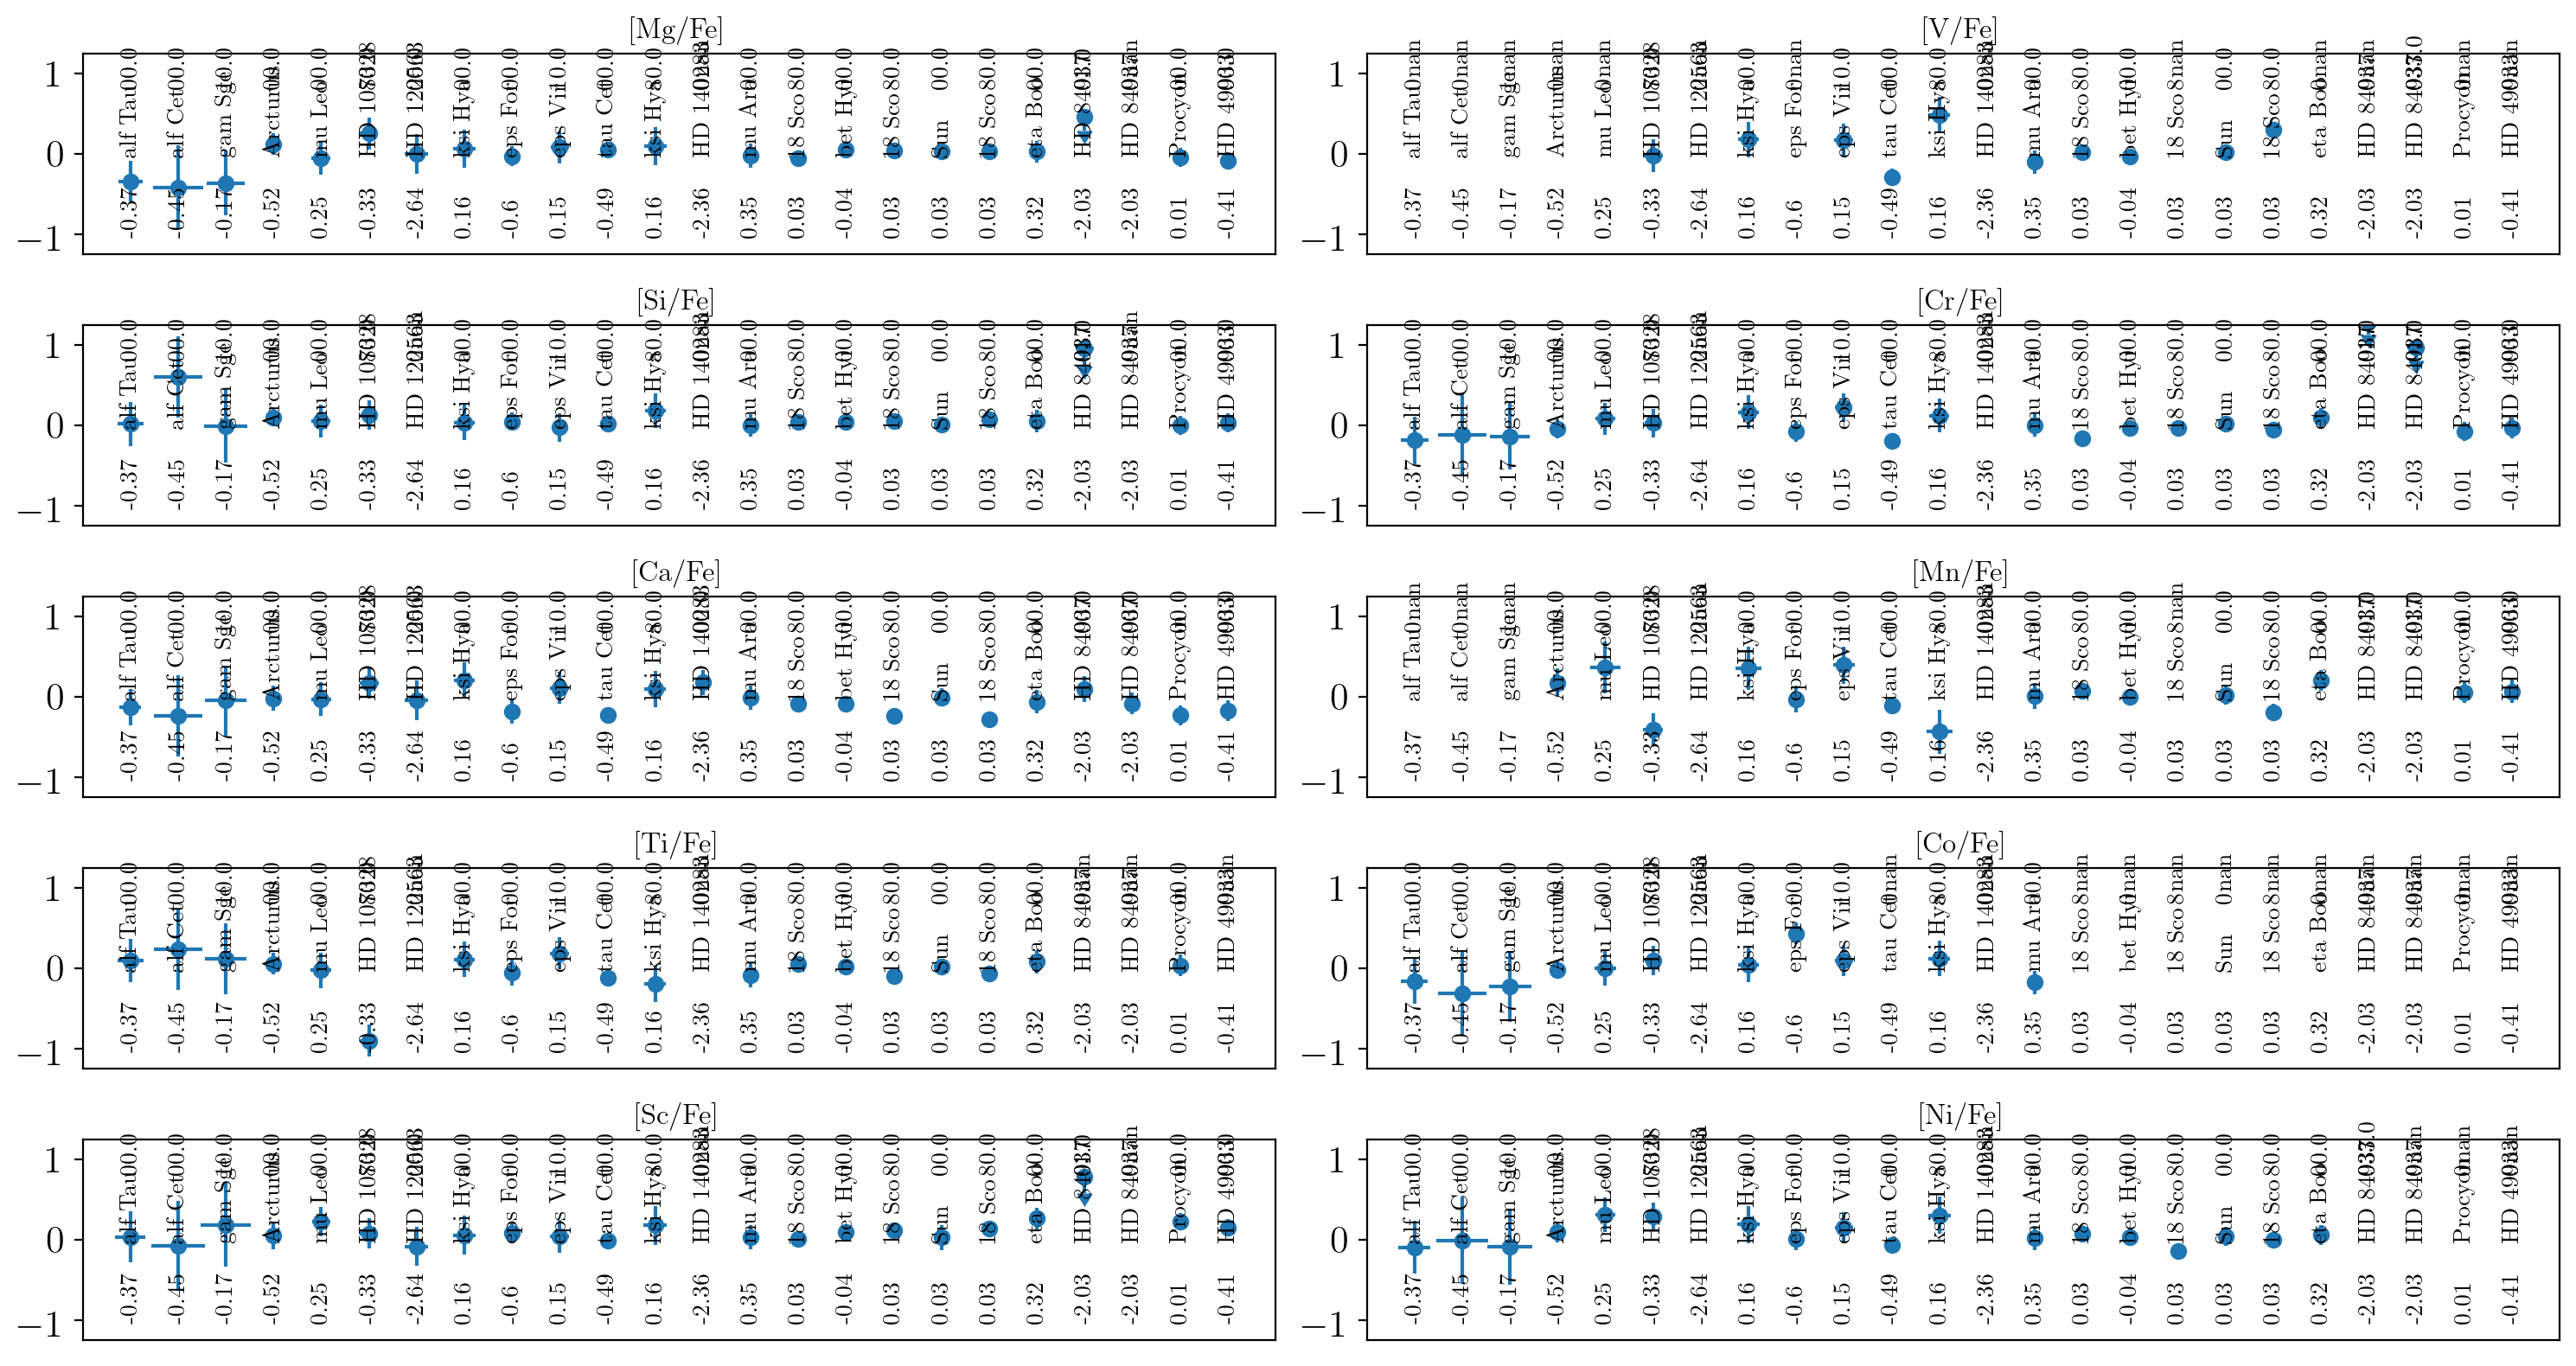
\includegraphics[width=\textwidth]{figures/gbs_performance_abundances.png}
\caption{Comparison of A(X) for the Gaia FGK benchmark stars \citep{Jofre2018a} including Arcturus. Differences are plotted as GALAH DR3 - literature. We can plot A(Mg), A(Si), A(Ca), A(Ti), A(Sc), A(V), A(Cr), A(Mn), A(Co), A(Ni). We can also plot these relative, i.e. [X/H] or [X/Fe]. Include \citet{Ramirez2011} as well.}
\label{fig:gbs_performance_abundances}
\end{figure*}

\paragraph*{Abundances of the Solar twins}

We compare the abundances of solar twins in the solar neighborhood in Fig.~\ref{fig:solar_twin_comparison} with the results from the studies performed by \citet{Spina2016} and \citet{Bedell2018}. We follow the definition of these studies and select high-quality solar twin abundances with the selection of $\Delta T_\text{eff} < 100\,\mathrm{K}$, $\Delta \log g < 0.1\,\mathrm{dex}$, and $\Delta \mathrm{[Fe/H]} < 0.1\,\mathrm{dex}$ with respect to the Solar listed in Tab.~\ref{tab:solar_reference_values1}.
For such stars, these and other studies \citep[e.g.][]{Nissen2015} have found tight correlations with abundances and stellar ages, that is, chemical clocks. Given that these studies have been performed with significantly higher $S/N$ and resolution, they are useful indicators to assess our abundance zeropoints, if we assume that firstly their found relations apply to our selection (typically further away than their sample) and secondly our age estimates agree on average with theirs. \SB{Because we use the outcome of the DR3 analysis pipeline, we decided to shift the age scale by the difference of our Solar and and the one reported by \cite{Bonanno2002}, that lower it by $1.26\,\mathrm{Gyr}$.} We plot the age-abundances distribution of the Solar twins from GALAH DR3 in Fig.~\ref{fig:solar_twin_comparison} together with the fitted relations from \citet{Bedell2018} and state the mean difference between these curves and our data for each panel. \SB{Comment on what we see: Good agreement for O, Na, Na, Si, Ca, Sc, Ti, Ti2, Mn, Zn, Y, Ba. Ok for Mg, Cr, Ni, Cu. Can not say much for C and V.}

\SB{How much does Klemen want to do this as a separate paper?}

% Based on the outcome of GALAH_DR3/validation/comparisons/comparison_solar_twins/solar_twin_comparisons.ipynb
\begin{figure*}
\centering
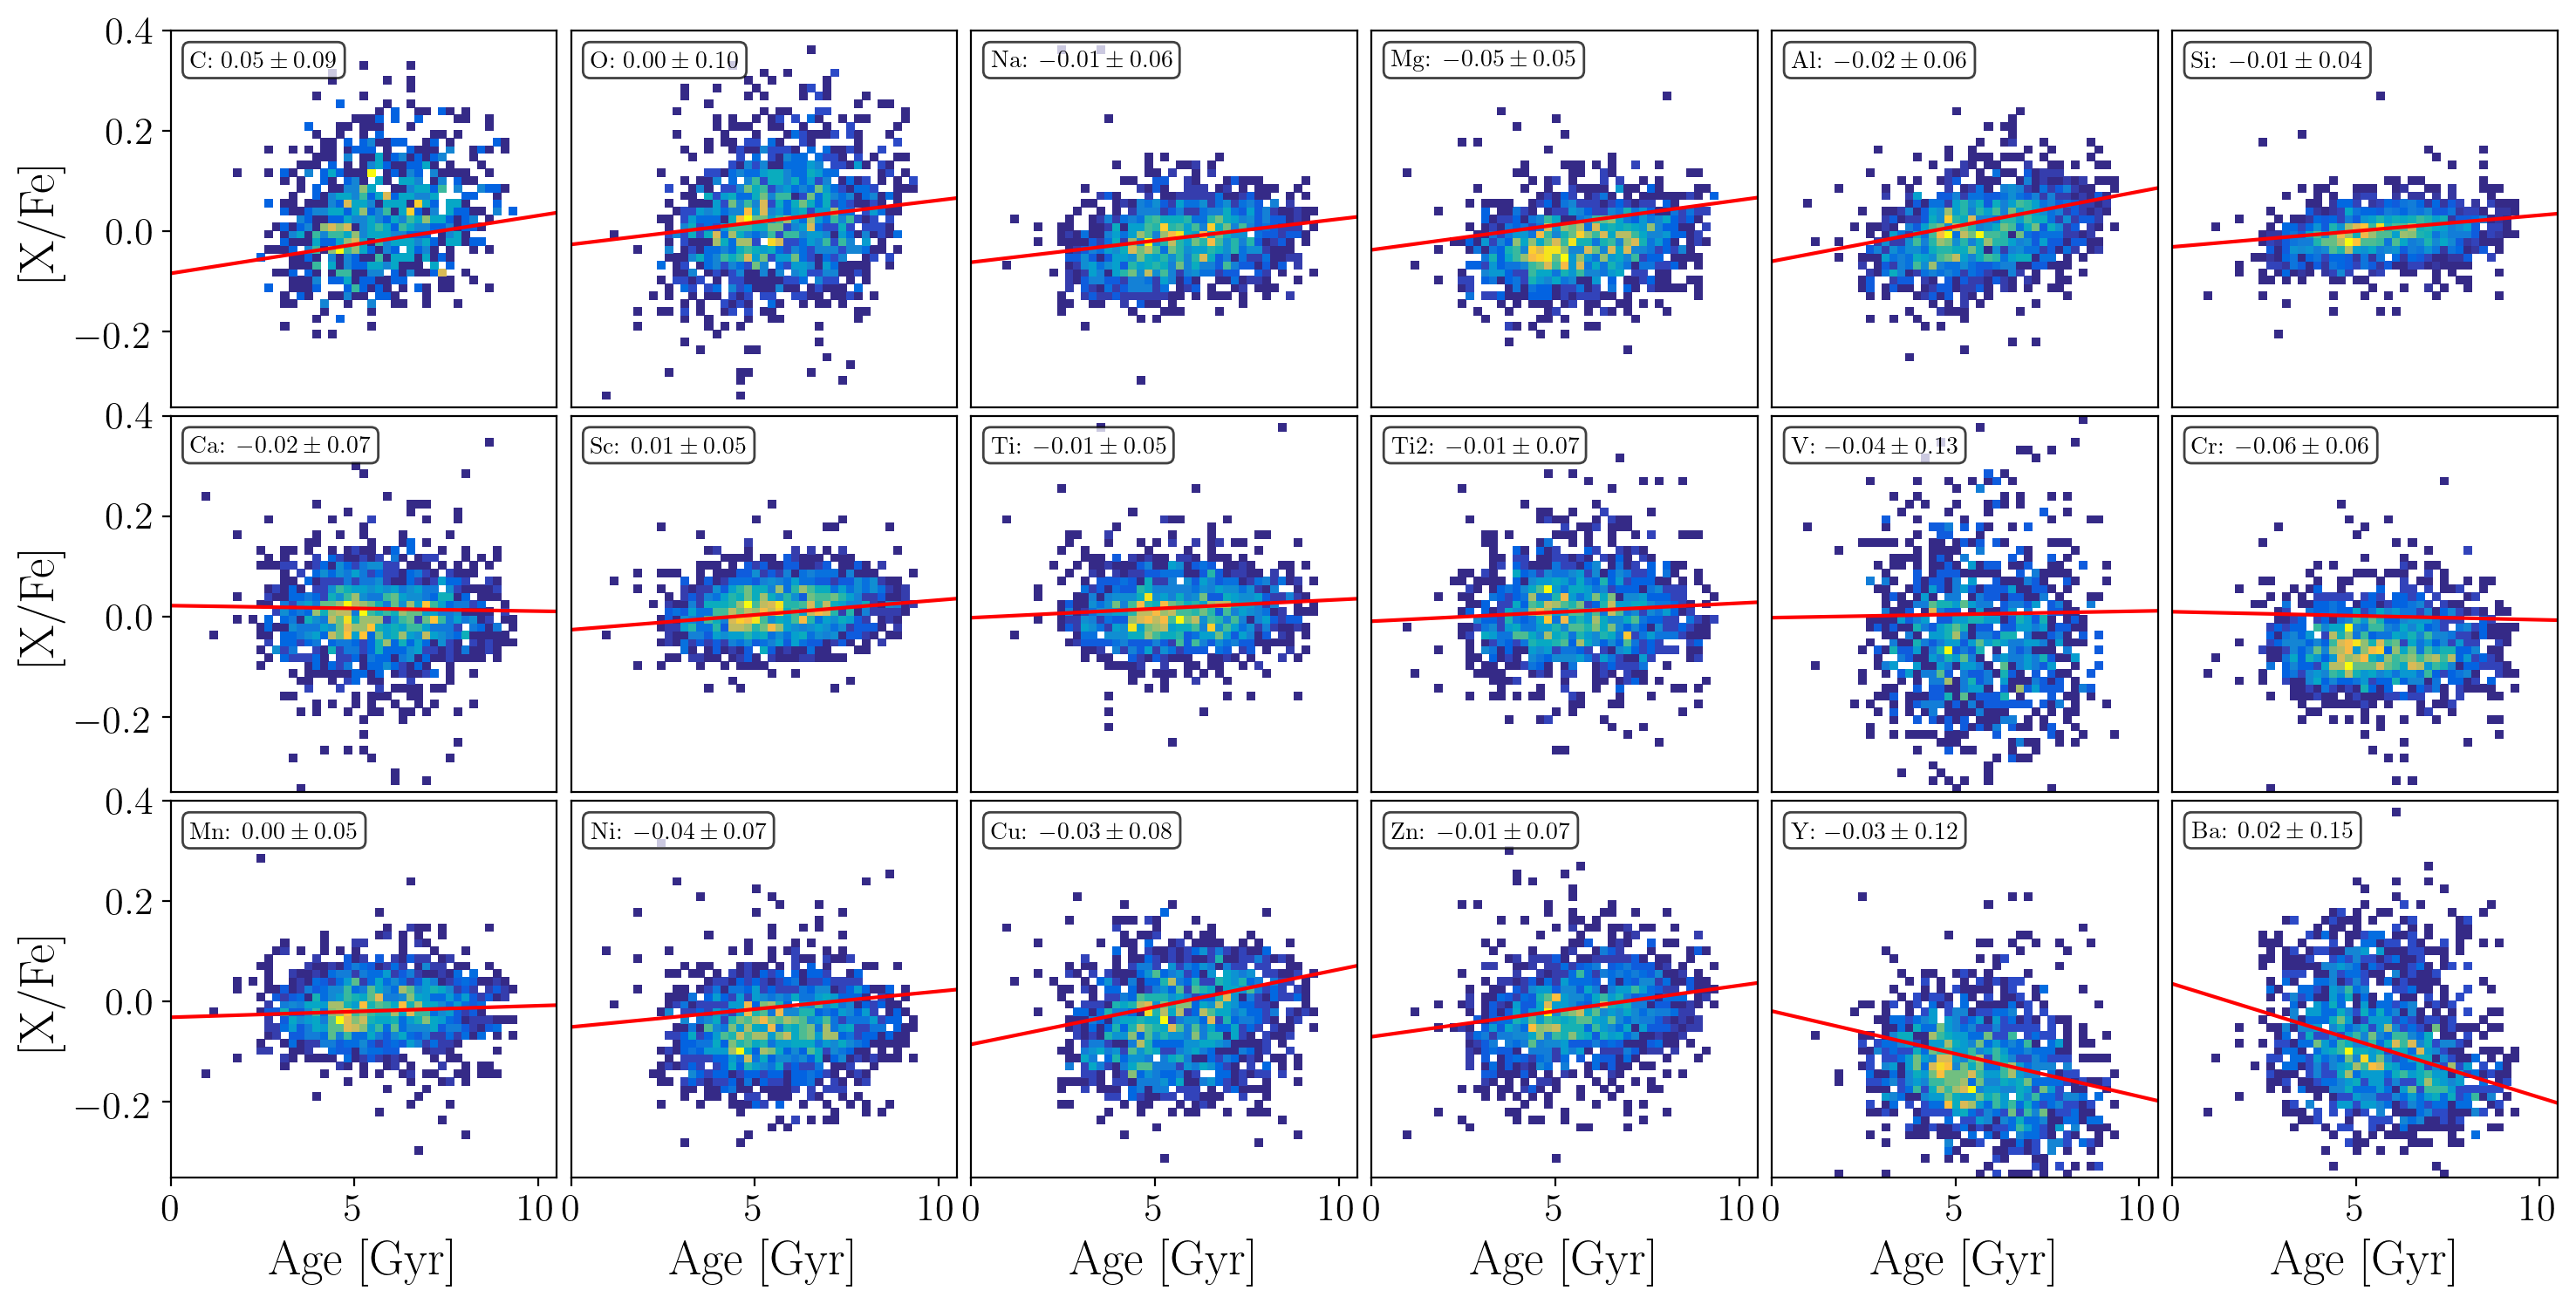
\includegraphics[width=\textwidth]{figures/solar_twin_comparison.png}
\caption{Chemical abundances $\mathrm{[X/Fe]}$ as a function of age \SB{(currently from the DR3 analysis pipeline shifted by $-1,26\,\mathrm{Gyr}$ - should we plot BSTEP?)} for solar twins. We over plot in red the functions calculated by \citet{Spina2016, Bedell2018}.}
\label{fig:solar_twin_comparison}
\end{figure*}

\paragraph*{Abundances of the cluster stars}

\SB{Here we should at least talk about some interesting abundance correlations! Especially the Na-O and Mg-Al anticorrelations. Also look at the neutron-capture elements and include plots for atomic diffusion (which we would do anyway because we plot [X/Fe] vs. Teff and logg!}

Na-O anticorrelations \citep{Carretta2009}
Intrinsic GC metallicity spread \citep{Carretta2009b}

\DN{I think it would be good to also include a comparison with 47 Tuc, which is well-sampled by GALAH, as that will enable you to evaluate GALAH's precision in the low-metallicity regime. See David Nataf's email from 200402 on the 47 Tuc selection and isochrone choice to overplot.}

David Yong: Ba-rich star in 47Tuc: \citep{Cordero2015} \\
n-process anticorrelations: \citep{DOrazi2010}


% Created with GALAH_DR3/validation/comparisons/comparison_clusters/GALAH_DR3_Comparison_Clusters.ipynb
\begin{figure*}
\centering
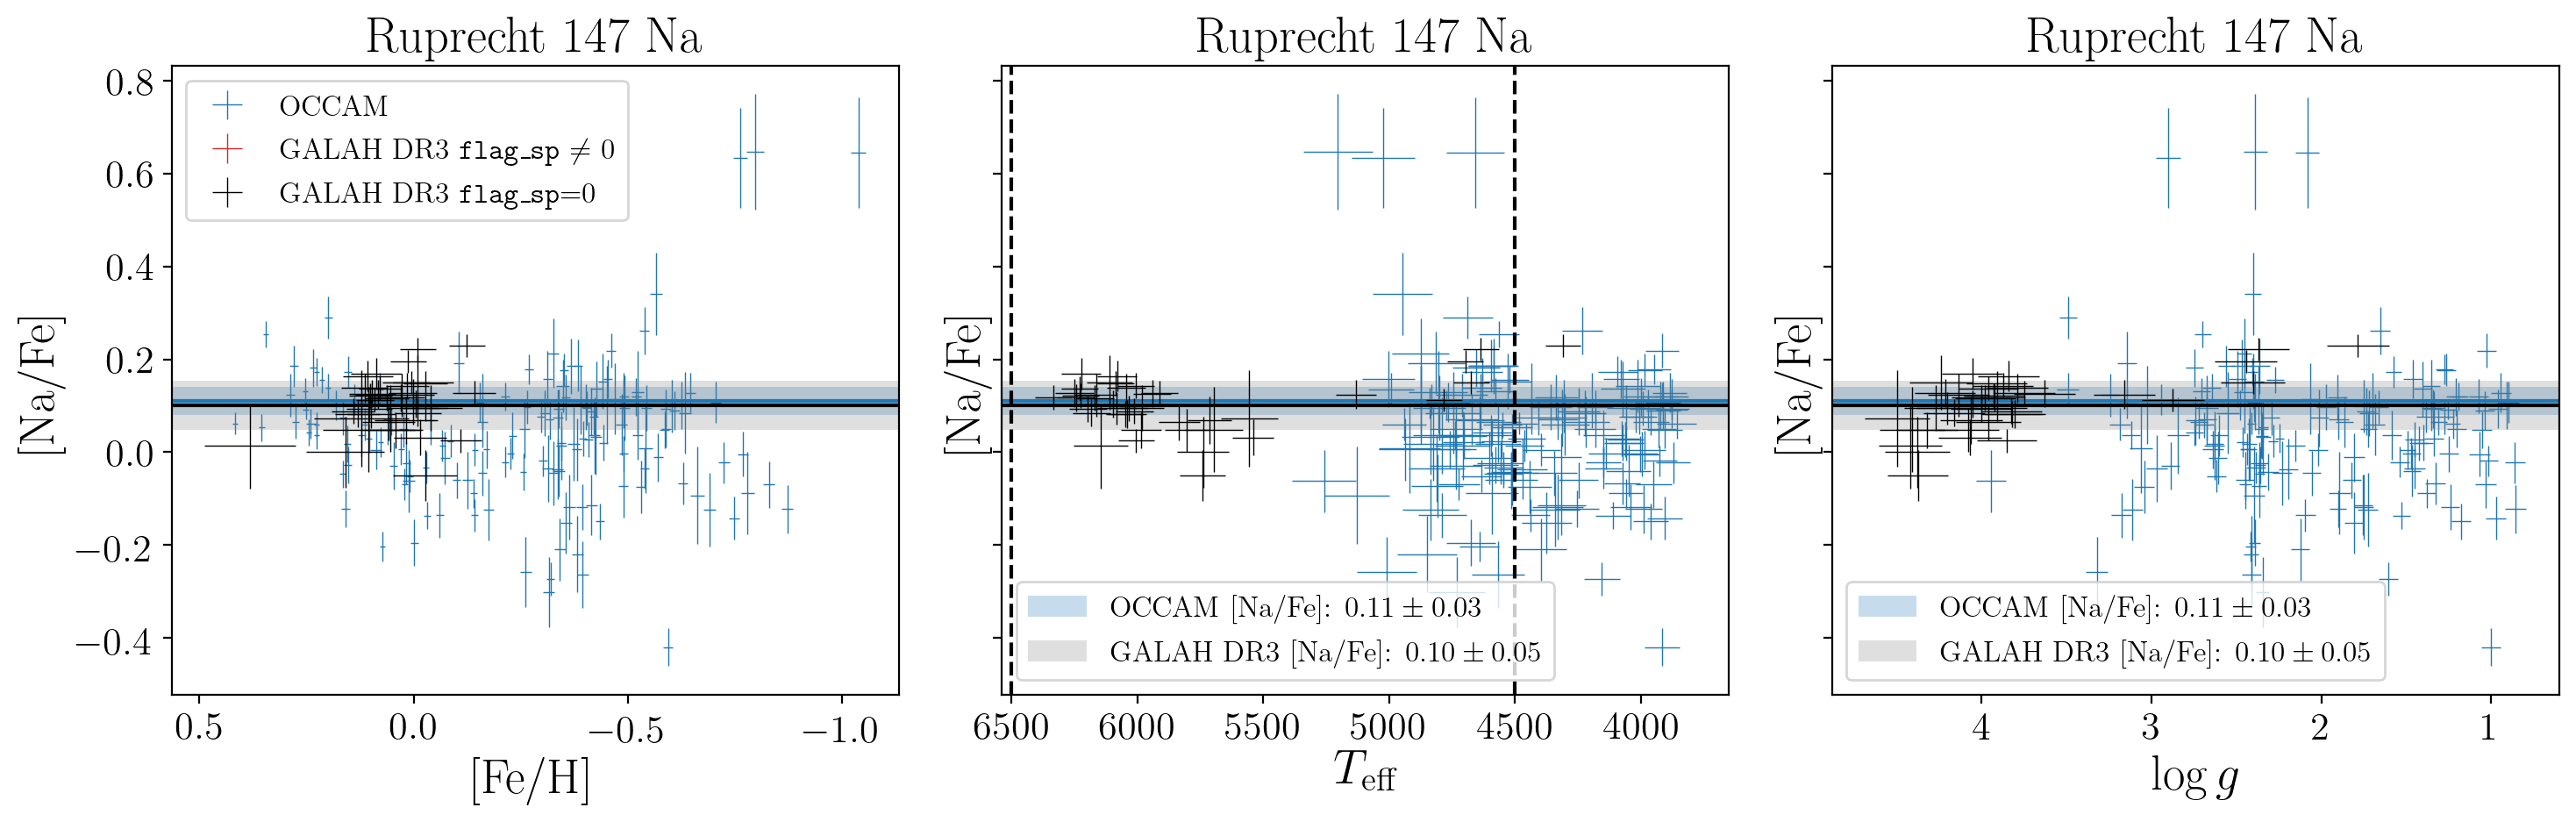
\includegraphics[width=0.49\textwidth]{figures/oc_Na_Ruprecht_147.png}
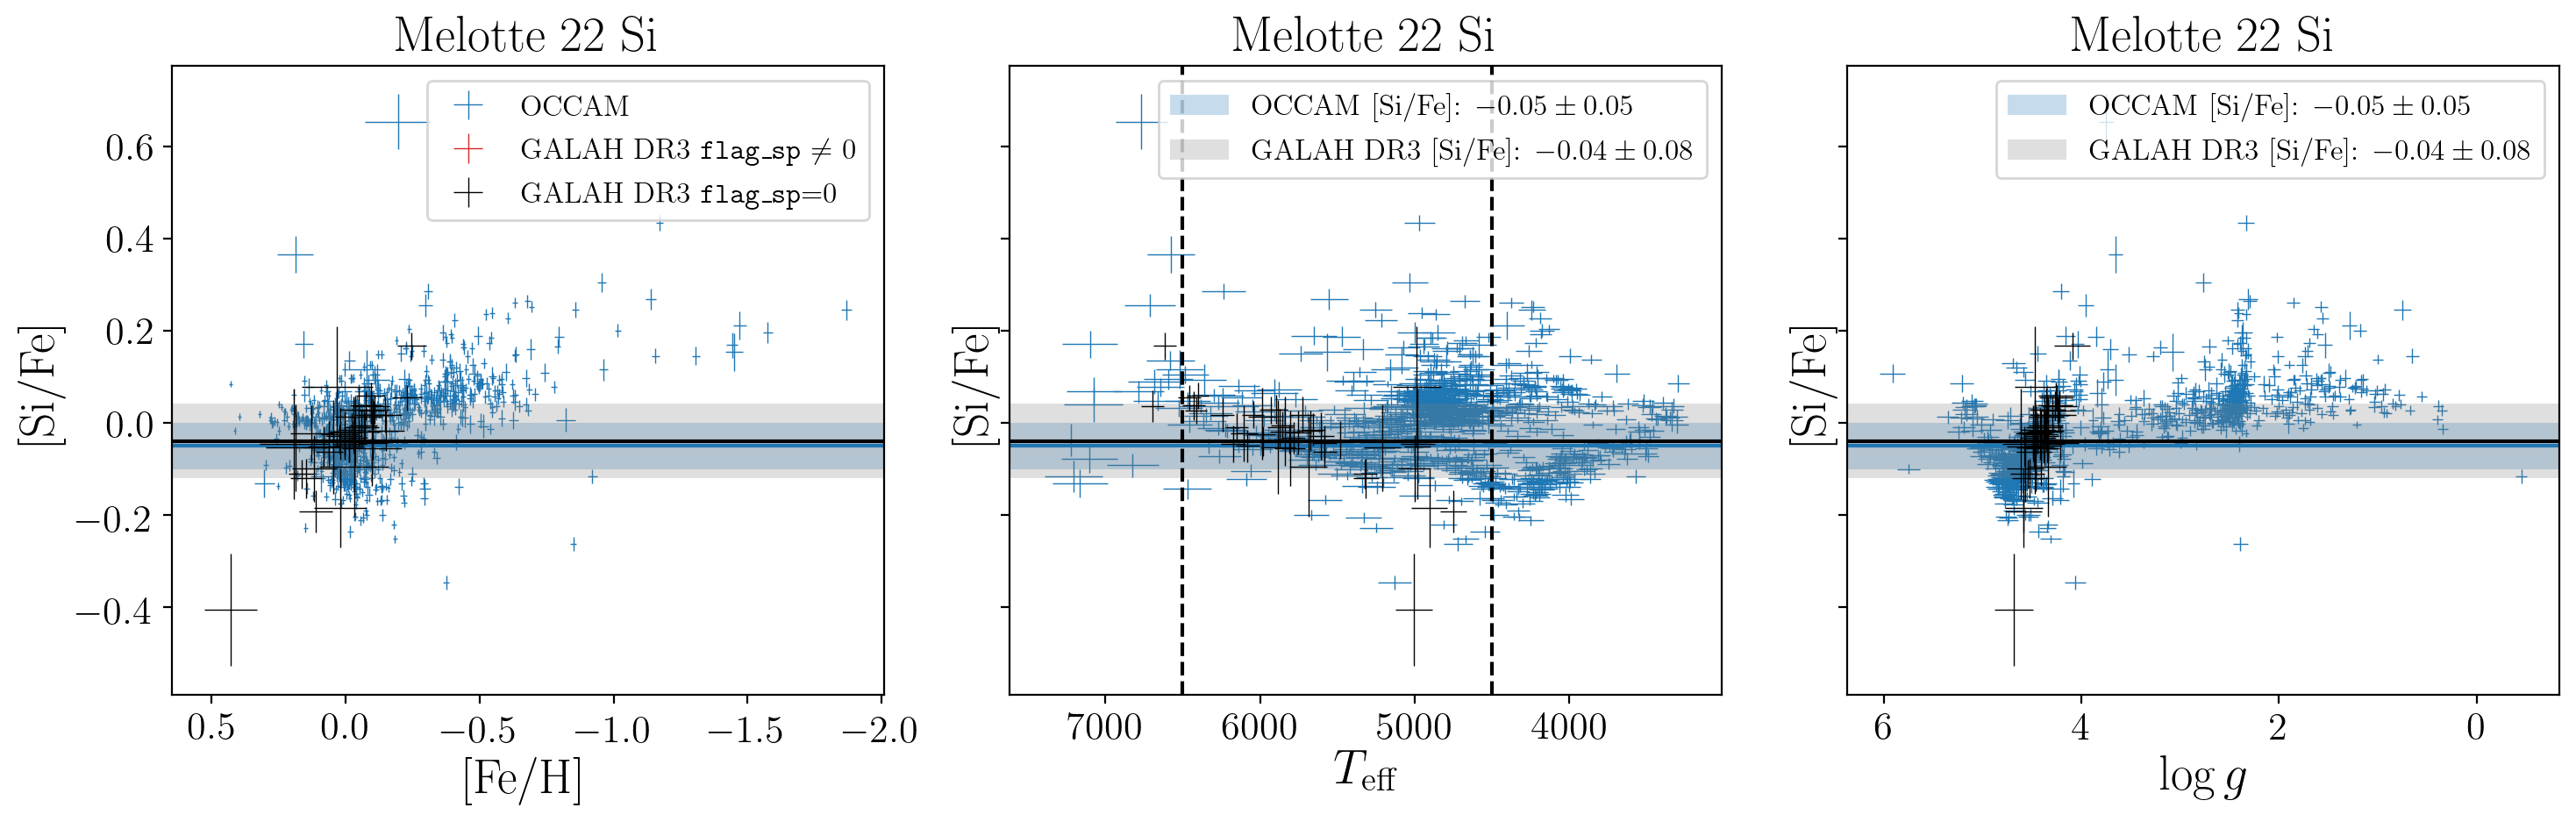
\includegraphics[width=0.49\textwidth]{figures/oc_Si_Melotte_22.png}
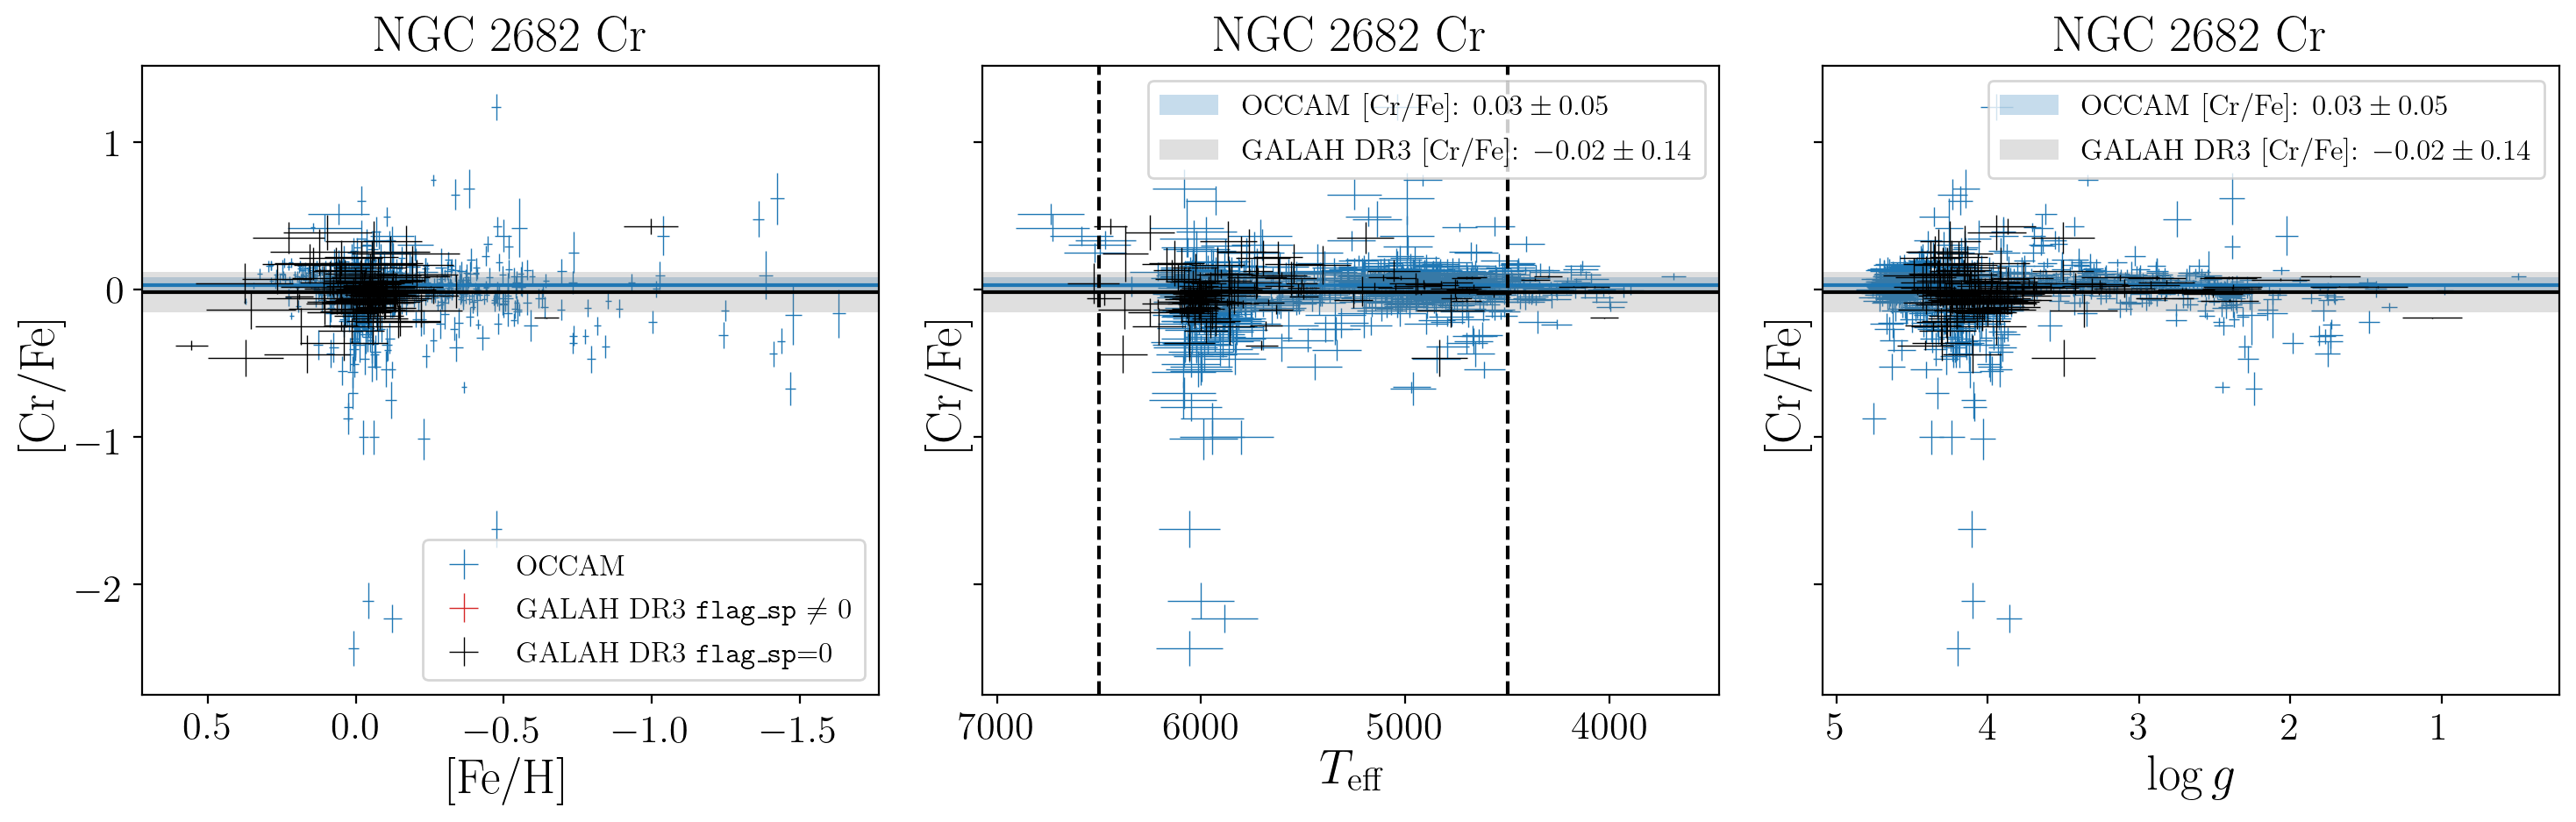
\includegraphics[width=0.49\textwidth]{figures/oc_Cr_NGC_2682.png}
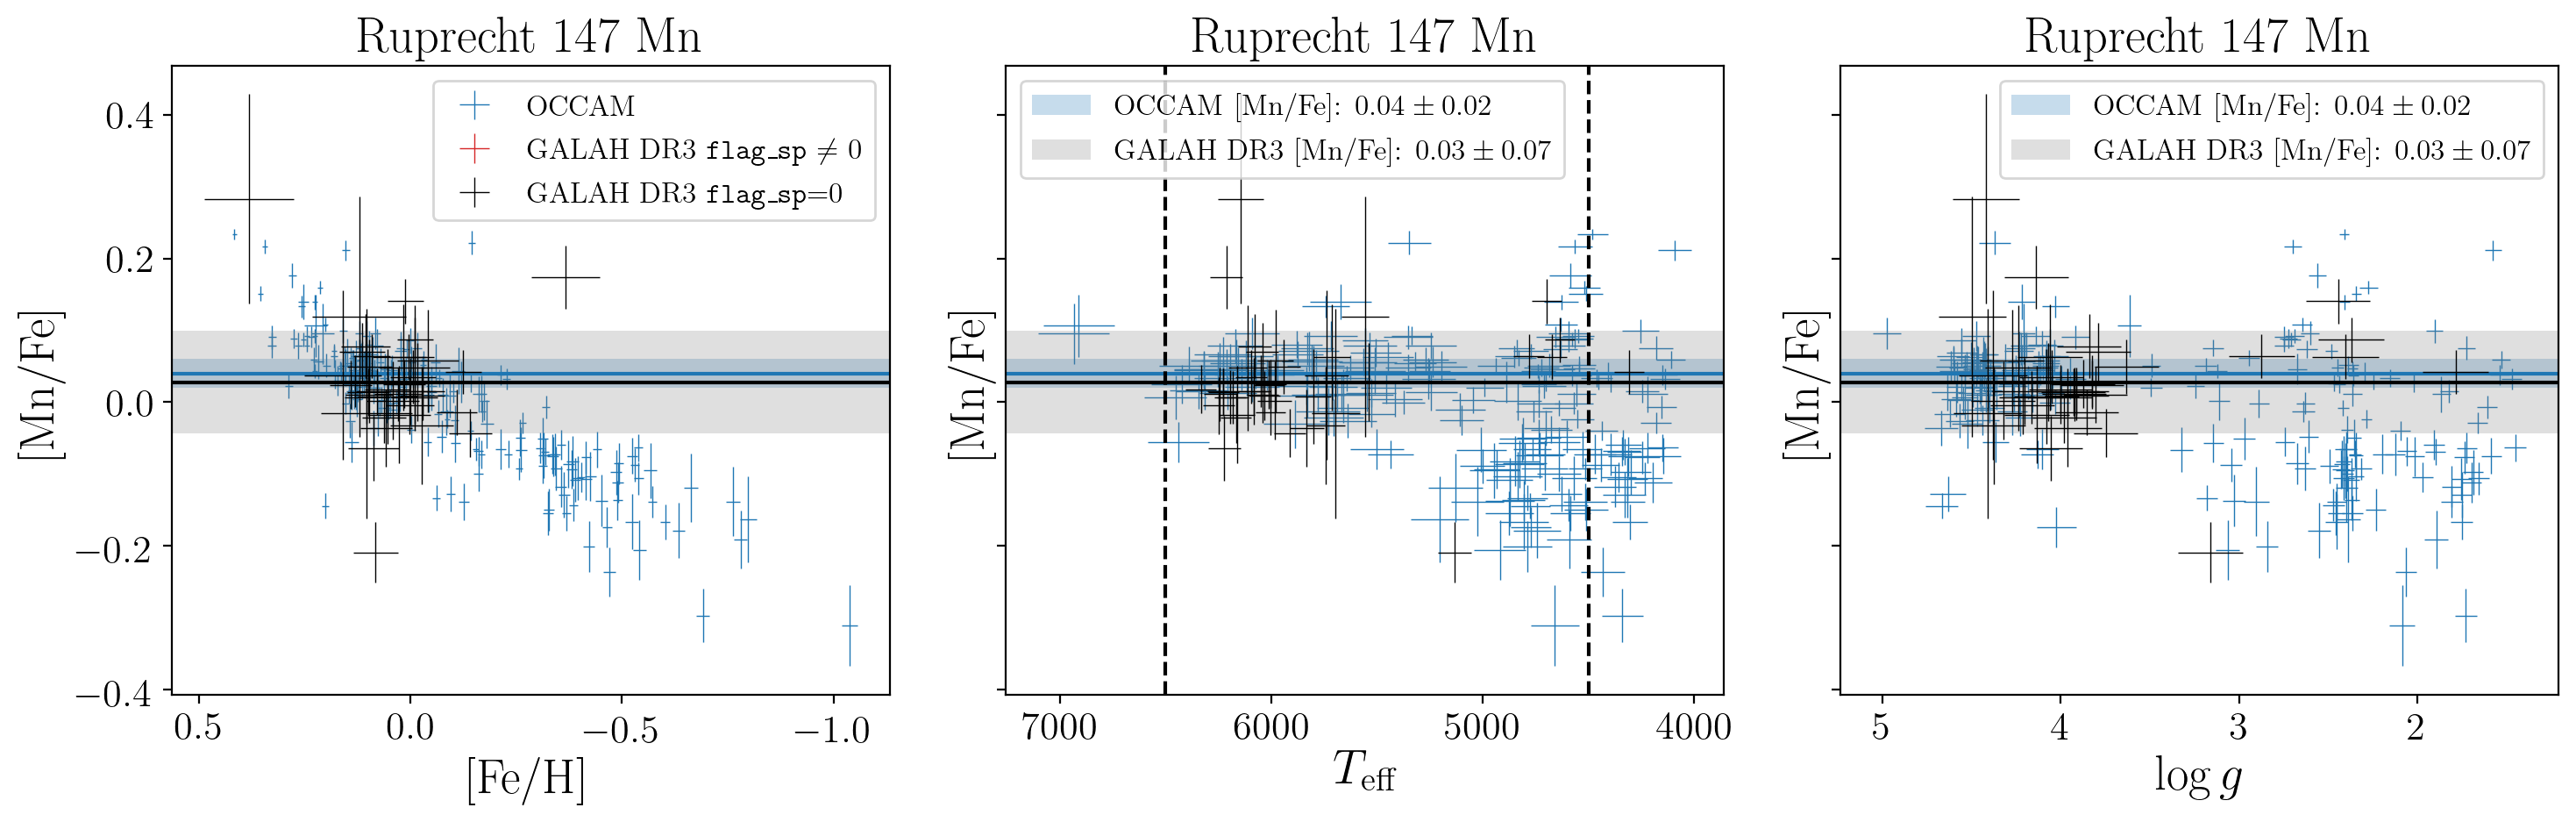
\includegraphics[width=0.49\textwidth]{figures/oc_Mn_Ruprecht_147.png}
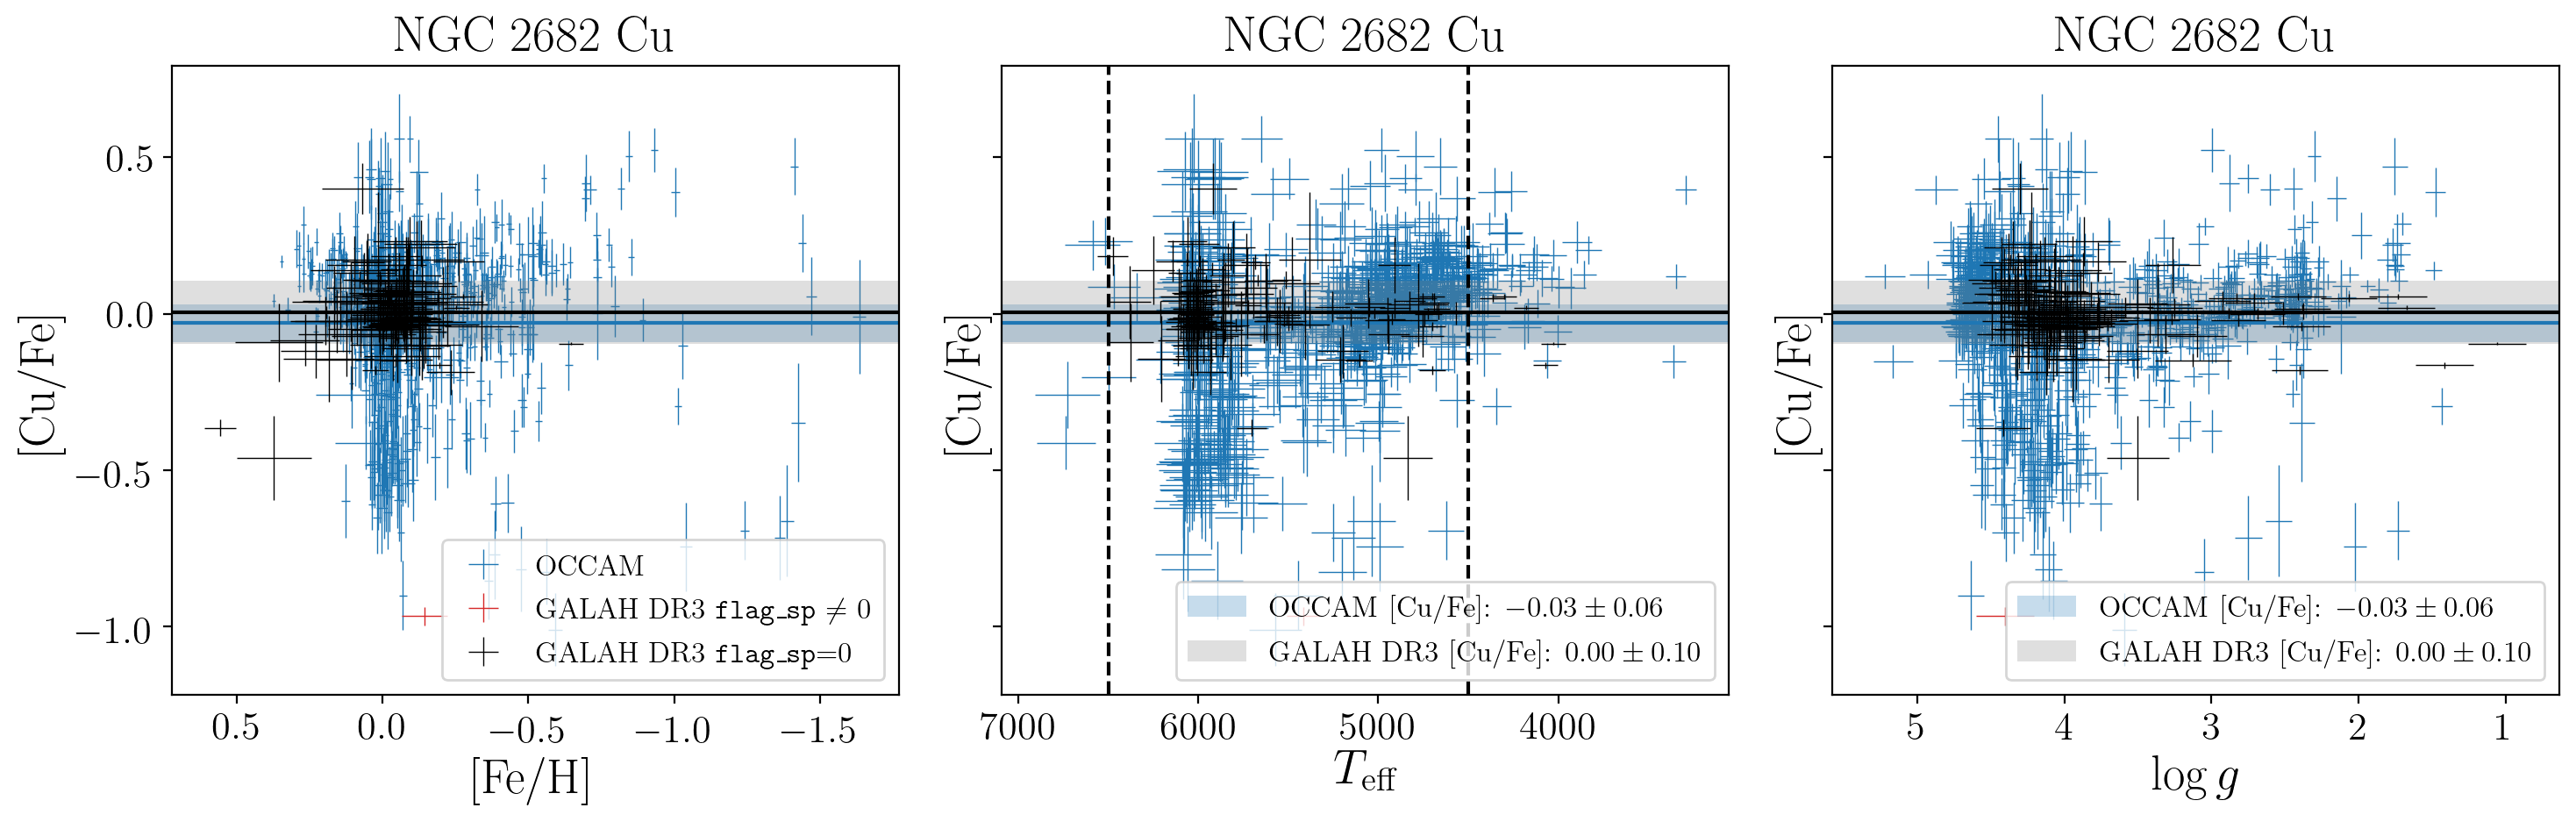
\includegraphics[width=0.49\textwidth]{figures/oc_Cu_NGC_2682.png}
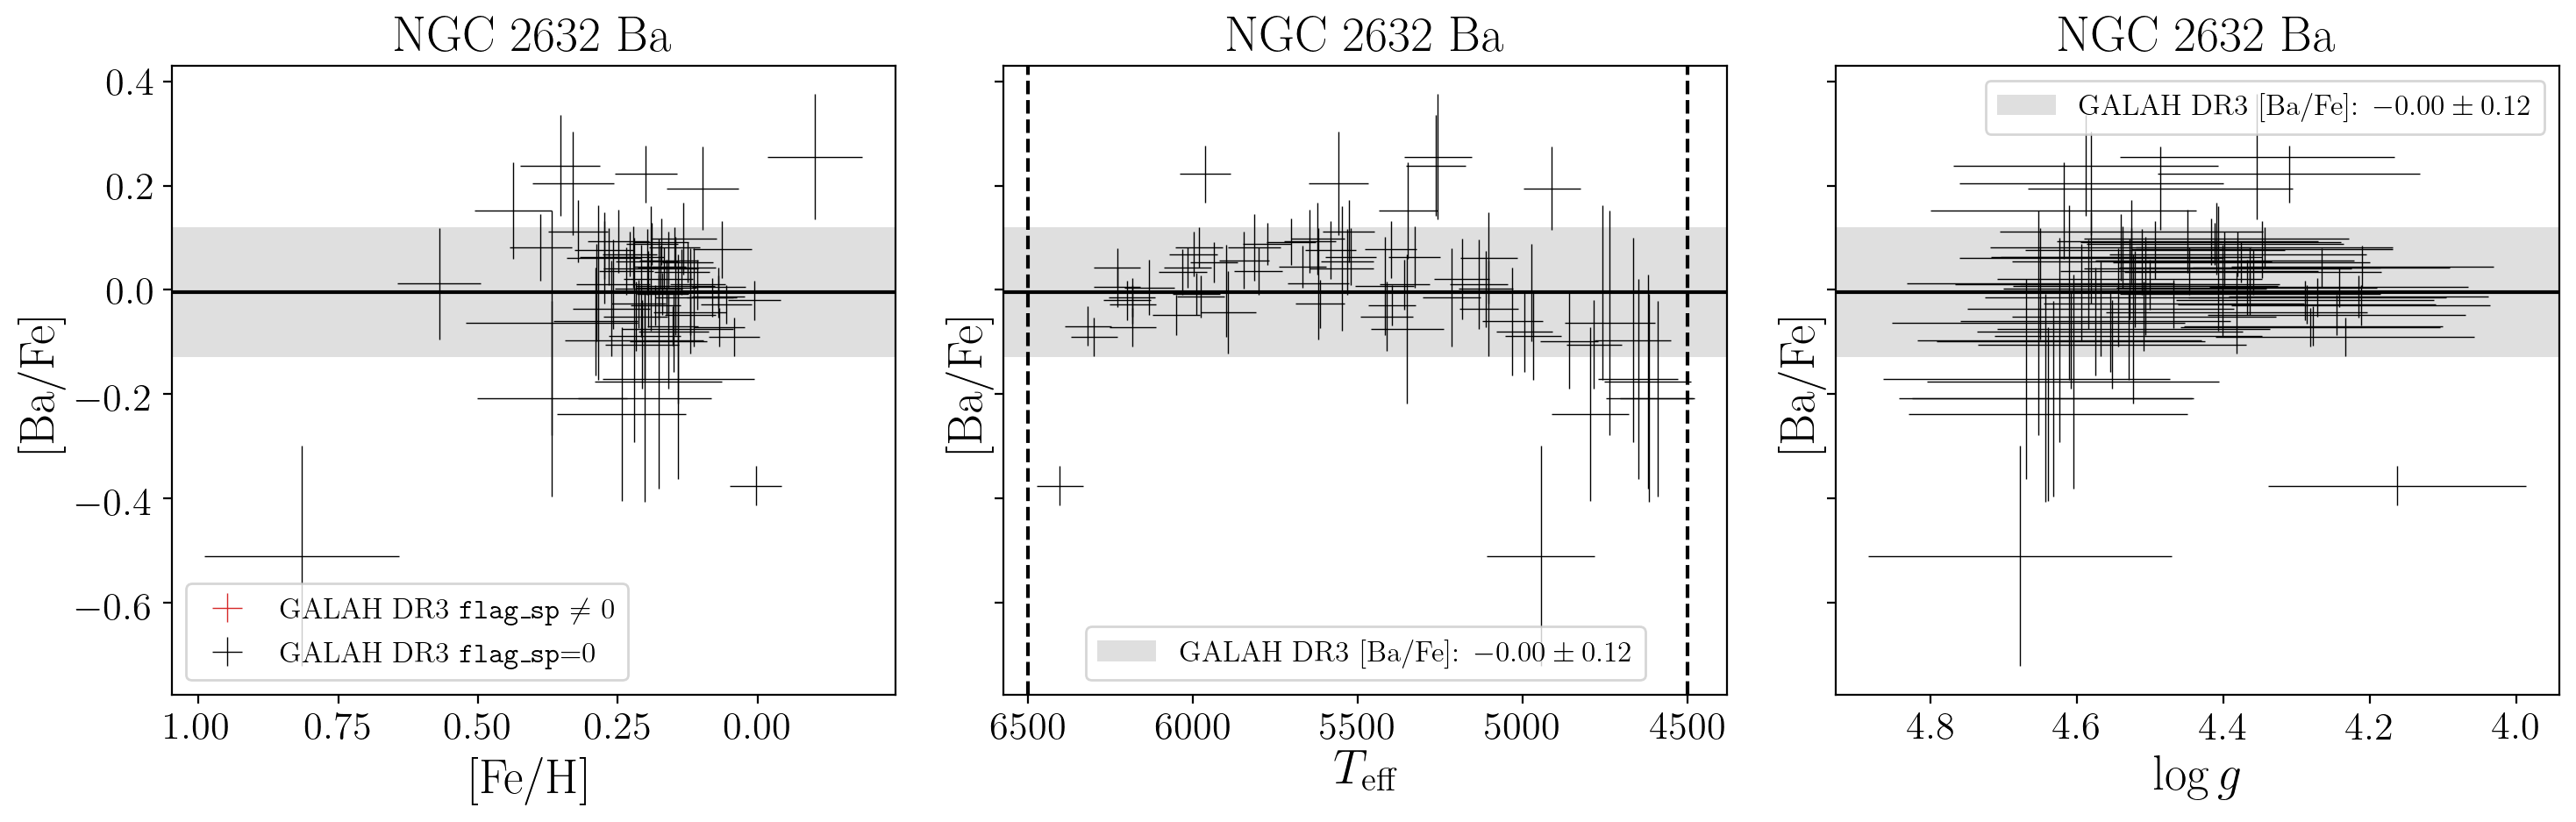
\includegraphics[width=0.49\textwidth]{figures/oc_Ba_NGC_2632.png}
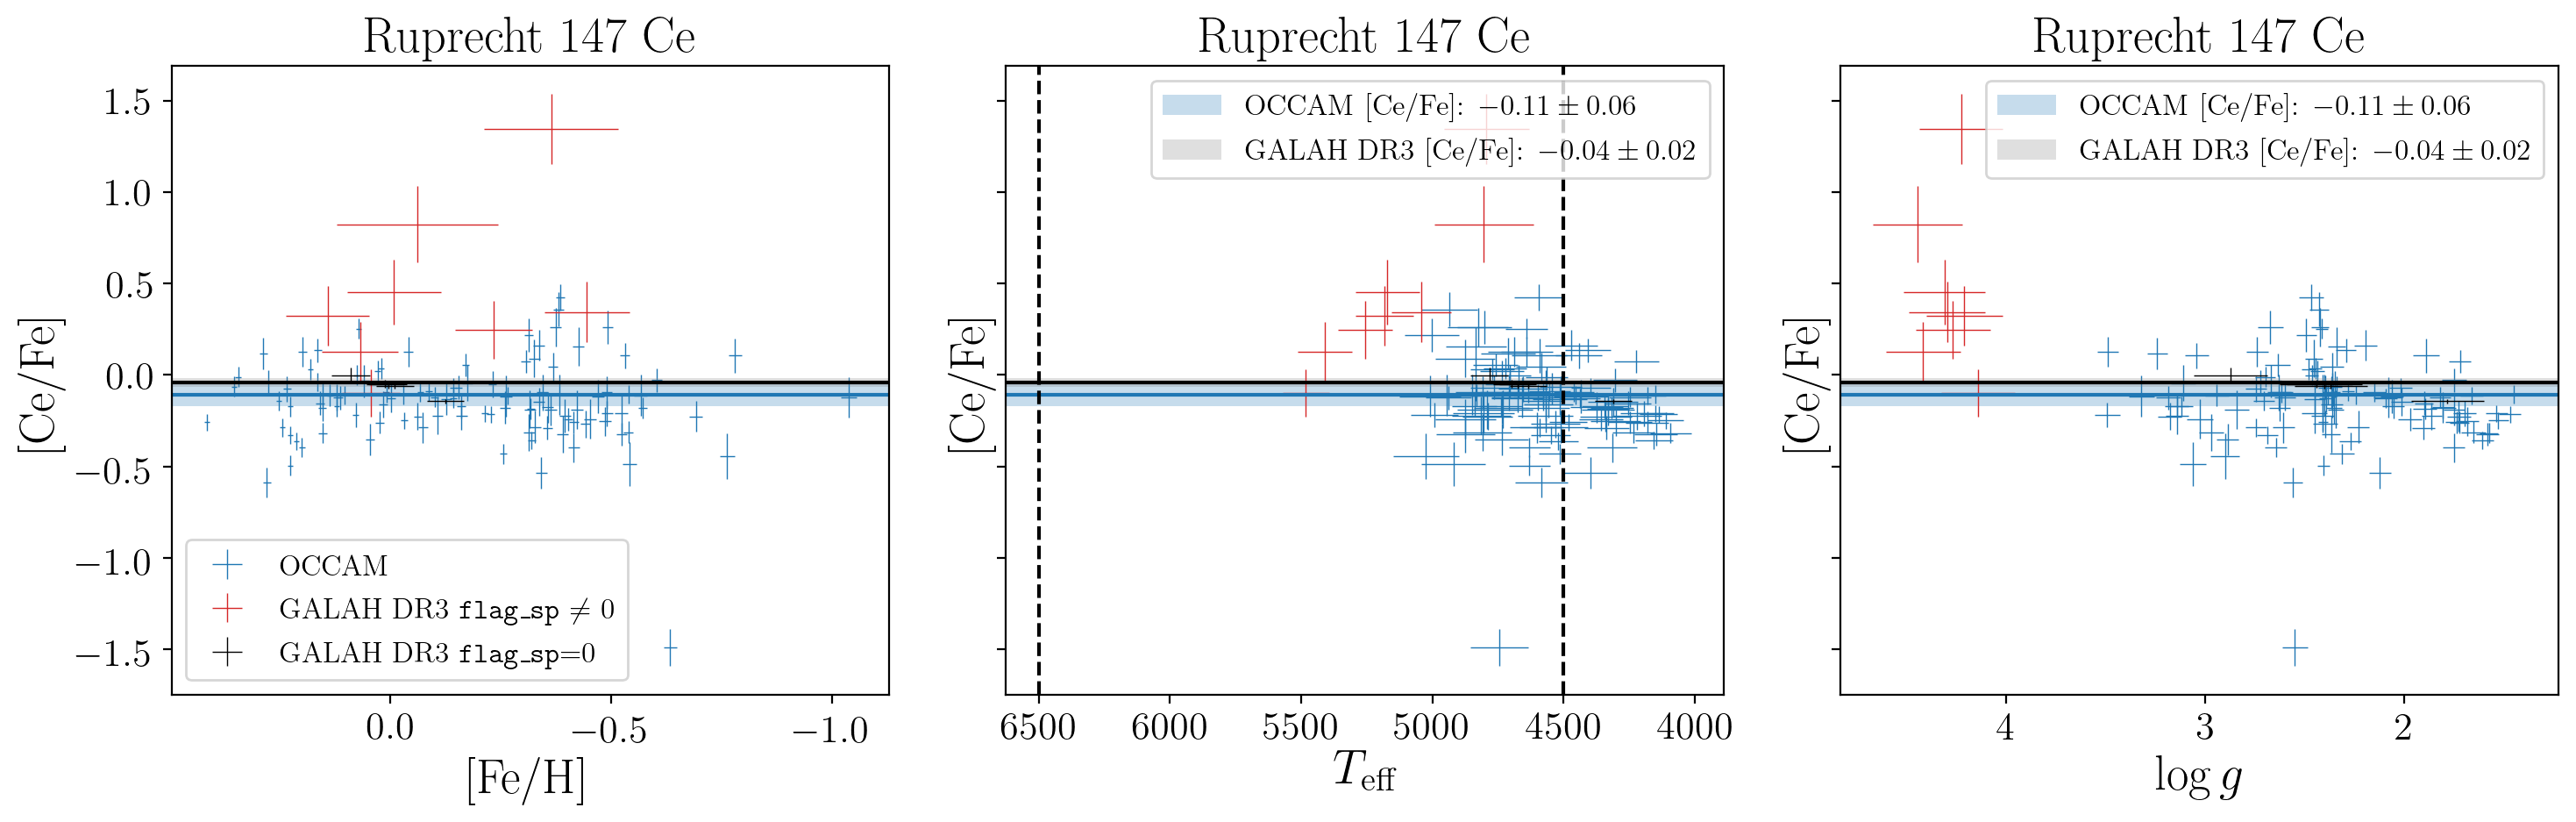
\includegraphics[width=0.49\textwidth]{figures/oc_Ce_Ruprecht_147.png}
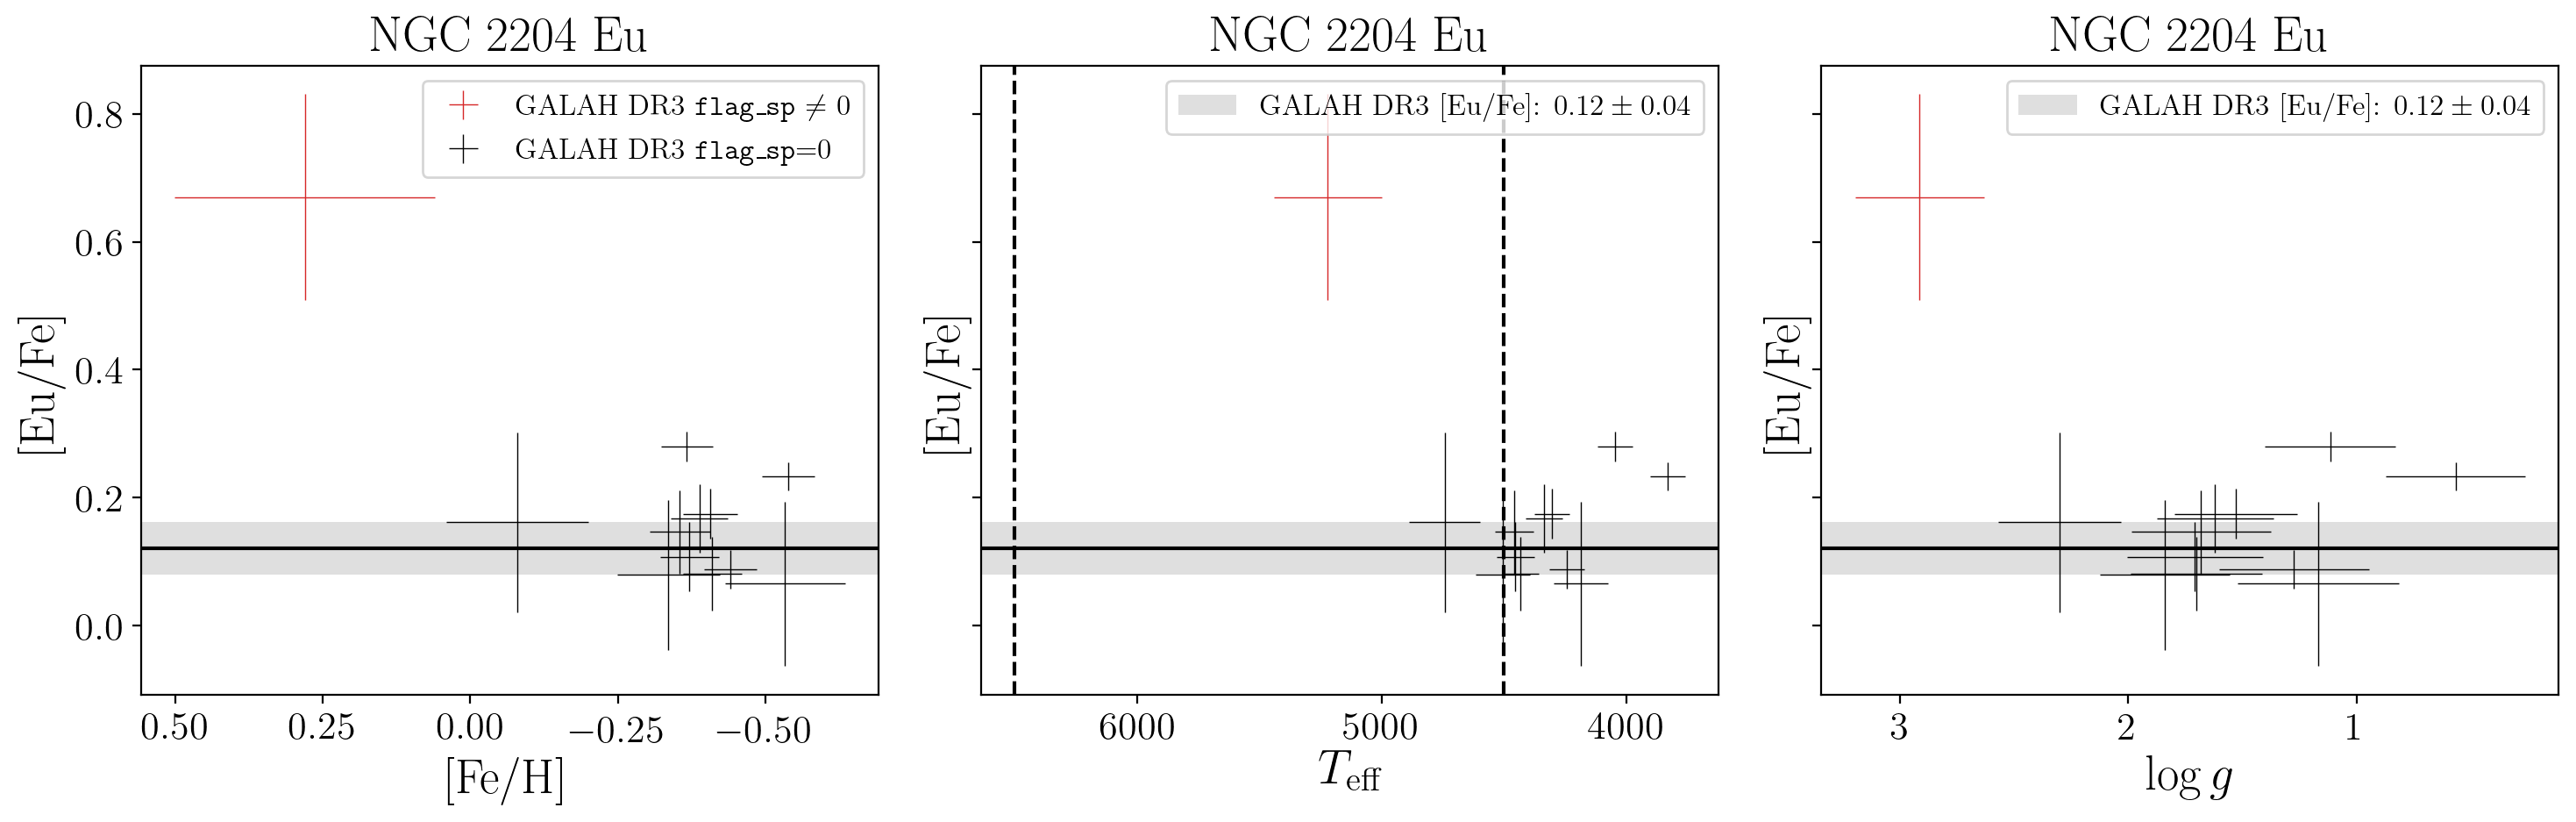
\includegraphics[width=0.49\textwidth]{figures/oc_Eu_NGC_2204.png}
\caption{Element abundances [X/Fe] as a function of stellar parameters \feh, \Teff, and \logg for a selection of elements X from the four clusters with information from both GALAH DR3 (unflagged in black, flagged in red) and the OCCAM survey \citep[unflagged data, blue][]{Donor2020} in Fig.~\ref{fig:oc_stellar_params}.  Horizontal bars indicate the mean abundances of the clusters from GALAH in grey (estimated from unflagged measurements of for stars with $4500 < T_\mathrm{eff} < 6500\,\mathrm{K}$) and the OCCAM survey (blue).}
\label{fig:oc_abundances}
\end{figure*}

\paragraph*{Element abundances of wide binaries}

Use \citet{ElBadry2018c} and select wide binaries from GALAH. We plot the difference in element abundances of the two components for different nucleosynthesis channels in Fig.~\ref{fig:wide_binary_ab}. For this comparison, we limit ourselves to those stars with similar [Fe/H] (within 0.25 dex) and similar \vrad (within 1 km/s). and no raised stellar parameter flags. We list their average differences in Tab.~\ref{tab:wide_binary_ab} together with their average quoted uncertainties.

\begin{figure*}
\centering
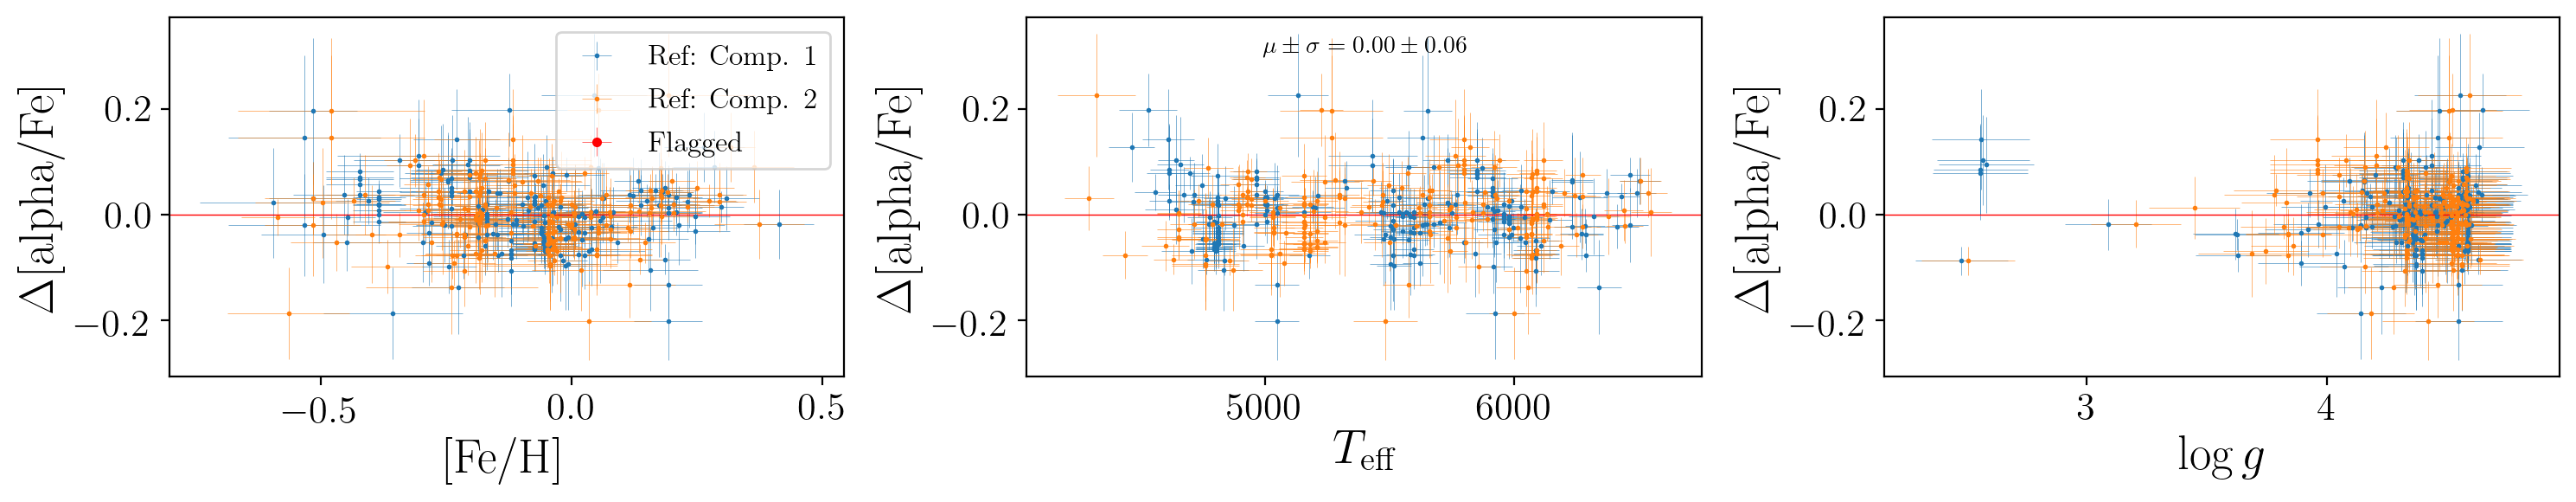
\includegraphics[width=\textwidth]{figures/wide_binaries_alpha.png}
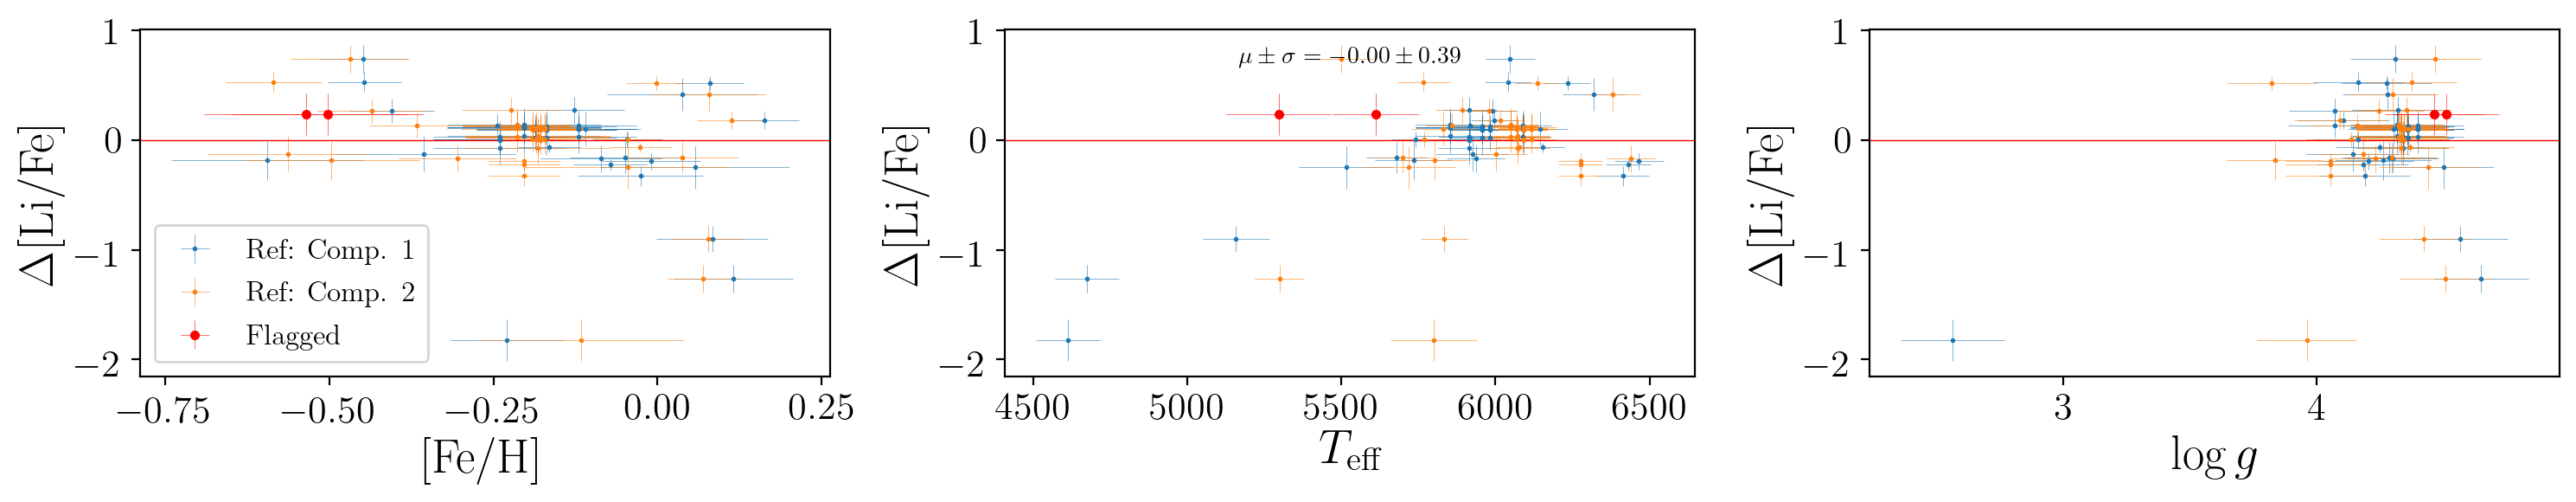
\includegraphics[width=\textwidth]{figures/wide_binaries_Li.png}
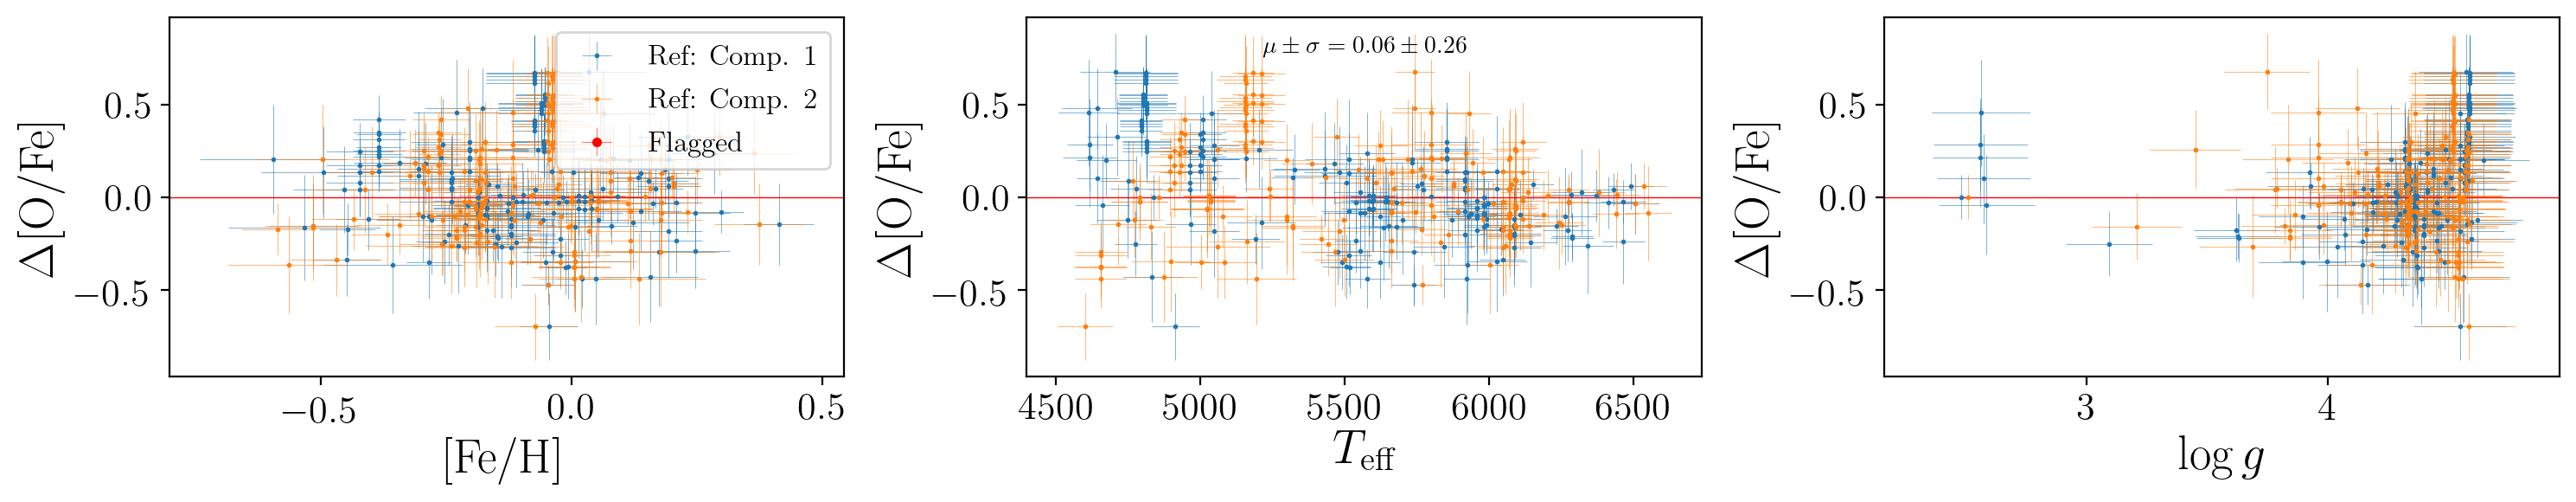
\includegraphics[width=\textwidth]{figures/wide_binaries_O.png}
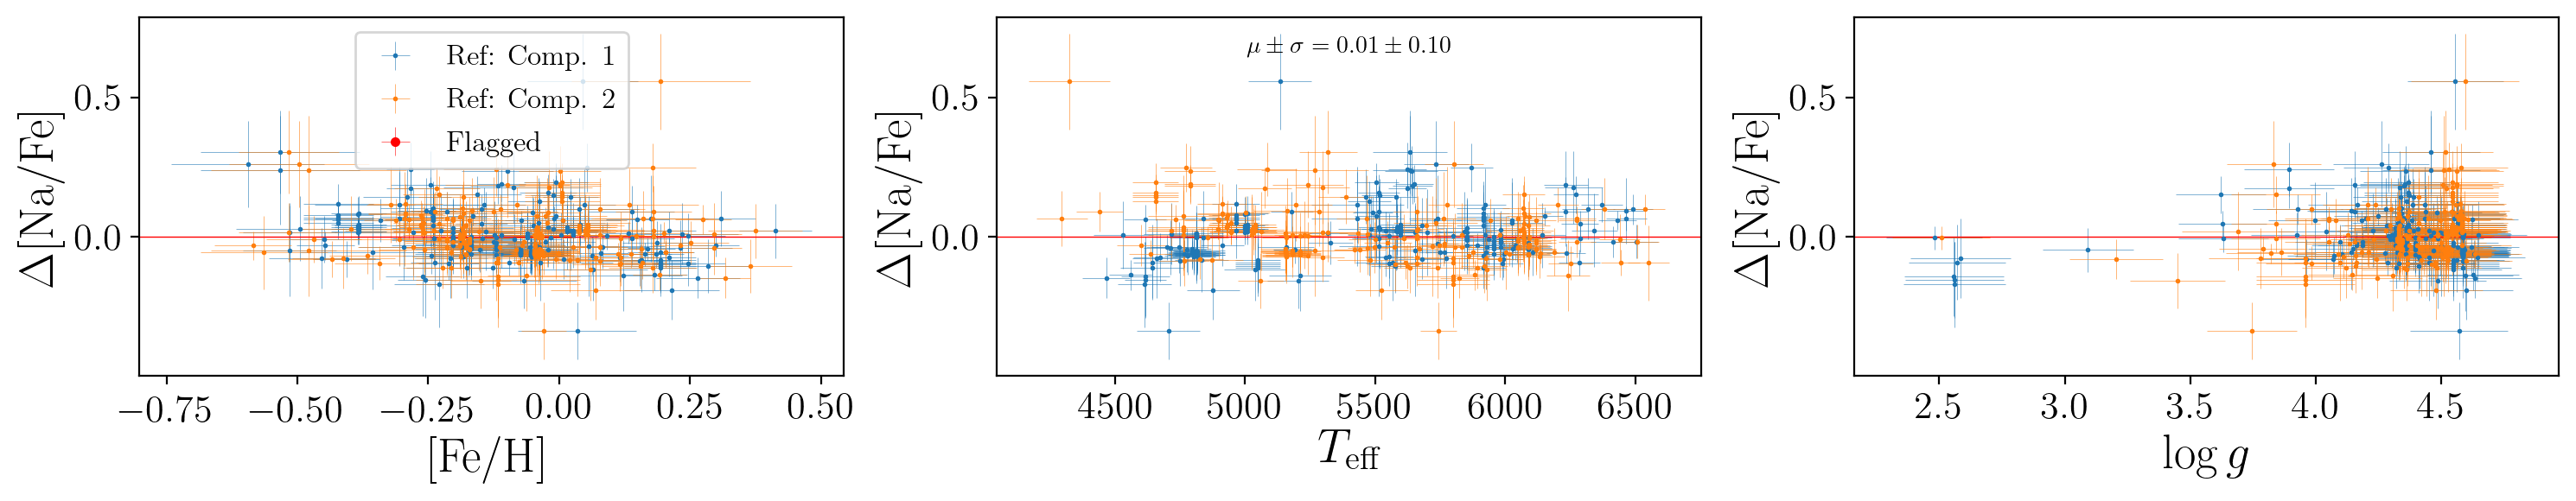
\includegraphics[width=\textwidth]{figures/wide_binaries_Na.png}
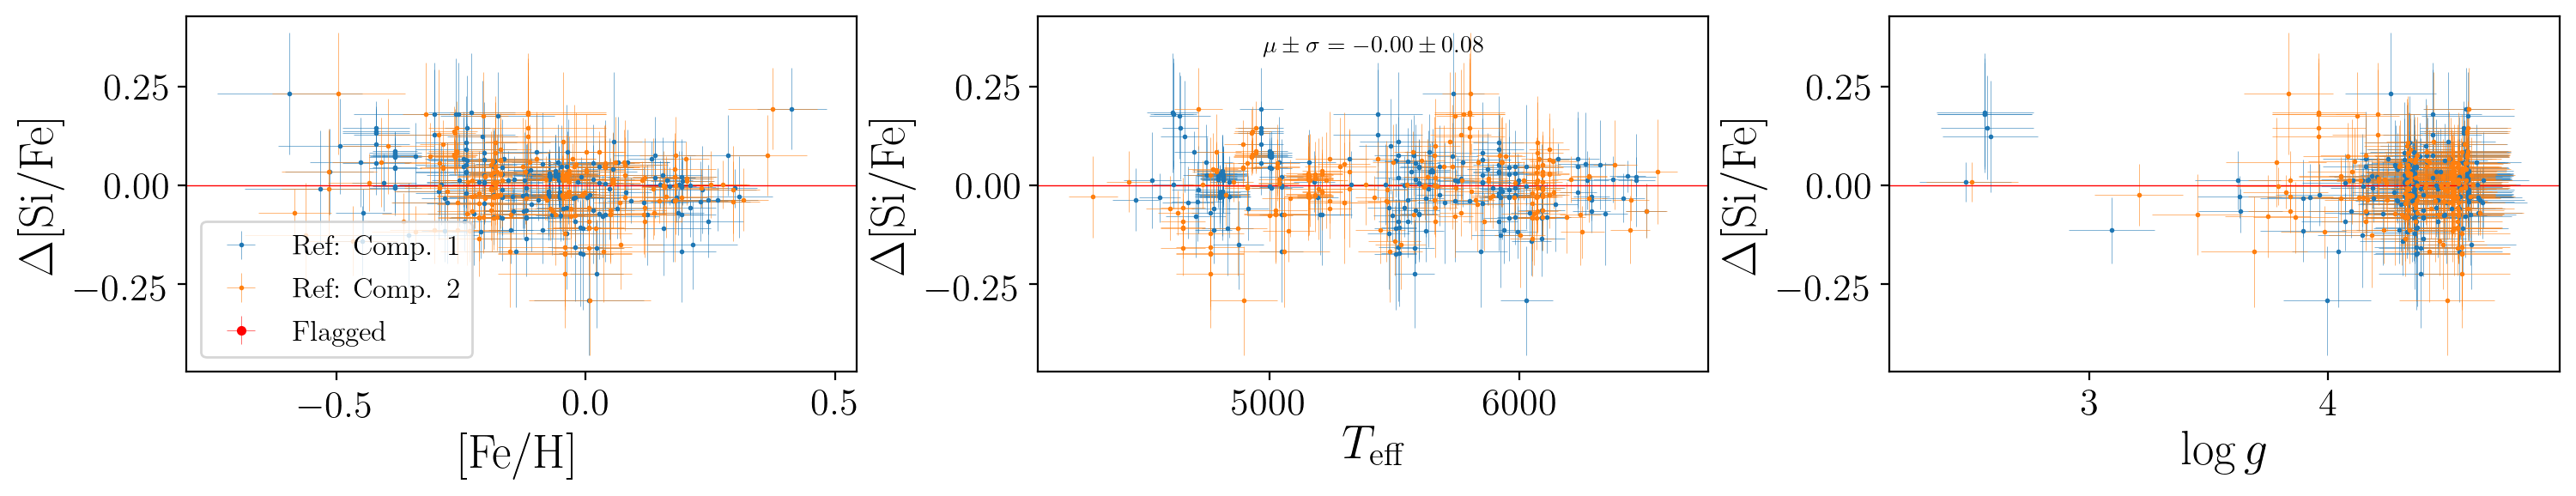
\includegraphics[width=\textwidth]{figures/wide_binaries_Si.png}
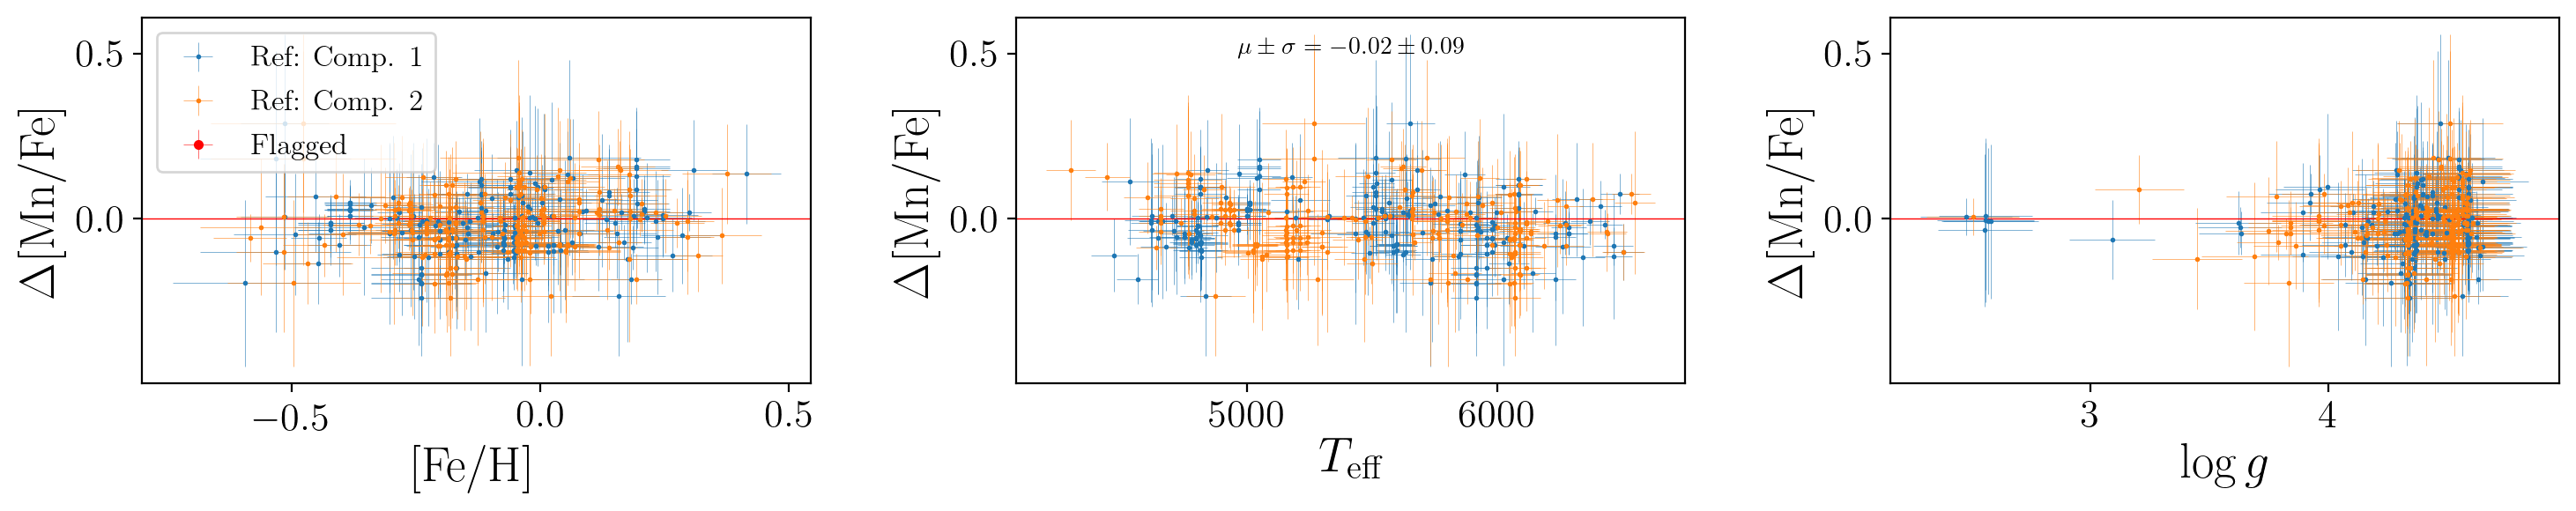
\includegraphics[width=\textwidth]{figures/wide_binaries_Mn.png}
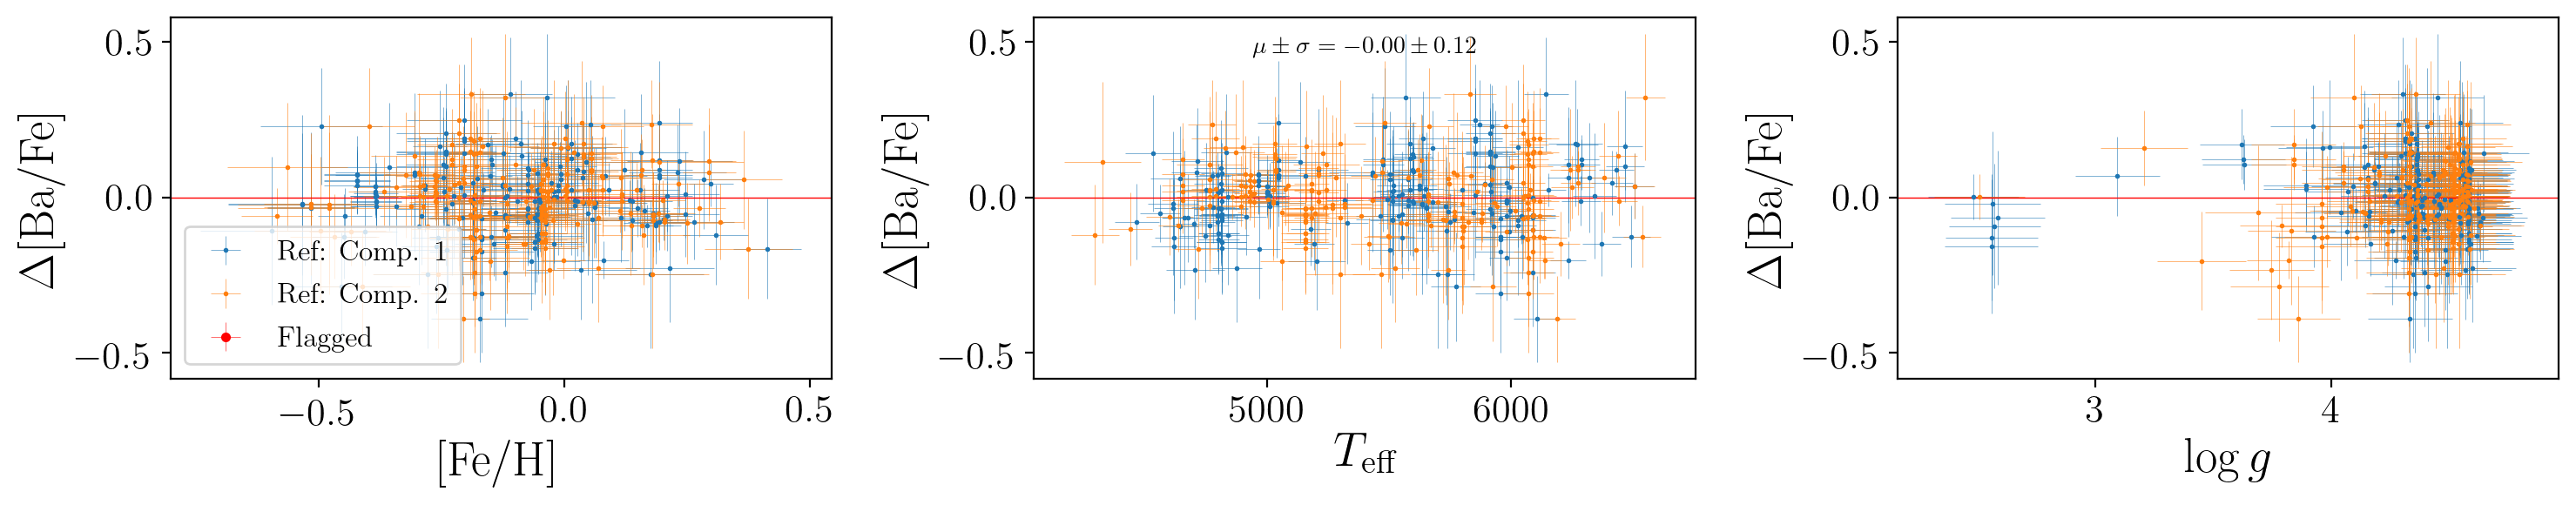
\includegraphics[width=\textwidth]{figures/wide_binaries_Ba.png}
\caption{Comparison of element abundances for wide binaries for the selected elements alpha, O, Na, Si, Mn, and Ba. Pairs were identified with the algorithm by \citet{ElBadry2018c}.}
\label{fig:wide_binary_ab}
\end{figure*}

\input{tables/wide_binary_ab.tex}

\subsection{Precision of element abundances}

We assess the precision by comparing the internal {\sc sme} covariance uncertainties with those from repeat observations of the same star in Fig.~\ref{fig:repeat_uncertainties_abundance_selection}. Contrary to the stellar parameter estimation, we see that the covariance errors from the individual line measurements are typically in good agreement for almost all lines. The standard deviations of the measurements are also consistent irrespective of the fibre combination. 

We note however that the finally estimated internal {\sc sme}-based errors are lower than the those from the repeat observations, when a large number of lines is fitted combined rather than line-by-line. This suggests that either the {\sc sme}-internal method has problems to estimate realistic errors when many pixels are involved or our spectrum quality indicator (\texttt{snr\_c2\_iraf}) is not representative in those cases. Contrary to the stellar parameter estimation, we only report the final abundance error from the raw internal covariance error, but provide the information for the repeat observations and covariance errors to allow a rescaling of the final uncertainties.

\begin{figure*}
\centering
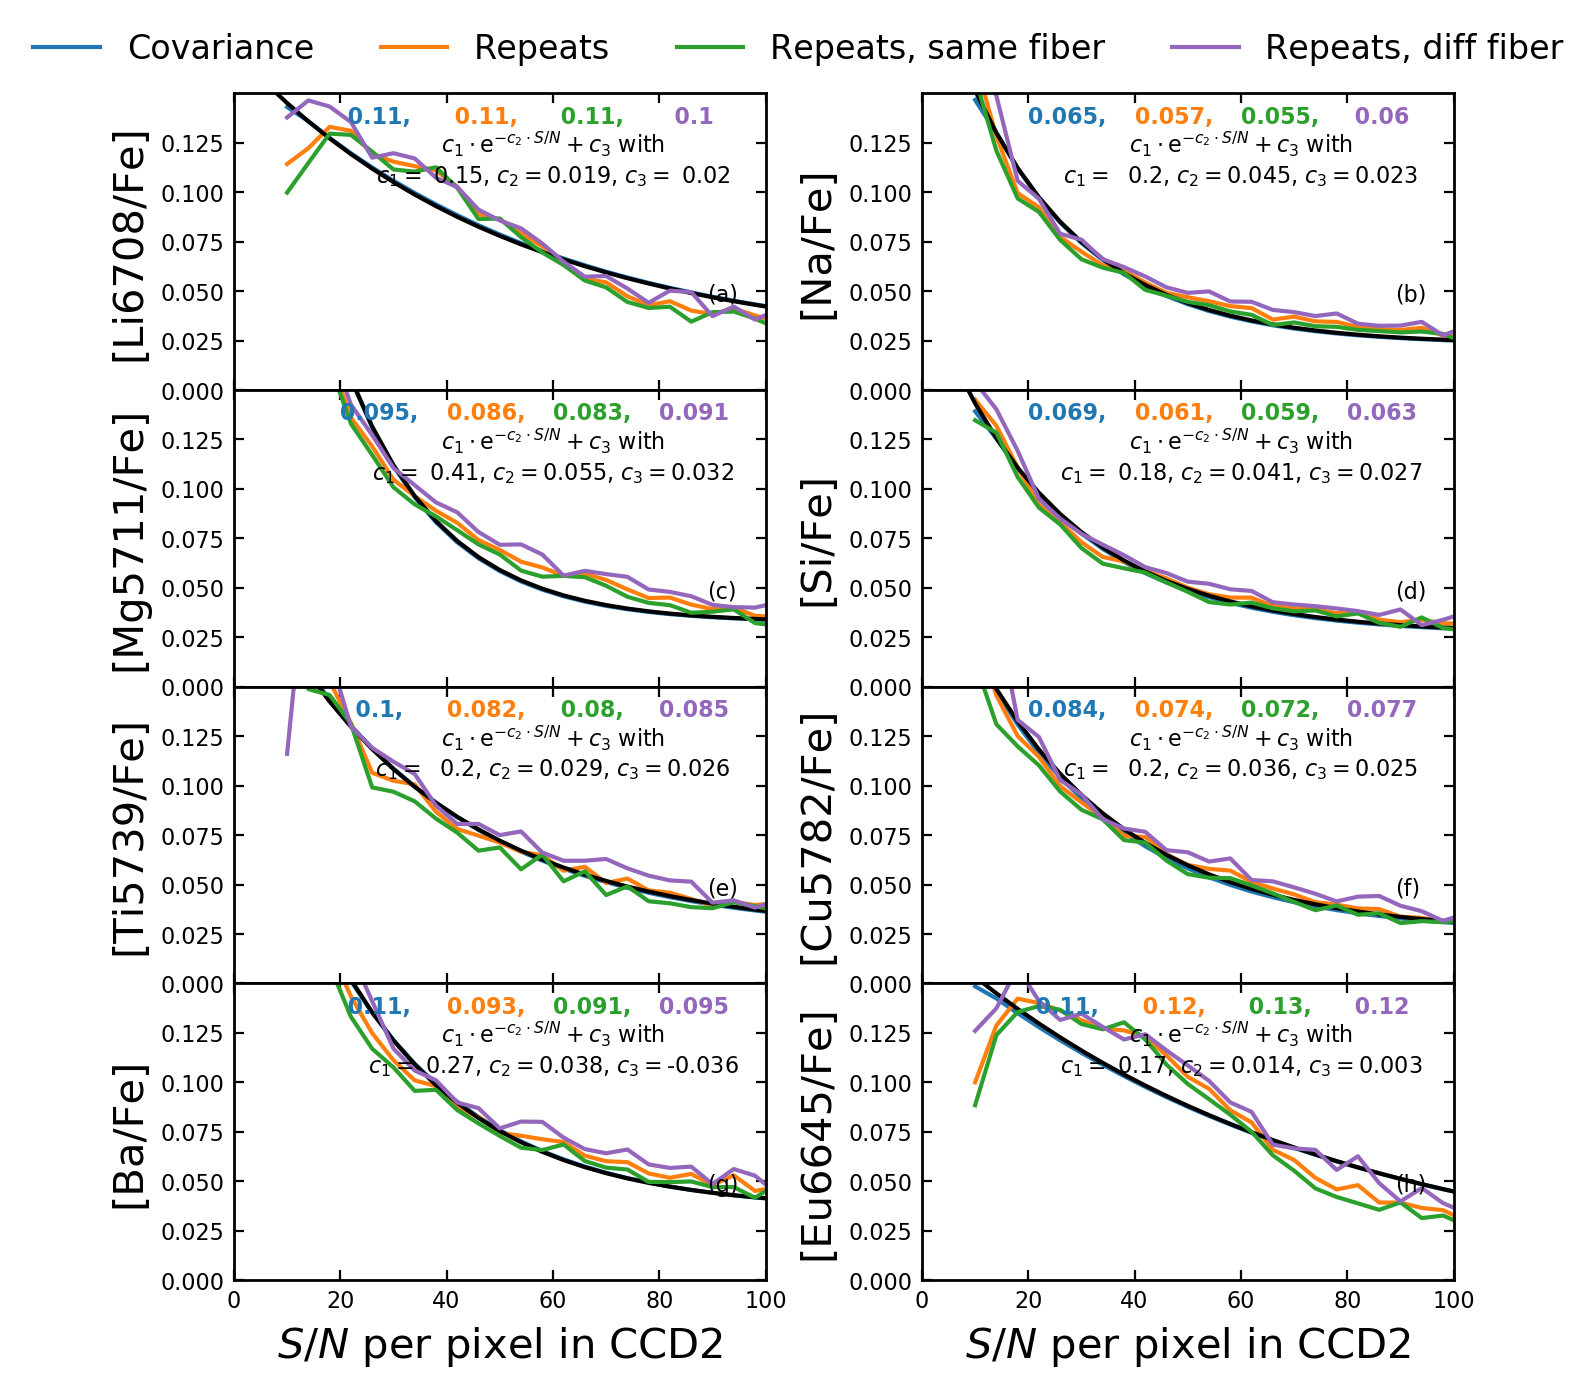
\includegraphics[width=\textwidth]{figures/repeat_uncertainties_abundance_selection.png}
\caption{Standard deviation of element abundances for eight different elements / lines in different bins of $S/N$ ($\texttt{snr\_c2\_iraf}$). Shown are the mean (internal) covariance fit uncertainties from {\sc sme} (blue), as well as the standard deviations for repeat observations of the same star for all fibre-combinations (orange), same fibre combination (green) and different fibre combinations (purple). An exponential function (black) was fitted to all (orange) repeats was performed. Number in the top state the expected or mean uncertainty at $\texttt{snr\_c2\_iraf} = 40$.}
\label{fig:repeat_uncertainties_abundance_selection}
\end{figure*}

Additionally, we assess the precision of element abundances for selected clusters with numerous observed members. These are however not useful in a straight forward manner to estimate the precision, due to internal processes like atomic diffusion and dredge-up changing the observed photospheric abundances for different the evolutionary stages and are not taken into account for the estimation of our precisions. Similar to GALAH DR2, we 

\SB{Estimate precision for several parameter ranges for NGC~2682 (M~67), and maybe also Ruprecht~147 which cover both dwarfs and giants. List those in a table. Mention that difference in [X/Fe] between the evolutionary stages is a physical difference of surface abundances with reference to \citet{Gao2018, BertelliMotta2018, Souto2018, Souto2019}.}

\subsection{Flagging of element abundances}

As for all data release, we want to stress that we discourage the use of flagged element abundances without consideration of the possible systematics, that these flagged measurements can introduce. We expect less trends without the influence of the training set selection or data-model flexibilities, but we still expect trends for several reasons.

Given the model- and setup-imperfections, excluding \logg as a free fitting parameter might lead to systematic trends. This can be the case for those stars where the true \logg of the star and our estimated \logg differ significantly (e.g. binaries where the (unidentified) second component is contributing to the flux of the system) or the synthetic spectrum with the true \logg does not match the observation (e.g. due to shortcomings of the 1D model atmospheres and synthesis).

For stars with more lines, our pipeline will perform worse several ways. Firstly, estimating the continuum will be less reliable. Secondly, we will run into issues of strong blending, where our estimate is limited to how close the synthesis of the blending lines is to the true observation. If for example a star has scaled solar abundances, our estimates of the element abundances will still be good even for blended cases. If the compositions differs, and the line that we want to measure is blended by a line of a significantly over- or under-abundant element (relative to scaled-solar), our measurement might be corrupted. We try to limit this by performing a blending test, but setting the limit on how much blending is still acceptable is both non-trivial but also hard to flag during post-processing.

Due to time/computation restrictions, we were running several elements in a combined rather than line-by-line basis, which can decrease the precision as outlined in Sec.~\ref{sec:analysis_flow}, although we have tried to ensure that the abundance zeropoints of the individual lines were similar for those elements that were run with the combined setup.

\section{Possible caveats: analysis shortcoming or physical correlation?} \label{sec:caveats}

In the previous sections we have laid out our approaches to flag unphysical results and spectra with peculiarities for which our pipeline is likely to underperform. However, these approaches are all of a rather automated routine, because we can not inspect all of the more two million measurements that have been performed for this data release. Furthermore can not dig into all the details of possibly unexpected correlations as many of these are posing problems to understand the possible astrophysical nature of these trends (as previously shown for atomic diffusion causing systematic differences of surface abundances in open cluster stars).

In this section, we are thus addressing several possible caveats, for which we are not convinced, that these are analysis shortcomings or true physical correlations. We give examples for peculiar abundance patterns and show an example, where the pattern (of Am/Fm stars) is truly representing the observed surface abundances when assuming ionisation equilibrium. In other cases, especially for the most metal-rich as well as coolest giant stars, we are aware that our pipeline is likely introducing systematic trends, because our synthetic spectra do not include all molecular line information, the line data of these lines is partially uncertain, and we are facing the problem that we do not have true continuum points to use for the spectrum normalisation in these stars. In the latter case, the pseudo-continuum placement can correlate strongly with the stellar parameters (especially [Fe/H]) and lead to systematic trends in the reported measurements. We address possible influences on the reliability of surface gravities and finally also lay out considerations of the uncertainties and how these will be improved in future data releases.

\subsection{Systematic and peculiar abundance patterns}

\SB{Michael will contribute some description for the most metal-rich giants}

\paragraph*{Influence of astrometry/photometry on abundances}

\SB{This is what YST mentioned in his email from 200402: When the star is not a single star (and the second component is contributing significantly to the flux or when the parallax is uncertain and the Bailer-Jones prior puts the star at a smaller distance than in reality, this introduces systematic trends in the surface gravity, but thus also in the abundances.}

\paragraph*{Atmosphere composition for spectrum synthesis}

Follow up with comment from YST, that we assume the abundance pattern of all stars to be scaled-solar during the stellar parameter phase and the abundance fit (only adjusting one abundance).

This is dangerous, if the true abundance pattern deviates significantly from the solar pattern, because it not only influences individual lines, but also molecular equilibrium and thus can have drastic consequences for the continuum and molecular line strengths. I guess a reference to YSTs Payne paper and the O from atomic and molecular features would be good here to remind the reader of that issue.

\paragraph*{Chemical composition of Red Clump stars}

Fig.~\ref{fig:Ba_RC_RGB} shows that the RC stars have systematically higher [Ba/Fe] than the RGB stars. In previous emails, Thomas Nordlander suggested that this might be a sign of non-scaled-solar abundance patterns for C and N, which are expected to be different. If these are very different, our scaled-solar atmosphere composition is not accurate. Interestingly, Ba is more affected by this than e.g. Y. We see Na, Al, Sc, Ti2, Ni, and Ba more enhanced at metal-rich end.

\TN{There are of course MARCS models available that take into account CN mixing. Some time before DR4, it might be worth doing a synthetic test with these to see what kind of biases we'd expect introduced from the mixing. I don't know what would be the best reference for CN mixing, but e.g. Fig 7 of \citet{Tautvaisiene2013} shows that already ~solar mass red clump giants have significantly lowered C/N ratios, so probably all of them are affected by this! If it turns out [Ba/Fe] is a good tracer of CN mixing, then that in itself would be valuable.}

\AMA{Thanks for the plots.  I checked our smaller 50k sample, and the line-by-line dispersion for [Ba/H] does not stick out for the RC compared to the RGB, compared to how [Ba/H] itself sticks out.  This might suggest it is a real result; however Sven's plot earlier suggests both are strongly saturated, so maybe we cannot draw conclusions from it. As I think Thomas said, it would be good to eventually check the impact of CN mixing using one of the CN-cycled MARCS models -- the synthetic line strengths just need to be compared in one or two test cases.  The dip in [Al/Fe] is also curious (at least to me)... but maybe it is nothing. Regardless of whether or not a Ba enhancement actually exists in these RC stars, the measured Ba enhancement seems quite real in the realm of standard marcs models; it is an interesting result, I think, that hasn't been discussed in the literature before (as far as I can tell...?).  If it is to be measured in the caveats, perhaps this paper discussing formation depths would be helpful: \citet{Gurtovenko2015}.  In the Sun, the 585.4nm and 649.7nm lines have the same excitation potentials (0.604 eV) but the former is somewhat weaker (log gf=-0.907 compared to -0.407), so it forms slightly deeper in the atmosphere.  However, both form extremely high: $\log \tau$ of around -3 and -5 (according to the table at the end of the paper; $D_{l}$); hence why these lines may be sensitive to the effects Thomas mentioned, whereas the other lines in GALAH may not be so sensitive.}

\begin{figure*}
\centering
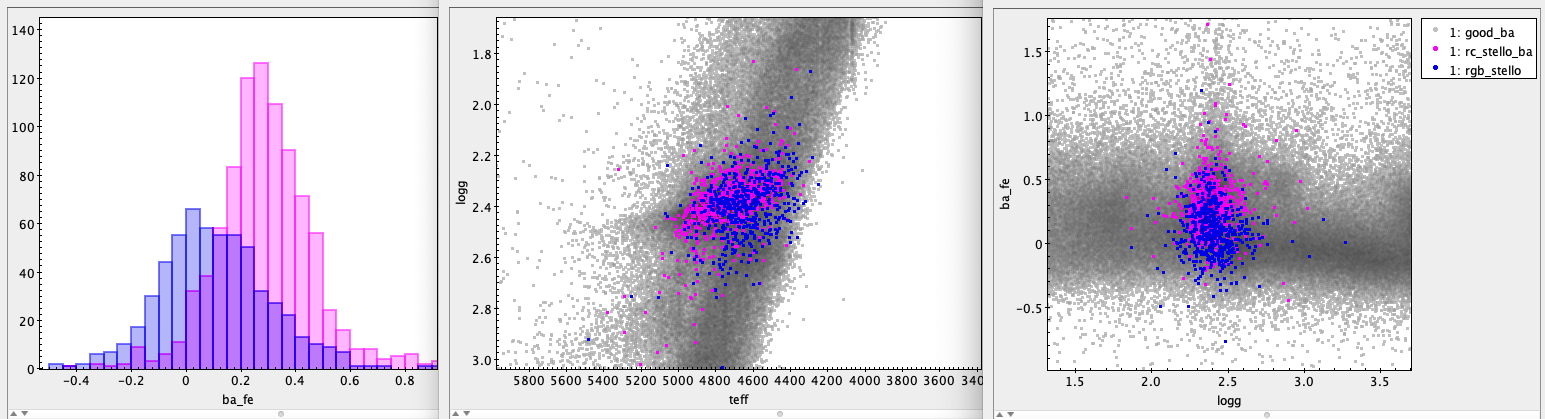
\includegraphics[width=\textwidth]{figures/Ba_RC_RGB.png}
\caption{Figure from Email from Jeffrey Simpson on 200428, showing that the RC (identified via K2 asteroseismic classification by Dennis Stello) has significantly higher [Ba/Fe] than the RGB (again identified via K2 asteroseismic classification).}
\label{fig:Ba_RC_RGB}
\end{figure*}

\paragraph*{Abundance patterns of Am/Fm stars}

We and others (e.g. \citet{Xiang2020}) have found them and our pipeline estimates abundance patterns of  \citet{Fossati2007,Fossati2008}, see their Figs. 11 and 12. 

However, we want to stress that our pipeline is not adjusted for the analysis of such stars, and our approach of assuming ionisation equilibrium might fail in these stars and their abundances might thus be wrongly measured. 

Fig.~\ref{fig:GALAH_DR3_AmFmStars}

\begin{figure*}
\centering
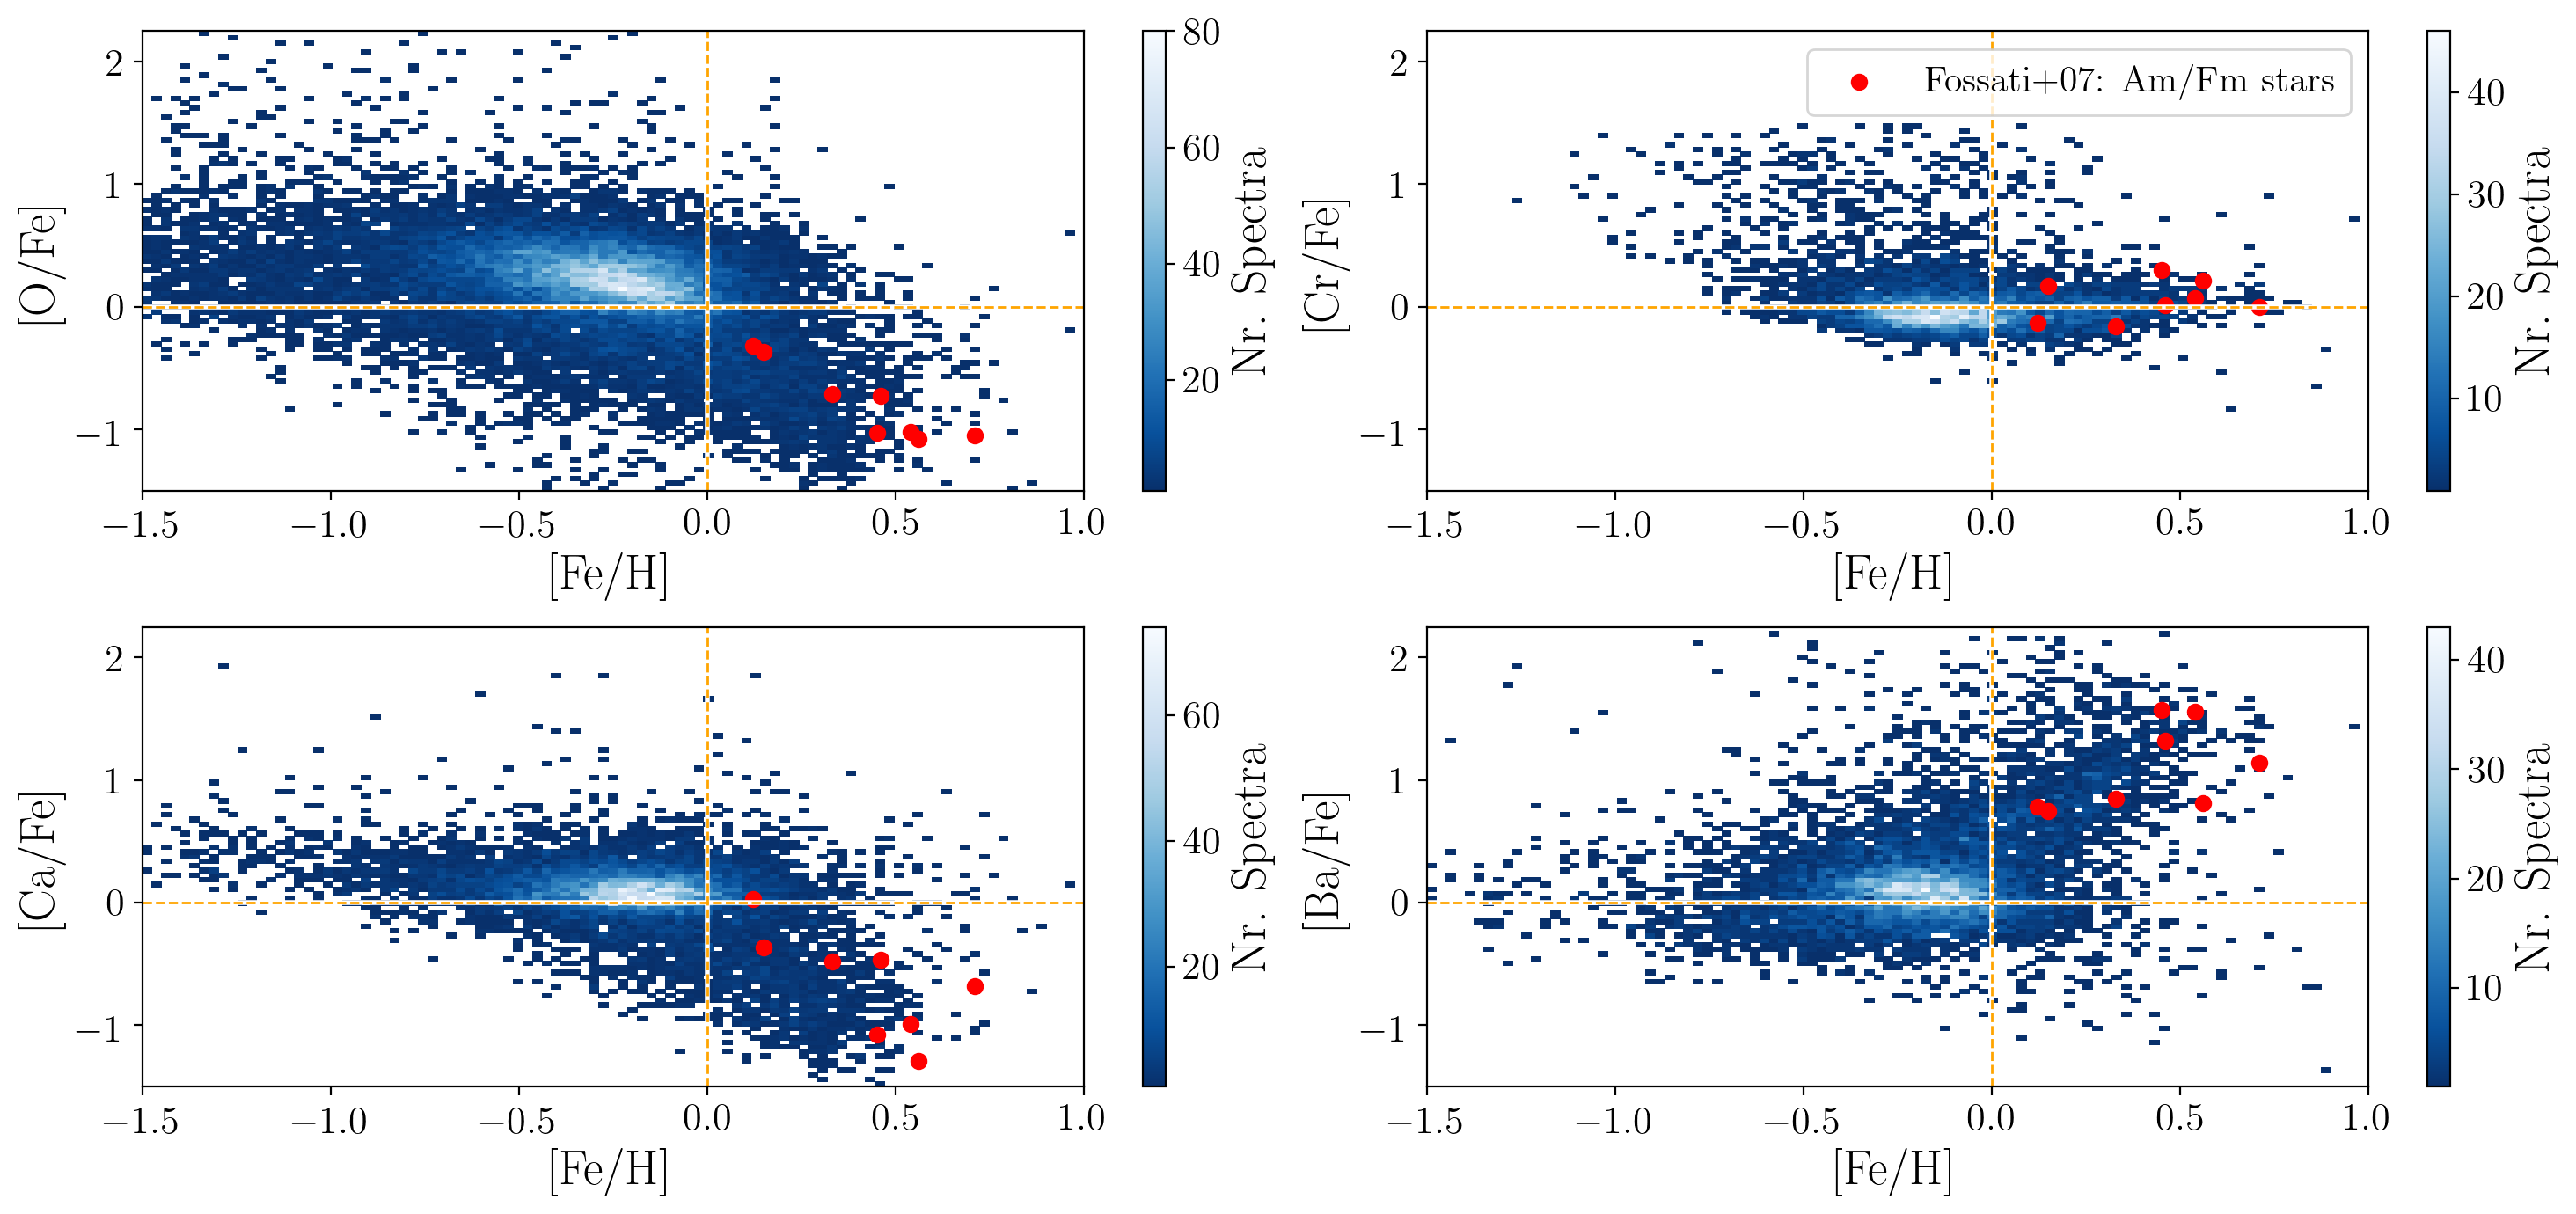
\includegraphics[width=\textwidth]{figures/GALAH_DR3_AmFmStars.png}
\caption{Element abundances [O/Fe], [Ca/Fe], [Cr/Fe], and [Ba/Fe] for GALAH stars with $T_\text{eff} > 6500\,\mathrm{K}$. Overplotted are studies of Am/Fm stars by \citet{Fossati2007} in red.}
\label{fig:GALAH_DR3_AmFmStars}
\end{figure*}

\paragraph*{Metallicity trends in clusters}

In clusters, we see a strong trend of temperature with metallicity. Could this be caused by our prescription of vmic? See paper by \citet{Baratella2020} who find that vmic is overestimated and thus [Fe/H] is underestimated when using Fe lines in clusters.

\paragraph*{Over-/under-densities around atmosphere grid points} Overdensities at 3500 and 4750..(250)..8000K. Underdensities below 4750

\paragraph*{Metal-rich giants} True issue of stellar models? We have seen issus with metal-rich giants in DR2 already (unphysical location of RC). Models are incorrect for metal-rich giants due to missing/unreliable molecular lines? Blending criteria not conservative enough? Continuum estimation very hard due to missing continuum points and being left with metallicity-sensitive pseudo-continuum.

\paragraph*{Cool RC end} This issue was identified via clumps in element abundances (e.g. two low [O/Fe] clumps) at the cool end of the RC. In this area, we might mis-identify RC stars as RGB stars due to a lack of appropriate RC clump isochrone entries. The underestimated mass might thus lead to an underestimated $\log g$.

\subsection{Reliability of surface gravities}

\paragraph*{Binarity}

\citet{PriceWhelan2020} We expect way more binaries for the hot stars (see their Fig. 5).

\paragraph*{Isochrone choice for mass estimation} We could select better isochrone sets in terms of 1) finer sampling (especially for younger stars), 2) treatment of alpha-enhancement (expanding the isochrones by those which have been calculated with alpha-enhancement) 3) stellar physics treatment like atomic diffusion 4) age choices beyond the age of the universe (for more reliable age uncertainty estimates)

\paragraph*{Cool stars}
Mass uncertainty due to isochrone choice \citep[see discussion e.g. in ][]{Heiter2015}. Also: Isochrones end at a certain luminosity?

\paragraph*{Scattering in Potassium} Due to interstellar Potassium? include flagging (if not done for DR3) by checking expected equivalent width via $W = f(E(B-V))$ relation from \citet{Munari1997} High [K/Fe] especially for RC stars. Systematics or physical effect (does not seem to be correlated with high A(Li)?

\paragraph*{Stars with high extinction} Stars with high extinction will have uncertain logg. Flag them?

\paragraph*{Overdensity around 4650K, 4.7dex} Isochrone issue

\paragraph*{Noding in ages and masses} in ages due to chosen linear age grid 0.5..(0.5)..13.5 Gyr. This effects the hot stars and secondary RC. But why nodes in masses (for cool main sequence)

\paragraph*{Young star parameters} mass estimates possibly poor due to isochrone grid selection? vmic is not free, but tied to a relation. rotational broadening. Deviates strongly from true vmic? Line shape strongly influenced by activity?

\subsection{Assessment of uncertainties}

\SB{Elaborate here what this could and should be done better, i.e. by assessing the accuracy as a function of different stellar parameters. Stress also that these are however hard to get, because the external informations (e.g. angular diameter measurements) are typically limited to very nearby stars. Need a bridge for the typical magnitude ranges of GALAH (and other ongoing surveys). We would welcome more work in this direction (write down to give Gregor and Diane more evidence that the community needs this)! Also caution, that using other surveys as validation is not ideal, because they also are effected by systematic trends. Bottom line: we do the best we can to use external information from angular diameters, bolometric flux, IRFM, and other sources to validate. Use other surveys or studies (e.g. solar twins and clusters) to allow the user to assess possible systematic trends.}
\SB{Note that in the future (DR4?), we will also work on using the $S/N$ within the line mask rather than the average CCD2 $S/N$!}

\paragraph*{Microturbulence} In the future it is worth to test implementing $v_\text{mic}$ as a free parameter or use the relations estimated by \citet{DutraFerreira2016} based on 3D atmosphere calculations. Whereas these agree with the empirical GALAH iDR3 relations for the majority of the stars within $20\%$, they differ significantly for the hottest and most luminous stars, for which GALAH iDR3 is currently not estimating the most reliable stellar parameters anyway.

Using $v_\text{mic}$ as a free parameter showed significant improvements of trends with $T_\text{eff}$ for the APOGEE survey \citep{Holtzman2018} and will be tested for the next data releases

\begin{figure*}
\centering
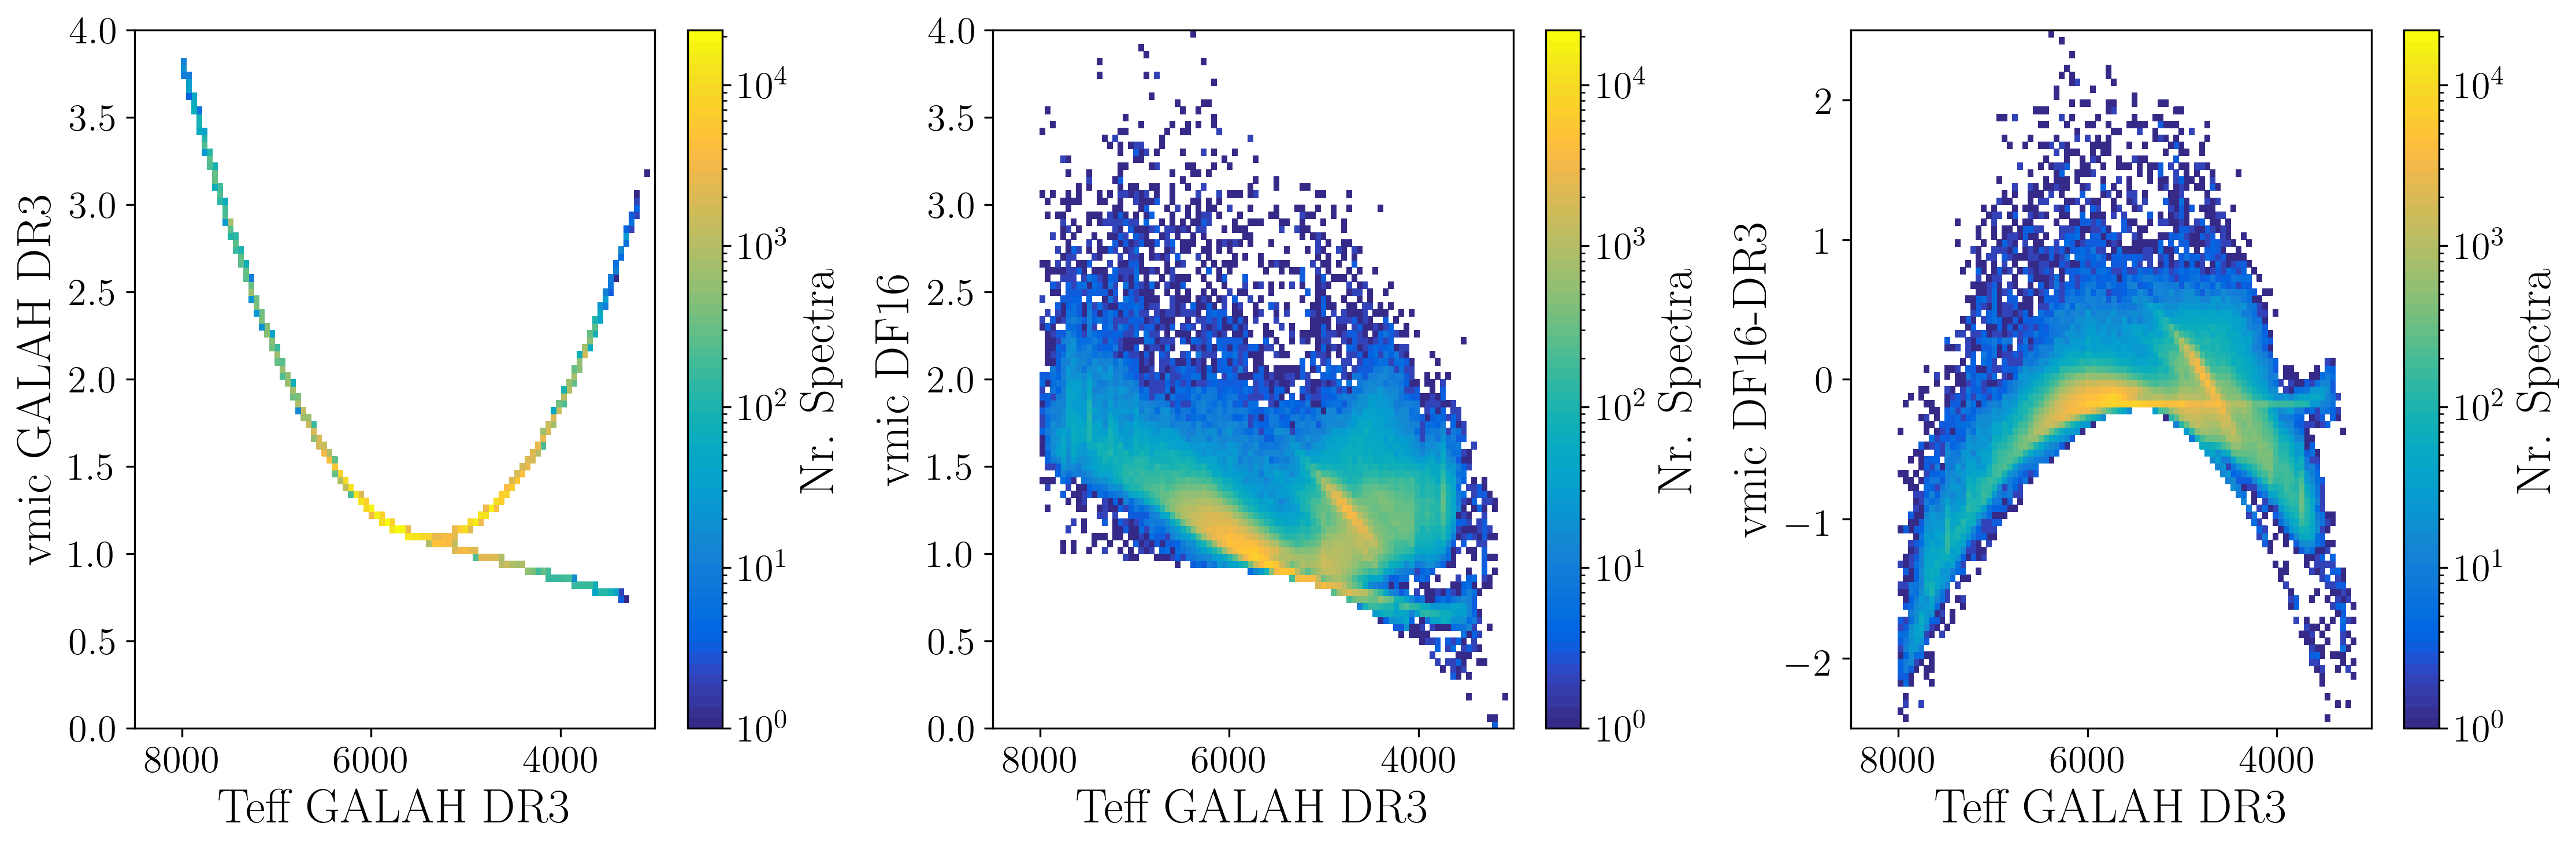
\includegraphics[width=\textwidth]{figures/Vmic_comparisons.png}
\caption[{Comparison of $v_\text{mic}$ calculated via relations used for GALAH iDR3 and \citet{DutraFerreira2016}}]{Relations of $v_\text{mic}$ as a function of $T_\text{eff}$ calculated via relations used for GALAH iDR3 and \citet{DutraFerreira2016} in the left and middle panels, respectively. A comparison of the two $v_\text{mic}$ values as a function of temperature is plotted in the right panel and shows good agreement for the majority of stars, i.e. cool and warm dwarfs and stars around the RC. However, the two relations disagree strongly for the most luminous and hottest stars. For the latter, GALAH iDR3 $v_\text{mic}$ values are up to two times higher.}
\label{fig:vmic_comparison}
\end{figure*}

\paragraph*{Extinction} we could estimate $A_X$ via SED fitting rather than just relying on the RJCE method or $R_{K_s}$*E(B-V)

\section{Catalogs included in this release}  \label{sec:catalogs}

%________________________________________________________________
\subsection{Main catalog} \label{sec:main_catalog}

\SB{TODO: CLEAN CATALOG WITHOUT ANY FLAGS!}

The main catalog can be downloaded from the DataCentral\footnote{\url{http://www.datacentral_url_here.com.au}.} and accessed via TAP\footnote{\url{http://www.tap_url_here.com.au}.}. For illustration we plot the distribution of element abundances all elements in Fig.~\ref{fig:abundance_overview}. Furthermore, we show the distribution for dwarfs and giants separately for each element and similar to GALAH DR2 include a comparison to the Bensby studies \citep{Bensby2014, Battistini2015, Battistini2016, Bensby2018} for dwarfs and APOGEE DR16 \citep{SDSSDR16} for giants in Figs.~\ref{fig:Dwarf_Giant_comparison1_flag0}, \ref{fig:Dwarf_Giant_comparison2_flag0}, \ref{fig:Dwarf_Giant_comparison3_flag0}, and \ref{fig:Dwarf_Giant_comparison4_flag0}.

\DN{Figure 22 is the money plot. I think that it might be worthwhile to show a second version of Figure 22, which is the exact same thing but limited to the best e.g. 50,000 stars (pick some criteria, might be $S/N > 100$ and parallax precision better than 5\%), so people can see a version of the figure where the astrophysical structure is a lot more apparent to the eye.}

We list the table schema of the catalog in Sec.~\ref{sec:table_schema}. It includes the following categories:
\begin{enumerate}
\item Stellar paramaters (see Fig.~\ref{fig:hrd_galah_dr3})
\item Stellar parameter flags (both warning and flags)
\item Final uncertainties for each parameter
\item Combined alpha-abundance (for unflagged/upper limit measurements)
\item Individual element abundances (including flagged measurements)
\item individual abundance flags and bitmask of the line selection
\item Precision uncertainties for each abundance
\item Products of the reduction pipeline
\item Crossmatches with \Gaia DR2, \citet{BailerJones2018}, \Gaia RUWE, 2MASS, WISE $W2$
\end{enumerate}

\begin{landscape}
\begin{figure}
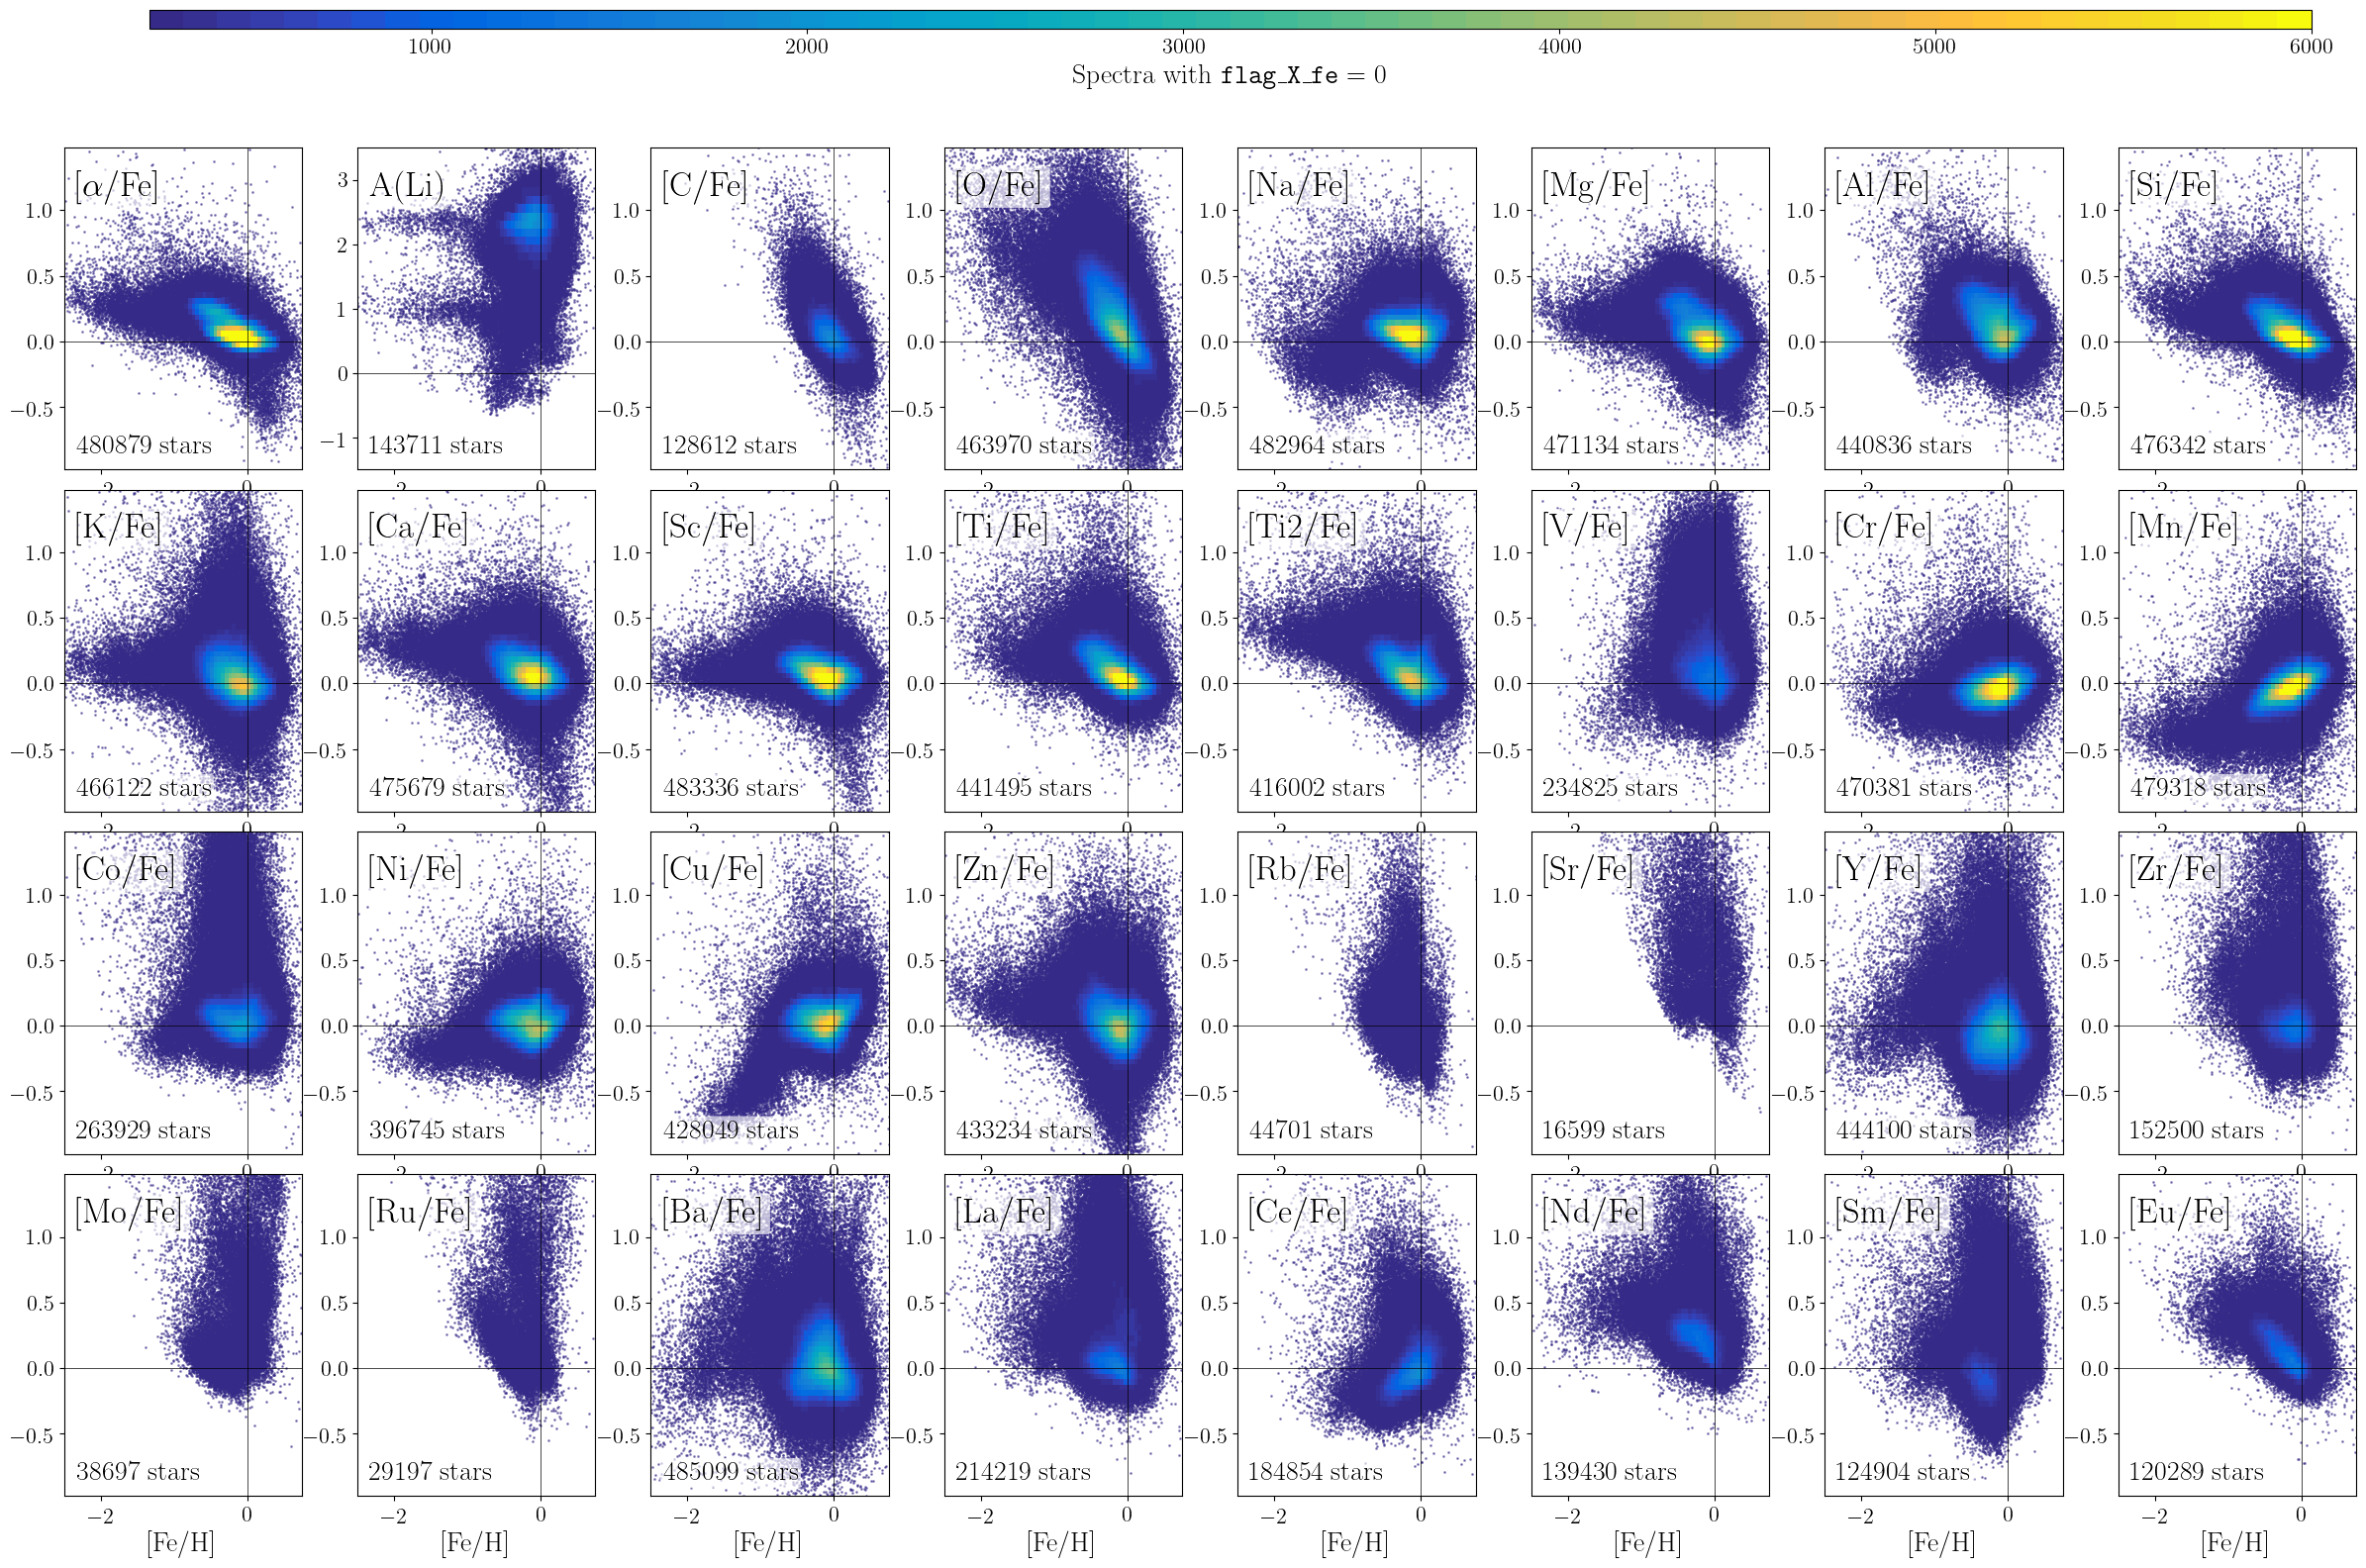
\includegraphics[width=\columnwidth]{Figures/dr3_abundance_overview_31_elements.png}
\caption{Distribution of the element abundances included in GALAH Data Release 3 over the iron abundance [Fe/H]. Shown are relative abundances [X/Fe] for stars with $\texttt{X\_FE\_FLAG} = 0$ (with exception of Li, for which we show the absolute abundance). Colours indicate the stellar density, truncated at a maximum of 6000 per density bin.} 
\label{fig:abundance_overview}
\end{figure}
\end{landscape}

\begin{figure*}
  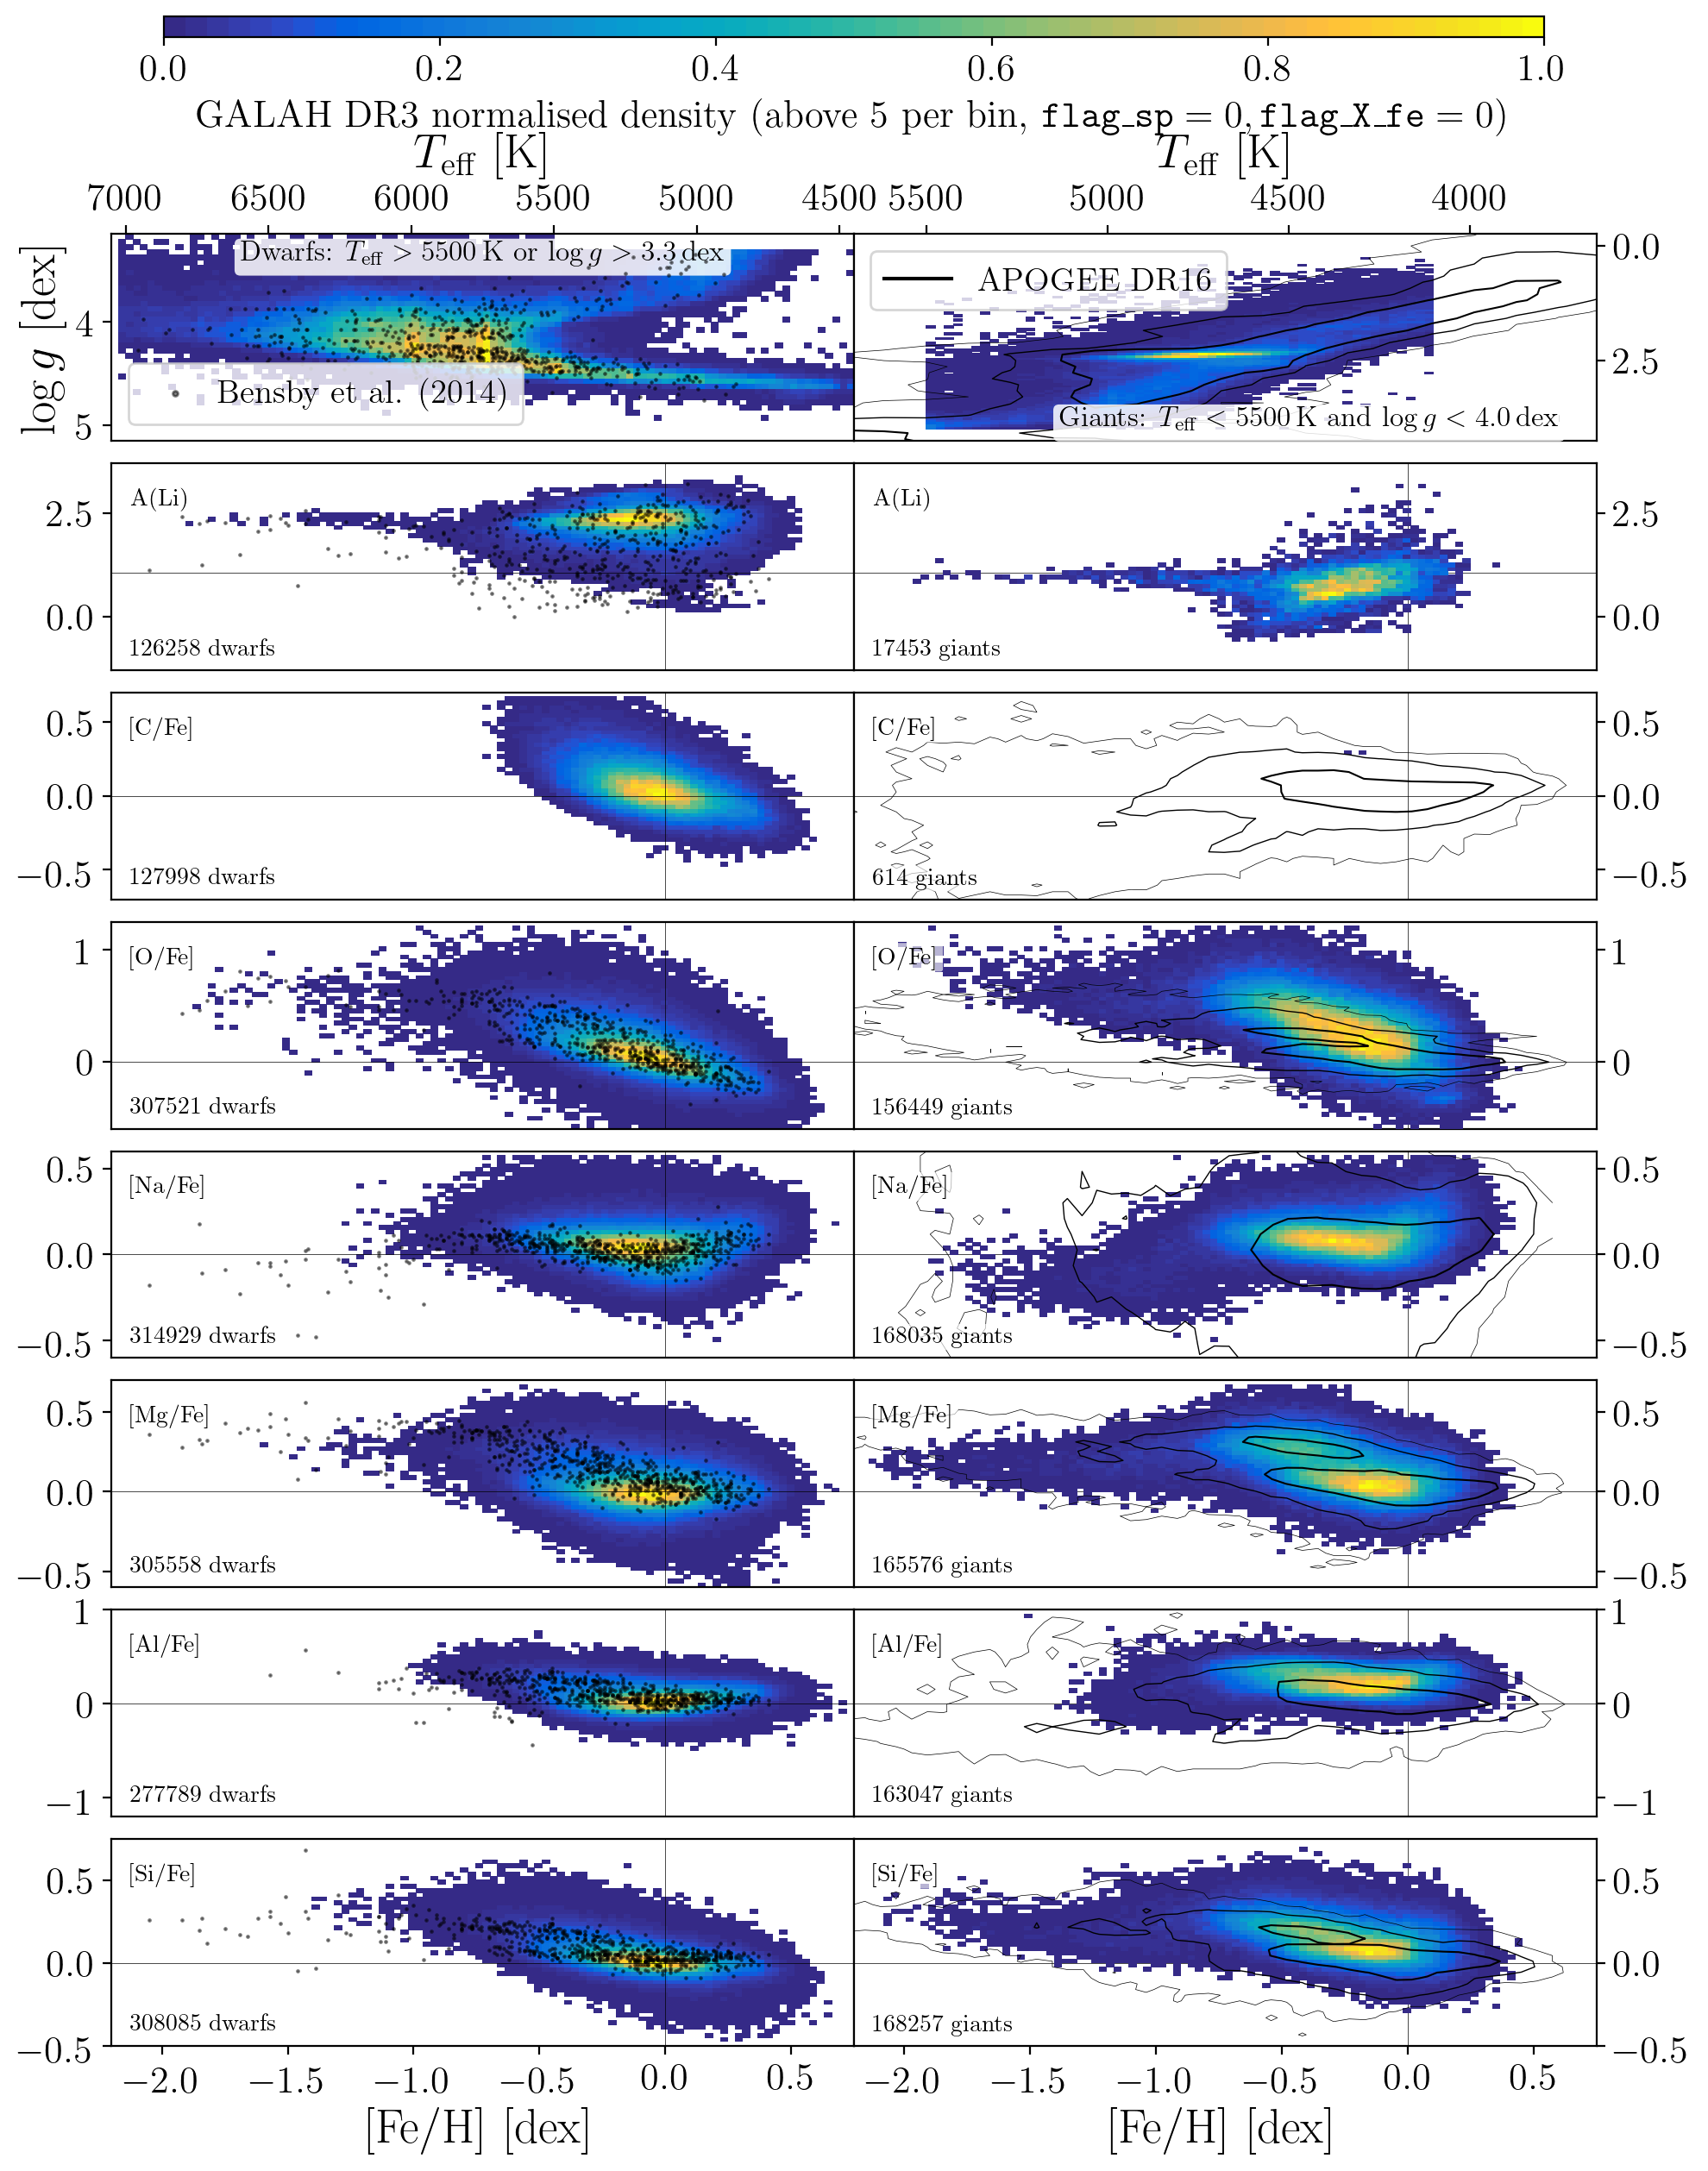
\includegraphics[width=0.975\textwidth]{Figures/Dwarf_Giant_comparison1_flag0.png}
\caption{Comparison of individual abundances with the sample of 714 dwarfs \citep{Bensby2014, Battistini2015, Battistini2016, Bensby2018} on the left hand side as well as APOGEE DR16 giants \citep{SDSSDR16} on the right hand side. GALAH DR3 data (with $\texttt{flag\_sp} = 0$ for stellar parameters and $\texttt{flag\_X\_fe} = 0$ for the respective element X) are plotted as colored density with a minimum of 5 stars per bin. The literature values for dwarfs are overplotted as black dots, while the APOGEE giants (with finite values, $\texttt{ASPCAPFLAG} = 0$, and $\texttt{STARFLAG} = 0$ for stellar parameters as well as $\texttt{X\_FE\_FLAG} = 0$ for the respective element X).}
  \label{fig:Dwarf_Giant_comparison1_flag0}
\end{figure*}

\begin{figure*}
  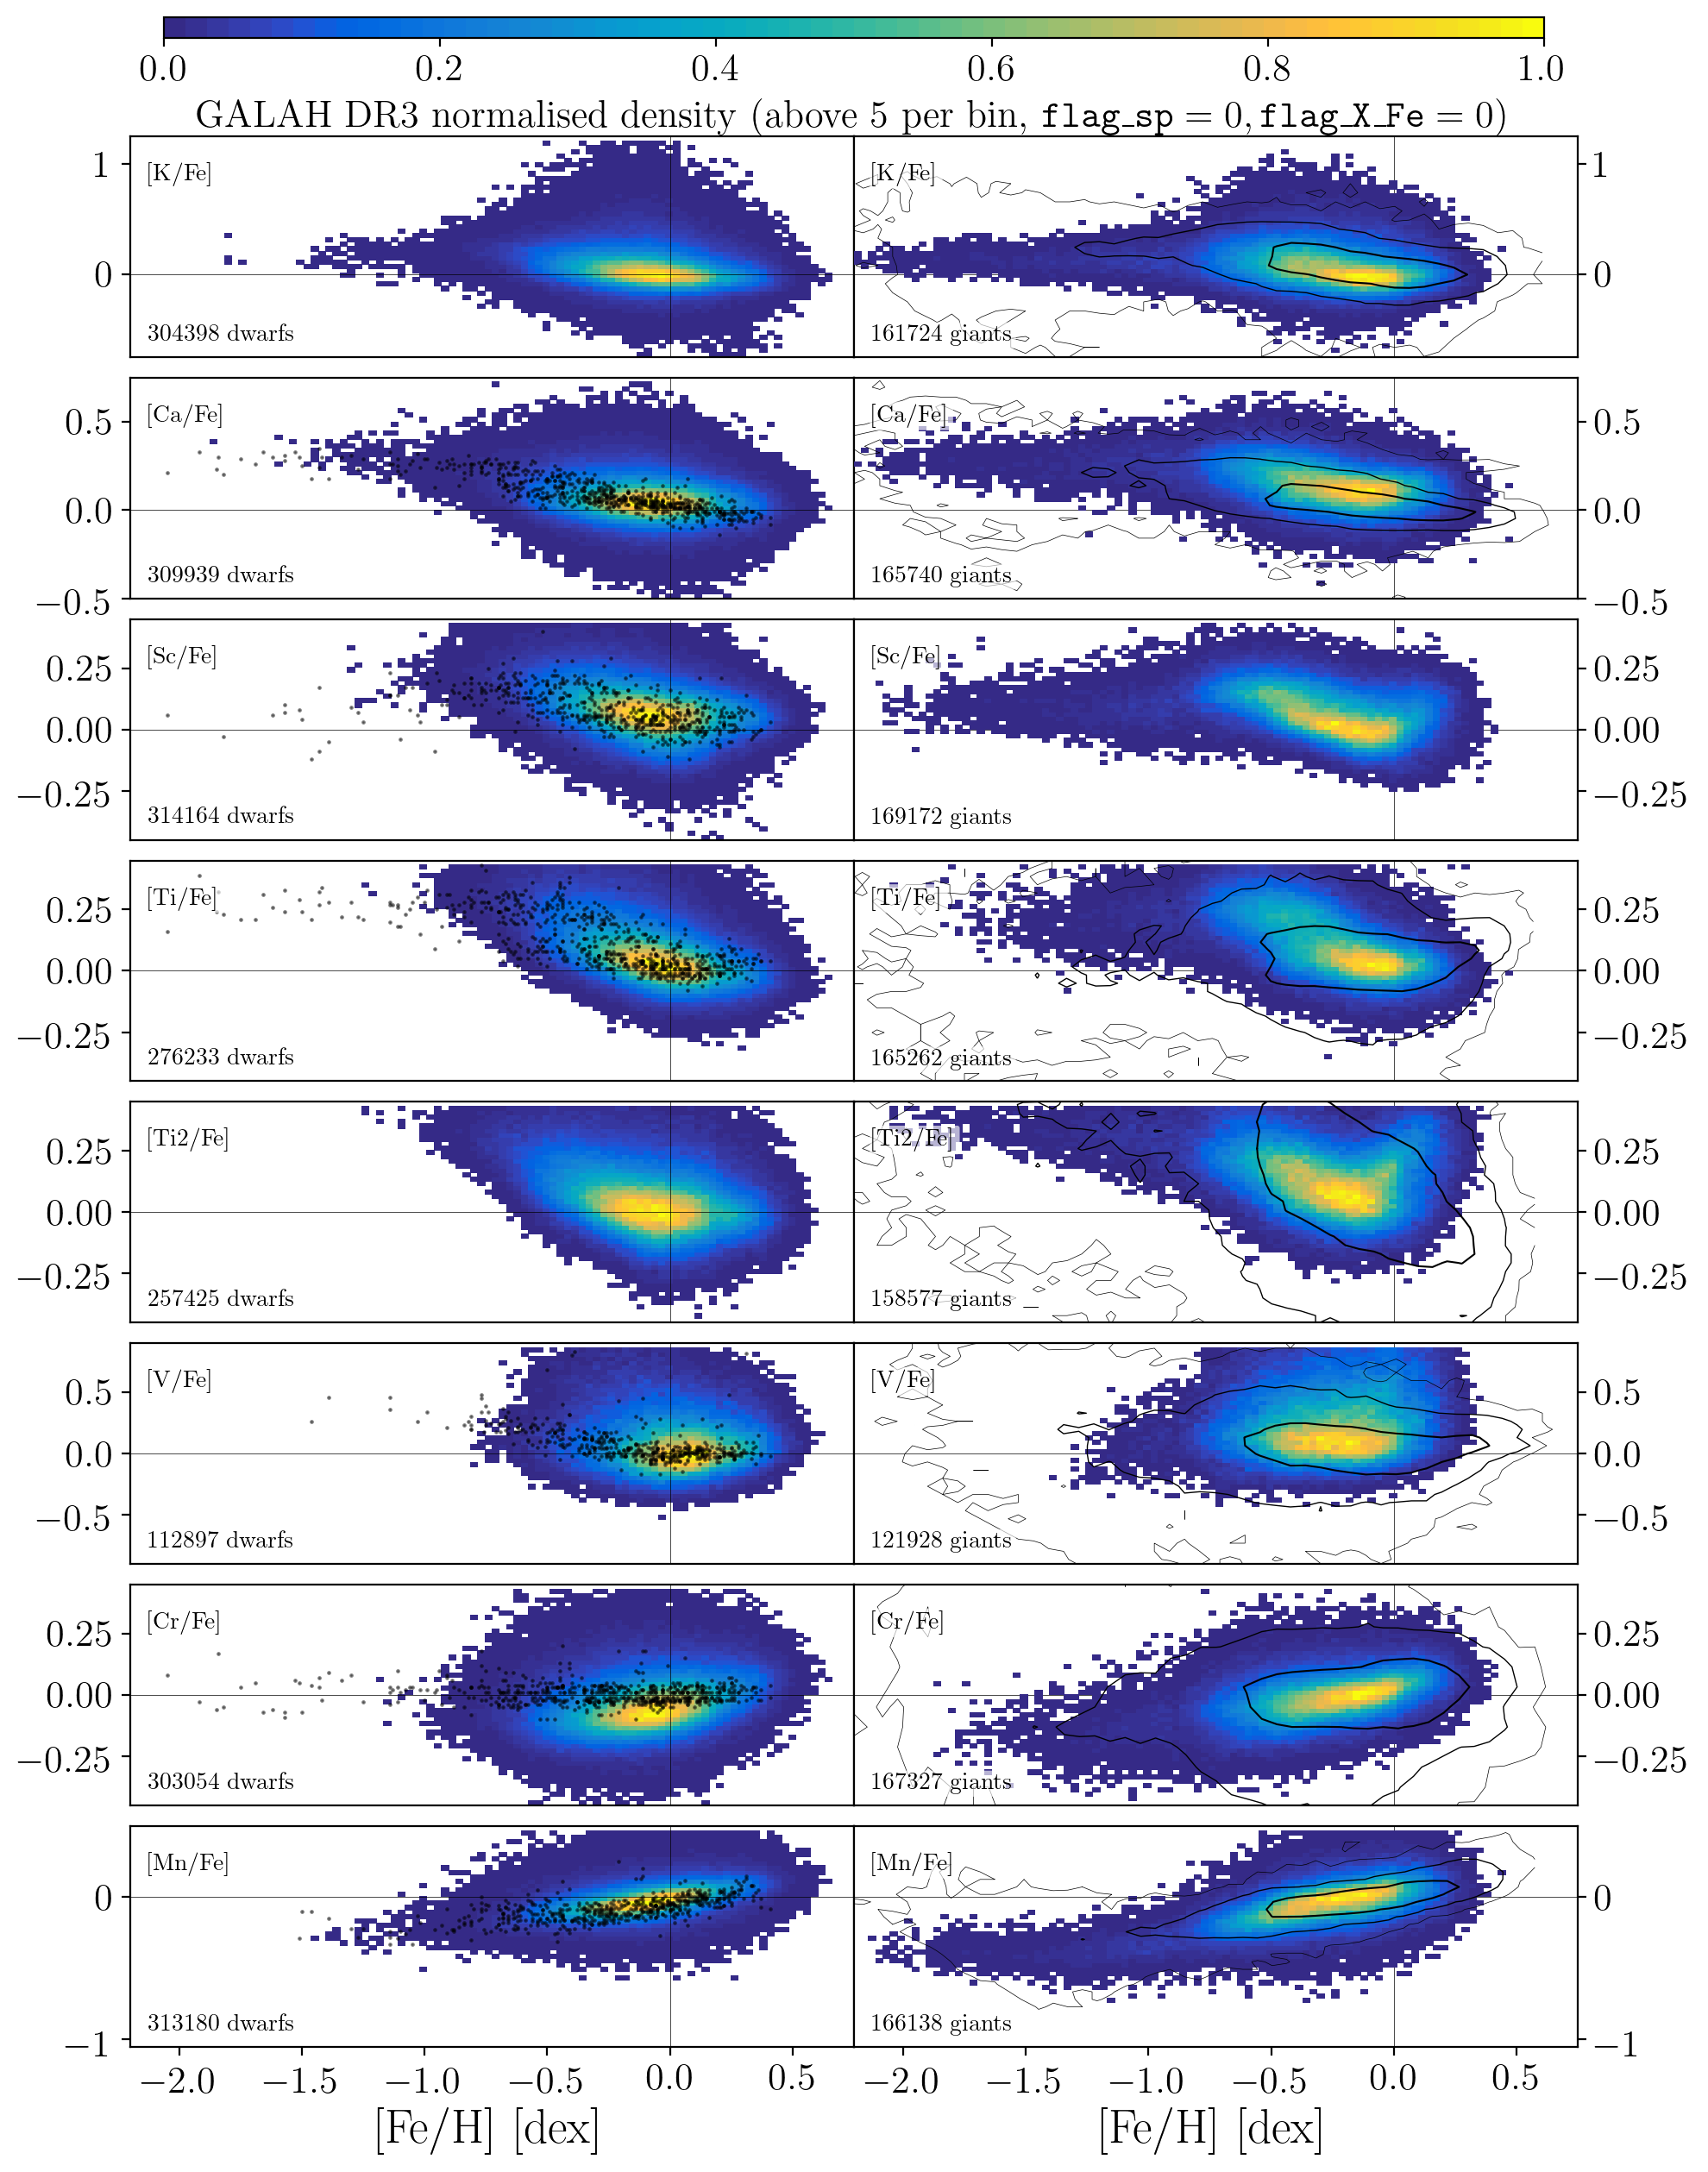
\includegraphics[width=0.975\textwidth]{Figures/Dwarf_Giant_comparison2_flag0.png}
\caption{Continuation of Fig.~\ref{fig:Dwarf_Giant_comparison1_flag0} for elements K through Mn.}
  \label{fig:Dwarf_Giant_comparison2_flag0}
\end{figure*}

\begin{figure*}
  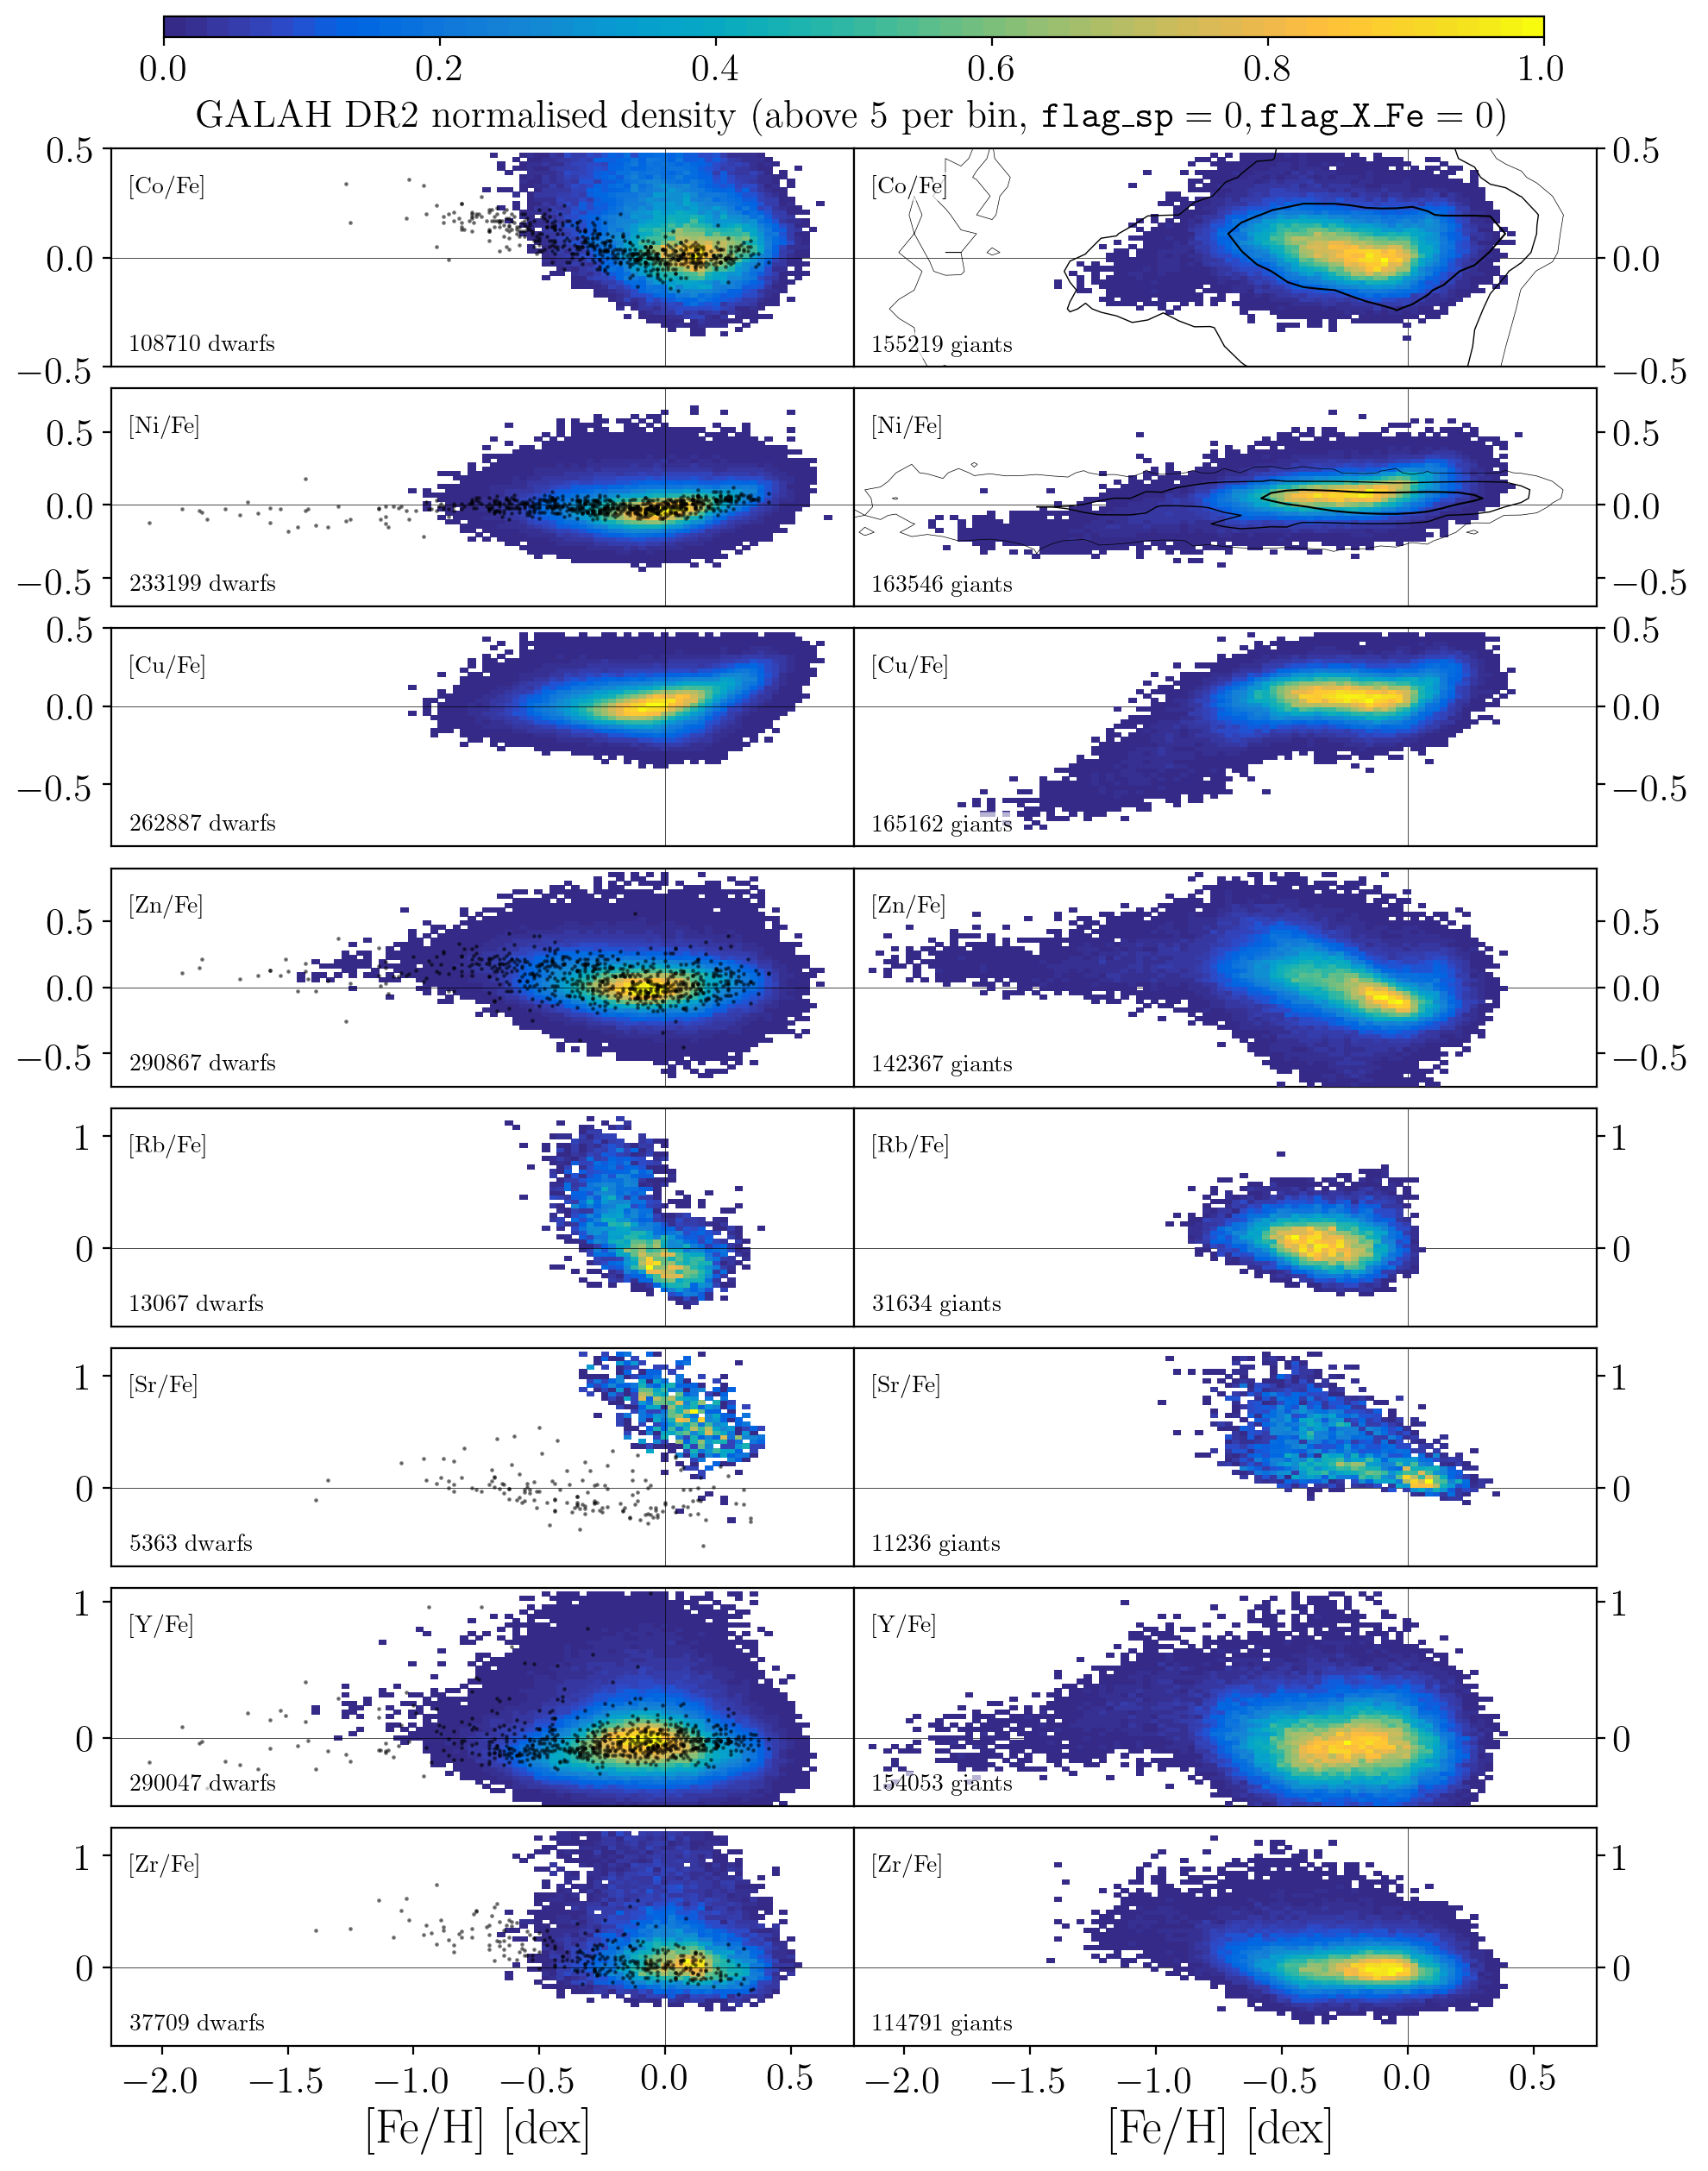
\includegraphics[width=0.975\textwidth]{Figures/Dwarf_Giant_comparison3_flag0.png}
\caption{Continuation of Figs.~\ref{fig:Dwarf_Giant_comparison1_flag0} and \ref{fig:Dwarf_Giant_comparison2_flag0} for elements Co through Zr.}
  \label{fig:Dwarf_Giant_comparison3_flag0}
\end{figure*}

\begin{figure*}
  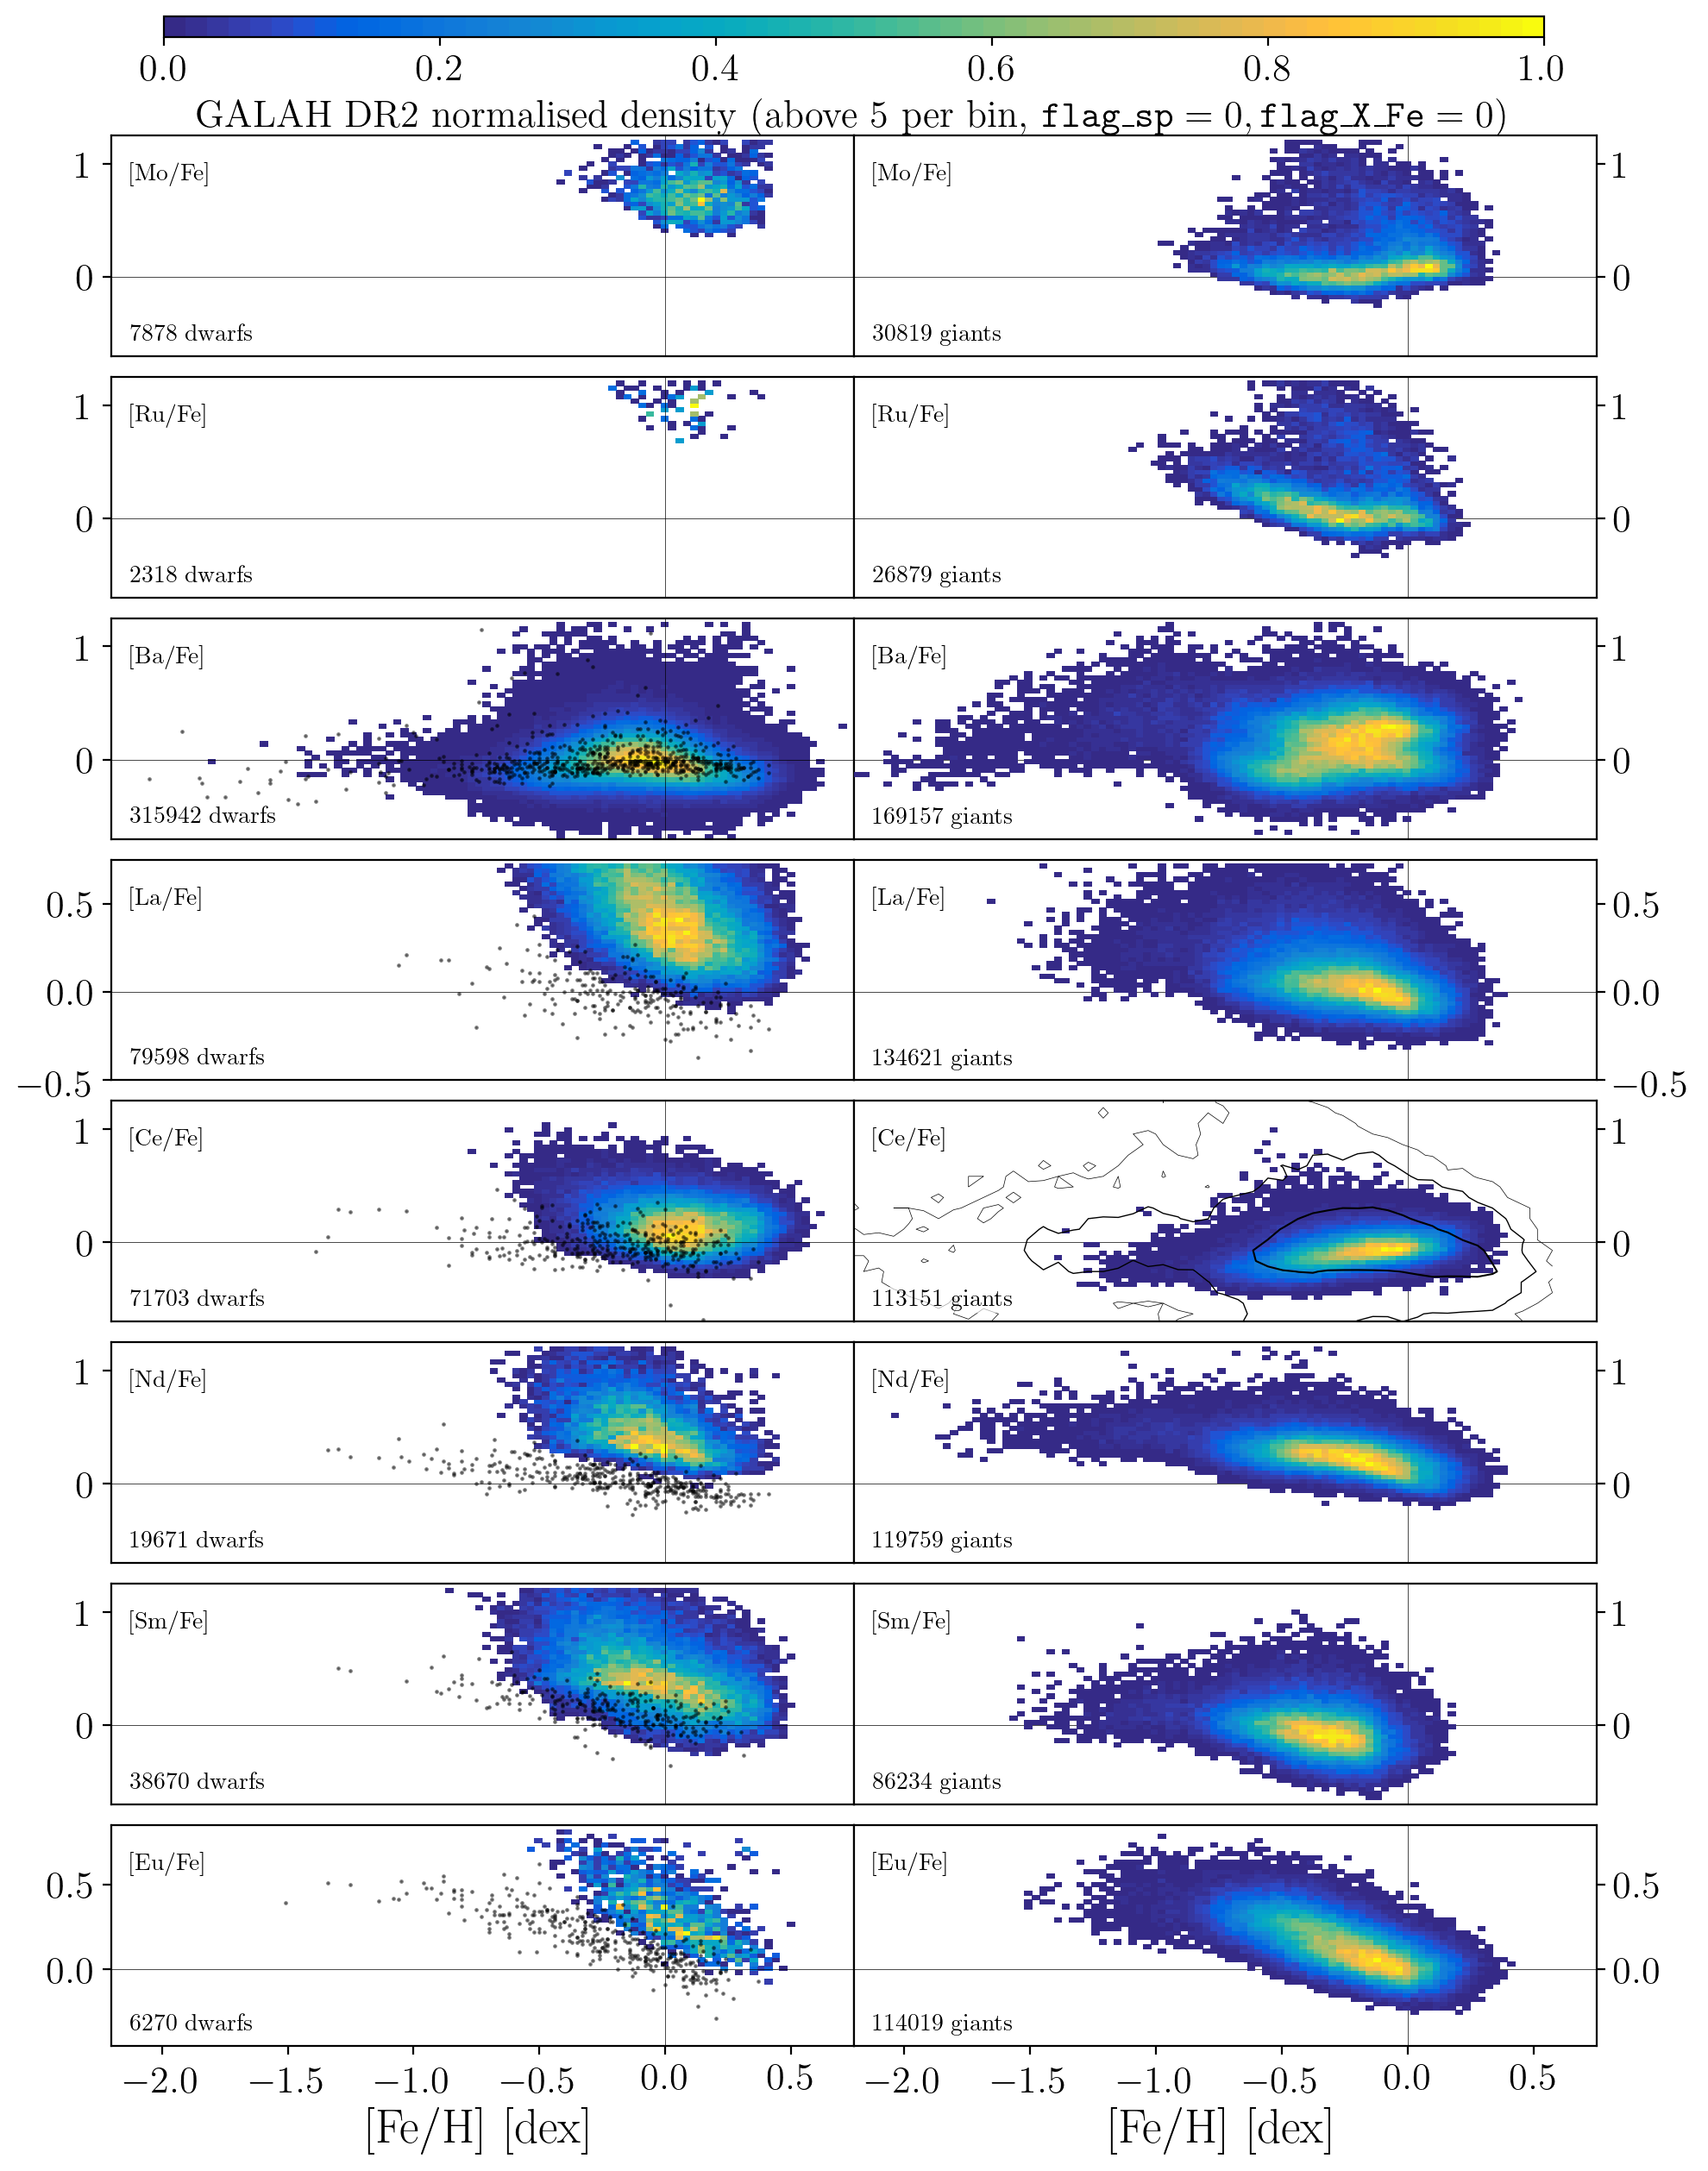
\includegraphics[width=0.975\textwidth]{Figures/Dwarf_Giant_comparison4_flag0.png}
\caption{Continuation of Figs.~\ref{fig:Dwarf_Giant_comparison1_flag0} to \ref{fig:Dwarf_Giant_comparison3_flag0} for elements Mo through Eu.}   \label{fig:Dwarf_Giant_comparison4_flag0}
\end{figure*}

%________________________________________________________________
\subsection{Value-Added-Catalogs (VACs)} \label{sec:value_added_catalogs}

The third Data Release of GALAH is accompanied by two value-added-catalogs and we explain them in this section. One value-added-catalog includes extended abundance measurement information, another one stellar ages as well as masses and a third one kinematic as well as dynamic information for each star.

\subsubsection{Extended abundance measurement information}

This VAC includes:
\begin{enumerate}
\item A(X) for each line of an element
\item Precision uncertainties for each abundance
\item flag for each line of an element
\item line flux estimates for each line of an element
\end{enumerate}

\subsubsection{Stellar age and mass estimates} \label{sec:vac_age}

As part of the stellar parameter estimation (see Secs.~\ref{sec:analysis}), both stellar masses and ages have been estimated and are added to the data release in a value-added-catalog. In Fig.~\ref{fig:mass_age_sanders}, we compare the mass and age difference to the study by \citet{Sanders2018}, who estimated both values based on GALAH DR2   as well as \Gaia DR2 in a Bayesian framework. We only compare those 215493 stars with \texttt{flag\_sp=0} from GALAH DR3 and  \texttt{flag=0} as well as \texttt{log10\_age>-1} (expected binaries) from \citet{Sanders2018} and find a good agreement between both analyses. For the masses we find an agreement in $\log_{10} (M)$ within 0.1 for 95\% of the stars and even within 0.05 for 82\% of the stars. The largest deviations are found both for massive stars (where GALAH masses are higher) and the metal-rich RC stars (where GALAH masses are lower). Regarding stellar ages we find a generally good agreement as well, with 73\% of the ages agreeing within 30\%. We note however, that especially for the young main-sequence and secondary RC stars  (on the GALAH scale), \citet{Sanders2018} tend to estimate even lower ages, whereas they estimate higher ages for cool main-sequence and metal-rich RC stars than our algorithm. Both regimes are prone to systematic trends, because the isochrone grids are very dense, that is tracks for very different masses and metallicities are very close.

\begin{figure*}
\centering
\includegraphics[width=0.49\textwidth]{figures/old/DS18_mass.pdf}
\includegraphics[width=0.49\textwidth]{figures/old/DS18_age.pdf}
  \caption[{Comparison of mass (left) and age (right) estimates from GALAH DR3 and \citet{Sanders2018}.}]{Comparison of mass (left) and age (right) estimates from GALAH DR3 and \citet{Sanders2018}.}
  \label{fig:mass_age_sanders}
\end{figure*}

We have further tested how well our algorithm can reproduce stellar ages from mock data, by selecting isochrone points of the 4 stellar ages (4.5, 8.0, 10.0, and $13.5\,\mathrm{Gyr}$), 4 different iron abundances ($\mathrm{[Fe/H]} \in [-2.0,-1.1,-.07,0.0]$), and 5 evolutionary stages, that is main-sequence ($T_\text{eff} \sim 5250\,\mathrm{K}$), turn-off (hottest around $\log g \sim 4.1$), RGB ($\log g \sim 3.25$), tip of the RGB ($\log g \sim 1.0$), and core helium burning RC (hottest for $2.0 < \log g < 3.0$). Each mock star is fed into the the mass and age estimation algorithm with generic uncertainties for the input parameters of $\Delta T_\text{eff} = 100\,\mathrm{K}$, $\Delta \log g = 0.5$, $\Delta \mathrm{[Fe/H]} = 0.2$, and $\Delta L_\text{bol} = 10\%$. We compare the retrieved age with the input age in Fig.~\ref{fig:Age_deviation_trends} and find that the age estimation tends to recover the stellar ages very well for turn-off stars as well as intermediate age stars around $8-10\,\mathrm{Gyr}$. For younger stars, the code tends to overestimate the age by up to $75\%$ for main-sequence stars and those at the tip of the RGB. The age of the oldest is typically underestimated, but RC and RGB star ages are better recovered than those of the tip of the RGB and the main-sequence. This means that the age of the oldest stars are typically underestimated and those of the youngest stars overestimated, resulting in an artificially tighter age distribution towards intermediate age stars. The code can, however, identify truly young stars and truly old stars.

\begin{figure*}
\centering
\includegraphics[width=\textwidth]{figures/old/Age_deviation_trends_rel.pdf}
  \caption[{Relative deviation of estimated stellar age from stellar ages as chosen from isochrone points.}]{Relative deviation of estimated stellar age from stellar ages as chosen from isochrone points at different $\mathrm{[Fe/H]} \in [-2.0, -1.1, -.07, 0.0]$ (as indicated in lower right of each panel), different stellar $\mathrm{ages} \in [4.5, 8.0, 10.0, 13.5]\,\mathrm{Gyr}$ (different bars with same colours as indicated by axis labels) and different evolutionary stages (different colours as indicated by plot legend in upper left panel).}
  \label{fig:Age_deviation_trends}
\end{figure*}

\subsubsection{Kinematic and dynamic information}

We provide a value-added-catalog with kinematic and dynamic information, that builds upon the 5D astrometric information by \Gaia DR2 and radial velocities preferably from GALAH DR3 and otherwise from \Gaia DR2. Where possible, we use more reliable distances, preferably those estimated via isochrone matching as part of the BSTEP grid-based modelling (see description in Sec.~\ref{sec:vac_age}), otherwise we use the prior-informed values by \citet{BailerJones2018}.

For the calculation of orbit information we use version 1.6 of the python package {\sc galpy} \citep{Bovy2015}. More specifically, we use its {\sc orbit} module for coordinate/velocity transformation as well as orbit energy computation. To estimate actions, eccentricity, maximum orbit Galactocentric height, and apocenter/pericenter radii, we use the Staeckel fudge via the {\sc galpy} module {\sc actionAngleStaeckel} with a focus of 0.45.

For our calculations we use the best fitting axisymmetric potential by \citet{McMillan2017} with a solar radius of $8.21\,\mathrm{kpc}$, consistent with the latest measurement by \citet{Abuter2019} of $8.178 \pm 0.013_\text{stat.} \pm 0.022_\text{sys.}\,\mathrm{kpc}$, and circular velocity at this radius of $233.1\,\mathrm{km\,s^{-1}}$. We use the total motion of the Sun in V-direction of $248.27\,\mathrm{km\,s^{-1}}$ by evaluation the proper motion measurements from \citet{Reid2004} at our chosen Solar radius. We further place the Sun $25\,\mathrm{pc}$ above the plane \citep{Juric2008} and use the peculiar solar velocities $U_\odot = 11.1_{-0.75}^{+0.69}\,\mathrm{km\,s^{-1}}$ and $7.25_{-0.36}^{+0.37}\,\mathrm{km\,s^{-1}}$ by \citet{Schoenrich2010}, but $V_\odot = 15.17\,\mathrm{km\,s^{-1}}$ (contrary to their value of $12.24_{-0.47}^{+0.47}\,\mathrm{km\,s^{-1}}$ for consistency between the chosen total and peculiar motions of the Sun in our reference frame. 

For the Sun, this leads actions of $J_R = 7.7\,\mathrm{kpc\,km\,s^{-1}}$, $J_\phi = L_Z = 2038.3\,\mathrm{kpc\,km\,s^{-1}}$, and $J_Z = 0.4\,\mathrm{kpc\,km\,s^{-1}}$ on an orbit with eccentricity 0.073, a pericenter radius of $8.15\,\mathrm{kpc}$, apocenter radius of $9.43\,\mathrm{kpc}$ and a total energy of $E_{n,\odot} = -1.53\cdot 10^5\,\mathrm{km^2\,s^{-2}}$.

We provide columns for the heliocentric cartesian coordinate ($X$, $Y$, $Z$) and velocity frames ($U$, $V$, $W$) as well as the Galactocentric cylindrical coordinate ($R$, $\phi$, $z$) and velocity frames ($v_R$, $v_\phi$ as well as $v_T$, $v_z$) together with the actions ($J_R$, $J_\phi = L_Z$, $J_Z$), eccentricity ($e$), maximum Galactocentric orbit height ($z_\text{max}$), pericenter and apocenter radii ($R_\text{peri}$, $R_\text{ap}$), as well as orbit energies for the best value input. We further realise 10,000 Monte Carlo samplings per star/spectrum by sampling \Gaia astrometry within the uncertainties\footnote{When using more elaborate distance estimates, we neglect the covariances, but also provide the possibility to sample distances from parallaxes while taking \Gaia covariances into account.}. For the distance sampling, we assume Gaussian uncertainties when using the BSTEP distances or sample from a 2-sided Gaussian based on the bold assumption that the distributions left and right of the mode stated by \citet{BailerJones2018} are Gaussian and we can thus describe them via the stated lower and higher percentiles\footnote{We want to stress however, that given the excellent parallax quality for the vast majority of our sample (see Fig.~\ref{fig:distance}), these choices are only affecting a very small number of typically very distant stars with uncertain parallaxes, for which we caution the user to carefully assess the quality of both the astrometry as well as our distance and thus kinematic/dynamic estimates.}. We then provide the 5th, 50th, and 95th percentile for the user for each orbit parameter.

The distribution in Galactocentric cylindrical coordinates ($R,z$) is shown in panel a) and a top view ($X,Y$) in Fig.~\ref{fig:dr3_apogee_lamost}. The vast majority of targets are distributed within less than $4\,\mathrm{kpc}$ from the Sun and covers a large fraction of the disk. The distribution shows an asymmetry along $R$ as well as in the $(X,Y)$ plane due fact that the observations are carried out from Australia. Because of the target selection of the GALAH main program ($\vert b \vert > 10\,\mathrm{deg}$), no stars are observed close to the Galactic plane. We note, however, that GALAH DR3 includes also observations from TESS-HERMES, K2-HERMES, and several smaller projects that targeted the Galactic bulge and clusters. The distribution in the panel a) is hence also including observations with $\vert b \vert < 10\,\mathrm{deg}$ especially towards the Galactic center at ($R,z$) = 0. A combination of distance uncertainties and special targeting of clusters and K2/TESS fields is causing finger-of-god effects in both panels.

The space velocities $(U,V,W)$ in the Galactocentric cartesian coordinate frame are shown in a Toomre diagram in panel a) of Fig.~\ref{fig:DR3_dynamics_overview}. Most of the stars observed as part of GALAH DR3 have disk-like kinematics similar to the local standard of rest, but an extension of stars with lower rotational velocity than the disk ($V \ll 0\,\mathrm{km\,s^{-1}}$) are shown and indicate that also several stars with halo-like kinematic properties are part of GALAH DR3.

We compute stellar dynamic properties, that is actions $J_R, L_z, J_z$, eccentricities $e$, and orbit boundary information such as $z_\text{max}$, $R_\text{peri}$, and $R_\text{apo}$ with {\sc galpy} \citep{Bovy2015} in the {\sc MWPotential2014} and a Staeckel fudge with 0.45 as focal length of confocal coordinate system.

The distribution of stars in action space is shown in a view of vertical angular momentum (normalised to the Solar value) and radial action in panel b) of Fig.~\ref{fig:DR3_dynamics_overview}. Most of the stars in this diagram show a similar vertical angular momentum radial action as the Sun. Similar to the analyses by \citet{Trick2019}, a rich substructure along $J_R$ can be seen. Similar to the extensions seen in the left panel of that figure, an extension of stars with lower vertical angular momentum is visible. We also note an overdensity close to $(L_Z,J_R) = (0,0)\,\mathrm{kpc\,km\,s^{-1}}$, that is an overdensity of stars with near-circular orbits close to the Galactic center and bulge. The overdensity of stars around $L_Z \sim 0 \,\mathrm{kpc\,km\,s^{-1}}$ with higher radial actions is typical for stars of the Galactic halo and is assessed in Chapter~\ref{sec:halo}.

For each of the computed phase space and dynamic properties, we report a variety of statistical values. In addition to the best-value, that is computed by using the best values as input, we also sample the distribution for each property within the uncertainties via Monte Carlo sampling with size 10000 and report the 5th, 50th, and 95th percentiles of these distributions. An example of the sampling of parameters for 100 randomly selected stars is shown in Fig.~\ref{fig:MC_output}.  We also provide the code to perform this sampling with different sampling choices. Whereas we currently sample the properties by assuming their input parameters are uncorrelated, we also provide the code to sample with the \Gaia correlation matrices. The latter are currently not applying a distance prior and are thus problematic for large distances. However, we stress, that the vast majority of the stars from GALAH DR3 have very precise parallax measurements, for which the sampling choice is negligible (see Fig.~\ref{fig:parallax_overview}).

\begin{figure*}
\centering
\includegraphics[width=\textwidth]{figures/old/MC_output.pdf}
  \caption[{Overview of phase space and dynamic stellar properties for randomly chosen stars from GALAH DR3, including their sampling within the measurement uncertainties.}]{Overview of phase space and dynamic stellar properties for randomly chosen stars from GALAH DR3, including their sampling within the measurement uncertainties. The black points indicate the values calculated from the best 6D information. Blue points indicate 10000 samples from the 6D information per star within the uncertainties. Red error bars indicate the distribution between 50th percentile (middle of the cross) and the 5th and 95th percentile, respectively.}
  \label{fig:MC_output}
\end{figure*}

\subsubsection{Double-lined spectroscopic binary stars}

Binary stellar systems represent a significant fraction of stars in our Galaxy. Therefore, their effect on observations, as well as their impact on the Galactic environment, have to be properly taken into account when studying Galactic structure and evolution. To this end, we present a sample of 12\,760 binary systems for which the properties of their stellar components were derived in a separate analysis from the one described in Sec.~\ref{sec:analysis}. In order to compute individual parameters for both stars ($T_{\rm eff[1,2]}$, $\log g_{[1,2]}$, $V_{r[1,2]}$, $v_{\rm mic[1,2]}$, $v_{\rm broad[1,2]}$, $R_{[1,2]}$), together with a common metallicity and extinction for the binary system which they form ([Fe/H], $E(B-V)$), we combine information from GALAH spectra, Gaia DR2 parallax, and data from several photometric surveys (APASS; \citealt{APASS}, \textit{Gaia} DR2; \citealt{Brown2018}, 2MASS; \citealt{Skrutskie2006}, WISE; \citealt{Cutri2013}) into a joint Bayesian scheme. The details of the analysis are described in \citet{Traven2020}, and the catalogue of derived parameters is available at CDS\footnote{\url{http://cdsarc.u-strasbg.fr/viz-bin/cat/J/A+A/638/A145}}. 

The binary stars presented in this VAC were detected in a sample of 587\,153 spectra from the second GALAH internal data release. We investigated direct products of the reduction pipeline before implementation of some improvements described in Sec.~\ref{sec:reductions}. Detection of binarity was performed using a t-SNE classification and a cross-correlation analysis \citep{Merle2017, Traven2017} of GALAH spectra. The final sample of this catalogue consists of systems with mostly dwarf components, a significant fraction of evolved stars, and also several dozen members of the giant branch.  The statistical distributions of derived stellar properties can be further used for population studies (Traven et al., in prep), and show trends which are expected for a population of close binary stars ($a < 10$ AU) with mass ratios $0.5 \leq q \leq 1$. Our results additionally indicate that the derived metallicity of binary stars is statistically lower than that of single dwarf stars observed in the same magnitude-limited sample of the GALAH survey.

%________________________________________________________________
\section{GALAH DR3 in context} \label{sec:galah_in_context}

\subsection{Galactic archaeology on a global scale}  \label{sec:global_ga}

\begin{figure*}
\centering
\includegraphics[width=\textwidth]{figures/GALAHDR3_APOGEEDR16_LAMOSTDR5VAC.png}
  \caption{Comparison of GALAH DR3 (left panels) with APOGEE DR16 (middle panels) and LAMOST DR5 VAC (right panels). The surveys trace different stellar types (seen in the top panels with an overview of the \Teff-\logg coverage) across different Galactic regions (second and third row showing coverages for different coordinate systems), and different stellar populations (shown in the [Fe/H] vs. [$\upalpha$/Fe] diagram in the bottom row.}
  \label{fig:dr3_apogee_lamost}
\end{figure*}

\begin{figure*}
\centering
\includegraphics[width=\textwidth]{figures/RZ_alpha.png}
  \caption{Coverage of element abundances [Fe/H] vs. [$\upalpha$/Fe] measured by GALAH for different spatial regions ($R$,$z$) of the Galaxy. Compare to \citet{Hayden2015}.}
  \label{fig:RZ_alpha}
\end{figure*}

\begin{figure*}
\centering
\includegraphics[width=\textwidth]{figures/DR3_dynamics_overview.png}
  \caption{Coverage of stellar kinematics (space velocities) and dynamics (actions) for the stars observed as part of GALAH. Panel a) shows a Toomre diagram\citep[compare to e.g.][]{Bonaca2017}, panel b) two actions \citep[compare to e.g.][]{Trick2019}, panel c) Galactic space velocities \citep[compare to e.g.][]{Belokurov2018}, and panel d) the distribution of actions \citep[compare to e.g.][]{Vasiliev2019}.}
  \label{fig:DR3_dynamics_overview}
\end{figure*}

\subsection{Chemodynamical evolution}  \label{sec:cde}

Combining chemistry, dynamics, and ages of stars

I have added 4 panels in Fig.~\ref{fig:DR3_dynamics_overview}:
\begin{itemize}
\item plot Galactic $v_R$ vs. $v_\phi$ (Belokurov)
\item plot Toomre diagram
\item plot actions
\item plot \cite{Vasiliev2019} overview of $J_i$
\end{itemize}

\begin{figure*}
\centering
\includegraphics[width=\textwidth]{figures/DR3_action_xfe.png}
  \caption{Overview of actions, colored by mean [Fe/H] (panel a), and mean [$\upalpha$/Fe] (panel b).}
  \label{fig:DR3_action_xfe}
\end{figure*}

\paragraph*{Lithium}

\citet{Cescutti2020} Lithium in Gaia-Enceladus: \url{http://arxiv.org/abs/2004.06606v1}

\begin{figure*}
\centering
\includegraphics[width=\textwidth]{figures/DR3_Li_overview.png}
  \caption{Coverage of stellar types for stars with different amounts of Li abundances, panel a) $3.0 < \mathrm{A(Li)}$, panel b) $2.2 < \mathrm{A(Li)} \leq 3.0$, panel c) $\mathrm{A(Li)} \leq 2.2$}
  \label{fig:DR3_Li_overview}
\end{figure*}



%________________________________________________________________
\section{Conclusions} \label{sec:conclusions}


%________________________________________________________________
\section*{Acknowledgements}

Based on data acquired through the Australian Astronomical Observatory, under programmes: A/2013B/13 (The GALAH pilot survey); A/2014A/25, A/2015A/19, A2017A/18 (The GALAH survey phase 1), A2018 A/18 (Open clusters with HERMES), A2019A/1 (Hierarchical star formation in Ori OB1),  A2019A/15 (The GALAH survey phase 2), A/2015B/19, A/2016A/22, A/2016B/10, A/2017B/16, A/2018B/15 (The HERMES-TESS program), and A/2015A/3, A/2015B/1, A/2015B/19, A/2016A/22, A/2016B/12, A/2017A/14, (The HERMES K2-follow-up program). \SB{Are we missing programs?} We acknowledge the traditional owners of the land on which the AAT stands, the Gamilaraay people, and pay our respects to elders past and present.

This work has made use of data from the European Space Agency (ESA) mission \Gaia (http://www.cosmos.esa.int/gaia), processed by the \Gaia Data Processing and Analysis Consortium (DPAC, http://www.cosmos.esa.int/web/gaia/dpac/consortium). Funding for the DPAC has been provided by national institutions, in particular the institutions participating in the \Gaia Multilateral Agreement. 

This publication makes use of data products from the Two Micron All Sky Survey, which is a joint project of the University of Massachusetts and the Infrared Processing and Analysis Center/California Institute of Technology, funded by the National Aeronautics and Space Administration and the National Science Foundation.

The following software and programming languages made this research possible: \textsc{IRAF} \citep{Tody1986,Tody1993}, \textsc{configure} \citep{Miszalski2006}, \textsc{topcat} \citep[version 4.4;][]{Taylor2005}; Python (version 3.7) and its packages {\textsc{astropy}} \citep[version 2.0;][]{Robitaille2013,PriceWhelan2018}, {\textsc{scipy}} \citep{scipy}, {\textsc{matplotlib}} \citep{matplotlib}, {\textsc{pandas}} \citep[version 0.20.2;][]{McKinney2011}, {\textsc{NumPy}} \citep{numpy}, {\textsc{IPython}} \citep{ipython}, and  \textsc{galpy} \citep[version 1.3;][]{Bovy2015}. This research has made use of the VizieR catalogue access tool, CDS, Strasbourg, France. The original description of the VizieR service was published in A\&AS 143, 23. This research mad use of the TOPCAT tool, described in \citet{Taylor2005}. This publication makes use of data products from the Two Micron All Sky Survey, which is a joint project of the University of Massachusetts and the Infrared Processing and Analysis Center/California Institute of Technology, funded by the National Aeronautics and Space Administration and the National Science Foundation.

SB and acknowledges funds from the Alexander von Humboldt Foundation in the framework of the Sofja Kovalevskaja Award endowed by the Federal Ministry of Education and Research. SB acknowledges travel support from Universities Australia and Deutsche Akademische Austauschdienst. DMN acknowledges support from NASA under award Number 80NSSC19K0589, and support from the  Allan C. And Dorothy H. Davis Fellowship. YST is supported by the NASA Hubble Fellowship grant HST-HF2-51425 awarded by the Space Telescope Science Institute.

We thank Jane Lin for providing an early version of the {\sc elli} code \citep{Lin2018} of which the initial likelihood optimisation part was implemented in an adjusted form (e.g. different isochrones) for the analysis of this data release.
We would like to thank Chris Onken for crossmatching GALAH and SkyMapper DR3 data. \SB{Put SkyMapper REF here or up in the main text}
We thank Kareem El-Badry for providing a vetted version of wide binaries from the 5-dimensional \Gaia DR2 data and GALAH DR3 radial velocities.
We would like to thank the SDSS collaboration and APOGEE team for their efforts in documentation, which greatly benefited our efforts in documentation and validation.

%%%%%%%%%%%%%%%%%%%%%%%%%%%%%%%%%%%%%%%%%%%%%%%%%%

%%%%%%%%%%%%%%%%%%%% REFERENCES %%%%%%%%%%%%%%%%%%

% The best way to enter references is to use BibTeX:

\bibliographystyle{mnras}
\bibliography{bib} % if your bibtex file is called example.bib

%%%%%%%%%%%%%%%%%%%%%%%%%%%%%%%%%%%%%%%%%%%%%%%%%%

\newpage
\noindent \rule{8.5cm}{1pt}

\noindent
% List of institutions
$^{1}$Max Planck Institute  for Astronomy (MPIA), Koenigstuhl 17, 69117 Heidelberg, Germany\\
$^{2}$Research School of Astronomy \& Astrophysics, Australian National University, ACT 2611, Australia\\
$^{3}$Center of Excellence for Astrophysics in Three Dimensions (ASTRO-3D), Australia\\
$^{4}$Sydney Institute for Astronomy, School of Physics, A28, The University of Sydney, NSW 2006, Australia\\
$^{5}$Faculty of Mathematics and Physics, University of Ljubljana, Jadranska 19, 1000 Ljubljana, Slovenia\\
$^{6}$Theoretical Astrophysics, Department of Physics and Astronomy, Uppsala University, Box 516, SE-751 20 Uppsala, Sweden\\
$^{7}$Department of Astronomy, Stockholm University, AlbaNova, Roslagstullbacken 21, SE-10691 Stockholm, Sweden\\
$^{8}$School of Physics, UNSW, Sydney, NSW 2052, Australia\\
$^{9}$Monash Centre for Astrophysics, Monash University, Australia \\
$^{10}$School of Physics and Astronomy, Monash University, Australia\\
$^{11}$Australian Astronomical Optics, Faculty of Science and Engineering, Macquarie University, Macquarie Park, NSW 2113, Australia\\
$^{12}$Department of Physics and Astronomy, Macquarie University, Sydney, NSW 2109, Australia \\
$^{13}$Istituto Nazionale di Astrofisica, Osservatorio Astronomico di Padova, vicolo dell'Osservatorio 5, 35122, Padova, Italy \\
$^{14}$Macquarie University Research Centre for Astronomy, Astrophysics \& Astrophotonics, Sydney, NSW 2109, Australia\\
$^{15}$Center for Astrophysical Sciences and Department of Physics and Astronomy, The Johns Hopkins University, Baltimore, MD 21218\\
$^{16}$Institute for Advanced Study, Princeton, NJ 08540, USA \\
$^{17}$Department of Astrophysical Sciences, Princeton University, Princeton, NJ 08544, USA \\
$^{18}$Observatories of the Carnegie Institution of Washington, 813 Santa Barbara Street, Pasadena, CA 91101, USA \\

%%%%%%%%%%%%%%%%% APPENDICES %%%%%%%%%%%%%%%%%%%%%

\appendix

\section{Table schema of the main catalog, linelist and reference values}\label{sec:appendix}

% main_catalog_schema with \label{tab:main_catalog_schema}
\input{tables/main_catalog_schema.tex}

\begin{table*}
\caption{Selected lines for the elemental abundance analysis.}
  \label{tab:linelist}
\centering
\begin{tabular}{l l l l l p{2.8cm} l l}
\hline
Elem. & Ion & Wavelength [\AA] & LEP [eV] & $\log(gf)$ & Reference & Line mask [\AA] & Segment mask [\AA] \\                                                                                            
\hline    
Li & 1 &6707.7635 & 0.00000 & -0.00200000 & 1998PhRvA..57.1652Y & 6707.3000-6708.3000 & 6705.76-6709.76 \\                                                                                              
Li & 1 &6707.9145 & 0.00000 & -0.303000 & 1998PhRvA..57.1652Y & 6707.3000-6708.3000 & 6705.76-6709.76 \\                                                                                                
Li & 1 &6707.9215 & 0.00000 & -0.00200000 & 1998PhRvA..57.1652Y & 6707.3000-6708.3000 & 6705.76-6709.76 \\                                                                                              
Li & 1 &6708.0725 & 0.00000 & -0.303000 & 1998PhRvA..57.1652Y & 6707.3000-6708.3000 & 6705.76-6709.76 \\                                                                                                
C  & 1 &6587.6100 & 8.53700 & -1.02100 & 1993A\&AS...99..179H & 6587.2610-6587.9860 & 6585.61-6589.61 \\                                                                                                
O  & 1 &7771.9440 & 9.14600 & 0.369000 & NIST & 7771.3590-7772.5090 & 7769.50-7777.50 \\                                                                                                                
O  & 1 &7774.1660 & 9.14600 & 0.223000 & NIST & 7773.5220-7774.7820 & 7769.50-7777.50 \\                                                                                                                
O  & 1 &7775.3880 & 9.14600 & 0.00200000 & NIST & 7774.9120-7775.9620 & 7769.50-7777.50 \\                                                                                                              
Na & 1 &5682.6333 & 2.10200 & -0.706000 & GESMCHF & 5682.5170-5682.9970 & 5680.63-5691.20 \\                                                                                                            
Na & 1 &5688.2050 & 2.10400 & -0.404000 & GESMCHF & 5687.9170-5688.3920 & 5680.63-5691.20 \\                                                                                                            
Mg & 1 &5711.0880 & 4.34600 & -1.72400 & 1990JQSRT..43..207C & 5710.7570-5711.4280 & 5710.00-5713.09 \\                                                                                                 
Al & 1 &6696.0230 & 3.14300 & -1.56900 & 2008JPCRD..37..709K & 6695.7780-6696.1730 & 6695.00-6699.87 \\                                                                                                 
Al & 1 &6698.6730 & 3.14300 & -1.87000 & 2008JPCRD..37..709K & 6698.3920-6698.8950 & 6695.00-6699.87 \\                                                                                                 
Al & 1 &7835.3090 & 4.02200 & -0.689000 & 2008JPCRD..37..709K & 7834.8840-7835.5720 & 7834.00-7837.50 \\                                                                                                
Al & 1 &7836.1340 & 4.02200 & -0.534000 & 2008JPCRD..37..709K & 7835.8130-7836.4310 & 7834.00-7837.50 \\                                                                                                
Al & 1 &7836.1340 & 4.02200 & -1.83400 & 2008JPCRD..37..709K & 7835.8130-7836.4310 & 7834.00-7837.50 \\                                                                                                 
Si & 1 &5684.4840 & 4.95400 & -1.55300 & GARZ|BL & 5684.1840-5684.7840 & 5683.00-5686.00 \\                                                                                                             
Si & 1 &5690.4250 & 4.93000 & -1.77300 & GARZ|BL & 5690.1800-5690.6830 & 5688.43-5692.43 \\                                                                                                             
Si & 1 &5701.1040 & 4.93000 & -1.95300 & GARZ|BL & 5700.9290-5701.2860 & 5699.70-5702.00 \\                                                                                                             
Si & 1 &5772.0272 & 5.61400 & -3.10700 & K07 & 5771.8460-5772.4460 & 5771.15-5773.15 \\                                                                                                                 
Si & 1 &5772.1460 & 5.08200 & -1.65300 & GARZ|BL & 5771.8460-5772.4460 & 5771.15-5773.15 \\                                                                                                             
Si & 1 &5793.0726 & 4.93000 & -1.96300 & GARZ|BL & 5792.7190-5793.3930 & 5791.07-5794.70 \\                                                                                                             
Si & 1 &6721.2732 & 5.96400 & -5.27200 & K07 & 6721.2000-6722.3000 & 6718.45-6723.85 \\                                                                                                                 
Si & 1 &6721.8481 & 5.86300 & -1.06200 & 1993PhyS...48..297N & 6721.2000-6722.3000 & 6718.45-6723.85 \\                                                                                                 
Si & 1 &7680.2660 & 5.86300 & -0.590000 & GARZ|BL & 7679.9440-7680.6680 & 7678.27-7682.27 \\                                                                                                            
K  & 1 &7698.9643 & 0.00000 & -0.178000 & 2017PhRvA..95e2507T & 7698.5730-7699.2960 & 7696.96-7700.96 \\                                                                                                

%Li & 1 &6707.7635 & 0.00000 & -0.00200000 & 1998PhRvA..57.1652Y & 6707.3000-6708.3000 & 6705.76-6709.76 \\                                                                                              
Li & 1 &6707.9145 & 0.00000 & -0.303000 & 1998PhRvA..57.1652Y & 6707.3000-6708.3000 & 6705.76-6709.76 \\                                                                                                
Li & 1 &6707.9215 & 0.00000 & -0.00200000 & 1998PhRvA..57.1652Y & 6707.3000-6708.3000 & 6705.76-6709.76 \\                                                                                              
Li & 1 &6708.0725 & 0.00000 & -0.303000 & 1998PhRvA..57.1652Y & 6707.3000-6708.3000 & 6705.76-6709.76 \\                                                                                                
C  & 1 &6587.6100 & 8.53700 & -1.02100 & 1993A\&AS...99..179H & 6587.2610-6587.9860 & 6585.61-6589.61 \\                                                                                                
O  & 1 &7771.9440 & 9.14600 & 0.369000 & NIST & 7771.3590-7772.5090 & 7769.50-7777.50 \\                                                                                                                
O  & 1 &7774.1660 & 9.14600 & 0.223000 & NIST & 7773.5220-7774.7820 & 7769.50-7777.50 \\                                                                                                                
O  & 1 &7775.3880 & 9.14600 & 0.00200000 & NIST & 7774.9120-7775.9620 & 7769.50-7777.50 \\                                                                                                              
Na & 1 &5682.6333 & 2.10200 & -0.706000 & GESMCHF & 5682.5170-5682.9970 & 5680.63-5691.20 \\                                                                                                            
Na & 1 &5688.2050 & 2.10400 & -0.404000 & GESMCHF & 5687.9170-5688.3920 & 5680.63-5691.20 \\                                                                                                            
Mg & 1 &5711.0880 & 4.34600 & -1.72400 & 1990JQSRT..43..207C & 5710.7570-5711.4280 & 5710.00-5713.09 \\                                                                                                 
Al & 1 &6696.0230 & 3.14300 & -1.56900 & 2008JPCRD..37..709K & 6695.7780-6696.1730 & 6695.00-6699.87 \\                                                                                                 
Al & 1 &6698.6730 & 3.14300 & -1.87000 & 2008JPCRD..37..709K & 6698.3920-6698.8950 & 6695.00-6699.87 \\                                                                                                 
Al & 1 &7835.3090 & 4.02200 & -0.689000 & 2008JPCRD..37..709K & 7834.8840-7835.5720 & 7834.00-7837.50 \\                                                                                                
Al & 1 &7836.1340 & 4.02200 & -0.534000 & 2008JPCRD..37..709K & 7835.8130-7836.4310 & 7834.00-7837.50 \\                                                                                                
Al & 1 &7836.1340 & 4.02200 & -1.83400 & 2008JPCRD..37..709K & 7835.8130-7836.4310 & 7834.00-7837.50 \\                                                                                                 
Si & 1 &5684.4840 & 4.95400 & -1.55300 & GARZ|BL & 5684.1840-5684.7840 & 5683.00-5686.00 \\                                                                                                             
Si & 1 &5690.4250 & 4.93000 & -1.77300 & GARZ|BL & 5690.1800-5690.6830 & 5688.43-5692.43 \\                                                                                                             
Si & 1 &5701.1040 & 4.93000 & -1.95300 & GARZ|BL & 5700.9290-5701.2860 & 5699.70-5702.00 \\                                                                                                             
Si & 1 &5772.0272 & 5.61400 & -3.10700 & K07 & 5771.8460-5772.4460 & 5771.15-5773.15 \\                                                                                                                 
Si & 1 &5772.1460 & 5.08200 & -1.65300 & GARZ|BL & 5771.8460-5772.4460 & 5771.15-5773.15 \\                                                                                                             
Si & 1 &5793.0726 & 4.93000 & -1.96300 & GARZ|BL & 5792.7190-5793.3930 & 5791.07-5794.70 \\                                                                                                             
Si & 1 &6721.2732 & 5.96400 & -5.27200 & K07 & 6721.2000-6722.3000 & 6718.45-6723.85 \\                                                                                                                 
Si & 1 &6721.8481 & 5.86300 & -1.06200 & 1993PhyS...48..297N & 6721.2000-6722.3000 & 6718.45-6723.85 \\                                                                                                 
Si & 1 &7680.2660 & 5.86300 & -0.590000 & GARZ|BL & 7679.9440-7680.6680 & 7678.27-7682.27 \\                                                                                                            
K  & 1 &7698.9643 & 0.00000 & -0.178000 & 2017PhRvA..95e2507T & 7698.5730-7699.2960 & 7696.96-7700.96 \\                                                                                                
Ca & 1 &5857.1962 & 5.30000 & -2.66500 & K07 & 5857.0180-5857.6250 & 5855.45-5859.45 \\                                                                                                                 
Ca & 1 &5857.4510 & 2.93300 & 0.240000 & S & 5857.0180-5857.6250 & 5855.45-5859.45 \\                                                                                                                   
Ca & 1 &5867.5620 & 2.93300 & -1.57000 & S & 5867.3000-5867.7000 & 5865.50-5869.80 \\                                                                                                                   
Ca & 1 &6493.7810 & 2.52100 & -0.109000 & SR & 6493.4650-6493.9930 & 6491.78-6501.65 \\                                                                                                                 
Ca & 1 &6493.8033 & 5.63200 & -4.55900 & K07 & 6493.4650-6493.9930 & 6491.78-6501.65 \\                                                                                                                 
Ca & 1 &6499.6500 & 2.52300 & -0.818000 & SR & 6499.3780-6499.9550 & 6491.78-6501.65 \\                                                                                                                 
Sc & 1 &4743.8300 & 1.44800 & 0.422000 & LD & 4743.5490-4744.0000 & 4741.83-4746.83 \\                                                                                                                  
Sc & 1 &4753.1610 & 0.00000 & -1.65900 & LD & 4753.0000-4753.4000 & 4751.30-4755.50 \\                                                                                                                  
Sc & 2 &5657.8960 & 1.50700 & -0.603000 & LD & 5657.6780-5658.1220 & 5655.90-5659.90 \\                                                                                                                 
Sc & 2 &5667.1490 & 1.50000 & -1.30900 & LD & 5666.9060-5667.3230 & 5665.15-5669.15 \\                                                                                                                  
Sc & 1 &5671.7751 & 1.44800 & -0.505000 & LD & 5671.6050-5672.0920 & 5669.82-5673.82 \\                                                                                                                 
Sc & 1 &5671.7898 & 1.44800 & -0.209000 & LD & 5671.6050-5672.0920 & 5669.82-5673.82 \\                                                                                                                 
Sc & 1 &5671.8032 & 1.44800 & -0.471000 & LD & 5671.6050-5672.0920 & 5669.82-5673.82 \\                                                                                                                 
Sc & 1 &5671.8163 & 1.44800 & -0.290000 & LD & 5671.6050-5672.0920 & 5669.82-5673.82 \\                                                                                                                 
Sc & 1 &5671.8271 & 1.44800 & -1.02700 & LD & 5671.6050-5672.0920 & 5669.82-5673.82 \\                                                                                                                  
Sc & 1 &5671.8436 & 1.44800 & -0.232000 & LD & 5671.6050-5672.0920 & 5669.82-5673.82 \\                                                                                                                 
Sc & 1 &5671.8641 & 1.44800 & -0.178000 & LD & 5671.6050-5672.0920 & 5669.82-5673.82 \\                                                                                                                 
Sc & 1 &5717.3070 & 1.44000 & -0.532000 & LD & 5717.0000-5717.5000 & 5715.50-5719.50 \\                                                                                                                 
Sc & 1 &5724.1070 & 1.43300 & -0.661000 & LD & 5723.8940-5724.2690 & 5722.11-5726.11 \\                                                                                                                 
Sc & 2 &6604.6010 & 1.35700 & -1.30900 & LD & 6604.4090-6604.9790 & 6602.60-6606.60 \\                                                                                                                  
Ti & 1 &4758.1178 & 2.24900 & 0.510000 & LGWSC & 4757.9470-4758.3060 & 4756.12-4760.12 \\                                                                                                               
Ti & 1 &4759.1416 & 2.77800 & -3.00200 & K10 & 4759.0880-4759.4910 & 4756.12-4760.12 \\                                                                                                                 
Ti & 1 &4759.2697 & 2.25600 & 0.590000 & LGWSC & 4759.0880-4759.4910 & 4756.12-4760.12 \\                                                                                                               
Ti & 1 &4778.2547 & 2.23600 & -0.350000 & LGWSC & 4778.0790-4778.4420 & 4776.25-4780.00 \\                                                                                                              
Ti & 1 &4781.7106 & 0.848000 & -1.95000 & LGWSC & 4781.5730-4781.9310 & 4780.50-4782.76 \\                                                                                                              
Ti & 1 &4797.9757 & 2.33400 & -0.630000 & LGWSC & 4797.8350-4798.1290 & 4796.33-4799.41 \\                                                                                                              
Ti & 1 &4801.9016 & 0.818000 & -3.06000 & LGWSC & 4801.8000-4802.2000 & 4800.00-4803.90 \\                                                                                                              
Ti & 1 &4801.9486 & 0.826000 & -3.16000 & LGWSC & 4801.8000-4802.2000 & 4800.00-4803.90 \\                                                                                                              
Ti & 1 &4802.1370 & 2.24900 & -3.84500 & K10 & 4801.8000-4802.2000 & 4800.00-4803.90 \\                                                                                                                 
Ti & 1 &4820.2488 & 3.70900 & -5.44900 & K10 & 4820.0880-4820.6700 & 4818.41-4822.41 \\                                                                                                                 
Ti & 2 &4820.3706 & 5.90500 & -2.03700 & K10 & 4820.0880-4820.6700 & 4818.41-4822.41 \\                                                                                                                 
Ti & 1 &4820.4094 & 1.50300 & -0.380000 & LGWSC & 4820.0880-4820.6700 & 4818.41-4822.41 \\                                                                                                              
Ti & 1 &5689.4600 & 2.29700 & -0.360000 & NWL & 5689.2640-5689.8050 & 5687.46-5691.46 \\                                                                                                                
Ti & 1 &5716.4500 & 2.29700 & -0.720000 & NWL & 5716.2320-5716.8300 & 5714.45-5718.45 \\                                                                                                                
Ti & 1 &5716.7175 & 3.42400 & -3.00600 & K10 & 5716.2320-5716.8300 & 5714.45-5718.45 \\                                                                                                                 
Ti & 1 &5720.4359 & 2.29200 & -0.900000 & MFW & 5720.2450-5720.6750 & 5718.50-5722.50 \\                                                                                                                
Ti & 1 &5720.6453 & 3.29400 & -2.80700 & K10 & 5720.2450-5720.6750 & 5718.50-5722.50 \\                                                                                                                 
Ti & 1 &5739.4690 & 2.24900 & -0.610000 & LGWSC & 5739.2500-5739.7000 & 5737.47-5741.47 \\                                                                                                              
Ti & 1 &5866.3679 & 3.30500 & -1.05500 & K10 & 5866.0000-5866.8090 & 5864.79-5868.60 \\                                                                                                                 
Ti & 1 &5866.4513 & 1.06700 & -0.790000 & LGWSC & 5866.0000-5866.8090 & 5864.79-5868.60 \\                                                                                                              
Ti & 2 &5866.6643 & 8.08900 & -0.695000 & K10 & 5866.0000-5866.8090 & 5864.79-5868.60 \\                                                                                                                
Ti & 1 &5866.8072 & 3.32300 & -2.21300 & K10 & 5866.0000-5866.8090 & 5864.79-5868.60 \\                                                                                                                 
Ti & 1 &6599.1048 & 0.900000 & -2.02900 & 1983MNRAS.204..883B|1989A\&A...208..157G & 6598.8980-6599.4980 & 6597.11-6601.11 \\                                                                           
Ti & 1 &6716.6660 & 2.48800 & -1.37000 & LGWSC & 6716.4890-6716.9050 & 6714.67-6718.67 \\                                                                                                               
Ti & 1 &7852.6770 & 0.848000 & -2.64000 & BLNP & 7852.2000-7852.9970 & 7851.36-7854.67 \\                                                                                                               
Ti & 1 &7852.6819 & 1.87900 & -4.09600 & K10 & 7852.2000-7852.9970 & 7851.36-7854.67 \\                                                                                                                 
Ti & 1 &4719.3556 & 0.813000 & -4.45900 & K10 & 4719.3000-4719.6000 & 4719.00-4721.51 \\                                                                                                                
Ti & 2 &4719.5109 & 1.24300 & -3.32000 & WLSC & 4719.3000-4719.6000 & 4719.00-4721.51 \\                                                                                                                
Ti & 2 &4764.5247 & 1.23700 & -2.69000 & WLSC & 4764.3970-4764.8000 & 4762.52-4766.52 \\                                                                                                                
Ti & 2 &4798.5313 & 1.08000 & -2.66000 & WLSC & 4798.3300-4798.6440 & 4796.33-4799.41 \\                                                                                                                
Ti & 2 &4849.1678 & 1.13100 & -2.96000 & WLSC & 4849.0500-4849.4000 & 4847.17-4851.17 \\                                                                                                                
Ti & 2 &4865.6104 & 1.11600 & -2.70000 & WLSC & 4865.3000-4865.8500 & 4863.61-4867.61 \\                                                                                                                
Ti & 1 &4865.7808 & 2.57800 & -2.00000 & MA-astro & 4865.3000-4865.8500 & 4863.61-4867.61 \\                                                                                                            
Ti & 2 &4874.0094 & 3.09500 & -0.860000 & WLSC & 4873.8700-4874.1940 & 4872.01-4876.01 \\                                                                                                               
V  & 1 &4831.6457 & 0.0170000 & -1.38000 & 2014ApJS..215...20L & 4831.5250-4831.7290 & 4829.65-4833.65 \\                                                                                               
V  & 1 &4784.4665 & 0.0170000 & -2.67000 & 2014ApJS..215...20L & 4784.3360-4784.6070 & 4782.47-4786.47 \\                                                                                               
V  & 1 &4796.9140 & 2.09700 & 0.190000 & 2014ApJS..215...20L & 4796.7600-4796.9750 & 4794.91-4798.91 \\                                                                                                 
Cr & 1 &4775.1300 & 3.55100 & -1.05000 & MFW & 4774.9500-4775.3070 & 4773.13-4777.13 \\                                                                                                                 
Cr & 1 &4789.3350 & 2.54400 & -0.330000 & SLS & 4789.1930-4789.4820 & 4787.33-4791.33 \\                                                                                                                
Cr & 1 &4801.0247 & 3.12200 & -0.131000 & MFW & 4800.8390-4801.2330 & 4799.02-4803.02 \\                                                                                                                
Cr & 1 &5787.9190 & 3.32200 & -0.0830000 & MFW & 5787.6400-5788.1600 & 5786.32-5790.42 \\                                                                                                               
Cr & 1 &6630.0100 & 1.03000 & -3.56000 & MFW & 6629.7740-6630.2720 & 6627.51-6632.51 \\                                                                                                                 
Mn & 1 &4738.9176 & 3.77200 & -3.89500 & K07 & 4738.8970-4739.3040 & 4737.09-4741.09 \\                                                                                                                 
Mn & 1 &4739.0900 & 2.94100 & -0.604000 & DLSSC & 4738.8970-4739.3040 & 4737.09-4741.09 \\                                                                                                              
Mn & 1 &4753.8969 & 5.21400 & -0.920000 & K07 & 4753.8000-4754.3000 & 4752.04-4755.60 \\                                                                                                                
Mn & 1 &4754.0183 & 2.28200 & -0.647000 & DLSSC & 4753.8000-4754.3000 & 4752.04-4755.60 \\                                                                                                              
Mn & 1 &4754.0301 & 2.28200 & -0.787000 & DLSSC & 4753.8000-4754.3000 & 4752.04-4755.60 \\                                                                                                              
Mn & 1 &4754.0472 & 2.28200 & -0.668000 & DLSSC & 4753.8000-4754.3000 & 4752.04-4755.60 \\                                                                                                              
Mn & 2 &4754.0558 & 6.13900 & -3.12400 & K09 & 4753.8000-4754.3000 & 4752.04-4755.60 \\                                                                                                                 
Mn & 1 &4754.0635 & 2.28200 & -0.670000 & DLSSC & 4753.8000-4754.3000 & 4752.04-4755.60 \\                                                                                                              
Mn & 1 &4754.0784 & 2.28200 & -1.84000 & DLSSC & 4753.8000-4754.3000 & 4752.04-4755.60 \\                                                                                                               
Mn & 1 &4761.4912 & 2.95300 & -1.16600 & DLSSC & 4761.3520-4761.7620 & 4759.51-4763.51 \\                                                                                                               
Mn & 1 &4761.5060 & 2.95300 & -0.548000 & DLSSC & 4761.3520-4761.7620 & 4759.51-4763.51 \\                                                                                                              
Mn & 1 &4761.5198 & 2.95300 & -0.821000 & DLSSC & 4761.3520-4761.7620 & 4759.51-4763.51 \\                                                                                                              
Mn & 1 &4761.5408 & 2.95300 & -1.61300 & DLSSC & 4761.3520-4761.7620 & 4759.51-4763.51 \\                                                                                                               
Mn & 1 &4765.8380 & 2.94100 & -0.601000 & DLSSC & 4765.7110-4766.0570 & 4763.85-4767.85 \\                                                                                                              
Mn & 1 &4765.8525 & 2.94100 & -0.445000 & DLSSC & 4765.7110-4766.0570 & 4763.85-4767.85 \\                                                                                                              
Mn & 1 &4765.8647 & 2.94100 & -0.676000 & DLSSC & 4765.7110-4766.0570 & 4763.85-4767.85 \\                                                                                                              
Mn & 1 &4766.0086 & 4.42500 & -3.05400 & K07 & 4765.7110-4766.0570 & 4763.85-4767.85 \\                                                                                                                 
Fe & 1 &4788.7566 & 3.23700 & -1.76300 & BWL & 4788.5550-4788.9960 & 4787.50-4790.00 \\                                                                                                                 
Fe & 1 &4788.7786 & 4.14300 & -2.52300 & K14 & 4788.5550-4788.9960 & 4787.50-4790.00 \\                                                                                                                 
Fe & 1 &4793.9614 & 3.04700 & -3.43000 & MRW & 4793.8310-4794.1490 & 4792.80-4795.50 \\                                                                                                                 
Fe & 1 &4794.3541 & 2.42400 & -3.95000 & MRW & 4794.2370-4794.5460 & 4792.80-4795.50 \\                                                                                                                 
Fe & 1 &4802.8746 & 3.69500 & -2.02800 & K14 & 4802.6740-4803.0860 & 4801.70-4804.10 \\                                                                                                                 
Fe & 1 &4802.8797 & 3.64200 & -1.51000 & BWL & 4802.6740-4803.0860 & 4801.70-4804.10 \\                                                                                                                 
Fe & 1 &4803.0294 & 5.06400 & -2.94700 & K07 & 4802.6740-4803.0860 & 4801.70-4804.10 \\                                                                                                                 
Fe & 1 &4808.1478 & 3.25100 & -2.69000 & MRW & 4807.9950-4808.3280 & 4807.00-4809.30 \\                                                                                                                 
Fe & 1 &4875.8770 & 3.33200 & -1.90000 & 2014MNRAS.441.3127R & 4875.7500-4876.1000 & 4874.75-4877.10 \\                                                                                                 
Fe & 2 &4889.6227 & 0.0480000 & -8.09900 & K13 & 4889.5000-4890.9990 & 4888.50-4893.50 \\                                                                                                               
Fe & 2 &4889.6848 & 7.98800 & -3.75500 & RU & 4889.5000-4890.9990 & 4888.50-4893.50 \\                                                                                                                  
Fe & 2 &4889.7133 & 0.107000 & -14.0240 & K13 & 4889.5000-4890.9990 & 4888.50-4893.50 \\                                                                                                                
Fe & 2 &4889.7133 & 0.107000 & -12.1940 & K13 & 4889.5000-4890.9990 & 4888.50-4893.50 \\                                                                                                                
Fe & 1 &4889.7740 & 3.63400 & -9.84800 & K14 & 4889.5000-4890.9990 & 4888.50-4893.50 \\                                                                                                                 
Fe & 1 &4890.5192 & 4.30100 & -3.84600 & K14 & 4889.5000-4890.9990 & 4888.50-4893.50 \\                                                                                                                 
Fe & 1 &4890.7551 & 2.87600 & -0.386000 & BWL+2014MNRAS.441.3127R & 4889.5000-4890.9990 & 4888.50-4893.50 \\                                                                                            
Fe & 1 &4890.8477 & 4.54900 & -5.09400 & K14 & 4889.5000-4890.9990 & 4888.50-4893.50 \\                                                                                                                 
Fe & 1 &4890.9101 & 4.22000 & -2.45000 & K14 & 4889.5000-4890.9990 & 4888.50-4893.50 \\                                                                                                                 
Fe & 1 &4890.9620 & 4.58400 & -4.91200 & K14 & 4889.5000-4890.9990 & 4888.50-4893.50 \\                                                                                                                 
Fe & 1 &4891.4921 & 2.85100 & -0.111000 & BWL & 4891.2570-4892.5000 & 4888.50-4893.50 \\                                                                                                                
Fe & 1 &4891.7573 & 4.47300 & -5.09500 & K14 & 4891.2570-4892.5000 & 4888.50-4893.50 \\                                                                                                                 
Fe & 2 &4892.2622 & 6.70300 & -3.06800 & RU & 4891.2570-4892.5000 & 4888.50-4893.50 \\                                                                                                                  
Fe & 1 &5651.4689 & 4.47300 & -1.90000 & MRW & 5651.3150-5651.6460 & 5650.30-5653.50 \\                                                                                                                 
Fe & 2 &5651.5235 & 10.6290 & -0.615000 & RU & 5651.3150-5651.6460 & 5650.30-5653.50 \\                                                                                                                 
Fe & 1 &5651.5251 & 4.44600 & -4.76100 & K07 & 5651.3150-5651.6460 & 5650.30-5653.50 \\                                                                                                                 
Fe & 2 &5651.6338 & 10.6290 & -1.01000 & RU & 5651.3150-5651.6460 & 5650.30-5653.50 \\                                                                                                                  
Fe & 1 &5652.3176 & 4.26000 & -1.85000 & MRW & 5652.1100-5652.5330 & 5650.30-5653.50 \\                                                                                                                 
Fe & 1 &5661.2361 & 4.79500 & -3.94200 & K14 & 5661.1640-5661.6530 & 5660.20-5663.70 \\                                                                                                                 
Fe & 1 &5661.2813 & 4.19100 & -3.50100 & K14 & 5661.1640-5661.6530 & 5660.20-5663.70 \\                                                                                                                 
Fe & 1 &5661.3447 & 4.28400 & -1.75600 & BK & 5661.1640-5661.6530 & 5660.20-5663.70 \\                                                                                                                  
Fe & 1 &5662.5161 & 4.17800 & -0.447000 & BWL+GESHRL14 & 5662.3000-5662.7000 & 5660.20-5663.70 \\                                                                                                       
Fe & 1 &5679.0229 & 4.65200 & -0.820000 & MRW & 5678.8100-5679.3480 & 5677.80-5681.50 \\                                                                                                                
Fe & 1 &5679.0351 & 5.34100 & -6.57900 & K07 & 5678.8100-5679.3480 & 5677.80-5681.50 \\                                                                                                                 
Fe & 1 &5679.1187 & 5.03300 & -1.98400 & K14 & 5678.8100-5679.3480 & 5677.80-5681.50 \\                                                                                                                 
Fe & 2 &5680.1971 & 3.38700 & -10.1260 & K13 & 5680.0760-5680.4730 & 5677.80-5681.50 \\                                                                                                                 
Fe & 2 &5680.1971 & 3.38700 & -9.20800 & K13 & 5680.0760-5680.4730 & 5677.80-5681.50 \\                                                                                                                 
Fe & 1 &5680.2404 & 4.18600 & -2.48000 & MRW & 5680.0760-5680.4730 & 5677.80-5681.50 \\                                                                                                                 
Fe & 1 &5696.0892 & 4.54900 & -1.72000 & BK & 5695.9420-5696.2230 & 5694.10-5697.20 \\                                                                                                                  
Fe & 2 &5696.1099 & 2.64200 & -8.10300 & K13 & 5695.9420-5696.2230 & 5694.10-5697.20 \\                                                                                                                 
Fe & 1 &5701.4161 & 3.21100 & -3.84800 & K14 & 5701.3500-5701.8000 & 5700.35-5702.80 \\                                                                                                                 
Fe & 1 &5701.5136 & 4.91300 & -1.25100 & K14 & 5701.3500-5701.8000 & 5700.35-5702.80 \\                                                                                                                 
Fe & 1 &5701.5442 & 2.55900 & -2.19300 & BK+GESB82d+BWL & 5701.3500-5701.8000 & 5700.35-5702.80 \\                                                                                                      
Fe & 1 &5705.2799 & 4.98800 & -2.79200 & K14 & 5705.2070-5705.7030 & 5704.20-5706.70 \\                                                                                                                 
Fe & 1 &5705.3275 & 4.21800 & -4.12700 & K14 & 5705.2070-5705.7030 & 5704.20-5706.70 \\                                                                                                                 
Fe & 1 &5705.4642 & 4.30100 & -1.35500 & BK & 5705.2070-5705.7030 & 5704.20-5706.70 \\                                                                                                                  
Fe & 1 &5731.7618 & 4.25600 & -1.20000 & MRW & 5731.5000-5732.0830 & 5730.10-5733.50 \\                                                                                                                 
Fe & 1 &5732.2960 & 4.99100 & -1.46000 & MRW & 5732.0890-5732.4830 & 5730.10-5733.50 \\                                                                                                                 
Fe & 1 &5741.8477 & 4.25600 & -1.67200 & BWL & 5741.5080-5742.0070 & 5740.40-5744.30 \\                                                                                                                 
Fe & 2 &5741.9225 & 9.13000 & -3.30300 & RU & 5741.5080-5742.0070 & 5740.40-5744.30 \\                                                                                                                  
Fe & 1 &5774.9157 & 4.59300 & -3.38500 & K14 & 5774.8150-5775.4030 & 5773.02-5777.30 \\                                                                                                                 
Fe & 1 &5775.0541 & 0.0520000 & -10.1110 & K07 & 5774.8150-5775.4030 & 5773.02-5777.30 \\                                                                                                               
Fe & 1 &5775.0805 & 4.22000 & -1.08000 & 2014ApJS..215...23D & 5774.8150-5775.4030 & 5773.02-5777.30 \\                                                                                                 
Fe & 2 &5775.1712 & 6.80700 & -4.13400 & RU & 5774.8150-5775.4030 & 5773.02-5777.30 \\                                                                                                                  
Fe & 2 &5778.3521 & 1.07600 & -10.7520 & K13 & 5778.2000-5778.7000 & 5777.30-5779.30 \\                                                                                                                 
Fe & 1 &5778.4526 & 4.15400 & -4.36300 & K14 & 5778.2000-5778.7000 & 5777.30-5779.30 \\                                                                                                                 
Fe & 1 &5778.4533 & 2.58800 & -3.43000 & BK & 5778.2000-5778.7000 & 5777.30-5779.30 \\                                                                                                                  
Fe & 1 &5806.6270 & 4.91300 & -2.12100 & K14 & 5806.5000-5806.9000 & 5805.50-5808.00 \\                                                                                                                 
Fe & 1 &5806.7249 & 4.60800 & -0.950000 & MRW & 5806.5000-5806.9000 & 5805.50-5808.00 \\                                                                                                                
Fe & 2 &5806.8216 & 10.6780 & -1.32400 & RU & 5806.5000-5806.9000 & 5805.50-5808.00 \\                                                                                                                  
Fe & 1 &5809.1556 & 3.69500 & -3.13500 & K14 & 5809.0000-5809.5000 & 5808.00-5810.50 \\                                                                                                                 
Fe & 1 &5809.2174 & 3.88400 & -1.74000 & MRW & 5809.0000-5809.5000 & 5808.00-5810.50 \\                                                                                                                 
Fe & 2 &5809.4277 & 1.09700 & -10.9890 & K13 & 5809.0000-5809.5000 & 5808.00-5810.50 \\                                                                                                                 
Fe & 1 &5811.9144 & 4.14300 & -2.33000 & MRW & 5811.8000-5812.2000 & 5810.80-5813.20 \\                                                                                                                 
Fe & 2 &5811.9462 & 2.70400 & -5.91300 & RU & 5811.8000-5812.2000 & 5810.80-5813.20 \\                                                                                                                  
Fe & 1 &5814.8071 & 4.28300 & -1.87000 & MRW & 5814.7000-5815.0000 & 5813.70-5816.00 \\                                                                                                                 
Fe & 1 &5849.4649 & 5.35200 & -6.70200 & K07 & 5849.4630-5849.8590 & 5848.40-5850.85 \\                                                                                                                 
Fe & 1 &5849.5659 & 4.65200 & -7.23400 & K14 & 5849.4630-5849.8590 & 5848.40-5850.85 \\                                                                                                                 
Fe & 1 &5849.6323 & 3.63500 & -4.90500 & K14 & 5849.4630-5849.8590 & 5848.40-5850.85 \\                                                                                                                 
Fe & 1 &5849.6833 & 3.69500 & -2.89000 & MRW & 5849.4630-5849.8590 & 5848.40-5850.85 \\                                                                                                                 
Fe & 1 &5853.1483 & 1.48500 & -5.18000 & MRW & 5852.8540-5853.3090 & 5852.00-5854.00 \\                                                                                                                 
Fe & 1 &5855.0758 & 4.60800 & -1.47800 & BK & 5854.8020-5855.3230 & 5854.00-5856.30 \\                                                                                                                  
Fe & 1 &5858.6234 & 4.58000 & -5.96200 & K14 & 5858.5920-5859.0340 & 5857.50-5860.50 \\                                                                                                                 
Fe & 1 &5858.6642 & 4.55900 & -3.97200 & K14 & 5858.5920-5859.0340 & 5857.50-5860.50 \\                                                                                                                 
Fe & 1 &5858.7780 & 4.22000 & -2.16000 & MRW & 5858.5920-5859.0340 & 5857.50-5860.50 \\                                                                                                                 
Fe & 1 &5858.9784 & 2.46900 & -8.50300 & K14 & 5858.5920-5859.0340 & 5857.50-5860.50 \\                                                                                                                 
Fe & 1 &6475.6239 & 2.55900 & -2.94100 & BWL & 6475.2000-6475.9500 & 6474.00-6477.00 \\                                                                                                                 
Fe & 1 &6481.7248 & 3.57300 & -5.21200 & K14 & 6481.5910-6482.0760 & 6480.50-6483.40 \\                                                                                                                 
Fe & 1 &6481.8530 & 5.31400 & -4.18800 & K14 & 6481.5910-6482.0760 & 6480.50-6483.40 \\                                                                                                                 
Fe & 1 &6481.8698 & 2.27900 & -2.98100 & BKK+GESB82c+BWL & 6481.5910-6482.0760 & 6480.50-6483.40 \\                                                                                                     
Fe & 1 &6494.9804 & 2.40400 & -1.26800 & GESB82c+BWL & 6494.7500-6495.3000 & 6493.75-6496.30 \\                                                                                                         
Fe & 2 &6495.2099 & 11.0930 & 0.0310000 & K13 & 6494.7500-6495.3000 & 6493.75-6496.30 \\                                                                                                                
Fe & 1 &6498.7529 & 5.34500 & -4.51200 & K14 & 6498.5000-6499.3000 & 6497.50-6500.50 \\                                                                                                                 
Fe & 1 &6498.9383 & 0.958000 & -4.68700 & GESB86+BWL & 6498.5000-6499.3000 & 6497.50-6500.50 \\                                                                                                         
Fe & 1 &6499.0241 & 5.34800 & -6.94200 & K14 & 6498.5000-6499.3000 & 6497.50-6500.50 \\                                                                                                                 
Fe & 1 &6499.1838 & 4.47300 & -5.98800 & K14 & 6498.5000-6499.3000 & 6497.50-6500.50 \\                                                                                                                 
Fe & 1 &6518.3657 & 2.83200 & -2.43800 & BK+BWL & 6518.0000-6518.5780 & 6517.00-6519.50 \\                                                                                                              
Fe & 1 &6518.5171 & 5.47800 & -6.66700 & K07 & 6518.0000-6518.5780 & 6517.00-6519.50 \\                                                                                                                 
Fe & 1 &6545.9929 & 5.31400 & -3.53400 & K14 & 6545.8950-6546.6700 & 6544.90-6547.67 \\                                                                                                                 
Fe & 1 &6546.2381 & 2.75900 & -1.53600 & BWL & 6545.8950-6546.6700 & 6544.90-6547.67 \\                                                                                                                 
Fe & 1 &6592.9124 & 2.72800 & -1.47300 & BWL & 6592.6880-6593.4500 & 6591.70-6594.45 \\                                                                                                                 
Fe & 1 &6593.4094 & 5.39300 & -4.59900 & K14 & 6592.6880-6593.4500 & 6591.70-6594.45 \\                                                                                                                 
Fe & 1 &6593.8695 & 2.43300 & -2.42000 & BIPS & 6593.5000-6594.2700 & 6591.70-6594.45 \\                                                                                                                
Fe & 1 &6597.3577 & 5.35700 & -3.80600 & K14 & 6597.2350-6597.8650 & 6596.20-6598.80 \\                                                                                                                 
Fe & 2 &6597.4691 & 7.97000 & -3.05200 & RU & 6597.2350-6597.8650 & 6596.20-6598.80 \\                                                                                                                  
Fe & 1 &6597.5592 & 4.79500 & -0.970000 & MRW & 6597.2350-6597.8650 & 6596.20-6598.80 \\                                                                                                                
Fe & 1 &6608.7934 & 5.33000 & -4.56300 & K14 & 6608.6010-6609.4160 & 6607.60-6610.40 \\                                                                                                                 
Fe & 1 &6608.9516 & 4.19100 & -2.66000 & K14 & 6608.6010-6609.4160 & 6607.60-6610.40 \\                                                                                                                 
Fe & 1 &6609.1097 & 2.55900 & -2.69100 & BIPS & 6608.6010-6609.4160 & 6607.60-6610.40 \\                                                                                                                
Fe & 2 &6609.2351 & 7.12800 & -2.87300 & RU & 6608.6010-6609.4160 & 6607.60-6610.40 \\                                                                                                                  
Fe & 1 &6627.5438 & 4.54900 & -1.59000 & 2014MNRAS.441.3127R & 6627.3460-6627.8490 & 6626.50-6628.80 \\                                                                                                 
Fe & 1 &6648.0796 & 1.01100 & -5.91800 & GESB86 & 6647.8000-6648.4000 & 6646.80-6649.40 \\                                                                                                              
Fe & 1 &6677.7219 & 5.47800 & -2.46300 & K14 & 6677.7000-6678.3000 & 6676.70-6679.30 \\                                                                                                                 
Fe & 1 &6677.7701 & 4.83500 & -1.81900 & K07 & 6677.7000-6678.3000 & 6676.70-6679.30 \\                                                                                                                 
Fe & 1 &6677.9534 & 2.55900 & -3.67100 & K14 & 6677.7000-6678.3000 & 6676.70-6679.30 \\                                                                                                                 
Fe & 1 &6677.9851 & 2.69200 & -1.41800 & BWL & 6677.7000-6678.3000 & 6676.70-6679.30 \\                                                                                                                 
Fe & 1 &6699.1413 & 4.59300 & -2.10100 & BKK & 6698.9260-6699.4370 & 6697.90-6700.50 \\                                                                                                                 
Fe & 2 &6699.1682 & 5.95600 & -4.06000 & RU & 6698.9260-6699.4370 & 6697.90-6700.50 \\                                                                                                                  
Fe & 1 &6699.3186 & 4.41500 & -4.31500 & K14 & 6698.9260-6699.4370 & 6697.90-6700.50 \\                                                                                                                 
Fe & 1 &6703.4199 & 3.64200 & -4.08400 & K14 & 6703.1840-6703.7970 & 6702.20-6704.80 \\                                                                                                                 
Fe & 1 &6703.5660 & 2.75900 & -3.06000 & MRW & 6703.1840-6703.7970 & 6702.20-6704.80 \\                                                                                                                 
Fe & 1 &6713.5207 & 5.58700 & -2.99800 & K07 & 6713.5000-6714.1450 & 6712.50-6715.20 \\                                                                                                                 
Fe & 1 &6713.7425 & 4.79500 & -1.50000 & MRW & 6713.5000-6714.1450 & 6712.50-6715.20 \\                                                                                                                 
Fe & 1 &6714.0955 & 5.48600 & -3.73900 & K07 & 6713.5000-6714.1450 & 6712.50-6715.20 \\                                                                                                                 
Fe & 1 &6725.3558 & 4.10300 & -2.10000 & 2014MNRAS.441.3127R & 6725.0000-6725.6000 & 6724.00-6726.60 \\                                                                                                 
Fe & 1 &6725.4354 & 5.60700 & -2.02600 & K07 & 6725.0000-6725.6000 & 6724.00-6726.60 \\                                                                                                                 
Fe & 1 &6732.8102 & 2.45300 & -10.3400 & K07 & 6732.8000-6733.4000 & 6731.80-6734.40 \\                                                                                                                 
Fe & 1 &6733.1503 & 4.63800 & -1.48000 & MRW & 6732.8000-6733.4000 & 6731.80-6734.40 \\                                                                                                                 
Fe & 1 &6739.5204 & 1.55700 & -4.79400 & BKK & 6739.2000-6739.8000 & 6738.00-6741.00 \\                                                                                                                 
Fe & 2 &4720.1263 & 9.74200 & -3.06800 & RU & 4720.0010-4720.2800 & 4719.00-4721.00 \\                                                                                                                  
Fe & 2 &4720.1386 & 3.19700 & -4.48000 & 2009A\&A...497..611M:solar-gf & 4720.0010-4720.2800 & 4719.00-4721.00 \\                                                                                       
Fe & 2 &4731.4476 & 2.89100 & -3.10000 & 2009A\&A...497..611M & 4731.3050-4731.6600 & 4730.30-4732.60 \\                                                                                                
Fe & 1 &4731.5999 & 3.68600 & -2.60000 & KL-astro & 4731.3050-4731.6600 & 4730.30-4732.60 \\                                                                                                            
Fe & 2 &4833.1916 & 2.65700 & -4.64000 & 2009A\&A...497..611M:solar-gf & 4833.0000-4833.2650 & 4832.00-4834.30 \\                                                                                       
Fe & 2 &6516.0766 & 2.89100 & -3.31000 & 2009A\&A...497..611M & 6515.8330-6516.4120 & 6514.80-6517.00 \\                                                                                                
Fe & 1 &7711.4200 & 5.53900 & -5.82200 & K07 & 7711.2520-7712.1600 & 7709.00-7713.20 \\                                                                                                                 
Fe & 2 &7711.4385 & 5.51100 & -2.90400 & RU & 7711.2520-7712.1600 & 7709.00-7713.20 \\                                                                                                                  
Fe & 1 &7711.5497 & 5.53900 & -4.74600 & K14 & 7711.2520-7712.1600 & 7709.00-7713.20 \\                                                                                                                 
Fe & 2 &7711.7204 & 3.90300 & -2.50000 & 2009A\&A...497..611M & 7711.2520-7712.1600 & 7709.00-7713.20 \\                                                                                                
Co & 1 &4781.4283 & 1.88300 & -2.15000 & FMW & 4781.1280-4781.7280 & 4779.43-4783.43 \\                                                                                                                 
Co & 1 &4899.5135 & 2.04200 & -1.93000 & 2015ApJS..220...13L & 4899.2140-4899.8140 & 4897.51-4901.51 \\                                                                                                 
Co & 1 &5647.1129 & 4.14900 & -2.41500 & K08 & 5647.0340-5647.4660 & 5645.23-5649.23 \\                                                                                                                 
Co & 1 &5647.2071 & 2.28000 & -2.17700 & 2015ApJS..220...13L\_1982ApJ...260..395C & 5647.0340-5647.4660 & 5645.23-5649.23 \\                                                                            
Co & 1 &5647.2197 & 2.28000 & -2.39300 & 2015ApJS..220...13L\_1982ApJ...260..395C & 5647.0340-5647.4660 & 5645.23-5649.23 \\                                                                            
Co & 1 &5647.2319 & 2.28000 & -2.67600 & 2015ApJS..220...13L\_1982ApJ...260..395C & 5647.0340-5647.4660 & 5645.23-5649.23 \\                                                                            
Co & 1 &5647.2430 & 2.28000 & -2.33500 & 2015ApJS..220...13L\_1982ApJ...260..395C & 5647.0340-5647.4660 & 5645.23-5649.23 \\                                                                            
Co & 1 &5647.2566 & 2.28000 & -2.42300 & 2015ApJS..220...13L\_1982ApJ...260..395C & 5647.0340-5647.4660 & 5645.23-5649.23 \\                                                                            
Co & 1 &5647.2686 & 2.28000 & -2.47500 & 2015ApJS..220...13L\_1982ApJ...260..395C & 5647.0340-5647.4660 & 5645.23-5649.23 \\                                                                            
Co & 1 &6490.2428 & 2.04200 & -4.23100 & 1999ApJS..122..557N & 6490.0280-6490.6290 & 6488.33-6492.33 \\                                                                                                 
Co & 1 &6490.2609 & 2.04200 & -3.55000 & 1999ApJS..122..557N & 6490.0280-6490.6290 & 6488.33-6492.33 \\                                                                                                 
Co & 1 &6490.2733 & 2.04200 & -3.70900 & 1999ApJS..122..557N & 6490.0280-6490.6290 & 6488.33-6492.33 \\                                                                                                 
Co & 1 &6490.2860 & 2.04200 & -3.61600 & 1999ApJS..122..557N & 6490.0280-6490.6290 & 6488.33-6492.33 \\                                                                                                 
Co & 1 &6490.3012 & 2.04200 & -3.54300 & 1999ApJS..122..557N & 6490.0280-6490.6290 & 6488.33-6492.33 \\                                                                                                 
Co & 1 &6490.3190 & 2.04200 & -3.48700 & 1999ApJS..122..557N & 6490.0280-6490.6290 & 6488.33-6492.33 \\                                                                                                 
Co & 1 &6490.3398 & 2.04200 & -3.44400 & 1999ApJS..122..557N & 6490.0280-6490.6290 & 6488.33-6492.33 \\                                                                                                 
Co & 1 &6490.3622 & 2.04200 & -3.32800 & 1999ApJS..122..557N & 6490.0280-6490.6290 & 6488.33-6492.33 \\                                                                                                 
Co & 1 &6490.3863 & 2.04200 & -3.22300 & 1999ApJS..122..557N & 6490.0280-6490.6290 & 6488.33-6492.33 \\                                                                                                 
Co & 1 &6551.4491 & 1.88300 & -2.83000 & 2015ApJS..220...13L & 6551.1490-6551.7490 & 6549.45-6553.45 \\                                                                                                 
Co & 2 &6632.3105 & 1.21700 & -9.14900 & K06 & 6632.2150-6632.7770 & 6630.45-6634.45 \\                                                                                                                 
Co & 1 &6632.4064 & 2.28000 & -2.47800 & 2015ApJS..220...13L\_1982ApJ...260..395C & 6632.2150-6632.7770 & 6630.45-6634.45 \\                                                                            
Co & 1 &6632.4212 & 2.28000 & -2.69300 & 2015ApJS..220...13L\_1982ApJ...260..395C & 6632.2150-6632.7770 & 6630.45-6634.45 \\                                                                            
Co & 1 &6632.4359 & 2.28000 & -2.97600 & 2015ApJS..220...13L\_1982ApJ...260..395C & 6632.2150-6632.7770 & 6630.45-6634.45 \\                                                                            
Co & 1 &6632.4505 & 2.28000 & -2.63600 & 2015ApJS..220...13L\_1982ApJ...260..395C & 6632.2150-6632.7770 & 6630.45-6634.45 \\                                                                            
Co & 1 &6632.4672 & 2.28000 & -2.72400 & 2015ApJS..220...13L\_1982ApJ...260..395C & 6632.2150-6632.7770 & 6630.45-6634.45 \\                                                                            
Co & 1 &6632.4831 & 2.28000 & -2.77600 & 2015ApJS..220...13L\_1982ApJ...260..395C & 6632.2150-6632.7770 & 6630.45-6634.45 \\                                                                            
Co & 1 &6678.8091 & 1.95600 & -2.67000 & 2015ApJS..220...13L & 6678.5090-6679.1090 & 6676.81-6680.81 \\                                                                                                 
Co & 1 &7712.6628 & 2.54200 & -1.63000 & 2015ApJS..220...13L & 7712.4400-7713.0530 & 7710.67-7714.67 \\                                                                                                 
Co & 1 &7838.1261 & 3.97100 & -0.300000 & 1982ApJ...260..395C & 7837.7880-7838.4990 & 7836.13-7840.13 \\                                                                                                
Ni & 1 &5846.9935 & 1.67600 & -3.46000 & 2014ApJS..211...20W & 5846.7960-5847.2070 & 5844.99-5848.99 \\                                                                                                 
Ni & 1 &6586.3098 & 1.95100 & -2.78000 & 2014ApJS..211...20W & 6585.9970-6586.4760 & 6584.31-6588.31 \\                                                                                                 
Cu & 1 &5700.1475 & 1.64200 & -3.53400 & KR|1989ZPhyD..11..287C & 5699.9350-5700.3910 & 5698.23-5702.23 \\                                                                                              
Cu & 1 &5700.1676 & 1.64200 & -3.05700 & KR|1989ZPhyD..11..287C & 5699.9350-5700.3910 & 5698.23-5702.23 \\                                                                                              
Cu & 1 &5700.1769 & 1.64200 & -3.53400 & KR|1989ZPhyD..11..287C & 5699.9350-5700.3910 & 5698.23-5702.23 \\                                                                                              
Cu & 1 &5700.1955 & 1.64200 & -3.05700 & KR|1989ZPhyD..11..287C & 5699.9350-5700.3910 & 5698.23-5702.23 \\                                                                                              
Cu & 1 &5700.1980 & 1.64200 & -3.38800 & KR|1989ZPhyD..11..287C & 5699.9350-5700.3910 & 5698.23-5702.23 \\                                                                                              
Cu & 1 &5700.2075 & 1.64200 & -2.97800 & KR|1989ZPhyD..11..287C & 5699.9350-5700.3910 & 5698.23-5702.23 \\                                                                                              
Cu & 1 &5700.2237 & 1.64200 & -3.38800 & KR|1989ZPhyD..11..287C & 5699.9350-5700.3910 & 5698.23-5702.23 \\                                                                                              
Cu & 1 &5700.2326 & 1.64200 & -2.97800 & KR|1989ZPhyD..11..287C & 5699.9350-5700.3910 & 5698.23-5702.23 \\                                                                                              
Cu & 1 &5700.2674 & 1.64200 & -2.68900 & KR|1989ZPhyD..11..287C & 5699.9350-5700.3910 & 5698.23-5702.23 \\                                                                                              
Cu & 1 &5700.2888 & 1.64200 & -2.68900 & KR|1989ZPhyD..11..287C & 5699.9350-5700.3910 & 5698.23-5702.23 \\                                                                                              
Cu & 1 &5782.0385 & 1.64200 & -2.81700 & KR|1989ZPhyD..11..287C & 5781.9010-5782.4730 & 5780.16-5784.16 \\                                                                                              
Cu & 1 &5782.0570 & 1.64200 & -2.59500 & KR|1989ZPhyD..11..287C & 5781.9010-5782.4730 & 5780.16-5784.16 \\                                                                                              
Cu & 1 &5782.0680 & 1.64200 & -2.81700 & KR|1989ZPhyD..11..287C & 5781.9010-5782.4730 & 5780.16-5784.16 \\                                                                                              
Cu & 1 &5782.0852 & 1.64200 & -2.59500 & KR|1989ZPhyD..11..287C & 5781.9010-5782.4730 & 5780.16-5784.16 \\                                                                                              
Cu & 1 &5782.0877 & 1.64200 & -2.59500 & KR|1989ZPhyD..11..287C & 5781.9010-5782.4730 & 5780.16-5784.16 \\                                                                                              
Cu & 1 &5782.0998 & 1.64200 & -2.59500 & KR|1989ZPhyD..11..287C & 5781.9010-5782.4730 & 5780.16-5784.16 \\                                                                                              
Cu & 1 &5782.1137 & 1.64200 & -2.59500 & KR|1989ZPhyD..11..287C & 5781.9010-5782.4730 & 5780.16-5784.16 \\                                                                                              
Cu & 1 &5782.1250 & 1.64200 & -2.59500 & KR|1989ZPhyD..11..287C & 5781.9010-5782.4730 & 5780.16-5784.16 \\                                                                                              
Cu & 1 &5782.1554 & 1.64200 & -2.14800 & KR|1989ZPhyD..11..287C & 5781.9010-5782.4730 & 5780.16-5784.16 \\                                                                                              
Cu & 1 &5782.1774 & 1.64200 & -2.14800 & KR|1989ZPhyD..11..287C & 5781.9010-5782.4730 & 5780.16-5784.16 \\                                                                                              
Zn & 1 &4722.1530 & 4.03000 & -0.380000 & Grevesse2015 & 4721.7090-4722.4030 & 4721.15-4725.15 \\                                                                                                       
Zn & 1 &4810.5280 & 4.07800 & -0.160000 & Grevesse2015 & 4810.3000-4810.7480 & 4806.53-4814.53 \\                                                                                                       
Rb & 1 &7800.2590 & 0.00000 & 0.144000 & Grevesse2015 & 7800.1380-7800.4660 & 7798.26-7802.26 \\                                                                                                        
Sr & 1 &6550.2440 & 2.69000 & 0.460000 & VGH & 6550.0910-6550.4420 & 6548.24-6552.24 \\                                                                                                                 
Y  & 1 &4819.6383 & 1.35600 & -0.462000 & K06 & 4819.3380-4819.9380 & 4817.64-4821.64 \\                                                                                                                
Y  & 2 &4854.8611 & 0.992000 & -0.290000 & 2017MNRAS.471..532P & 4854.6230-4855.1010 & 4852.86-4856.86 \\                                                                                               
Y  & 1 &4854.9573 & 2.00300 & -0.201000 & K06 & 4854.6230-4855.1010 & 4852.86-4856.86 \\                                                                                                                
Y  & 2 &4883.6821 & 1.08400 & 0.100000 & 2017MNRAS.471..532P & 4883.4500-4883.9050 & 4881.68-4885.68 \\                                                                                                 
Y  & 1 &4883.8434 & 2.35300 & -1.01300 & K06 & 4883.4500-4883.9050 & 4881.68-4885.68 \\                                                                                                                 
Y  & 2 &5662.9241 & 1.94400 & 0.320000 & 2017MNRAS.471..532P & 5662.7290-5663.1680 & 5660.92-5664.92 \\                                                                                                 
Y  & 2 &5728.8865 & 1.83900 & -1.50000 & 2017MNRAS.471..532P & 5728.7340-5729.0240 & 5726.89-5730.89 \\                                                                                                 
Y  & 1 &4819.6383 & 1.35600 & -0.462000 & K06 & 4819.3380-4819.9380 & 4817.64-4821.64 \\                                                                                                                
Y  & 2 &4854.8611 & 0.992000 & -0.290000 & 2017MNRAS.471..532P & 4854.6230-4855.1010 & 4852.86-4856.86 \\                                                                                               
Y  & 1 &4854.9573 & 2.00300 & -0.201000 & K06 & 4854.6230-4855.1010 & 4852.86-4856.86 \\                                                                                                                
Y  & 2 &4883.6821 & 1.08400 & 0.100000 & 2017MNRAS.471..532P & 4883.4500-4883.9050 & 4881.68-4885.68 \\                                                                                                 
Y  & 1 &4883.8434 & 2.35300 & -1.01300 & K06 & 4883.4500-4883.9050 & 4881.68-4885.68 \\                                                                                                                 
Y  & 2 &5662.9241 & 1.94400 & 0.320000 & 2017MNRAS.471..532P & 5662.7290-5663.1680 & 5660.92-5664.92 \\                                                                                                 
Y  & 2 &5728.8865 & 1.83900 & -1.50000 & 2017MNRAS.471..532P & 5728.7340-5729.0240 & 5726.89-5730.89 \\                                                                                                 
Zr & 1 &4739.4800 & 0.651000 & 0.230000 & BGHL & 4739.3190-4739.5720 & 4737.48-4741.48 \\                                                                                                               
Zr & 1 &4772.3100 & 0.623000 & 0.0400000 & BGHL & 4772.2300-4772.4310 & 4770.31-4774.31 \\                                                                                                              
Zr & 1 &4805.8700 & 0.687000 & -0.420000 & BGHL & 4805.7170-4806.0570 & 4803.87-4807.87 \\                                                                                                              
Zr & 1 &4828.0400 & 0.623000 & -0.640000 & BGHL & 4827.9120-4828.2040 & 4826.04-4830.04 \\                                                                                                              
Zr & 1 &5680.9000 & 0.543000 & -1.70000 & CB & 5680.5970-5681.1970 & 5678.90-5682.90 \\                                                                                                                 
Mn & 1 &4738.9176 & 3.77200 & -3.89500 & K07 & 4738.8970-4739.3040 & 4737.09-4741.09 \\                                                                                                                 
Mn & 1 &4739.0900 & 2.94100 & -0.604000 & DLSSC & 4738.8970-4739.3040 & 4737.09-4741.09 \\                                                                                                              
Mn & 1 &4753.8969 & 5.21400 & -0.920000 & K07 & 4753.8000-4754.3000 & 4752.04-4755.60 \\                                                                                                                
Mn & 1 &4754.0183 & 2.28200 & -0.647000 & DLSSC & 4753.8000-4754.3000 & 4752.04-4755.60 \\                                                                                                              
Mn & 1 &4754.0301 & 2.28200 & -0.787000 & DLSSC & 4753.8000-4754.3000 & 4752.04-4755.60 \\                                                                                                              
Mn & 1 &4754.0472 & 2.28200 & -0.668000 & DLSSC & 4753.8000-4754.3000 & 4752.04-4755.60 \\                                                                                                              
Mn & 2 &4754.0558 & 6.13900 & -3.12400 & K09 & 4753.8000-4754.3000 & 4752.04-4755.60 \\                                                                                                                 
Mn & 1 &4754.0635 & 2.28200 & -0.670000 & DLSSC & 4753.8000-4754.3000 & 4752.04-4755.60 \\                                                                                                              
Mn & 1 &4754.0784 & 2.28200 & -1.84000 & DLSSC & 4753.8000-4754.3000 & 4752.04-4755.60 \\                                                                                                               
Mn & 1 &4761.4912 & 2.95300 & -1.16600 & DLSSC & 4761.3520-4761.7620 & 4759.51-4763.51 \\                                                                                                               
Mn & 1 &4761.5060 & 2.95300 & -0.548000 & DLSSC & 4761.3520-4761.7620 & 4759.51-4763.51 \\                                                                                                              
Mn & 1 &4761.5198 & 2.95300 & -0.821000 & DLSSC & 4761.3520-4761.7620 & 4759.51-4763.51 \\                                                                                                              
Mn & 1 &4761.5408 & 2.95300 & -1.61300 & DLSSC & 4761.3520-4761.7620 & 4759.51-4763.51 \\                                                                                                               
Mn & 1 &4765.8380 & 2.94100 & -0.601000 & DLSSC & 4765.7110-4766.0570 & 4763.85-4767.85 \\                                                                                                              
Mn & 1 &4765.8525 & 2.94100 & -0.445000 & DLSSC & 4765.7110-4766.0570 & 4763.85-4767.85 \\                                                                                                              
Mn & 1 &4765.8647 & 2.94100 & -0.676000 & DLSSC & 4765.7110-4766.0570 & 4763.85-4767.85 \\                                                                                                              
Mn & 1 &4766.0086 & 4.42500 & -3.05400 & K07 & 4765.7110-4766.0570 & 4763.85-4767.85 \\                                                                                                                 
Ru & 1 &4757.7640 & 1.12500 & -2.67000 & WSL & 4757.5410-4758.1410 & 4755.84-4759.84 \\                                                                                                                 
Ru & 1 &4757.8480 & 0.928000 & -0.960000 & WSL & 4757.5410-4758.1410 & 4755.84-4759.84 \\                                                                                                               
Ru & 1 &4869.1530 & 0.928000 & -0.830000 & WSL & 4869.0260-4869.2840 & 4867.15-4871.15 \\                                                                                                               
Ru & 1 &5699.0560 & 1.08700 & -1.47000 & WSL & 5698.7560-5699.3560 & 5697.06-5701.06 \\                                                                                                                 
Ba & 2 &5853.6663 & 0.604000 & -0.907000 & 1992A\&A...255..457D & 5853.5000-5854.0000 & 5851.67-5855.67 \\                                                                                              
Ba & 2 &5853.6666 & 0.604000 & -0.947000 & 1992A\&A...255..457D & 5853.5000-5854.0000 & 5851.67-5855.67 \\                                                                                              
Ba & 2 &5853.6680 & 0.604000 & -0.907000 & 1992A\&A...255..457D & 5853.5000-5854.0000 & 5851.67-5855.67 \\                                                                                              
Ba & 2 &5853.6686 & 0.604000 & -0.907000 & 1992A\&A...255..457D & 5853.5000-5854.0000 & 5851.67-5855.67 \\                                                                                              
Ba & 2 &5853.6695 & 0.604000 & -0.907000 & 1992A\&A...255..457D & 5853.5000-5854.0000 & 5851.67-5855.67 \\                                                                                              
Ba & 2 &5853.6756 & 0.604000 & -1.96500 & 1992A\&A...255..457D & 5853.5000-5854.0000 & 5851.67-5855.67 \\                                                                                               
Ba & 2 &6496.8848 & 0.604000 & -1.14300 & 1992A\&A...255..457D & 6496.7010-6497.2780 & 6494.90-6498.50 \\                                                                                               
Ba & 2 &6496.8856 & 0.604000 & -1.14000 & 1992A\&A...255..457D & 6496.7010-6497.2780 & 6494.90-6498.50 \\                                                                                               
Ba & 2 &6496.8970 & 0.604000 & -0.407000 & 1992A\&A...255..457D & 6496.7010-6497.2780 & 6494.90-6498.50 \\                                                                                              
Ba & 2 &6496.8976 & 0.604000 & -0.407000 & 1992A\&A...255..457D & 6496.7010-6497.2780 & 6494.90-6498.50 \\                                                                                              
Ba & 2 &6496.8984 & 0.604000 & -0.407000 & 1992A\&A...255..457D & 6496.7010-6497.2780 & 6494.90-6498.50 \\                                                                                              
Ba & 2 &6496.8999 & 0.604000 & -0.503000 & 1992A\&A...255..457D & 6496.7010-6497.2780 & 6494.90-6498.50 \\                                                                                              
Ba & 2 &6496.9009 & 0.604000 & -0.507000 & 1992A\&A...255..457D & 6496.7010-6497.2780 & 6494.90-6498.50 \\                                                                                              
La & 2 &4716.4400 & 0.772000 & -1.21000 & LBS & 4716.3020-4716.5870 & 4712.44-4720.44 \\                                                                                                                
La & 2 &4748.7300 & 0.927000 & -0.540000 & LBS & 4748.5750-4748.9220 & 4743.03-4751.73 \\                                                                                                               
La & 2 &4804.0020 & 0.235000 & -2.09200 & LBS & 4803.8500-4804.2930 & 4800.04-4808.04 \\                                                                                                                
La & 2 &4804.0312 & 0.235000 & -1.96700 & LBS & 4803.8500-4804.2930 & 4800.04-4808.04 \\                                                                                                                
La & 2 &4804.0690 & 0.235000 & -1.87000 & LBS & 4803.8500-4804.2930 & 4800.04-4808.04 \\                                                                                                                
La & 2 &5805.7700 & 0.126000 & -1.56000 & LBS & 5805.5270-5805.9340 & 5802.77-5809.07 \\                                                                                                                
Ce & 2 &4773.9410 & 0.924000 & -0.390000 & LSCI & 4773.8430-4774.0720 & 4771.94-4775.94 \\                                                                                                              
Ce & 2 &4774.0230 & 0.00000 & -2.73000 & PQWB & 4773.8430-4774.0720 & 4771.94-4775.94 \\                                                                                                                
Nd & 2 &4811.2925 & 0.0640000 & -1.81300 & MC & 4811.2030-4811.5350 & 4809.34-4813.34 \\                                                                                                                
Nd & 2 &4811.3079 & 0.0640000 & -1.81300 & MC & 4811.2030-4811.5350 & 4809.34-4813.34 \\                                                                                                                
Nd & 2 &4811.3129 & 0.0640000 & -1.86700 & MC & 4811.2030-4811.5350 & 4809.34-4813.34 \\                                                                                                                
Nd & 2 &4811.3206 & 0.0640000 & -1.86700 & MC & 4811.2030-4811.5350 & 4809.34-4813.34 \\                                                                                                                
Nd & 2 &4811.3310 & 0.0640000 & -1.92900 & MC & 4811.2030-4811.5350 & 4809.34-4813.34 \\                                                                                                                
Nd & 2 &4811.3319 & 0.0640000 & -1.92900 & MC & 4811.2030-4811.5350 & 4809.34-4813.34 \\                                                                                                                
Nd & 2 &4811.3332 & 0.0640000 & -1.14000 & MC & 4811.2030-4811.5350 & 4809.34-4813.34 \\                                                                                                                
Nd & 2 &4811.3332 & 0.0640000 & -1.14000 & MC & 4811.2030-4811.5350 & 4809.34-4813.34 \\                                                                                                                
Nd & 2 &4811.3332 & 0.0640000 & -1.14000 & MC & 4811.2030-4811.5350 & 4809.34-4813.34 \\                                                                                                                
Nd & 2 &4811.3357 & 0.0640000 & -1.14000 & MC & 4811.2030-4811.5350 & 4809.34-4813.34 \\                                                                                                                
Nd & 2 &4811.3420 & 0.0640000 & -1.14000 & MC & 4811.2030-4811.5350 & 4809.34-4813.34 \\                                                                                                                
Nd & 2 &4811.3466 & 0.0640000 & -2.00200 & MC & 4811.2030-4811.5350 & 4809.34-4813.34 \\                                                                                                                
Nd & 2 &4811.3471 & 0.0640000 & -1.74200 & MC & 4811.2030-4811.5350 & 4809.34-4813.34 \\                                                                                                                
Nd & 2 &4811.3598 & 0.0640000 & -2.08900 & MC & 4811.2030-4811.5350 & 4809.34-4813.34 \\                                                                                                                
Nd & 2 &4811.3620 & 0.0640000 & -1.86700 & MC & 4811.2030-4811.5350 & 4809.34-4813.34 \\                                                                                                                
Nd & 2 &4811.3704 & 0.0640000 & -2.19800 & MC & 4811.2030-4811.5350 & 4809.34-4813.34 \\                                                                                                                
Nd & 2 &4811.3819 & 0.0640000 & -2.14000 & MC & 4811.2030-4811.5350 & 4809.34-4813.34 \\                                                                                                                
Nd & 2 &5740.8580 & 1.16000 & -0.530000 & HLSC & 5740.6980-5741.0330 & 5738.86-5742.86 \\                                                                                                               
Nd & 2 &5740.8900 & 1.16000 & -0.530000 & HLSC & 5740.6980-5741.0330 & 5738.86-5742.86 \\                                                                                                               
Nd & 2 &5740.9035 & 1.16000 & -0.530000 & HLSC & 5740.6980-5741.0330 & 5738.86-5742.86 \\                                                                                                               
Nd & 2 &5740.9035 & 1.16000 & -0.530000 & HLSC & 5740.6980-5741.0330 & 5738.86-5742.86 \\                                                                                                               
Nd & 2 &5740.9035 & 1.16000 & -0.530000 & HLSC & 5740.6980-5741.0330 & 5738.86-5742.86 \\                                                                                                               
Nd & 2 &5740.9035 & 1.16000 & -0.530000 & HLSC & 5740.6980-5741.0330 & 5738.86-5742.86 \\                                                                                                               
Nd & 2 &5740.9035 & 1.16000 & -0.530000 & HLSC & 5740.6980-5741.0330 & 5738.86-5742.86 \\                                                                                                               
Nd & 2 &5770.4890 & 1.08100 & -1.03000 & MC & 5770.3060-5770.7080 & 5768.49-5772.49 \\                                                                                                                  
Nd & 2 &5811.5700 & 0.859000 & -0.860000 & HLSC & 5811.3350-5811.7620 & 5809.57-5813.57 \\                                                                                                              
Nd & 2 &5811.5858 & 0.859000 & -1.56400 & HLSC & 5811.3350-5811.7620 & 5809.57-5813.57 \\                                                                                                               
Nd & 2 &5811.5981 & 0.859000 & -1.56400 & HLSC & 5811.3350-5811.7620 & 5809.57-5813.57 \\                                                                                                               
Nd & 2 &5811.6008 & 0.859000 & -1.61200 & HLSC & 5811.3350-5811.7620 & 5809.57-5813.57 \\                                                                                                               
Nd & 2 &5811.6048 & 0.859000 & -0.860000 & HLSC & 5811.3350-5811.7620 & 5809.57-5813.57 \\                                                                                                              
Nd & 2 &5811.6135 & 0.859000 & -1.33700 & HLSC & 5811.3350-5811.7620 & 5809.57-5813.57 \\                                                                                                               
Nd & 2 &5811.6143 & 0.859000 & -1.66600 & HLSC & 5811.3350-5811.7620 & 5809.57-5813.57 \\                                                                                                               
Nd & 2 &5811.6183 & 0.859000 & -0.860000 & HLSC & 5811.3350-5811.7620 & 5809.57-5813.57 \\                                                                                                              
Nd & 2 &5811.6183 & 0.859000 & -0.860000 & HLSC & 5811.3350-5811.7620 & 5809.57-5813.57 \\                                                                                                              
Nd & 2 &5811.6183 & 0.859000 & -0.860000 & HLSC & 5811.3350-5811.7620 & 5809.57-5813.57 \\                                                                                                              
Nd & 2 &5811.6262 & 0.859000 & -1.72800 & HLSC & 5811.3350-5811.7620 & 5809.57-5813.57 \\                                                                                                               
Nd & 2 &5811.6278 & 0.859000 & -1.46200 & HLSC & 5811.3350-5811.7620 & 5809.57-5813.57 \\                                                                                                               
Nd & 2 &5811.6400 & 0.859000 & -1.52000 & HLSC & 5811.3350-5811.7620 & 5809.57-5813.57 \\                                                                                                               
Nd & 2 &5811.6426 & 0.859000 & -1.54100 & HLSC & 5811.3350-5811.7620 & 5809.57-5813.57 \\                                                                                                               
Nd & 2 &5811.6554 & 0.859000 & -1.76300 & HLSC & 5811.3350-5811.7620 & 5809.57-5813.57 \\                                                                                                               
Nd & 2 &5842.3660 & 1.28200 & -0.600000 & MC & 5842.1860-5842.6200 & 5840.37-5844.37 \\                                                                                                                 
Nd & 2 &5842.4200 & 1.28200 & -0.600000 & MC & 5842.1860-5842.6200 & 5840.37-5844.37 \\                                                                                                                 
Nd & 2 &5842.4200 & 1.28200 & -0.600000 & MC & 5842.1860-5842.6200 & 5840.37-5844.37 \\                                                                                                                 
Nd & 2 &5842.4200 & 1.28200 & -0.600000 & MC & 5842.1860-5842.6200 & 5840.37-5844.37 \\                                                                                                                 
Nd & 2 &5842.4200 & 1.28200 & -0.600000 & MC & 5842.1860-5842.6200 & 5840.37-5844.37 \\                                                                                                                 
Nd & 2 &5842.4200 & 1.28200 & -0.600000 & MC & 5842.1860-5842.6200 & 5840.37-5844.37 \\                                                                                                                 
Nd & 2 &5842.4200 & 1.28200 & -0.600000 & MC & 5842.1860-5842.6200 & 5840.37-5844.37 \\                                                                                                                 
Sm & 2 &4719.8400 & 0.0400000 & -1.24000 & LD-HS & 4719.5380-4720.1380 & 4717.84-4721.84 \\                                                                                                             
Sm & 2 &4720.1300 & 0.544000 & -1.62000 & LD-HS & 4719.5380-4720.1380 & 4717.84-4721.84 \\                                                                                                              
Sm & 2 &4791.5800 & 0.104000 & -1.44000 & LD-HS & 4791.2850-4791.8850 & 4789.58-4793.58 \\                                                                                                              
Sm & 2 &4836.6422 & 0.104000 & -2.75800 & LD-HS & 4836.5000-4836.7500 & 4835.50-4837.80 \\                                                                                                              
Sm & 2 &4836.6543 & 0.104000 & -2.83000 & LD-HS & 4836.5000-4836.7500 & 4835.50-4837.80 \\                                                                                                              
Sm & 2 &4836.6600 & 0.104000 & -2.19000 & LD-HS & 4836.5000-4836.7500 & 4835.50-4837.80 \\                                                                                                              
Sm & 2 &4836.6600 & 0.104000 & -2.19000 & LD-HS & 4836.5000-4836.7500 & 4835.50-4837.80 \\                                                                                                              
Sm & 2 &4836.6600 & 0.104000 & -2.19000 & LD-HS & 4836.5000-4836.7500 & 4835.50-4837.80 \\                                                                                                              
Sm & 2 &4836.6600 & 0.104000 & -2.19000 & LD-HS & 4836.5000-4836.7500 & 4835.50-4837.80 \\                                                                                                              
Sm & 2 &4836.6600 & 0.104000 & -2.19000 & LD-HS & 4836.5000-4836.7500 & 4835.50-4837.80 \\                                                                                                              
Sm & 2 &4836.6600 & 0.104000 & -2.19000 & LD-HS & 4836.5000-4836.7500 & 4835.50-4837.80 \\                                                                                                              
Sm & 2 &4836.6703 & 0.104000 & -2.66800 & LD-HS & 4836.5000-4836.7500 & 4835.50-4837.80 \\                                                                                                              
Sm & 2 &4836.6814 & 0.104000 & -2.96900 & LD-HS & 4836.5000-4836.7500 & 4835.50-4837.80 \\                                                                                                              
Sm & 2 &4847.7600 & 0.659000 & -0.890000 & LD-HS & 4847.4600-4848.0600 & 4845.76-4849.76 \\                                                                                                             
Sm & 2 &4854.3545 & 0.378000 & -1.95400 & LD-HS & 4854.2000-4854.5000 & 4853.20-4855.50 \\                                                                                                              
Sm & 2 &4854.3664 & 0.378000 & -1.63100 & LD-HS & 4854.2000-4854.5000 & 4853.20-4855.50 \\                                                                                                              
Sm & 2 &4854.3680 & 0.378000 & -1.25000 & LD-HS & 4854.2000-4854.5000 & 4853.20-4855.50 \\                                                                                                              
Sm & 2 &4854.3680 & 0.378000 & -1.25000 & LD-HS & 4854.2000-4854.5000 & 4853.20-4855.50 \\                                                                                                              
Sm & 2 &4854.3680 & 0.378000 & -1.25000 & LD-HS & 4854.2000-4854.5000 & 4853.20-4855.50 \\                                                                                                              
Sm & 2 &4854.3680 & 0.378000 & -1.25000 & LD-HS & 4854.2000-4854.5000 & 4853.20-4855.50 \\                                                                                                              
Sm & 2 &4854.3680 & 0.378000 & -1.25000 & LD-HS & 4854.2000-4854.5000 & 4853.20-4855.50 \\                                                                                                              
Sm & 2 &4854.3680 & 0.378000 & -1.25000 & LD-HS & 4854.2000-4854.5000 & 4853.20-4855.50 \\                                                                                                              
Sm & 2 &4854.3811 & 0.378000 & -1.66300 & LD-HS & 4854.2000-4854.5000 & 4853.20-4855.50 \\                                                                                                              
Eu & 2 &5818.7119 & 1.23000 & -2.57200 & LWHS & 5818.4000-5819.0000 & 5816.73-5820.73 \\                                                                                                                
Eu & 2 &5818.7140 & 1.23000 & -2.57200 & LWHS & 5818.4000-5819.0000 & 5816.73-5820.73 \\                                                                                                                
Eu & 2 &5818.7274 & 1.23000 & -1.42100 & LWHS & 5818.4000-5819.0000 & 5816.73-5820.73 \\                                                                                                                
Eu & 2 &5818.7319 & 1.23000 & -1.69600 & LWHS & 5818.4000-5819.0000 & 5816.73-5820.73 \\                                                                                                                
Eu & 2 &5818.7377 & 1.23000 & -2.08500 & LWHS & 5818.4000-5819.0000 & 5816.73-5820.73 \\                                                                                                                
Eu & 2 &5818.7495 & 1.23000 & -2.13100 & LWHS & 5818.4000-5819.0000 & 5816.73-5820.73 \\                                                                                                                
Eu & 2 &5818.7518 & 1.23000 & -1.65400 & LWHS & 5818.4000-5819.0000 & 5816.73-5820.73 \\                                                                                                                
Eu & 2 &5818.7749 & 1.23000 & -1.94900 & LWHS & 5818.4000-5819.0000 & 5816.73-5820.73 \\                                                                                                                
Eu & 2 &6645.0572 & 1.38000 & -0.517000 & LWHS & 6644.8200-6645.3600 & 6643.10-6647.10 \\                                                                                                               
Eu & 2 &6645.0598 & 1.38000 & -0.495000 & LWHS & 6644.8200-6645.3600 & 6643.10-6647.10 \\                                                                                                               
Eu & 2 &6645.0677 & 1.38000 & -1.81400 & LWHS & 6644.8200-6645.3600 & 6643.10-6647.10 \\                                                                                                                
Eu & 2 &6645.0744 & 1.38000 & -0.555000 & LWHS & 6644.8200-6645.3600 & 6643.10-6647.10 \\                                                                                                               
Eu & 2 &6645.0830 & 1.38000 & -0.593000 & LWHS & 6644.8200-6645.3600 & 6643.10-6647.10 \\                                                                                                               
Eu & 2 &6645.0858 & 1.38000 & -0.621000 & LWHS & 6644.8200-6645.3600 & 6643.10-6647.10 \\                                                                                                               
Eu & 2 &6645.0978 & 1.38000 & -0.319000 & LWHS & 6644.8200-6645.3600 & 6643.10-6647.10 \\                                                                                                               
Eu & 2 &6645.1006 & 1.38000 & -0.625000 & LWHS & 6644.8200-6645.3600 & 6643.10-6647.10 \\                                                                                                               
Eu & 2 &6645.1205 & 1.38000 & -0.693000 & LWHS & 6644.8200-6645.3600 & 6643.10-6647.10 \\                                                                                                               
Eu & 2 &6645.1366 & 1.38000 & -0.773000 & LWHS & 6644.8200-6645.3600 & 6643.10-6647.10 \\                                                                                                               
Eu & 2 &6645.1490 & 1.38000 & -0.871000 & LWHS & 6644.8200-6645.3600 & 6643.10-6647.10 \\                                                                                                               

\dots & \dots & \dots & \dots & \dots & \dots & \dots & \dots \\
\hline \\
\end{tabular}
\newline
\footnotetext{p{2.8cm}}{References: 1982ApJ...260..395C: \cite{1982ApJ...260..395C},  1983MNRAS.204..883B|1989A\&A...208..157G: \cite{1983MNRAS.204..883B,1989A&A...208..157G},  1990JQSRT..43..207C: \cite{1990JQSRT..43..207C}, 
1992A\&A...255..457D: \cite{1992A&A...255..457D},  1993A\&AS...99..179H: \cite{1993A&AS...99..179H},  1993PhyS...48..297N: \cite{1993PhyS...48..297N},  1998PhRvA..57.1652Y: \cite{1998PhRvA..57.1652Y}, 
1999ApJS..122..557N: \cite{1999ApJS..122..557N},  2008JPCRD..37..709K: \cite{2008JPCRD..37..709K},  2009A\&A...497..611M: \cite{2009A&A...497..611M},  2009A\&A...497..611M:solar-gf: \cite{2009A&A...497..611M}, 
2014ApJS..211...20W: \cite{2014ApJS..211...20W},  2014ApJS..215...20L: \cite{2014ApJS..215...20L},  2014ApJS..215...23D: \cite{2014ApJS..215...23D},  2014MNRAS.441.3127R: \cite{2014MNRAS.441.3127R}, 
2015ApJS..220...13L: \cite{2015ApJS..220...13L},  2015ApJS..220...13L\_1982ApJ...260..395C: \cite{2015ApJS..220...13L,1982ApJ...260..395C},  2017MNRAS.471..532P: \cite{2017MNRAS.471..532P}, 
2017PhRvA..95e2507T: \cite{2017PhRvA..95e2507T},  BGHL: \cite{BGHL},  BIPS: \cite{BIPS},  BK: \cite{BK},  BK+BWL: \cite{BK,BWL},  BK+GESB82d+BWL: \cite{BK,GESB82d,BWL},  BKK: \cite{BKK}, 
BKK+GESB82c+BWL: \cite{BKK,GESB82c,BWL},  BLNP: \cite{BLNP},  BWL: \cite{BWL},  BWL+2014MNRAS.441.3127R: \cite{BWL,2014MNRAS.441.3127R},  BWL+GESHRL14: \cite{BWL,GESHRL14},  CB: \cite{CB},  DLSSC: \cite{DLSSC}, 
FMW: \cite{FMW},  GARZ|BL: \cite{GARZ,BL},  GESB82c+BWL: \cite{GESB82c,BWL},  GESB86: \cite{GESB86},  GESB86+BWL: \cite{GESB86,BWL},  GESMCHF: \cite{GESMCHF},  Grevesse2015: \cite{Grevesse2015},  HLSC: \cite{HLSC}, 
K06: \cite{K06},  K07: \cite{K07},  K08: \cite{K08},  K09: \cite{K09},  K10: \cite{K10},  K13: \cite{K13},  K14: \cite{K14},  KL-astro: astrophysical,  KR|1989ZPhyD..11..287C: \cite{KR,1989ZPhyD..11..287C}, 
LBS: \cite{LBS},  LD: \cite{LD},  LD-HS: \cite{LD-HS},  LGWSC: \cite{LGWSC},  LSCI: \cite{LSCI},  LWHS: \cite{LWHS},  MA-astro: astrophysical,  MC: \cite{MC},  MFW: \cite{MFW},  MRW: \cite{MRW},  NIST: \cite{NIST10}, 
NWL: \cite{NWL},  PQWB: \cite{PQWB},  RU: \cite{RU},  S: \cite{S},  SLS: \cite{SLS},  SR: \cite{SR},  VGH: \cite{VGH},  WLSC: \cite{WLSC},  WSL: \cite{WSL}.
}
\end{table*}

\input{tables/arcturus_references.tex}

\input{tables/solar_references1.tex}
\input{tables/solar_references2.tex}

%%%%%%%%%%%%%%%%%%%%%%%%%%%%%%%%%%%%%%%%%%%%%%%%%%


% Don't change these lines
\bsp	% typesetting comment
\label{lastpage}
\end{document}


%%%%%%%%%%%%%%%%%%%%%%%%%%%%%%%%%%%%%%%%%%%%%%%%%%
%%%%%%%%%%%%%%%%%%%%%%%%%%%%%%%%%%%%%%%%%%%%%%%%%%
%%%%%%%%%%%%%%%%%%%%%%%%%%%%%%%%%%%%%%%%%%%%%%%%%%
%%%%%%%%%%%%%%%%%%%%%%%%%%%%%%%%%%%%%%%%%%%%%%%%%%